\documentclass[twoside]{book}

% Packages required by doxygen
\usepackage{fixltx2e}
\usepackage{calc}
\usepackage{doxygen}
\usepackage[export]{adjustbox} % also loads graphicx
\usepackage{graphicx}
\usepackage[utf8]{inputenc}
\usepackage{makeidx}
\usepackage{multicol}
\usepackage{multirow}
\PassOptionsToPackage{warn}{textcomp}
\usepackage{textcomp}
\usepackage[nointegrals]{wasysym}
\usepackage[table]{xcolor}

% NLS support packages
\usepackage[T2A]{fontenc}
\usepackage[russian]{babel}

% Font selection
\usepackage[T1]{fontenc}
\usepackage[scaled=.90]{helvet}
\usepackage{courier}
\usepackage{amssymb}
\usepackage{sectsty}
\renewcommand{\familydefault}{\sfdefault}
\allsectionsfont{%
  \fontseries{bc}\selectfont%
  \color{darkgray}%
}
\renewcommand{\DoxyLabelFont}{%
  \fontseries{bc}\selectfont%
  \color{darkgray}%
}
\newcommand{\+}{\discretionary{\mbox{\scriptsize$\hookleftarrow$}}{}{}}

% Page & text layout
\usepackage{geometry}
\geometry{%
  a4paper,%
  top=2.5cm,%
  bottom=2.5cm,%
  left=2.5cm,%
  right=2.5cm%
}
\tolerance=750
\hfuzz=15pt
\hbadness=750
\setlength{\emergencystretch}{15pt}
\setlength{\parindent}{0cm}
\setlength{\parskip}{3ex plus 2ex minus 2ex}
\makeatletter
\renewcommand{\paragraph}{%
  \@startsection{paragraph}{4}{0ex}{-1.0ex}{1.0ex}{%
    \normalfont\normalsize\bfseries\SS@parafont%
  }%
}
\renewcommand{\subparagraph}{%
  \@startsection{subparagraph}{5}{0ex}{-1.0ex}{1.0ex}{%
    \normalfont\normalsize\bfseries\SS@subparafont%
  }%
}
\makeatother

% Headers & footers
\usepackage{fancyhdr}
\pagestyle{fancyplain}
\fancyhead[LE]{\fancyplain{}{\bfseries\thepage}}
\fancyhead[CE]{\fancyplain{}{}}
\fancyhead[RE]{\fancyplain{}{\bfseries\leftmark}}
\fancyhead[LO]{\fancyplain{}{\bfseries\rightmark}}
\fancyhead[CO]{\fancyplain{}{}}
\fancyhead[RO]{\fancyplain{}{\bfseries\thepage}}
\fancyfoot[LE]{\fancyplain{}{}}
\fancyfoot[CE]{\fancyplain{}{}}
\fancyfoot[RE]{\fancyplain{}{\bfseries\scriptsize Создано системой Doxygen }}
\fancyfoot[LO]{\fancyplain{}{\bfseries\scriptsize Создано системой Doxygen }}
\fancyfoot[CO]{\fancyplain{}{}}
\fancyfoot[RO]{\fancyplain{}{}}
\renewcommand{\footrulewidth}{0.4pt}
\renewcommand{\chaptermark}[1]{%
  \markboth{#1}{}%
}
\renewcommand{\sectionmark}[1]{%
  \markright{\thesection\ #1}%
}

% Indices & bibliography
\usepackage{natbib}
\usepackage[titles]{tocloft}
\setcounter{tocdepth}{3}
\setcounter{secnumdepth}{5}
\makeindex

% Hyperlinks (required, but should be loaded last)
\usepackage{ifpdf}
\ifpdf
  \usepackage[pdftex,pagebackref=true]{hyperref}
\else
  \usepackage[ps2pdf,pagebackref=true]{hyperref}
\fi
\hypersetup{%
  colorlinks=true,%
  linkcolor=blue,%
  citecolor=blue,%
  unicode%
}

% Custom commands
\newcommand{\clearemptydoublepage}{%
  \newpage{\pagestyle{empty}\cleardoublepage}%
}

\usepackage{caption}
\captionsetup{labelsep=space,justification=centering,font={bf},singlelinecheck=off,skip=4pt,position=top}

%===== C O N T E N T S =====

\begin{document}

% Titlepage & ToC
\hypersetup{pageanchor=false,
             bookmarksnumbered=true,
             pdfencoding=unicode
            }
\pagenumbering{alph}
\begin{titlepage}
\vspace*{7cm}
\begin{center}%
{\Large Библиотека программного интерфейса для обработки графов \\[1ex]\large 0.\+3 }\\
\vspace*{1cm}
{\large Создано системой Doxygen 1.8.13}\\
\end{center}
\end{titlepage}
\clearemptydoublepage
\pagenumbering{roman}
\tableofcontents
\clearemptydoublepage
\pagenumbering{arabic}
\hypersetup{pageanchor=true}

%--- Begin generated contents ---
\chapter{Принципы обработки графовых моделей для системы с набором дискретной математики}
\label{md_docs__xD0_x93_xD1_x80_xD0_xB0_xD1_x84_xD0_xBE_xD0_xB2_xD1_x8B_xD0_xB5__xD0_xBC_xD0_xBE_xD0_xB4_xD0_xB5_xD0_xBB_xD0_xB8}
\Hypertarget{md_docs__xD0_x93_xD1_x80_xD0_xB0_xD1_x84_xD0_xBE_xD0_xB2_xD1_x8B_xD0_xB5__xD0_xBC_xD0_xBE_xD0_xB4_xD0_xB5_xD0_xBB_xD0_xB8}
\hypertarget{md_docs__xD0_x93_xD1_x80_xD0_xB0_xD1_x84_xD0_xBE_xD0_xB2_xD1_x8B_xD0_xB5__xD0_xBC_xD0_xBE_xD0_xB4_xD0_xB5_xD0_xBB_xD0_xB8_autotoc_md0}{}\section{ВВЕДЕНИЕ}\label{md_docs__xD0_x93_xD1_x80_xD0_xB0_xD1_x84_xD0_xBE_xD0_xB2_xD1_x8B_xD0_xB5__xD0_xBC_xD0_xBE_xD0_xB4_xD0_xB5_xD0_xBB_xD0_xB8_autotoc_md0}
В качестве основного обрабатывающего блока современных ЭВМ выступает арифметико-\/логическое устройство. Вместе с тем, при решении практических задач используется существенно большее количество математических операций, включая операции над множествами в дискретной математике.

В МГТУ им. Н.\+Э. Баумана проведен полный цикл создания принципиально новой универсальной вычислительной системы, начиная от создания принципов и моделей и заканчивая созданием опытного образца, проведения тестов и испытаний \mbox{[}2\mbox{]}. Разработано принципиально новое вычислительное устройство\+: Процессор с набором команд дискретной математики (Процессор обработки структур, далее СП), реализующее набор команд дискретной математики высокого уровня над множествами и структурами данных. Новая архитектура позволяет более эффективно решать задачи дискретной оптимизации, основанные на моделях множеств, графов, и отношений.

В данной работе будет произведена разработка моделей представления различных типов графов для систем с набором дискретной математики.\hypertarget{md_docs__xD0_x93_xD1_x80_xD0_xB0_xD1_x84_xD0_xBE_xD0_xB2_xD1_x8B_xD0_xB5__xD0_xBC_xD0_xBE_xD0_xB4_xD0_xB5_xD0_xBB_xD0_xB8_autotoc_md1}{}\section{Набор команд дискретном математики}\label{md_docs__xD0_x93_xD1_x80_xD0_xB0_xD1_x84_xD0_xBE_xD0_xB2_xD1_x8B_xD0_xB5__xD0_xBC_xD0_xBE_xD0_xB4_xD0_xB5_xD0_xBB_xD0_xB8_autotoc_md1}
Микропроцессор Leonhard x64 хранит информацию о множествах в виде неперекрывающихся B+ деревьев. Последняя версия набора команд Leonhard x64 была расширена двумя новыми инструкциями (N\+SM и N\+GR) для обеспечения требований некоторых алгоритмов. Каждая инструкция набора включает до трех операндов (таблица 1)\+:

Таблица 1 -\/ Формат данных Leonhard x64

\tabulinesep=1mm
\begin{longtabu} spread 0pt [c]{*{3}{|X[-1]}|}
\hline
\rowcolor{\tableheadbgcolor}\textbf{ Структура }&\textbf{ Ключ }&\textbf{ Значение  }\\\cline{1-3}
\endfirsthead
\hline
\endfoot
\hline
\rowcolor{\tableheadbgcolor}\textbf{ Структура }&\textbf{ Ключ }&\textbf{ Значение  }\\\cline{1-3}
\endhead
3 бита &64 бита &64 бита \\\cline{1-3}
\end{longtabu}


Набор команд состоит из 20 высокоуровневых кодов операций, перечисленных ниже.
\begin{DoxyItemize}
\item {\bfseries Search (S\+R\+CH)} выполняет поиск значения, связанного с ключом.
\item {\bfseries Insert (I\+NS)} вставляет пару ключ-\/значение в структуру. S\+PU обновляет значение, если указанный ключ уже находится в структуре.
\item {\bfseries Операция Delete (D\+EL)} выполняет поиск указанного ключа и удаляет его из структуры данных.
\item {\bfseries Neighbors (N\+SM, N\+GR)} выполняют поиск соседнего ключа, который меньше (или больше) заданного и возвращает его значение. Операции могут быть использованы для эвристических вычислений, где интерполяция данных используется вместо точных вычислений (например, кластеризация или агрегация).
\item {\bfseries Maximum /minimum (M\+AX, M\+IN)} ищут первый или последний ключи в структуре данных.
\item {\bfseries Операция Cardinality (C\+NT)} определяет количество ключей, хранящихся в структуре.
\item {\bfseries Команды A\+ND, OR, N\+OT} выполняют объединения, пересечения и дополнения в двух структурах данных.
\item {\bfseries Срезы (LS, GR, L\+S\+EQ, G\+R\+EQ)} извлекают подмножество одной структуры данных в другую.
\item {\bfseries Переход к следующему или предыдущему (N\+E\+XT, P\+R\+EV)} находят соседний (следующий или предыдущий) ключ в структуре данных относительно переданного ключа. В связи с тем, что исходный ключ должен обязательно присутствовать в структуре данных, операции N\+E\+X\+T/\+P\+R\+EV отличаются от N\+S\+M/\+N\+GR.
\item {\bfseries Удаление структуры (D\+E\+LS)} очищает все ресурсы, используемые заданной структурой.
\item {\bfseries Команда Squeeze (SQ)} дефрагментирует блоки памяти D\+SM, используемые структурой.
\item {\bfseries Команда Jump (JT)} указывает S\+PU код ветвления, который должен быть синхронизирован с C\+PU (команда доступна только в режиме M\+I\+SD).
\end{DoxyItemize}\hypertarget{md_docs__xD0_x93_xD1_x80_xD0_xB0_xD1_x84_xD0_xBE_xD0_xB2_xD1_x8B_xD0_xB5__xD0_xBC_xD0_xBE_xD0_xB4_xD0_xB5_xD0_xBB_xD0_xB8_autotoc_md2}{}\section{Анализ требований, предъявляемых к графовым моделям для систем с набором дискретной математики}\label{md_docs__xD0_x93_xD1_x80_xD0_xB0_xD1_x84_xD0_xBE_xD0_xB2_xD1_x8B_xD0_xB5__xD0_xBC_xD0_xBE_xD0_xB4_xD0_xB5_xD0_xBB_xD0_xB8_autotoc_md2}
Самое главное требование, предъявляемое к моделям является, что графы, построенные на базе этой модели, должны соответствовать всем свойствам данного типа графа. Также должен осуществляться эффективный поиск смежных вершин. Если граф взвешанный, то по модели должен осуществляться поиск минимальных и максимальных ребер.

Для осуществления эффективного поиска, важно правильно задавать порядок аргументов в ключе. Наиболее приорететные аргумнты для поиска должны находится в старших разрядах ключа.\hypertarget{md_docs__xD0_x93_xD1_x80_xD0_xB0_xD1_x84_xD0_xBE_xD0_xB2_xD1_x8B_xD0_xB5__xD0_xBC_xD0_xBE_xD0_xB4_xD0_xB5_xD0_xBB_xD0_xB8_autotoc_md3}{}\section{Графовые модели для системы с набором дискретной математики}\label{md_docs__xD0_x93_xD1_x80_xD0_xB0_xD1_x84_xD0_xBE_xD0_xB2_xD1_x8B_xD0_xB5__xD0_xBC_xD0_xBE_xD0_xB4_xD0_xB5_xD0_xBB_xD0_xB8_autotoc_md3}
\hypertarget{md_docs__xD0_x93_xD1_x80_xD0_xB0_xD1_x84_xD0_xBE_xD0_xB2_xD1_x8B_xD0_xB5__xD0_xBC_xD0_xBE_xD0_xB4_xD0_xB5_xD0_xBB_xD0_xB8_autotoc_md4}{}\subsection{1 Модель для ориентированного остовного графа}\label{md_docs__xD0_x93_xD1_x80_xD0_xB0_xD1_x84_xD0_xBE_xD0_xB2_xD1_x8B_xD0_xB5__xD0_xBC_xD0_xBE_xD0_xB4_xD0_xB5_xD0_xBB_xD0_xB8_autotoc_md4}
Данная модель подходит для невзваешанных ориентированных остовных графов и обычных ориентированных графов, у которых нельзя двумя и более ребрами соединить две одинаковых вершины. Модель использует всего одну S\+PU структуру\+:


\begin{DoxyCode}
| Ключ                            | Значение       |
| ------------------------------- | -------------- |
| id вершины | id смежной вершины |                |
| -----------| -------------------| -------------- |
| id вершины | 0..0               | Данные вершины | 
\end{DoxyCode}


Структура хранит смежные вершины. Старшим аргументом ключа является идентификатор вершины, а младшим -\/ идентификатор смежной вершины. Данные вершины хранится в значении для записи с ключом, у которого аргумент {\ttfamily id вершины} соответствует этой вершине и аргумент {\ttfamily id смежной вершины} равен 0.

Для неориентированного остовного графа необходимо каждое ребро представлять дважды относительно входящих в него вершин.

{\bfseries Ограничения\+:}
\begin{DoxyEnumerate}
\item Идентификаторы вершин не должны быть равны 0.
\item Нельзя двумя и более ребрами соединить две одинаковых вершины.
\end{DoxyEnumerate}\hypertarget{md_docs__xD0_x93_xD1_x80_xD0_xB0_xD1_x84_xD0_xBE_xD0_xB2_xD1_x8B_xD0_xB5__xD0_xBC_xD0_xBE_xD0_xB4_xD0_xB5_xD0_xBB_xD0_xB8_autotoc_md5}{}\subsection{2 Модель для взвешанного ориентированного остовного графа}\label{md_docs__xD0_x93_xD1_x80_xD0_xB0_xD1_x84_xD0_xBE_xD0_xB2_xD1_x8B_xD0_xB5__xD0_xBC_xD0_xBE_xD0_xB4_xD0_xB5_xD0_xBB_xD0_xB8_autotoc_md5}
Данная модель подходит для взвешанных ориентированных остовных графов. Модель использует всего одну S\+PU структуру\+:


\begin{DoxyCode}
| Ключ                                   | Значение       |
| ---------- + ---- + ------------------ + -------------- |
| id вершины | Вес  | id смежной вершины |                |
| ---------- + ---- + ------------------ + -------------- |
| id вершины | 0..0                      | Данные вершины |
| id вершины | 0..0 | id смежной вершины | Вес ребра      | 
\end{DoxyCode}


Структура хранит смежные вершины. Старшим аргументом ключа является идентификатор вершины, вторым -\/ вес ребра, а младшим -\/ идентификатор смежной вершины. Данные вершины хранятся в значении для записи с ключом, у которого аргумент {\ttfamily id вершины} соответствует этой вершине и аргумент {\ttfamily id смежной вершины} равен 0.

Для нахождения веса ребра между вершинами необходимо добавлять запись, в которой аргументы {\ttfamily id вершины} и {\ttfamily id смежной вершины} соответствуют смежным вершинам, аргумент {\ttfamily Вес} равен 0, а значение равно весу ребра.

Для неориентированного остовного графа необходимо каждое ребро представлять дважды относительно входящих в него вершин.

Отличие данной модели от предыдущей -\/ в S\+PU структуру был добавлен аргумент {\ttfamily Вес ребра}, благодаря которому будет осуществляться быстрый поиск смежной вершины, соединенной через ребро с минимальным или максимальным весом.

{\bfseries Ограничения\+:}
\begin{DoxyEnumerate}
\item Идентификаторы вершин не должны быть равны 0.
\item Вес ребра представлен натуральным числом.
\end{DoxyEnumerate}\hypertarget{md_docs__xD0_x93_xD1_x80_xD0_xB0_xD1_x84_xD0_xBE_xD0_xB2_xD1_x8B_xD0_xB5__xD0_xBC_xD0_xBE_xD0_xB4_xD0_xB5_xD0_xBB_xD0_xB8_autotoc_md6}{}\subsection{3 Модель для ориентированного графа}\label{md_docs__xD0_x93_xD1_x80_xD0_xB0_xD1_x84_xD0_xBE_xD0_xB2_xD1_x8B_xD0_xB5__xD0_xBC_xD0_xBE_xD0_xB4_xD0_xB5_xD0_xBB_xD0_xB8_autotoc_md6}
Модель подходит для ориентированных графов и использует одну структуру S\+PU\+:


\begin{DoxyCode}
| Ключ                                         | Значение             |
| -------------------------------------------- | -------------------- |
| id вершины | id ребра | id смежной вершины   |                      |
| -----------| ------------------------------- | -------------------- |
| 0..0       | id ребра | id смежной вершины 1 | id смежной вершины 2 | 
| id вершины | 0..0                            | Данные вершины       | 
\end{DoxyCode}


Структура хранит смежные вершины. Старшим аргументом ключа является идентификатор вершины, вторым -\/ идентификотор ребра, а младшим -\/ идентификатор смежной вершины. Данные вершины хранятся в значении для записи с ключом, у которого аргумент {\ttfamily id вершины} соответствует этой вершине, а остальные аргументы равны 0.

Для поиска по идентификатору вершины необходимо добавлять запись, в которой аргумент {\ttfamily id вершины} равен 0, {\ttfamily id ребра} соответствует ребру, а младший аргумент и значение соответствует идентификаторам смежных вершин. Поиск такой записи будет происходить с помощью команды {\ttfamily ngr(0, id, 0)}.

Для неориентированного графа необходимо каждое ребро представлять дважды относительно входящих в него вершин.

{\bfseries Ограничения\+:} Идентификаторы вершин не должны быть равны 0.\hypertarget{md_docs__xD0_x93_xD1_x80_xD0_xB0_xD1_x84_xD0_xBE_xD0_xB2_xD1_x8B_xD0_xB5__xD0_xBC_xD0_xBE_xD0_xB4_xD0_xB5_xD0_xBB_xD0_xB8_autotoc_md7}{}\subsection{4 Модель для взвешанного ориентированного графа}\label{md_docs__xD0_x93_xD1_x80_xD0_xB0_xD1_x84_xD0_xBE_xD0_xB2_xD1_x8B_xD0_xB5__xD0_xBC_xD0_xBE_xD0_xB4_xD0_xB5_xD0_xBB_xD0_xB8_autotoc_md7}
Модель подходит для взваешанных ориентированных графов и использует одну структуру S\+PU\+:


\begin{DoxyCode}
| Ключ                                               | Значение             |
| ---------- + --- + -------- + -------------------- + -------------------- |
| id вершины | Вес | id ребра | id смежной вершины   |                      |
| ---------- + --- + -------- + -------------------- + -------------------- |
| 0..0             | id ребра | id смежной вершины 1 | id смежной вершины 2 | 
| id вершины | 0..0                                  | Данные вершины       | 
\end{DoxyCode}


Структура хранит смежные вершины. Старший аргумент ключа является идентификатор вершины, второй -\/ вес ребра, третий -\/ идентификотор ребра, а младший -\/ идентификатор смежной вершины. Данные вершины хранится в значении для записи с ключом, у которого аргумент {\ttfamily id вершины} соответствует этой вершине, а остальные аргументы равны 0.

Отличие данной модели от предыдущей -\/ в S\+PU структуру был добавлен аргумент {\ttfamily Вес ребра}, благодаря которому, будет осуществлятся быстрый поиск смежной вершины, соединенной ребом с минимальным / максимальным весом.

Для поиска по идентификатору вершины необходимо добавлять запись, в которой аргумент {\ttfamily id вершины} и {\ttfamily Вес} равны 0, {\ttfamily id ребра} соответствует ребру, а младший аргумент и значение соответствует идентификаторам смежных вершин. Поиск такой записи будет происходить с помощью команды {\ttfamily ngr(0, 0, id, 0)}.

{\bfseries Ограничения\+:}
\begin{DoxyEnumerate}
\item Идентификаторы вершин не должны быть равны 0.
\item Вес ребра представлен целым положительным числом.
\end{DoxyEnumerate}\hypertarget{md_docs__xD0_x93_xD1_x80_xD0_xB0_xD1_x84_xD0_xBE_xD0_xB2_xD1_x8B_xD0_xB5__xD0_xBC_xD0_xBE_xD0_xB4_xD0_xB5_xD0_xBB_xD0_xB8_autotoc_md8}{}\subsection{5 Модель для гиперграфа}\label{md_docs__xD0_x93_xD1_x80_xD0_xB0_xD1_x84_xD0_xBE_xD0_xB2_xD1_x8B_xD0_xB5__xD0_xBC_xD0_xBE_xD0_xB4_xD0_xB5_xD0_xBB_xD0_xB8_autotoc_md8}
Данная модель подходит для гиперграфов и использует 2 структуры S\+PU\+:


\begin{DoxyEnumerate}
\item {\bfseries Связь вершина -\/$>$ ребро.}

``` $\vert$ Ключ $\vert$ Значение $\vert$ $\vert$ -\/-\/-\/-\/-\/-\/-\/-\/-\/-\/-\/-\/-\/-\/-\/-\/-\/-\/--- $\vert$ -\/-\/-\/-\/-\/-\/-\/-\/-\/-\/-\/--- $\vert$ \tabulinesep=1mm
\begin{longtabu} spread 0pt [c]{*{3}{|X[-1]}|}
\hline
\rowcolor{\tableheadbgcolor}\textbf{ id вершины }&\textbf{ id ребра }&\textbf{ }\\\cline{1-3}
\endfirsthead
\hline
\endfoot
\hline
\rowcolor{\tableheadbgcolor}\textbf{ id вершины }&\textbf{ id ребра }&\textbf{ }\\\cline{1-3}
\endhead
id вершины &0..0 &Данные вершины \\\cline{1-3}
\end{longtabu}
```

Структура хранит вершины и исходящие из них ребра. По этой структуре происходит поиск смежных ребер для указанной вершины. Старший аргумент ключа является идентификатор вершины, а младший -\/ идентификатор смежного ребра. Данные вершины хранится в значении для записи с ключом, у которого аргумент {\ttfamily id вершины} соответствует этой вершине и аргумент {\ttfamily id ребра} равен 0.
\item {\bfseries Связь ребро -\/$>$ вершина.}

``` $\vert$ Ключ $\vert$ Значение $\vert$ $\vert$ -\/-\/-\/-\/-\/-\/-\/-\/-\/-\/-\/-\/-\/-\/-\/-\/-\/-\/--- $\vert$ -\/-\/-\/-\/-\/-\/--- $\vert$ \tabulinesep=1mm
\begin{longtabu} spread 0pt [c]{*{3}{|X[-1]}|}
\hline
\rowcolor{\tableheadbgcolor}\textbf{ id ребра }&\textbf{ id вершины }&\textbf{ }\\\cline{1-3}
\endfirsthead
\hline
\endfoot
\hline
\rowcolor{\tableheadbgcolor}\textbf{ id ребра }&\textbf{ id вершины }&\textbf{ }\\\cline{1-3}
\endhead
id ребра &0..0 &Вес ребра \\\cline{1-3}
\end{longtabu}
```

Структура хранит ребра и вершины, в которые входят эти ребра. По этой структуре происходит поиск смежных вершин для указанного ребра. Старший аргумент ключа является идентификатор ребра, а младший -\/ идентификатор смежной вершины.

Для взвешанных графов в значении для записи с ключом, у которого аргумент {\ttfamily id ребра} соответствует указанному ребру, а аргумент {\ttfamily id вершины} равен 0, значение будет соответствовать весу ребра. Таким образом, модель будет обеспечивать быстрое изменение веса ребра, однако, чтобы получить ребро с минимальны весом, придется вытащить все ребра и найти среди них ребро с минимальным весом.
\end{DoxyEnumerate}

Может показаться, что если в первой структуре размещать исходящие из вершины ребра, а во второй -\/ входящие в вершину ребра, то модель будет подходить для ультрографов. Однако, в таком случае нельзя по вершине будет найти все входящие в неё ребра.

{\bfseries Ограничения\+:} Идентификаторы вершины и ребра не должны быть равны 0.\hypertarget{md_docs__xD0_x93_xD1_x80_xD0_xB0_xD1_x84_xD0_xBE_xD0_xB2_xD1_x8B_xD0_xB5__xD0_xBC_xD0_xBE_xD0_xB4_xD0_xB5_xD0_xBB_xD0_xB8_autotoc_md9}{}\subsection{6 Модель для ультраграфа}\label{md_docs__xD0_x93_xD1_x80_xD0_xB0_xD1_x84_xD0_xBE_xD0_xB2_xD1_x8B_xD0_xB5__xD0_xBC_xD0_xBE_xD0_xB4_xD0_xB5_xD0_xBB_xD0_xB8_autotoc_md9}
Данная модель подходит для ультрарафов и использует 2 структуры S\+PU\+:


\begin{DoxyEnumerate}
\item {\bfseries Связь вершина -\/$>$ ребро.}

``` $\vert$ Ключ $\vert$ Значение $\vert$ $\vert$ -\/-\/-\/-\/-\/-\/-\/-\/-\/-\/-\/-\/-\/--- $\vert$ -\/-\/-\/-\/-\/-\/-\/--- $\vert$ -\/-\/-\/-\/-\/--- $\vert$ -\/-\/-\/-\/-\/-\/-\/-\/-\/-\/-\/--- $\vert$ \tabulinesep=1mm
\begin{longtabu} spread 0pt [c]{*{4}{|X[-1]}|}
\hline
\rowcolor{\tableheadbgcolor}\textbf{ Бит инцидетности }&\textbf{ id вершины }&\textbf{ id ребра }&\textbf{ }\\\cline{1-4}
\endfirsthead
\hline
\endfoot
\hline
\rowcolor{\tableheadbgcolor}\textbf{ Бит инцидетности }&\textbf{ id вершины }&\textbf{ id ребра }&\textbf{ }\\\cline{1-4}
\endhead
0 &id вершины &0..0 &Данные вершины \\\cline{1-4}
\end{longtabu}
```

Структура хранит вершины и исходящие из них ребра. По этой структуре происходит поиск смежных ребер для указанной вершины. Старший бит ключа ({\ttfamily Бит инцидетности}) показывает является ли данное ребро входящим или исходящим (0 -\/ исходящее, 1 -\/ входящее), второй аргумент ключа является идентификатор вершины, а младший аргумент -\/ идентификатор смежного ребра. Данные вершины хранится в значении для записи с ключом, у которого аргумент {\ttfamily id вершины} соответствует этой вершине и аргумент {\ttfamily id ребра} равен 0.
\item {\bfseries Связь ребро -\/$>$ вершина.}

``` $\vert$ Ключ $\vert$ Значение $\vert$ $\vert$ -\/-\/-\/-\/-\/-\/-\/-\/-\/-\/-\/-\/-\/--- $\vert$ -\/-\/-\/-\/-\/--- $\vert$ -\/-\/-\/-\/-\/-\/-\/--- $\vert$ -\/-\/-\/-\/-\/-\/--- $\vert$ \tabulinesep=1mm
\begin{longtabu} spread 0pt [c]{*{4}{|X[-1]}|}
\hline
\rowcolor{\tableheadbgcolor}\textbf{ Бит инцидетности }&\textbf{ id ребра }&\textbf{ id вершины }&\textbf{ }\\\cline{1-4}
\endfirsthead
\hline
\endfoot
\hline
\rowcolor{\tableheadbgcolor}\textbf{ Бит инцидетности }&\textbf{ id ребра }&\textbf{ id вершины }&\textbf{ }\\\cline{1-4}
\endhead
0 &id ребра &0..0 &Вес ребра \\\cline{1-4}
\end{longtabu}
```

Структура хранит ребра и вершины, в которые входят эти ребра. По этой структуре происходит поиск смежных вершин для указанного ребра. Старший бит ключа ({\ttfamily Бит инцидетности}) показывает является ли данное ребро входящим или исходящим (0 -\/ исходящее, 1 -\/ входящее), второй аргумент ключа является идентификатор ребра, а младший аргумент -\/ идентификатор смежной вершины.

Для взвешанных графов в значении для записи с ключом, у которого аргумент {\ttfamily id ребра} соответствует указанному ребру, а аргумент {\ttfamily id вершины} равен 0, значение будет соответствовать весу ребра. Таким образом, модель будет обеспечивать быстрое изменение веса ребра, однако, чтобы получить ребро с минимальны весом, придется вытащить все ребра и найти среди них ребро с минимальным весом.
\end{DoxyEnumerate}

{\bfseries Ограничения\+:} Идентификаторы вершины и ребра не должны быть равны 0.\hypertarget{md_docs__xD0_x93_xD1_x80_xD0_xB0_xD1_x84_xD0_xBE_xD0_xB2_xD1_x8B_xD0_xB5__xD0_xBC_xD0_xBE_xD0_xB4_xD0_xB5_xD0_xBB_xD0_xB8_autotoc_md10}{}\subsection{7 Модель для взвешанного ультраграфа}\label{md_docs__xD0_x93_xD1_x80_xD0_xB0_xD1_x84_xD0_xBE_xD0_xB2_xD1_x8B_xD0_xB5__xD0_xBC_xD0_xBE_xD0_xB4_xD0_xB5_xD0_xBB_xD0_xB8_autotoc_md10}
Данная модель подходит для взвешанных ультрарафов и использует 2 структуры S\+PU\+:


\begin{DoxyEnumerate}
\item {\bfseries Связь вершина -\/$>$ ребро.}

``` $\vert$ Ключ $\vert$ Значение $\vert$ $\vert$ -\/-\/-\/-\/-\/-\/-\/-\/-\/-\/-\/-\/-\/--- + -\/-\/-\/-\/-\/-\/-\/--- + -\/-\/-\/-\/-\/-\/--- + -\/-\/-\/-\/-\/--- + -\/-\/-\/-\/-\/-\/-\/-\/-\/-\/-\/-\/-\/-\/-\/-\/-\/-\/-\/--- $\vert$ $\vert$ Бит инцидетности $\vert$ id вершины $\vert$ Вес ребра $\vert$ id ребра $\vert$ $\vert$ $\vert$ -\/-\/-\/-\/-\/-\/-\/-\/-\/-\/-\/-\/-\/--- + -\/-\/-\/-\/-\/-\/-\/--- + -\/-\/-\/-\/-\/-\/--- + -\/-\/-\/-\/-\/--- + -\/-\/-\/-\/-\/-\/-\/-\/-\/-\/-\/-\/-\/-\/-\/-\/-\/-\/-\/--- $\vert$ $\vert$ 0 $\vert$ id вершины $\vert$ 0..0 $\vert$ Данные вершины $\vert$ $\vert$ 0 $\vert$ id вершины $\vert$ 1..1 $\vert$ Кол-\/во исходящих ребер $\vert$ $\vert$ 1 $\vert$ id вершины $\vert$ 1..1 $\vert$ Кол-\/во входящих ребер $\vert$ $\vert$ 0 $\vert$ 0..0 $\vert$ Общее кол-\/во вершин $\vert$ ```

Структура хранит вершины и исходящие из них ребра. По этой структуре происходит поиск смежных ребер для указанной вершины. Старший бит ключа ({\ttfamily Бит инцидетности}) показывает является ли данное ребро входящим или исходящим (0 -\/ исходящее, 1 -\/ входящее), второй аргумент ключа является идентификатор вершины, третий -\/ вес ребра, а младший аргумент -\/ идентификатор смежного ребра. Данные вершины хранится в значении для записи с ключом, у которого аргумент {\ttfamily id вершины} соответствует этой вершине и аргумент {\ttfamily id ребра} равен 0.

Чтобы не пересчитывать количество смежных ребер предлагается для записи с битом инцидетности равным 0 и старшими аргументами ({\ttfamily Вес ребра} и {\ttfamily id ребра}), у которых биты равны 1, хранить количество входящих ребер, а для записи с битом инцидетности равным 1 хранить количество исходящих ребер.

По адресу 0 хранится общее количество вершин.
\item {\bfseries Связь ребро -\/$>$ вершина.}

``` $\vert$ Ключ $\vert$ Значение $\vert$ $\vert$ -\/-\/-\/-\/-\/-\/-\/-\/-\/-\/-\/-\/-\/--- + -\/-\/-\/-\/-\/--- + -\/-\/-\/-\/-\/-\/-\/--- + -\/-\/-\/-\/-\/-\/-\/-\/-\/-\/-\/-\/-\/-\/-\/-\/-\/-\/-\/-\/-\/-\/-\/-\/-\/-\/-\/-\/-\/-\/-\/-\/-\/--- $\vert$ $\vert$ Бит инцидетности $\vert$ id ребра $\vert$ id вершины $\vert$ $\vert$ $\vert$ -\/-\/-\/-\/-\/-\/-\/-\/-\/-\/-\/-\/-\/--- + -\/-\/-\/-\/-\/--- + -\/-\/-\/-\/-\/-\/-\/--- + -\/-\/-\/-\/-\/-\/-\/-\/-\/-\/-\/-\/-\/-\/-\/-\/-\/-\/-\/-\/-\/-\/-\/-\/-\/-\/-\/-\/-\/-\/-\/-\/-\/--- $\vert$ $\vert$ 0 $\vert$ id ребра $\vert$ 0..0 $\vert$ Вес ребра $\vert$ $\vert$ 0 $\vert$ id ребра $\vert$ 1..1 $\vert$ Кол-\/во вершин, из кот. выходит ребро $\vert$ $\vert$ 1 $\vert$ id ребра $\vert$ 1..1 $\vert$ Кол-\/во вершин, в кот. входит ребро $\vert$ $\vert$ 0 $\vert$ 0..0 $\vert$ Общее количество ребер $\vert$ ```

Структура хранит ребра и вершины, в которые входят эти ребра. По этой структуре происходит поиск смежных вершин для указанного ребра. Старший бит ключа ({\ttfamily Бит инцидетности}) показывает является ли данное ребро входящим или исходящим (0 -\/ исходящее, 1 -\/ входящее), второй аргумент ключа является идентификатор ребра, а младший аргумент -\/ идентификатор смежной вершины.

Для взвешанных графов в значении для записи с ключом, у которого аргумент {\ttfamily id ребра} соответствует указанному ребру, а аргумент {\ttfamily id вершины} равен 0, значение будет соответствовать весу ребра.

Чтобы не пересчитывать количество смежных вершин предлагается для записи с битом инцидетности равным 0 и старшими аргументами ({\ttfamily Вес ребра} и {\ttfamily id ребра}), у которых биты равны 1, хранить количество вершин, из которых выходит ребро, а для записи с битом инцидетности равным 1 хранить количество вершин, в которое входит ребро.

По адресу 0 хранится общее количество ребер.
\end{DoxyEnumerate}

Отличие данной модели от предыдущей -\/ в первую S\+PU структуру был добавлен аргумент {\ttfamily Вес ребра}, благодаря которому, будет осуществлятся быстрый поиск ребер вершины с минимальным / максимальным весом. Однако для изменения веса у ребра придется пробежаться по всем связям {\itshape вершина -\/$>$ ребро} и у каждой изменить вес.

{\bfseries Ограничения\+:}
\begin{DoxyEnumerate}
\item Идентификаторы вершины и ребра не должны быть равны 0, а также все биты идентификаторов не должны быть равными 1.
\item Вес ребра должен быть целым положительным числом.
\end{DoxyEnumerate}

Эта графовая модель для системы с набором дискретной математики наиболее универсальна и будет выбрана в качестве реализации в библиотеки элементов программного интерфейса для обработки графов.\hypertarget{md_docs__xD0_x93_xD1_x80_xD0_xB0_xD1_x84_xD0_xBE_xD0_xB2_xD1_x8B_xD0_xB5__xD0_xBC_xD0_xBE_xD0_xB4_xD0_xB5_xD0_xBB_xD0_xB8_autotoc_md11}{}\subsection{8 Модель ультраграфа с атрибутами для ребер}\label{md_docs__xD0_x93_xD1_x80_xD0_xB0_xD1_x84_xD0_xBE_xD0_xB2_xD1_x8B_xD0_xB5__xD0_xBC_xD0_xBE_xD0_xB4_xD0_xB5_xD0_xBB_xD0_xB8_autotoc_md11}
Данная модель предназначена для ультрарафов, у которых ребры могут иметь несколько атрибутов, по которым должен происходить быстрый доступ для смежных вершин. У такой модели будет достаточно долгое изменение атрибутов ребер, однако, появляется выигрыш при поиске смежных ребер с нужным атрибутом. Ниже показана S\+PU структуры такой модели\+:


\begin{DoxyEnumerate}
\item {\bfseries Связь вершина -\/$>$ ребро.}

``` $\vert$ Ключ $\vert$ Значение $\vert$ $\vert$ -\/-\/-\/-\/-\/-\/-\/-\/-\/-\/-\/-\/-\/--- + -\/-\/-\/-\/-\/-\/-\/--- + -\/-\/-\/-\/-\/-\/-\/-\/--- + -\/-\/-\/-\/-\/-\/-\/-\/-\/--- + -\/-\/-\/-\/-\/--- + -\/-\/-\/-\/-\/-\/-\/-\/-\/-\/-\/-\/-\/-\/-\/-\/-\/-\/-\/--- $\vert$ $\vert$ Бит инцидетности $\vert$ id вершины $\vert$ id атрибута $\vert$ зн. атрибута $\vert$ id ребра $\vert$ $\vert$ $\vert$ -\/-\/-\/-\/-\/-\/-\/-\/-\/-\/-\/-\/-\/--- + -\/-\/-\/-\/-\/-\/-\/--- + -\/-\/-\/-\/-\/-\/-\/-\/--- + -\/-\/-\/-\/-\/-\/-\/-\/-\/--- + -\/-\/-\/-\/-\/--- + -\/-\/-\/-\/-\/-\/-\/-\/-\/-\/-\/-\/-\/-\/-\/-\/-\/-\/-\/--- $\vert$ $\vert$ Бит инцидетности $\vert$ id вершины $\vert$ 0..0 $\vert$ id ребра $\vert$ $\vert$ $\vert$ 0 $\vert$ id вершины $\vert$ 0..0 $\vert$ Данные вершины $\vert$ $\vert$ 0 $\vert$ id вершины $\vert$ 1..1 $\vert$ Кол-\/во исходящих ребер $\vert$ $\vert$ 1 $\vert$ id вершины $\vert$ 1..1 $\vert$ Кол-\/во входящих ребер $\vert$ $\vert$ 0 $\vert$ 0..0 $\vert$ Общее кол-\/во вершин $\vert$ ```
\item {\bfseries Связь ребро -\/$>$ вершина.}

``` $\vert$ Ключ $\vert$ Значение $\vert$ $\vert$ -\/-\/-\/-\/-\/-\/-\/-\/-\/-\/-\/-\/-\/--- + -\/-\/-\/-\/-\/--- + -\/-\/-\/-\/-\/-\/-\/--- + -\/-\/-\/-\/-\/-\/-\/-\/--- + -\/-\/-\/-\/-\/-\/-\/-\/-\/-\/-\/-\/-\/-\/-\/-\/-\/-\/-\/-\/-\/-\/-\/-\/-\/-\/-\/-\/-\/-\/-\/-\/-\/--- $\vert$ $\vert$ Бит инцидетности $\vert$ id ребра $\vert$ id вершины $\vert$ id атрибута $\vert$ $\vert$ $\vert$ -\/-\/-\/-\/-\/-\/-\/-\/-\/-\/-\/-\/-\/--- + -\/-\/-\/-\/-\/--- + -\/-\/-\/-\/-\/-\/-\/--- + -\/-\/-\/-\/-\/-\/-\/-\/--- + -\/-\/-\/-\/-\/-\/-\/-\/-\/-\/-\/-\/-\/-\/-\/-\/-\/-\/-\/-\/-\/-\/-\/-\/-\/-\/-\/-\/-\/-\/-\/-\/-\/--- $\vert$ $\vert$ Бит инцидетности $\vert$ id ребра $\vert$ id вершины $\vert$ 0..0 $\vert$ $\vert$ $\vert$ 0 $\vert$ id ребра $\vert$ 0..0 $\vert$ id атрибута $\vert$ Значение атрибута $\vert$ $\vert$ 0 $\vert$ id ребра $\vert$ 1..1 $\vert$ Кол-\/во вершин, из кот. выходит ребро $\vert$ $\vert$ 1 $\vert$ id ребра $\vert$ 1..1 $\vert$ Кол-\/во вершин, в кот. входит ребро $\vert$ $\vert$ 0 $\vert$ 0..0 $\vert$ Общее количество ребер $\vert$ ```
\end{DoxyEnumerate}

{\bfseries Ограничения\+:}
\begin{DoxyEnumerate}
\item Идентификаторы вершины и ребра не должны быть равны 0, а также все биты идентификаторов не должны быть равными 1.
\item Идентификатор атрибут должен быть натуральным числом.
\item Значение атрибута должно быть целым положительным числом.
\end{DoxyEnumerate}\hypertarget{md_docs__xD0_x93_xD1_x80_xD0_xB0_xD1_x84_xD0_xBE_xD0_xB2_xD1_x8B_xD0_xB5__xD0_xBC_xD0_xBE_xD0_xB4_xD0_xB5_xD0_xBB_xD0_xB8_autotoc_md12}{}\subsection{9 Модель для множества графов}\label{md_docs__xD0_x93_xD1_x80_xD0_xB0_xD1_x84_xD0_xBE_xD0_xB2_xD1_x8B_xD0_xB5__xD0_xBC_xD0_xBE_xD0_xB4_xD0_xB5_xD0_xBB_xD0_xB8_autotoc_md12}
Для реализации нескольких графов на одной системы с набором дискретной математики предлагается в графовые модели добавлять старший аргумент -\/ идентификатор графа. Так, например, будет выглядеть модель для реализации нескольких графов на основе модели взвешанного ультраграфа\+:


\begin{DoxyEnumerate}
\item {\bfseries Структура связь вершина -\/$>$ ребро.}

``` $\vert$ Ключ $\vert$ Значение $\vert$ $\vert$ -\/-\/-\/-\/-\/--- + -\/-\/-\/-\/-\/-\/-\/-\/-\/-\/-\/-\/-\/--- + -\/-\/-\/-\/-\/-\/-\/--- + -\/-\/-\/-\/-\/-\/--- + -\/-\/-\/-\/-\/--- + -\/-\/-\/-\/-\/-\/-\/-\/-\/-\/-\/-\/-\/-\/-\/-\/-\/-\/-\/--- $\vert$ $\vert$ id графа $\vert$ Бит инцидетности $\vert$ id вершины $\vert$ Вес ребра $\vert$ id ребра $\vert$ $\vert$ $\vert$ -\/-\/-\/-\/-\/--- + -\/-\/-\/-\/-\/-\/-\/-\/-\/-\/-\/-\/-\/--- + -\/-\/-\/-\/-\/-\/-\/--- + -\/-\/-\/-\/-\/-\/--- + -\/-\/-\/-\/-\/--- + -\/-\/-\/-\/-\/-\/-\/-\/-\/-\/-\/-\/-\/-\/-\/-\/-\/-\/-\/--- $\vert$ $\vert$ id графа $\vert$ 0 $\vert$ id вершины $\vert$ 0..0 $\vert$ Данные вершины $\vert$ $\vert$ id графа $\vert$ 0 $\vert$ id вершины $\vert$ 1..1 $\vert$ Кол-\/во исходящих ребер $\vert$ $\vert$ id графа $\vert$ 1 $\vert$ id вершины $\vert$ 1..1 $\vert$ Кол-\/во входящих ребер $\vert$ $\vert$ id графа $\vert$ 0 $\vert$ 0..0 $\vert$ Общее кол-\/во вершин $\vert$ ```
\item {\bfseries Структура связь ребро -\/$>$ вершина.}

``` $\vert$ Ключ $\vert$ Значение $\vert$ $\vert$ -\/-\/-\/-\/-\/--- + -\/-\/-\/-\/-\/-\/-\/-\/-\/-\/-\/-\/-\/--- + -\/-\/-\/-\/-\/--- + -\/-\/-\/-\/-\/-\/-\/--- + -\/-\/-\/-\/-\/-\/-\/-\/-\/-\/-\/-\/-\/-\/-\/-\/-\/-\/-\/-\/-\/-\/-\/-\/-\/-\/-\/-\/-\/-\/-\/-\/-\/--- $\vert$ $\vert$ id графа $\vert$ Бит инцидетности $\vert$ id ребра $\vert$ id вершины $\vert$ $\vert$ $\vert$ -\/-\/-\/-\/-\/--- + -\/-\/-\/-\/-\/-\/-\/-\/-\/-\/-\/-\/-\/--- + -\/-\/-\/-\/-\/--- + -\/-\/-\/-\/-\/-\/-\/--- + -\/-\/-\/-\/-\/-\/-\/-\/-\/-\/-\/-\/-\/-\/-\/-\/-\/-\/-\/-\/-\/-\/-\/-\/-\/-\/-\/-\/-\/-\/-\/-\/-\/--- $\vert$ $\vert$ id графа $\vert$ 0 $\vert$ id ребра $\vert$ 0..0 $\vert$ Вес ребра $\vert$ $\vert$ id графа $\vert$ 0 $\vert$ id ребра $\vert$ 1..1 $\vert$ Кол-\/во вершин, из кот. выходит ребро $\vert$ $\vert$ id графа $\vert$ 1 $\vert$ id ребра $\vert$ 1..1 $\vert$ Кол-\/во вершин, в кот. входит ребро $\vert$ $\vert$ id графа $\vert$ 0 $\vert$ 0..0 $\vert$ Общее количество ребер $\vert$ ```
\end{DoxyEnumerate}\hypertarget{md_docs__xD0_x93_xD1_x80_xD0_xB0_xD1_x84_xD0_xBE_xD0_xB2_xD1_x8B_xD0_xB5__xD0_xBC_xD0_xBE_xD0_xB4_xD0_xB5_xD0_xBB_xD0_xB8_autotoc_md13}{}\section{ЗАКЛЮЧЕНИЕ}\label{md_docs__xD0_x93_xD1_x80_xD0_xB0_xD1_x84_xD0_xBE_xD0_xB2_xD1_x8B_xD0_xB5__xD0_xBC_xD0_xBE_xD0_xB4_xD0_xB5_xD0_xBB_xD0_xB8_autotoc_md13}
В результате проеделанной работы были разработаны модели представления различных типов графов для систем с дискретным набором команд. Наиболее перспективная модель в качестве реализации является модель для взвешанного ультрографа, т.\+к. она является наиболее универсальная, с помощью её можно построить любой граф. А также в данной модели наиболее эффективный поиск ребер и вершин. Но в расплату за хороший поиск минимальных и максимальных ребер приходится расплачиваться относительно долгим изменением веса у ребер. 
\chapter{Библиотека элементов программного интерфейса для обработки графов}
\label{md__r_e_a_d_m_e}
\Hypertarget{md__r_e_a_d_m_e}
Был реализован интерфейс для создания ультраграфов для систем с дискретным набором команд. Библеотека реализует интерфейс графа предоставляемой библиотекой {\bfseries{Boost graph library}}. Т.\+о. для программ использующих графы предоставляемый библиотекой boost, можно легко перейти на этот граф, просто подменив их. Также реализовав интерфейс графа boost, появляется возможность использовать множество его графовых алгоритмов.\hypertarget{md__r_e_a_d_m_e_autotoc_md14}{}\doxysection{Структуры для хранения ультраграфа}\label{md__r_e_a_d_m_e_autotoc_md14}
Для хранения ультраграфа используется следующие 2 структуры\+:


\begin{DoxyEnumerate}
\item {\bfseries{Структура связь вершина -\/$>$ ребро.}}

\`{}\`{}\`{} $\vert$ Ключ $\vert$ Значение $\vert$ $\vert$ -\/-\/-\/-\/-\/--- + -\/-\/-\/-\/-\/-\/-\/-\/-\/-\/-\/-\/-\/--- + -\/-\/-\/-\/-\/-\/-\/--- + -\/-\/-\/-\/-\/--- + -\/-\/-\/-\/-\/-\/-\/-\/-\/-\/-\/-\/-\/-\/-\/-\/-\/-\/-\/--- $\vert$ $\vert$ id графа $\vert$ Бит инцидетности $\vert$ id вершины $\vert$ id ребра $\vert$ $\vert$ $\vert$ -\/-\/-\/-\/-\/--- + -\/-\/-\/-\/-\/-\/-\/-\/-\/-\/-\/-\/-\/--- + -\/-\/-\/-\/-\/-\/-\/--- + -\/-\/-\/-\/-\/--- + -\/-\/-\/-\/-\/-\/-\/-\/-\/-\/-\/-\/-\/-\/-\/-\/-\/-\/-\/--- $\vert$ $\vert$ id графа $\vert$ 0 $\vert$ 0..0 $\vert$ Общее кол-\/во вершин $\vert$ ~\newline
 $\vert$ id графа $\vert$ 0 $\vert$ id вершины $\vert$ 0..0 $\vert$ Данные вершины $\vert$ $\vert$ id графа $\vert$ 0 $\vert$ id вершины $\vert$ 1..1 $\vert$ Кол-\/во исходящих ребер $\vert$ $\vert$ id графа $\vert$ 1 $\vert$ id вершины $\vert$ 1..1 $\vert$ Кол-\/во входящих ребер $\vert$ \`{}\`{}\`{}

Структура хранит вершины и исходящие из них ребра. По этой структуре происходит поиск смежных ребер для указанной вершины. Старший аргумент -\/ идентификатор графа Аргумент {\ttfamily Бит инцидетности} показывает является ли данное ребро входящим или исходящим (0 -\/ исходящее, 1 -\/ входящее), третий аргумент ключа является идентификатор вершины, а младший аргумент -\/ идентификатор смежного ребра. Данные вершины хранятся в значении для записи с ключом, у которого аргумент бит инцидетности рваен 0, аргумент {\ttfamily id вершины} соответствует этой вершине и аргумент {\ttfamily id ребра} равен 0.
\item {\bfseries{Структура связь ребро -\/$>$ вершина.}}

\`{}\`{}\`{} $\vert$ Ключ $\vert$ Значение $\vert$ $\vert$ -\/-\/-\/-\/-\/--- + -\/-\/-\/-\/-\/-\/-\/-\/-\/-\/-\/-\/-\/--- + -\/-\/-\/-\/-\/--- + -\/-\/-\/-\/-\/-\/-\/--- + -\/-\/-\/-\/-\/-\/-\/-\/-\/-\/-\/-\/-\/-\/-\/-\/-\/-\/-\/-\/-\/-\/-\/-\/-\/-\/-\/-\/-\/-\/-\/-\/-\/--- $\vert$ $\vert$ id графа $\vert$ Бит инцидетности $\vert$ id ребра $\vert$ id вершины $\vert$ $\vert$ $\vert$ -\/-\/-\/-\/-\/--- + -\/-\/-\/-\/-\/-\/-\/-\/-\/-\/-\/-\/-\/--- + -\/-\/-\/-\/-\/--- + -\/-\/-\/-\/-\/-\/-\/--- + -\/-\/-\/-\/-\/-\/-\/-\/-\/-\/-\/-\/-\/-\/-\/-\/-\/-\/-\/-\/-\/-\/-\/-\/-\/-\/-\/-\/-\/-\/-\/-\/-\/--- $\vert$ $\vert$ id графа $\vert$ 0 $\vert$ 0..0 $\vert$ Общее количество ребер $\vert$ $\vert$ id графа $\vert$ 0 $\vert$ id ребра $\vert$ 0..0 $\vert$ Данные ребра $\vert$ $\vert$ id графа $\vert$ 0 $\vert$ id ребра $\vert$ 1..1 $\vert$ Кол-\/во вершин, из кот. выходит ребро $\vert$ $\vert$ id графа $\vert$ 1 $\vert$ id ребра $\vert$ 1..1 $\vert$ Кол-\/во вершин, в кот. входит ребро $\vert$ \`{}\`{}\`{}

Структура хранит ребра и вершины, в которые входят эти ребра. По этой структуре происходит поиск смежных вершин для указанного ребра. Аргумент {\ttfamily Бит инцидетности} показывает является ли данное ребро входящим или исходящим (0 -\/ исходящее, 1 -\/ входящее), третий аргумент ключа является идентификатор ребра, а младший аргумент -\/ идентификатор смежной вершины. К ребру можно прикрепить информацию о ребре. Эти данные хранятся в значении для записи с ключом, у которого аргумент бит инцидетности рваен 0, аргумент {\ttfamily id ребра} соответствует этому ребру, и аргумент {\ttfamily id вершины} равен 0.
\end{DoxyEnumerate}

При поиске имеет та вершина или ребро, что имеет меньший id. Т.\+о. для взвешенных графов следует формировать id ребра так, чтобы в старших битах идентификатора ребра находился вес этого ребра (для формирования такого идентификатора имеется вспомогательный метод {\ttfamily edge\+\_\+descriptor get\+\_\+edge\+\_\+descriptor(id\+\_\+t edge\+\_\+id, weight\+\_\+t weight);}).\hypertarget{md__r_e_a_d_m_e_autotoc_md15}{}\doxysection{Пример работы с Spu\+Ultra\+Graph}\label{md__r_e_a_d_m_e_autotoc_md15}

\begin{DoxyCode}{0}
\DoxyCodeLine{ \{c++\}}
\DoxyCodeLine{\#include <iostream>}
\DoxyCodeLine{\#include "SpuUltraGraph.h"}
\DoxyCodeLine{}
\DoxyCodeLine{using namespace std;}
\DoxyCodeLine{using namespace SPU\_GRAPH;}
\DoxyCodeLine{using namespace boost;}
\DoxyCodeLine{}
\DoxyCodeLine{int main()}
\DoxyCodeLine{\{}
\DoxyCodeLine{    // Инициализация графа по умолчанию}
\DoxyCodeLine{    // В этом случае id графа будет равно 0}
\DoxyCodeLine{    SpuUltraGraph graph;}
\DoxyCodeLine{}
\DoxyCodeLine{    // Объект черт графа}
\DoxyCodeLine{    SpuUltraGraphTraits traits;}
\DoxyCodeLine{    // Задаю битность. По умолчанию она такая:}
\DoxyCodeLine{    traits.graph\_id\_depth = 3;      // Кол-\/во бит под id графа}
\DoxyCodeLine{    traits.vertex\_id\_depth = 28;    // Кол-\/во бит под id вершины}
\DoxyCodeLine{    traits.edge\_id\_depth = 28;      // Кол-\/во бит под индекс ребра (Индекс ребра НЕ id ребра. id ребра состоит из веса и индекса)}
\DoxyCodeLine{    traits.weight\_depth = 4;        // Кол-\/во бит под вес ребра}
\DoxyCodeLine{    // Указывваю структуры, кот будет использовать наш граф}
\DoxyCodeLine{    GraphStructure vertex\_struct, edge\_struct;}
\DoxyCodeLine{    traits.vertex\_struct = vertex\_struct;}
\DoxyCodeLine{    traits.edge\_struct = edge\_struct;}
\DoxyCodeLine{}
\DoxyCodeLine{    // Инициализация графа с id = 5 и указанием черт}
\DoxyCodeLine{    SpuUltraGraph custom\_graph = SpuUltraGraph(5, traits);}
\DoxyCodeLine{}
\DoxyCodeLine{}
\DoxyCodeLine{    // SpuUltraGraph::vertex\_descriptor -\/ тип идентификатора вершины графа (unsigned long)}
\DoxyCodeLine{    // SpuUltraGraph::edge\_descriptor -\/ тип идентификатора ребра графа (unsigned long)}
\DoxyCodeLine{}
\DoxyCodeLine{}
\DoxyCodeLine{    // Добавление вершины}
\DoxyCodeLine{    SpuUltraGraph::vertex\_descriptor v1 = graph.add\_vertex();}
\DoxyCodeLine{    // Добаввление вершины с указанием id}
\DoxyCodeLine{    auto v2 = graph.add\_vertex(2);}
\DoxyCodeLine{    // Добаввление вершины с id = 3 и value = 123.123}
\DoxyCodeLine{    auto v3 = graph.add\_vertex(3, 123.123);}
\DoxyCodeLine{}
\DoxyCodeLine{}
\DoxyCodeLine{    // Добавление ребра}
\DoxyCodeLine{    SpuUltraGraph::edge\_descriptor e1 = graph.add\_edge();}
\DoxyCodeLine{    // Добавление ребра с указанием id}
\DoxyCodeLine{    auto e2 = graph.add\_edge(2);}
\DoxyCodeLine{    // К ребру можно прикрепить данные}
\DoxyCodeLine{    auto e3 = graph.add\_edge(3, data\_t("abc"));}
\DoxyCodeLine{    // Добавление ребра от v1 к v2}
\DoxyCodeLine{    auto e12 = graph.add\_edge(v1, v2);}
\DoxyCodeLine{}
\DoxyCodeLine{    // Чтобы добавить ребро с весом, прежде необходимо сформировать edge\_descriptor.}
\DoxyCodeLine{    // Здесь формируется edge\_descriptor у которого вес равен 10 и индекс ребра равен 5.}
\DoxyCodeLine{    // Индекс ребра это не id ребра. Как раз id ребра состоит из веса и индекса.}
\DoxyCodeLine{    SpuUltraGraph::edge\_descriptor e4 = graph.get\_edge\_descriptor(5, 3);}
\DoxyCodeLine{    // Добавление ребра e4 от вершины v2 к v3}
\DoxyCodeLine{    graph.add\_edge(e4, v2, v3);}
\DoxyCodeLine{}
\DoxyCodeLine{    // Получение веса ребра из edge\_descriptor}
\DoxyCodeLine{    cout << "Вес ребра e4 = " << graph.get\_weight(e4) << endl;}
\DoxyCodeLine{    // Получение данных вершины. Если вершина не найдена будет исключение}
\DoxyCodeLine{    cout << "Данные вершины v3 = " << (double) graph.get\_vertex\_value(v3) << endl;}
\DoxyCodeLine{    // Получение данных вершины. Если вершина не найдена будет исключение}
\DoxyCodeLine{    cout << "Данные ребра e3 = " << (const char *) graph.get\_edge\_value(e3) << endl;}
\DoxyCodeLine{}
\DoxyCodeLine{    // Проверка наличия вершины}
\DoxyCodeLine{    cout << "Наличие вершины v1 = " << graph.has\_vertex(v1) << endl;}
\DoxyCodeLine{    // Проверка наличия ребра}
\DoxyCodeLine{    cout << "Наличие ребра е1 = " << graph.has\_edge(e1) << endl;}
\DoxyCodeLine{}
\DoxyCodeLine{    cout << "Кол-\/во вершин = " << graph.num\_vertices() << endl;}
\DoxyCodeLine{    cout << "Кол-\/во ребер = " << graph.num\_edges() << endl;}
\DoxyCodeLine{    cout << "Кол-\/во исходящих ребер у вершины v1 = " << graph.out\_degree(v1) << endl;}
\DoxyCodeLine{    cout << "Кол-\/во входящих ребер у вершины v1 = " << graph.in\_degree(v1) << endl;}
\DoxyCodeLine{    cout << "Кол-\/во вершин 'источников' у ребра e12 = " << graph.source\_cnt(e12) << endl;}
\DoxyCodeLine{    cout << "Кол-\/во вершин 'стоков' у ребра e12 = " << graph.target\_cnt(e12) << endl;}
\DoxyCodeLine{}
\DoxyCodeLine{}
\DoxyCodeLine{    // Удаление вершины}
\DoxyCodeLine{    graph.remove\_vertex(v1);}
\DoxyCodeLine{    // Удаление всех ребер соединенных с вершиной v2}
\DoxyCodeLine{    graph.clear\_vertex(v2);}
\DoxyCodeLine{}
\DoxyCodeLine{    // Удаление ребра}
\DoxyCodeLine{    graph.remove\_edge(e1);}
\DoxyCodeLine{    // Удаление всех ребер от v2 к v3}
\DoxyCodeLine{    graph.remove\_edge(v2, v3);}
\DoxyCodeLine{}
\DoxyCodeLine{}
\DoxyCodeLine{    v1 = graph.add\_vertex(1);}
\DoxyCodeLine{    graph.add\_edge(10, v1, v2);}
\DoxyCodeLine{    graph.add\_edge(11, v1, v2);}
\DoxyCodeLine{    graph.add\_edge(12, v1, v3);}
\DoxyCodeLine{    graph.add\_edge(13, v2, v1);}
\DoxyCodeLine{    graph.add\_edge(14, v2, v1);}
\DoxyCodeLine{    graph.add\_edge(15, v3, v1);}
\DoxyCodeLine{}
\DoxyCodeLine{    cout << "Итерация по всем вершинам: ";}
\DoxyCodeLine{    for (auto v : graph.vertices())}
\DoxyCodeLine{        cout << v <<  ' ';}
\DoxyCodeLine{    cout << endl;}
\DoxyCodeLine{}
\DoxyCodeLine{    cout << "Итерация по всем ребрам: ";}
\DoxyCodeLine{    for (auto e : graph.edges())}
\DoxyCodeLine{        cout << e <<  ' ';}
\DoxyCodeLine{    cout << endl;}
\DoxyCodeLine{}
\DoxyCodeLine{    cout << "Итерация по исходящим ребрам у вершины v1: ";}
\DoxyCodeLine{    for (auto e : graph.out\_edges(v1))}
\DoxyCodeLine{        cout << e <<  ' ';}
\DoxyCodeLine{    cout << endl;}
\DoxyCodeLine{}
\DoxyCodeLine{    cout << "Итерация по входящим ребрам у вершины v1: ";}
\DoxyCodeLine{    for (auto e : graph.in\_edges(v1))}
\DoxyCodeLine{        cout << e <<  ' ';}
\DoxyCodeLine{    cout << endl;}
\DoxyCodeLine{}
\DoxyCodeLine{    cout << "Итерация по параллельным ребрам от вершины v1 к v2: ";}
\DoxyCodeLine{    for (auto e : graph.parallel\_edges(v1, v2))}
\DoxyCodeLine{        cout << e <<  ' ';}
\DoxyCodeLine{    cout << endl;}
\DoxyCodeLine{}
\DoxyCodeLine{    cout << "Итерация по смежным вершинам для v1: ";}
\DoxyCodeLine{    for (auto v : graph.adjacent\_vertices(v1))}
\DoxyCodeLine{        cout << v <<  ' ';}
\DoxyCodeLine{    cout << endl;}
\DoxyCodeLine{}
\DoxyCodeLine{    return 0;}
\DoxyCodeLine{\}}
\end{DoxyCode}
 
\chapter{\# Программный интерфейс процессора обработки структур (СП) Leonhard A\+P\+I0}
\label{md_spu-api__readme}
\Hypertarget{md_spu-api__readme}
Этот проект содержит исходные тексты и указания к сборке программ с использованием C++ библиотеки {\ttfamily libspu}.

Основное средство сборки -\/ {\ttfamily cmake}. Чтобы собрать собственный проект выполните\+:


\begin{DoxyCode}{0}
\DoxyCodeLine{cmake CMakeLists.txt}
\DoxyCodeLine{make}
\end{DoxyCode}


Файл {\ttfamily C\+Make\+Lists.\+txt} содержит описатели\+:
\begin{DoxyItemize}
\item {\ttfamily S\+P\+U\+\_\+\+A\+R\+CH} -\/ архитектура СП (32, 64)
\item {\ttfamily S\+P\+U\+\_\+\+S\+I\+M\+U\+L\+A\+T\+OR} -\/ использовать симулятор СП
\end{DoxyItemize}\hypertarget{md_spu-api__readme_autotoc_md16}{}\doxysection{Основные подключаемые заголовочные файлы (директория $<$em$>$libspu$<$/em$>$)}\label{md_spu-api__readme_autotoc_md16}

\begin{DoxyItemize}
\item {\ttfamily \mbox{\hyperlink{spu_8h_source}{spu.\+h}}} -\/ совместимый с C99 заголовочный файл поддержки драйвера СП (не обязателен для включения)
\item {\ttfamily \mbox{\hyperlink{libspu_8hpp_source}{libspu.\+hpp}}} -\/ основной заголовочный файл библиотеки; определяет тип данных data\+\_\+t и основные операции над ним
\item {\ttfamily \mbox{\hyperlink{structure_8hpp_source}{structure.\+hpp}}} -\/ заголовочный файл, описывающий класс структуры СП
\item {\ttfamily \mbox{\hyperlink{fields_8hpp_source}{fields.\+hpp}}} -\/ описание класса Fields разметки типа данных data\+\_\+t на поля
\item {\ttfamily \mbox{\hyperlink{fields__pointer_8hpp_source}{fields\+\_\+pointer.\+hpp}}} -\/ умный указатель на объект класса Fields
\item {\ttfamily \mbox{\hyperlink{extern__value_8hpp_source}{extern\+\_\+value.\+hpp}}} -\/ описание классов, позволяющий хранить большие объекты вне памяти СП
\end{DoxyItemize}\hypertarget{md_spu-api__readme_autotoc_md17}{}\doxysection{Для использования описываемых ниже механизмов следует подключать соответствующие заголовочные файлы!}\label{md_spu-api__readme_autotoc_md17}
\hypertarget{md_spu-api__readme_autotoc_md18}{}\doxysection{Принципы, на которых построена библиотека}\label{md_spu-api__readme_autotoc_md18}

\begin{DoxyEnumerate}
\item Все описания выполнены в пространстве имён S\+PU ({\ttfamily using namespace S\+PU})
\item Структуры в памяти СП представляются как объекты (и управляются объектами)
\item Каждому объекту-\/структуре усваивается уникальный идентификатор -\/ G\+S\+ID (см. тип gsid\+\_\+t)
\item Использование \char`\"{}длинной арифметики\char`\"{} для поддержки любой разрядности регистров СП (разрядная сетка кратна 32, см. тип {\ttfamily data\+\_\+t})
\item Поддержка разметки {\ttfamily data\+\_\+t} на поля с естественным порядком следования, произвольной длиной и любым типом данных имени
\item Поддержка хранения в ОЗУ данных, больших разрядной сетки СП
\end{DoxyEnumerate}

\DoxyHorRuler{0}
\hypertarget{md_spu-api__readme_autotoc_md20}{}\doxysubsection{Длинная арифметика $<$tt$>$data\+\_\+t$<$/tt$>$ и $<$tt$>$gsid\+\_\+t$<$/tt$>$ (см. файл $<$tt$>$spu.\+h$<$/tt$>$)}\label{md_spu-api__readme_autotoc_md20}
Типы данных {\ttfamily data\+\_\+t} и {\ttfamily gsid\+\_\+t} представляют собой структуры, в которых заключён массив 32-\/разрядных беззнаковых целых. Над типами данных определены операции в файле {\ttfamily containres\+\_\+operations.\+hpp}. G\+S\+ID является чисто суррогатным ключем структуры в памяти и имеет ограниченную поддержку \char`\"{}длинной арифметики\char`\"{}.

Тип данных {\ttfamily data\+\_\+t} репрезентует данных в регистрах СП и обязан соответствовать им по сути. Тип строго Little-\/endian, при этом кратность элементов 32 разрядам соответствует кратности регистра СП. Компиляция заголовочного файла {\ttfamily \mbox{\hyperlink{spu_8h_source}{spu.\+h}}} с поддержкой С++ позволяет использовать шаблонный конструктор типа {\ttfamily data\+\_\+t} от любого типа.\hypertarget{md_spu-api__readme_autotoc_md21}{}\doxysubsubsection{Пример использования $<$tt$>$data\+\_\+t$<$/tt$>$}\label{md_spu-api__readme_autotoc_md21}

\begin{DoxyCode}{0}
\DoxyCodeLine{\{C++\}}
\DoxyCodeLine{ data\_t d1;}
\DoxyCodeLine{ data\_t d2 = true;}
\DoxyCodeLine{ data\_t d3 = 10;}
\DoxyCodeLine{ data\_t d4 = 1.100;}
\DoxyCodeLine{ data\_t d5 = 0x1234567890adcdef;}
\DoxyCodeLine{}
\DoxyCodeLine{ if(d2)}
\DoxyCodeLine{ \{}
\DoxyCodeLine{   cout << to\_string(d1) << endl;}
\DoxyCodeLine{   cout << to\_string(d2) << endl;}
\DoxyCodeLine{   cout << to\_string(d3) << endl;}
\DoxyCodeLine{   cout << to\_string(d4) << endl;}
\DoxyCodeLine{   cout << to\_string(d5) << endl;}
\DoxyCodeLine{   cout << to\_string(d5 + 1) << endl;}
\DoxyCodeLine{   cout << to\_string(d5 << 8) << endl;}
\DoxyCodeLine{   cout << to\_string(\string~d5) << endl;}
\DoxyCodeLine{ \}}
\end{DoxyCode}


\DoxyHorRuler{0}
\hypertarget{md_spu-api__readme_autotoc_md23}{}\doxysubsection{Разметка данных на поля}\label{md_spu-api__readme_autotoc_md23}
Класс {\ttfamily template$<$NameT$>$ class Fields$<$NameT$>$} определят разметку полей данных. Конструктор класса принимает дескриптор длин полей {\ttfamily Fields\+Length$<$NameT$>$}, в котором описывается имя поля с заданным типом NameT и произвольным значением длины.

Конкретные данные могут быть заданы как дескриптором {\ttfamily Fields\+Data$<$NameT$>$}, так и усвоены из-\/вне готовыми данными типа {\ttfamily data\+\_\+t}. Данные по полям доступны с использованием оператора {\ttfamily \mbox{[}Name name\mbox{]}}. Тип преобразуется к {\ttfamily data\+\_\+t} автоматически при необходимости.

По содержимому полей можно итерироваться конструкцией for C++11.\hypertarget{md_spu-api__readme_autotoc_md24}{}\doxysubsubsection{Пример использования $<$tt$>$\+Fields$<$/tt$>$}\label{md_spu-api__readme_autotoc_md24}

\begin{DoxyCode}{0}
\DoxyCodeLine{\{C++\}}
\DoxyCodeLine{ Fields<string> F(\{}
\DoxyCodeLine{   \{ "a", 8 \},}
\DoxyCodeLine{   \{ "b", 8 \},}
\DoxyCodeLine{   \{ "c", 8 \},}
\DoxyCodeLine{   \{ "d", 8 \},}
\DoxyCodeLine{ \});}
\DoxyCodeLine{}
\DoxyCodeLine{ F = 0x1234;}
\DoxyCodeLine{}
\DoxyCodeLine{ cout << to\_string(F["a"]) << endl; // 4}
\DoxyCodeLine{ cout << to\_string(F["b"]) << endl; // 3}
\DoxyCodeLine{ cout << to\_string(F["c"]) << endl; // 2}
\DoxyCodeLine{ cout << to\_string(F["d"]) << endl; // 1}
\DoxyCodeLine{}
\DoxyCodeLine{ F = \{}
\DoxyCodeLine{   \{ "a", 255 \},}
\DoxyCodeLine{   \{ "b", 15  \},}
\DoxyCodeLine{   \{ "c", 13  \},}
\DoxyCodeLine{   \{ "d", 0   \},}
\DoxyCodeLine{ \};}
\DoxyCodeLine{}
\DoxyCodeLine{ cout << to\_string(F) << endl; // 0x00000000-\/0x000D0FFF}
\DoxyCodeLine{}
\DoxyCodeLine{ for (auto ex : F)}
\DoxyCodeLine{ \{}
\DoxyCodeLine{   cout << ex.name << " is " << to\_string(ex.data) << endl;}
\DoxyCodeLine{ \}}
\end{DoxyCode}


Для класса {\ttfamily Fields} существует \char`\"{}умный\char`\"{} указатель -\/ класс {\ttfamily template$<$NameT$>$ class Fields\+Pointer$<$NameT$>$}, который конструируется либо от указателя на {\ttfamily Fields}, либо от объекта такого же класса ({\ttfamily Fields\+Pointer}). Класс призван эффективно управлять указателем на разметку полей и не допускать повторного удаления. Этот класс появился поскольку требуется обеспечить множество указателей на класс {\ttfamily Fields} с прозрачным синтаксисом и удалением только одного (без сегментации памяти). Синтаксис этого класс прозрачен как для {\ttfamily Fields}.

Для того, чтобы классы {\ttfamily Fields} и {\ttfamily Fields\+Pointer} имели абсолютно одинаковый синтаксис, создан абстрактный класс {\ttfamily template$<$NameT$>$ class Abstract\+Fields$<$NameT$>$}. Он содержит описания всех методов, что применяются при работе с разметкой полей.

\DoxyHorRuler{0}
\hypertarget{md_spu-api__readme_autotoc_md26}{}\doxysubsection{Организация структур СП в библиотеке}\label{md_spu-api__readme_autotoc_md26}
Структуры СП представляются объектами класса {\ttfamily Structure}. Обобщённый интерфейс работы со структурой описывается абстрактным классом Abstract\+Structure (см. {\ttfamily \mbox{\hyperlink{abstract__structure_8hpp_source}{libspu/abstract\+\_\+structure.\+hpp}}}). Структура поддерживает следующие команды СП -\/ методы\+:


\begin{DoxyItemize}
\item status\+\_\+t insert(key, value) -\/ Добавить новую пару key-\/value
\item insert\+Vector(insert\+\_\+vector) -\/ Добавить в структуру вектор значений
\item status\+\_\+t del(key) -\/ Удалить пару key-\/value
\item pair\+\_\+t search(key) -\/ Поиск ключа
\item pair\+\_\+t min() -\/ Поиск минимальной по ключу пары
\item pair\+\_\+t max() -\/ Поиск максимальной по ключу пары
\item pair\+\_\+t next(key) -\/ Следующая по ключу пара
\item pair\+\_\+t prev(key) -\/ Предыдущая по ключу пара
\item pair\+\_\+t nsm(key) -\/ Следующая соседняя по ключу снизу пара
\item pair\+\_\+t ngr(key) -\/ Следующая соседняя по ключу сверху пара
\item u32 get\+\_\+power() -\/ Получить мощность структуры
\item gsid\+\_\+t get\+\_\+gsid() -\/ получить G\+S\+ID структуры
\end{DoxyItemize}\hypertarget{md_spu-api__readme_autotoc_md27}{}\doxysubsubsection{Хранилище пары ключ-\/значение $<$tt$>$pair\+\_\+t$<$/tt$>$ имеет поля ключа, значения и статуса выполнения операции СП}\label{md_spu-api__readme_autotoc_md27}

\begin{DoxyCode}{0}
\DoxyCodeLine{ \{C++\}}
\DoxyCodeLine{struct pair\_t}
\DoxyCodeLine{  \{}
\DoxyCodeLine{    key\_t    key;}
\DoxyCodeLine{    value\_t  value;}
\DoxyCodeLine{    status\_t status;}
\DoxyCodeLine{  \};}
\end{DoxyCode}


Каждая операция имеет флаги выполнения, вызовы по-\/умолчанию исполняются флаги оптимизированные для этой команды. Возможные флаги\+:


\begin{DoxyItemize}
\item N\+O\+\_\+\+F\+L\+A\+GS -\/ Нет флагов исполнения
\item P\+\_\+\+F\+L\+AG -\/ Флаг ожидания окончания исполнения операции и возврата результата
\item Q\+\_\+\+F\+L\+AG -\/ Флаг помещения операции в очередь исполнения
\item R\+\_\+\+F\+L\+AG -\/ Флага сброса очереди исполнения операция
\end{DoxyItemize}

\DoxyHorRuler{0}
\hypertarget{md_spu-api__readme_autotoc_md29}{}\doxysubsection{Описание структуры СП для использования}\label{md_spu-api__readme_autotoc_md29}
Структура описывается классом {\ttfamily template$<$Key\+NameT,Value\+NameT$>$ class Structure}. Специализированный класс {\ttfamily Structure$<$void, void$>$} реализует описанный выше интерфейс {\ttfamily Abstract\+Structure}.

Полная шаблонная реализация включает в себя разметку полей ключа и значения. Для описания ключа и значения можно использовать дескрипторы данных полей. Можно получить указатели на объекты классов разметки полей (класс {\ttfamily Fields\+Pointer}) методами {\ttfamily key()} и {\ttfamily value()}. Полученные таким образом ключи и значения будут соответствовать последним данным, полученным из СП или переданному туда (для операций поиска в случае успешного завершения).

Библиотека описывает функции преобразования данных к классу строки C++ {\ttfamily std\+::string}. Эти функции описаны для типа данных {\ttfamily data\+\_\+t}, статуса завершения операции СП и контейнера пары значений ключ-\/значения СП {\ttfamily pair\+\_\+t}. Преобразование типа {\ttfamily pair\+\_\+t} к строке показывает его в формате {\ttfamily Статус завершения\+: Ключ \+: Значение}.\hypertarget{md_spu-api__readme_autotoc_md30}{}\doxysubsubsection{Пример управления специализированной структурой СП}\label{md_spu-api__readme_autotoc_md30}

\begin{DoxyCode}{0}
\DoxyCodeLine{\{C++\}}
\DoxyCodeLine{ Structure<> S;}
\DoxyCodeLine{ S.insert(1, 1);}
\DoxyCodeLine{ S.insertVector(\{}
\DoxyCodeLine{   \{2, 2\},}
\DoxyCodeLine{   \{3, 3\},}
\DoxyCodeLine{   \{4, 4\},}
\DoxyCodeLine{   \{5, 5\},}
\DoxyCodeLine{ \});}
\DoxyCodeLine{ cout << to\_string(S.min()) << endl;     // OK: 0x00000000-\/0x00000001 : 0x00000000-\/0x00000001}
\DoxyCodeLine{ cout << to\_string(S.max()) << endl;     // OK: 0x00000000-\/0x00000005 : 0x00000000-\/0x00000005}
\DoxyCodeLine{ cout << to\_string(S.search(4)) << endl; // OK: 0x00000000-\/0x00000004 : 0x00000000-\/0x00000004}
\end{DoxyCode}
\hypertarget{md_spu-api__readme_autotoc_md31}{}\doxysubsubsection{Пример управления структурой СП с разметкой полей}\label{md_spu-api__readme_autotoc_md31}

\begin{DoxyCode}{0}
\DoxyCodeLine{\{C++\}}
\DoxyCodeLine{ /* Разметка ключа */}
\DoxyCodeLine{ Structure<string> S\_k(\{ // Задание старшинства разрядов естественная: снизу-\/вверх => слева-\/направо}
\DoxyCodeLine{   \{ "k\_a", 8 \},}
\DoxyCodeLine{   \{ "k\_b", 8 \},}
\DoxyCodeLine{ \});}
\DoxyCodeLine{}
\DoxyCodeLine{ /* Разметка значения */}
\DoxyCodeLine{ Structure<void, string> S\_v(\{}
\DoxyCodeLine{   \{ "v\_a", 8 \},}
\DoxyCodeLine{   \{ "v\_b", 8 \},}
\DoxyCodeLine{ \});}
\DoxyCodeLine{}
\DoxyCodeLine{ /* Разметка и ключа и значения */}
\DoxyCodeLine{ Structure<string, string> S\_kv(\{}
\DoxyCodeLine{   \{ "k\_a", 8 \},}
\DoxyCodeLine{   \{ "k\_b", 8 \},}
\DoxyCodeLine{ \},\{}
\DoxyCodeLine{   \{ "v\_a", 8 \},}
\DoxyCodeLine{   \{ "v\_b", 8 \},}
\DoxyCodeLine{ \});}
\DoxyCodeLine{}
\DoxyCodeLine{ /* Получение указателей на объекты ключа и значения */}
\DoxyCodeLine{ auto S\_kv\_key   = S\_kv.key();  // Автоматически получаются правильные шаблоны класса FieldsPointer}
\DoxyCodeLine{ auto S\_kv\_value = S\_kv.value();}
\DoxyCodeLine{}
\DoxyCodeLine{ S\_kv.insert(\{}
\DoxyCodeLine{   \{"k\_b", 255\},}
\DoxyCodeLine{ \},\{}
\DoxyCodeLine{   \{"v\_a", 16\},}
\DoxyCodeLine{ \});}
\DoxyCodeLine{}
\DoxyCodeLine{ cout << to\_string(S\_kv.min()) << endl;                               // OK: 0x00000000-\/0x0000ff00 : 0x00000000-\/0x00000010}
\DoxyCodeLine{ cout << to\_string(S\_kv\_key) << " " << to\_string(S\_kv\_value) << endl; // 0x00000000-\/0x0000ff00 0x00000000-\/0x00000010}
\end{DoxyCode}


\DoxyHorRuler{0}
\hypertarget{md_spu-api__readme_autotoc_md33}{}\doxysubsection{Хранение больших объектов}\label{md_spu-api__readme_autotoc_md33}
Библиотека имеет класс {\ttfamily Extern\+Value} для хранения больших значений. Значение помещается в список, а её уникальный идентификатор -\/ в память СП.


\begin{DoxyCode}{0}
\DoxyCodeLine{\{C++\}}
\DoxyCodeLine{ Structure<> S;}
\DoxyCodeLine{ pair\_t pair;}
\DoxyCodeLine{}
\DoxyCodeLine{ /* Сохранение */}
\DoxyCodeLine{ string str = "This string stored at hash map. In SPU stored id for a string";}
\DoxyCodeLine{ BaseExternValue extern\_val = HashMapExternValue<string>(str);}
\DoxyCodeLine{ S.insert(1, extern\_val);}
\DoxyCodeLine{}
\DoxyCodeLine{ /* Поиск */}
\DoxyCodeLine{ pair = S.search(1);}
\DoxyCodeLine{ string res\_str = (HashMapExternValue<string>) pair.value;}
\DoxyCodeLine{ cout << res\_str << endl;}
\DoxyCodeLine{}
\DoxyCodeLine{ /* Произвольная не пакетированная структура */}
\DoxyCodeLine{ struct Point \{double x; double y; double z;\};}
\DoxyCodeLine{ Point p = \{1.5, 2.3, 3.7\};}
\DoxyCodeLine{ HashMapExternValue<Point> point\_ext;}
\DoxyCodeLine{ point\_ext << p; // Операторы << и >> делают тоже, что и методы set и get}
\DoxyCodeLine{ S.insert(2, point\_ext);}
\DoxyCodeLine{ pair = S.search(2);}
\DoxyCodeLine{ if (pair.status == OK) \{}
\DoxyCodeLine{     point\_ext << pair;}
\DoxyCodeLine{     point\_ext >> p;}
\DoxyCodeLine{     cout << "Point struct X=" << p.x << " Y=" << p.y << " Z=" << p.z << endl;}
\DoxyCodeLine{ \}}
\end{DoxyCode}


\DoxyHorRuler{0}
\hypertarget{md_spu-api__readme_autotoc_md35}{}\doxysubsection{Управление СП и симулятор СП}\label{md_spu-api__readme_autotoc_md35}
Управление СП осуществляется классом {\ttfamily Base\+Structure}. При помощи класса {\ttfamily Fileops} он передаёт команды СП и получает результат. Здесь реализованы непосредственные передачи от символьного устройства СП к библиотеке и запись данных.

Альтернативно при установке макроопределения {\ttfamily S\+P\+U\+\_\+\+S\+I\+M\+U\+L\+A\+T\+OR} место класса {\ttfamily Base\+Structure} занимает класс {\ttfamily Simulator}. Этот класс на основе {\ttfamily std\+::map} симулирует (эмулирует) поведение СП по всем поддерживаемым операциям.

Диаграмма классов библиотеки структур приведена ниже.



\DoxyHorRuler{0}
\hypertarget{md_spu-api__readme_autotoc_md37}{}\doxysection{Сложный пример алгоритма с использованием библиотеки -\/ Алгоритм Дейкстры}\label{md_spu-api__readme_autotoc_md37}

\begin{DoxyCode}{0}
\DoxyCodeLine{ \{C++\}}
\DoxyCodeLine{\#include <iostream>}
\DoxyCodeLine{}
\DoxyCodeLine{\#include <libspu.hpp>}
\DoxyCodeLine{\#include <structure.hpp>}
\DoxyCodeLine{}
\DoxyCodeLine{using namespace std;}
\DoxyCodeLine{using namespace SPU;}
\DoxyCodeLine{}
\DoxyCodeLine{\#define INF    0xf}
\DoxyCodeLine{\#define u\_cnt  5 }
\DoxyCodeLine{}
\DoxyCodeLine{/* Graph representation}
\DoxyCodeLine{}
\DoxyCodeLine{       7}
\DoxyCodeLine{ '1' -\/-\/-\/-\/-\/-\/ '3' }
\DoxyCodeLine{  |        /  \(\backslash\) 7}
\DoxyCodeLine{  |      /      \(\backslash\) }
\DoxyCodeLine{ 2|   4 /       '5'}
\DoxyCodeLine{  |   /         / }
\DoxyCodeLine{  | /   1     / 6}
\DoxyCodeLine{ '2' -\/-\/-\/-\/-\/-\/ '4'}
\DoxyCodeLine{}
\DoxyCodeLine{*/}
\DoxyCodeLine{}
\DoxyCodeLine{/*************************************}
\DoxyCodeLine{  Structures definitions}
\DoxyCodeLine{*************************************/}
\DoxyCodeLine{}
\DoxyCodeLine{/* Graph of convergence G */}
\DoxyCodeLine{Structure<void, string> G(\{ // Has data fields but not key fields}
\DoxyCodeLine{  \{ "Adj[u]", 16 \}, // Has own Fields}
\DoxyCodeLine{  \{ "w[u]",   20 \}, // Also has own Fields}
\DoxyCodeLine{  \{ "d[u]",   4  \}, // Max distance is 15}
\DoxyCodeLine{  \{ "p[u]",   4  \},}
\DoxyCodeLine{  \{ "u∈Q",    1  \}, // Boolean}
\DoxyCodeLine{\});}
\DoxyCodeLine{auto G\_value = G.value();}
\DoxyCodeLine{}
\DoxyCodeLine{/* Adj[u] fields */}
\DoxyCodeLine{Fields<> Adj\_u(\{ // Every field is boolean}
\DoxyCodeLine{  \{ 1, 1 \},}
\DoxyCodeLine{  \{ 2, 1 \},}
\DoxyCodeLine{  \{ 3, 1 \},}
\DoxyCodeLine{  \{ 4, 1 \},}
\DoxyCodeLine{  \{ 5, 1 \},}
\DoxyCodeLine{\});}
\DoxyCodeLine{}
\DoxyCodeLine{/* w[u] fields */}
\DoxyCodeLine{Fields<> w\_u(\{ // Max distance is 16 }
\DoxyCodeLine{  \{ 1, 4 \},}
\DoxyCodeLine{  \{ 2, 4 \},}
\DoxyCodeLine{  \{ 3, 4 \},}
\DoxyCodeLine{  \{ 4, 4 \},}
\DoxyCodeLine{  \{ 5, 4 \},}
\DoxyCodeLine{\});}
\DoxyCodeLine{}
\DoxyCodeLine{/* Structure of consideration Q */}
\DoxyCodeLine{Structure<string> Q(\{}
\DoxyCodeLine{  \{ "u",    8 \},}
\DoxyCodeLine{  \{ "d[u]", 4 \}, // d[u] is more important}
\DoxyCodeLine{\});}
\DoxyCodeLine{auto Q\_key = Q.key(); // Get Fields to separate Q key}
\DoxyCodeLine{}
\DoxyCodeLine{/*************************************}
\DoxyCodeLine{  End of structures definitions}
\DoxyCodeLine{*************************************/}
\DoxyCodeLine{}
\DoxyCodeLine{/* Helpers */}
\DoxyCodeLine{void G\_init();}
\DoxyCodeLine{void Q\_init();}
\DoxyCodeLine{void G\_print();}
\DoxyCodeLine{void Q\_print();}
\DoxyCodeLine{}
\DoxyCodeLine{int main()}
\DoxyCodeLine{\{}
\DoxyCodeLine{  cout << "Starting Dijkstra algorithm" << endl;}
\DoxyCodeLine{}
\DoxyCodeLine{  /* G */}
\DoxyCodeLine{  G\_init();}
\DoxyCodeLine{  G\_print();}
\DoxyCodeLine{}
\DoxyCodeLine{  /* Q */}
\DoxyCodeLine{  Q\_init();}
\DoxyCodeLine{  Q\_print();}
\DoxyCodeLine{}
\DoxyCodeLine{  cout << "Starting" << endl;}
\DoxyCodeLine{}
\DoxyCodeLine{  /*************************************}
\DoxyCodeLine{    Main algorithm}
\DoxyCodeLine{  *************************************/}
\DoxyCodeLine{}
\DoxyCodeLine{  while(Q.get\_power())}
\DoxyCodeLine{  \{}
\DoxyCodeLine{    /* Get first node from Q and delete it */}
\DoxyCodeLine{    Q.min();}
\DoxyCodeLine{    u8 u = Q\_key["u"]; // Index of node}
\DoxyCodeLine{    Q.del(Q\_key);}
\DoxyCodeLine{    }
\DoxyCodeLine{    /* Get G\_value from Q's "u" */}
\DoxyCodeLine{    G.search(u);}
\DoxyCodeLine{    Adj\_u      = G\_value["Adj[u]"];}
\DoxyCodeLine{    data\_t d\_u = G\_value["d[u]"];}
\DoxyCodeLine{}
\DoxyCodeLine{    /* Unset u∈Q */}
\DoxyCodeLine{    G\_value["u∈Q"] = false;}
\DoxyCodeLine{    data\_t u\_value = G\_value;}
\DoxyCodeLine{}
\DoxyCodeLine{    /* Check out all v's from Adj[u] */}
\DoxyCodeLine{    for(auto ex : Adj\_u)}
\DoxyCodeLine{    \{}
\DoxyCodeLine{      /* If v in Adj[u] */}
\DoxyCodeLine{      if(ex.data)}
\DoxyCodeLine{      \{}
\DoxyCodeLine{        /* Search for v */}
\DoxyCodeLine{        u8 v = ex.name;}
\DoxyCodeLine{        G.search(v); // Now G\_value is value of v key}
\DoxyCodeLine{        w\_u = G\_value["w[u]"];}
\DoxyCodeLine{}
\DoxyCodeLine{        /* v is in Q */}
\DoxyCodeLine{        if(G\_value["u∈Q"])}
\DoxyCodeLine{        \{}
\DoxyCodeLine{          /* Delete v from Q */}
\DoxyCodeLine{          Q\_key["u"]    = v;}
\DoxyCodeLine{          Q\_key["d[u]"] = G\_value["d[u]"];}
\DoxyCodeLine{          Q.del(Q\_key);}
\DoxyCodeLine{}
\DoxyCodeLine{          /* Create new length statement */}
\DoxyCodeLine{          data\_t len = d\_u + w\_u[u];}
\DoxyCodeLine{          if( G\_value["d[u]"] > len )}
\DoxyCodeLine{          \{}
\DoxyCodeLine{            /* Set new data */}
\DoxyCodeLine{            G\_value["d[u]"] = len;}
\DoxyCodeLine{            G\_value["p[u]"] = u;}
\DoxyCodeLine{            }
\DoxyCodeLine{            /* Save v state */}
\DoxyCodeLine{            G.insert(v, G\_value);}
\DoxyCodeLine{}
\DoxyCodeLine{            /* Insert new v in Q */}
\DoxyCodeLine{            Q\_key["d[u]"] = G\_value["d[u]"];}
\DoxyCodeLine{          \}}
\DoxyCodeLine{}
\DoxyCodeLine{          Q.insert(Q\_key, 0);}
\DoxyCodeLine{        \}}
\DoxyCodeLine{      \}}
\DoxyCodeLine{    \}}
\DoxyCodeLine{}
\DoxyCodeLine{    /* Save u state */}
\DoxyCodeLine{    G.insert(u, u\_value);}
\DoxyCodeLine{}
\DoxyCodeLine{    G\_print();}
\DoxyCodeLine{    Q\_print();}
\DoxyCodeLine{}
\DoxyCodeLine{    if (Q.get\_power())}
\DoxyCodeLine{    \{}
\DoxyCodeLine{      cout << "Turn" << endl;}
\DoxyCodeLine{    \}}
\DoxyCodeLine{  \}}
\DoxyCodeLine{}
\DoxyCodeLine{  cout << "Ended" << endl;}
\DoxyCodeLine{}
\DoxyCodeLine{  return 0;}
\DoxyCodeLine{\}}
\DoxyCodeLine{}
\DoxyCodeLine{/*************************************}
\DoxyCodeLine{  G initialization}
\DoxyCodeLine{*************************************/}
\DoxyCodeLine{void G\_init()}
\DoxyCodeLine{\{}
\DoxyCodeLine{  /* u = 1 */}
\DoxyCodeLine{  Adj\_u  = \{ \{ 2, true \}, \{ 3, true \} \};}
\DoxyCodeLine{  w\_u    = \{ \{ 2, 2    \}, \{ 3, 7    \} \};}
\DoxyCodeLine{  G.insert(1, \{}
\DoxyCodeLine{    \{ "Adj[u]", Adj\_u \},}
\DoxyCodeLine{    \{ "w[u]",   w\_u   \},}
\DoxyCodeLine{    \{ "d[u]",   0     \},}
\DoxyCodeLine{    \{ "p[u]",   0     \},}
\DoxyCodeLine{    \{ "u∈Q",    true  \} }
\DoxyCodeLine{  \});}
\DoxyCodeLine{}
\DoxyCodeLine{  /* u = 2 */}
\DoxyCodeLine{  Adj\_u  = \{ \{ 1, true \}, \{ 3, true \}, \{ 4, true \} \};}
\DoxyCodeLine{  w\_u    = \{ \{ 1, 2    \}, \{ 3, 4    \}, \{ 4, 1    \} \};}
\DoxyCodeLine{  G.insert(2, \{}
\DoxyCodeLine{    \{ "Adj[u]", Adj\_u \},}
\DoxyCodeLine{    \{ "w[u]",   w\_u   \},}
\DoxyCodeLine{    \{ "d[u]",   INF   \},}
\DoxyCodeLine{    \{ "p[u]",   0     \},}
\DoxyCodeLine{    \{ "u∈Q",    true  \} }
\DoxyCodeLine{  \});}
\DoxyCodeLine{}
\DoxyCodeLine{  /* u = 3 */}
\DoxyCodeLine{  Adj\_u  = \{ \{ 1, true \}, \{ 2, true \}, \{ 4, true \}, \{ 5, true \} \};}
\DoxyCodeLine{  w\_u    = \{ \{ 1, 7    \}, \{ 2, 4    \}, \{ 4, 2    \}, \{ 5, 7    \} \};}
\DoxyCodeLine{  G.insert(3, \{}
\DoxyCodeLine{    \{ "Adj[u]", Adj\_u \},}
\DoxyCodeLine{    \{ "w[u]",   w\_u   \},}
\DoxyCodeLine{    \{ "d[u]",   INF   \},}
\DoxyCodeLine{    \{ "p[u]",   0     \},}
\DoxyCodeLine{    \{ "u∈Q",    true  \} }
\DoxyCodeLine{  \});}
\DoxyCodeLine{}
\DoxyCodeLine{  /* u = 4 */}
\DoxyCodeLine{  Adj\_u  = \{ \{ 2, true \}, \{ 3, true \}, \{ 5, true \} \};}
\DoxyCodeLine{  w\_u    = \{ \{ 2, 1    \}, \{ 3, 2    \}, \{ 5, 6    \} \};}
\DoxyCodeLine{  G.insert(4, \{}
\DoxyCodeLine{    \{ "Adj[u]", Adj\_u \},}
\DoxyCodeLine{    \{ "w[u]",   w\_u   \},}
\DoxyCodeLine{    \{ "d[u]",   INF   \},}
\DoxyCodeLine{    \{ "p[u]",   0     \},}
\DoxyCodeLine{    \{ "u∈Q",    true  \} }
\DoxyCodeLine{  \});}
\DoxyCodeLine{}
\DoxyCodeLine{  /* u = 5 */}
\DoxyCodeLine{  Adj\_u  = \{ \{ 3, true \}, \{ 4, true \} \};}
\DoxyCodeLine{  w\_u    = \{ \{ 3, 7    \}, \{ 4, 6    \} \};}
\DoxyCodeLine{  G.insert(5, \{}
\DoxyCodeLine{    \{ "Adj[u]", Adj\_u \},}
\DoxyCodeLine{    \{ "w[u]",   w\_u   \},}
\DoxyCodeLine{    \{ "d[u]",   INF   \},}
\DoxyCodeLine{    \{ "p[u]",   0     \},}
\DoxyCodeLine{    \{ "u∈Q",    true  \} }
\DoxyCodeLine{  \});}
\DoxyCodeLine{\}}
\DoxyCodeLine{}
\DoxyCodeLine{/*************************************}
\DoxyCodeLine{  Q initialization}
\DoxyCodeLine{*************************************/}
\DoxyCodeLine{void Q\_init()}
\DoxyCodeLine{\{}
\DoxyCodeLine{  /* Q first node init */}
\DoxyCodeLine{  Q.insert(}
\DoxyCodeLine{    \{ \{ "d[u]", 0 \},  \{ "u", 1 \} \},}
\DoxyCodeLine{    0}
\DoxyCodeLine{  );}
\DoxyCodeLine{}
\DoxyCodeLine{  /* Q other nodes init */}
\DoxyCodeLine{  for(u8 u=2; u<=u\_cnt; u++)}
\DoxyCodeLine{  \{}
\DoxyCodeLine{    Q.insert(}
\DoxyCodeLine{      \{ \{ "d[u]", INF \},  \{ "u", u \} \},}
\DoxyCodeLine{      0}
\DoxyCodeLine{    );}
\DoxyCodeLine{  \}}
\DoxyCodeLine{\}}
\DoxyCodeLine{}
\DoxyCodeLine{/*************************************}
\DoxyCodeLine{  G printing}
\DoxyCodeLine{*************************************/}
\DoxyCodeLine{void G\_print()}
\DoxyCodeLine{\{}
\DoxyCodeLine{  /* Print out */}
\DoxyCodeLine{  cout << "G graph is:" << endl;}
\DoxyCodeLine{  for(u8 u=1; u<=u\_cnt; u++)}
\DoxyCodeLine{  \{}
\DoxyCodeLine{    pair\_t pair =  G.search(u);}
\DoxyCodeLine{    cout << "\(\backslash\)t u = " << to\_string(pair.key) <<}
\DoxyCodeLine{      ":  " << to\_string(pair.value, true) << endl;}
\DoxyCodeLine{  \}}
\DoxyCodeLine{}
\DoxyCodeLine{  cout << endl;}
\DoxyCodeLine{\}}
\DoxyCodeLine{}
\DoxyCodeLine{/*************************************}
\DoxyCodeLine{  Q printing}
\DoxyCodeLine{*************************************/}
\DoxyCodeLine{void Q\_print()}
\DoxyCodeLine{\{}
\DoxyCodeLine{  if (Q.get\_power())}
\DoxyCodeLine{  \{}
\DoxyCodeLine{    /* Print out */}
\DoxyCodeLine{    cout << "Q structures keys are:" << endl;}
\DoxyCodeLine{}
\DoxyCodeLine{    /* First node */}
\DoxyCodeLine{    pair\_t pair = Q.min();}
\DoxyCodeLine{    cout << "\(\backslash\)t " << to\_string(pair.key, true) << endl;}
\DoxyCodeLine{}
\DoxyCodeLine{    /* Other nodes */}
\DoxyCodeLine{    for(u8 u=2; u<=Q.get\_power(); u++)}
\DoxyCodeLine{    \{}
\DoxyCodeLine{      pair = Q.next(pair.key);}
\DoxyCodeLine{      cout << "\(\backslash\)t " << to\_string(pair.key, true) << endl;}
\DoxyCodeLine{    \}}
\DoxyCodeLine{}
\DoxyCodeLine{    cout << endl;}
\DoxyCodeLine{  \}}
\DoxyCodeLine{  else}
\DoxyCodeLine{  \{}
\DoxyCodeLine{    cout << "Q is empty" << endl;}
\DoxyCodeLine{  \}}
\DoxyCodeLine{\}}
\end{DoxyCode}
 
\chapter{Иерархический список классов}
\doxysection{Иерархия классов}
Иерархия классов.\begin{DoxyCompactList}
\item \contentsline{section}{S\+PU\+::Abstract\+Fields$<$ NameT $>$}{\pageref{class_s_p_u_1_1_abstract_fields}}{}
\begin{DoxyCompactList}
\item \contentsline{section}{S\+PU\+::Fields\+Pointer$<$ NameT $>$}{\pageref{class_s_p_u_1_1_fields_pointer}}{}
\end{DoxyCompactList}
\item \contentsline{section}{S\+PU\+::Abstract\+Fields$<$ u8 $>$}{\pageref{class_s_p_u_1_1_abstract_fields}}{}
\begin{DoxyCompactList}
\item \contentsline{section}{S\+PU\+::Fields$<$ NameT $>$}{\pageref{class_s_p_u_1_1_fields}}{}
\end{DoxyCompactList}
\item \contentsline{section}{S\+PU\+::Abstract\+Fields$<$ void $>$}{\pageref{class_s_p_u_1_1_abstract_fields_3_01void_01_4}}{}
\begin{DoxyCompactList}
\item \contentsline{section}{S\+PU\+::Fields$<$ void $>$}{\pageref{class_s_p_u_1_1_fields_3_01void_01_4}}{}
\item \contentsline{section}{S\+PU\+::Fields\+Pointer$<$ void $>$}{\pageref{class_s_p_u_1_1_fields_pointer_3_01void_01_4}}{}
\end{DoxyCompactList}
\item \contentsline{section}{S\+PU\+::Abstract\+Structure}{\pageref{class_s_p_u_1_1_abstract_structure}}{}
\begin{DoxyCompactList}
\item \contentsline{section}{S\+PU\+::Base\+Structure}{\pageref{class_s_p_u_1_1_base_structure}}{}
\begin{DoxyCompactList}
\item \contentsline{section}{S\+PU\+::Structure$<$ Key\+NameT, Value\+NameT $>$}{\pageref{class_s_p_u_1_1_structure}}{}
\item \contentsline{section}{S\+PU\+::Structure$<$ void, void $>$}{\pageref{class_s_p_u_1_1_structure_3_01void_00_01void_01_4}}{}
\end{DoxyCompactList}
\end{DoxyCompactList}
\item adjacency\+\_\+graph\+\_\+tag\begin{DoxyCompactList}
\item \contentsline{section}{S\+P\+U\+\_\+\+G\+R\+A\+PH\+::Spu\+Ultra\+Graph\+::spu\+\_\+ultra\+\_\+graph\+\_\+traversal\+\_\+category}{\pageref{struct_s_p_u___g_r_a_p_h_1_1_spu_ultra_graph_1_1spu__ultra__graph__traversal__category}}{}
\end{DoxyCompactList}
\item adjacency\+\_\+matrix\+\_\+tag\begin{DoxyCompactList}
\item \contentsline{section}{S\+P\+U\+\_\+\+G\+R\+A\+PH\+::Spu\+Ultra\+Graph\+::spu\+\_\+ultra\+\_\+graph\+\_\+traversal\+\_\+category}{\pageref{struct_s_p_u___g_r_a_p_h_1_1_spu_ultra_graph_1_1spu__ultra__graph__traversal__category}}{}
\end{DoxyCompactList}
\item \contentsline{section}{S\+P\+U\+\_\+\+G\+R\+A\+PH\+::Spu\+Ultra\+Graph\+::Adjacent\+Edges$<$ I $>$}{\pageref{class_s_p_u___g_r_a_p_h_1_1_spu_ultra_graph_1_1_adjacent_edges}}{}
\item \contentsline{section}{S\+P\+U\+\_\+\+G\+R\+A\+PH\+::Spu\+Ultra\+Graph\+::Adjacent\+Vertices}{\pageref{class_s_p_u___g_r_a_p_h_1_1_spu_ultra_graph_1_1_adjacent_vertices}}{}
\item \contentsline{section}{S\+PU\+::Base\+Extern\+Value}{\pageref{class_s_p_u_1_1_base_extern_value}}{}
\begin{DoxyCompactList}
\item \contentsline{section}{S\+PU\+::Extern\+Value$<$ T $>$}{\pageref{class_s_p_u_1_1_extern_value}}{}
\begin{DoxyCompactList}
\item \contentsline{section}{S\+PU\+::Hash\+Map\+Extern\+Value$<$ T $>$}{\pageref{class_s_p_u_1_1_hash_map_extern_value}}{}
\end{DoxyCompactList}
\end{DoxyCompactList}
\item bidirectional\+\_\+graph\+\_\+tag\begin{DoxyCompactList}
\item \contentsline{section}{S\+P\+U\+\_\+\+G\+R\+A\+PH\+::Spu\+Ultra\+Graph\+::spu\+\_\+ultra\+\_\+graph\+\_\+traversal\+\_\+category}{\pageref{struct_s_p_u___g_r_a_p_h_1_1_spu_ultra_graph_1_1spu__ultra__graph__traversal__category}}{}
\end{DoxyCompactList}
\item \contentsline{section}{cmdfrmt\+\_\+0}{\pageref{structcmdfrmt__0}}{}
\item \contentsline{section}{cmdfrmt\+\_\+1}{\pageref{structcmdfrmt__1}}{}
\item \contentsline{section}{cmdfrmt\+\_\+2}{\pageref{structcmdfrmt__2}}{}
\item \contentsline{section}{cmdfrmt\+\_\+3}{\pageref{structcmdfrmt__3}}{}
\item \contentsline{section}{cmdfrmt\+\_\+4}{\pageref{structcmdfrmt__4}}{}
\item \contentsline{section}{cmdfrmt\+\_\+5}{\pageref{structcmdfrmt__5}}{}
\item \contentsline{section}{S\+PU\+::Fields\+Container$<$ NameT, ContentT $>$\+::Content\+Struct}{\pageref{struct_s_p_u_1_1_fields_container_1_1_content_struct}}{}
\item \contentsline{section}{data\+\_\+container}{\pageref{structdata__container}}{}
\item edge\+\_\+list\+\_\+graph\+\_\+tag\begin{DoxyCompactList}
\item \contentsline{section}{S\+P\+U\+\_\+\+G\+R\+A\+PH\+::Spu\+Ultra\+Graph\+::spu\+\_\+ultra\+\_\+graph\+\_\+traversal\+\_\+category}{\pageref{struct_s_p_u___g_r_a_p_h_1_1_spu_ultra_graph_1_1spu__ultra__graph__traversal__category}}{}
\end{DoxyCompactList}
\item \contentsline{section}{edge\+\_\+property\+\_\+writer}{\pageref{classedge__property__writer}}{}
\item \contentsline{section}{S\+P\+U\+\_\+\+G\+R\+A\+PH\+::Spu\+Ultra\+Graph\+::Edges}{\pageref{class_s_p_u___g_r_a_p_h_1_1_spu_ultra_graph_1_1_edges}}{}
\item \contentsline{section}{S\+P\+U\+\_\+\+G\+R\+A\+PH\+::Spu\+Ultra\+Graph\+::Edge\+Vertices$<$ I $>$}{\pageref{class_s_p_u___g_r_a_p_h_1_1_spu_ultra_graph_1_1_edge_vertices}}{}
\item exception\begin{DoxyCompactList}
\item \contentsline{section}{Insufficient\+Storage}{\pageref{class_insufficient_storage}}{}
\end{DoxyCompactList}
\item exception\begin{DoxyCompactList}
\item \contentsline{section}{Bad\+Request}{\pageref{class_bad_request}}{}
\item \contentsline{section}{Command\+Overflow\+Error}{\pageref{class_command_overflow_error}}{}
\item \contentsline{section}{Conflict}{\pageref{class_conflict}}{}
\item \contentsline{section}{Not\+Found}{\pageref{class_not_found}}{}
\item \contentsline{section}{Queue\+Error}{\pageref{class_queue_error}}{}
\item \contentsline{section}{S\+PU\+::Could\+Not\+Create\+Structure}{\pageref{struct_s_p_u_1_1_could_not_create_structure}}{}
\item \contentsline{section}{S\+PU\+::Did\+Not\+Found\+Data\+By\+Name$<$ NameT $>$}{\pageref{struct_s_p_u_1_1_did_not_found_data_by_name}}{}
\item \contentsline{section}{S\+PU\+::No\+Fields\+Data}{\pageref{struct_s_p_u_1_1_no_fields_data}}{}
\end{DoxyCompactList}
\item \contentsline{section}{S\+PU\+::Fields\+Container$<$ NameT, ContentT $>$}{\pageref{class_s_p_u_1_1_fields_container}}{}
\item \contentsline{section}{S\+PU\+::Fields\+Container$<$ S\+P\+U\+\_\+\+S\+T\+R\+U\+C\+T\+U\+R\+E\+\_\+\+A\+T\+T\+RS, u8 $>$}{\pageref{class_s_p_u_1_1_fields_container}}{}
\begin{DoxyCompactList}
\item \contentsline{section}{S\+PU\+::Fields\+Length$<$ S\+P\+U\+\_\+\+S\+T\+R\+U\+C\+T\+U\+R\+E\+\_\+\+A\+T\+T\+RS $>$}{\pageref{class_s_p_u_1_1_fields_length}}{}
\end{DoxyCompactList}
\item \contentsline{section}{S\+PU\+::Fields\+Container$<$ u8, data\+\_\+t $>$}{\pageref{class_s_p_u_1_1_fields_container}}{}
\begin{DoxyCompactList}
\item \contentsline{section}{S\+PU\+::Fields\+Data$<$ NameT $>$}{\pageref{class_s_p_u_1_1_fields_data}}{}
\end{DoxyCompactList}
\item \contentsline{section}{S\+PU\+::Fields\+Container$<$ u8, u8 $>$}{\pageref{class_s_p_u_1_1_fields_container}}{}
\begin{DoxyCompactList}
\item \contentsline{section}{S\+PU\+::Fields\+Length$<$ NameT $>$}{\pageref{class_s_p_u_1_1_fields_length}}{}
\end{DoxyCompactList}
\item \contentsline{section}{S\+PU\+::Fields\+Data$<$ void $>$}{\pageref{class_s_p_u_1_1_fields_data_3_01void_01_4}}{}
\item \contentsline{section}{S\+PU\+::Fields\+Length$<$ void $>$}{\pageref{class_s_p_u_1_1_fields_length_3_01void_01_4}}{}
\item \contentsline{section}{S\+PU\+::Fileops}{\pageref{class_s_p_u_1_1_fileops}}{}
\item \contentsline{section}{fill\+\_\+options$<$ G $>$}{\pageref{structfill__options}}{}
\item \contentsline{section}{Fixture}{\pageref{struct_fixture}}{}
\item \contentsline{section}{boost\+::graph\+\_\+test$<$ Graph $>$}{\pageref{structboost_1_1graph__test}}{}
\item \contentsline{section}{boost\+::graph\+\_\+test$<$ Spu\+Ultra\+Graph $>$}{\pageref{structboost_1_1graph__test}}{}
\item \contentsline{section}{Graph\+Performance\+Test$<$ G $>$}{\pageref{class_graph_performance_test}}{}
\item \contentsline{section}{S\+P\+U\+\_\+\+G\+R\+A\+PH\+::Graph\+Structure}{\pageref{class_s_p_u___g_r_a_p_h_1_1_graph_structure}}{}
\item \contentsline{section}{gsid\+\_\+container}{\pageref{structgsid__container}}{}
\item \contentsline{section}{boost\+::graph\+\_\+test$<$ Graph $>$\+::ignore\+\_\+edge}{\pageref{structboost_1_1graph__test_1_1ignore__edge}}{}
\item \contentsline{section}{boost\+::graph\+\_\+test$<$ Graph $>$\+::ignore\+\_\+edges}{\pageref{structboost_1_1graph__test_1_1ignore__edges}}{}
\item \contentsline{section}{boost\+::graph\+\_\+test$<$ Graph $>$\+::ignore\+\_\+vertex}{\pageref{structboost_1_1graph__test_1_1ignore__vertex}}{}
\item \contentsline{section}{S\+PU\+::Abstract\+Structure\+::Insert\+Struct}{\pageref{struct_s_p_u_1_1_abstract_structure_1_1_insert_struct}}{}
\item iterator\+\_\+facade\begin{DoxyCompactList}
\item \contentsline{section}{S\+P\+U\+\_\+\+G\+R\+A\+PH\+::Spu\+Ultra\+Graph\+::Adjacent\+Edges\+Iterator$<$ 0 $>$}{\pageref{class_s_p_u___g_r_a_p_h_1_1_spu_ultra_graph_1_1_adjacent_edges_iterator}}{}
\item \contentsline{section}{S\+P\+U\+\_\+\+G\+R\+A\+PH\+::Spu\+Ultra\+Graph\+::Edge\+Vertices\+Iterator$<$ 1 $>$}{\pageref{class_s_p_u___g_r_a_p_h_1_1_spu_ultra_graph_1_1_edge_vertices_iterator}}{}
\item \contentsline{section}{S\+P\+U\+\_\+\+G\+R\+A\+PH\+::Spu\+Ultra\+Graph\+::Adjacent\+Edges\+Iterator$<$ I $>$}{\pageref{class_s_p_u___g_r_a_p_h_1_1_spu_ultra_graph_1_1_adjacent_edges_iterator}}{}
\item \contentsline{section}{S\+P\+U\+\_\+\+G\+R\+A\+PH\+::Spu\+Ultra\+Graph\+::Adjacent\+Vertices\+Iterator}{\pageref{class_s_p_u___g_r_a_p_h_1_1_spu_ultra_graph_1_1_adjacent_vertices_iterator}}{}
\item \contentsline{section}{S\+P\+U\+\_\+\+G\+R\+A\+PH\+::Spu\+Ultra\+Graph\+::Edge\+Iterator}{\pageref{class_s_p_u___g_r_a_p_h_1_1_spu_ultra_graph_1_1_edge_iterator}}{}
\item \contentsline{section}{S\+P\+U\+\_\+\+G\+R\+A\+PH\+::Spu\+Ultra\+Graph\+::Edge\+Vertices\+Iterator$<$ I $>$}{\pageref{class_s_p_u___g_r_a_p_h_1_1_spu_ultra_graph_1_1_edge_vertices_iterator}}{}
\item \contentsline{section}{S\+P\+U\+\_\+\+G\+R\+A\+PH\+::Spu\+Ultra\+Graph\+::Parallel\+Edges\+Iterator}{\pageref{class_s_p_u___g_r_a_p_h_1_1_spu_ultra_graph_1_1_parallel_edges_iterator}}{}
\item \contentsline{section}{S\+P\+U\+\_\+\+G\+R\+A\+PH\+::Spu\+Ultra\+Graph\+::Vertex\+Iterator}{\pageref{class_s_p_u___g_r_a_p_h_1_1_spu_ultra_graph_1_1_vertex_iterator}}{}
\item \contentsline{section}{S\+P\+U\+\_\+\+G\+R\+A\+PH\+::Structure\+Iterator}{\pageref{class_s_p_u___g_r_a_p_h_1_1_structure_iterator}}{}
\end{DoxyCompactList}
\item \contentsline{section}{S\+PU\+::pair\+\_\+containter}{\pageref{struct_s_p_u_1_1pair__containter}}{}
\item \contentsline{section}{S\+P\+U\+\_\+\+G\+R\+A\+PH\+::Spu\+Ultra\+Graph\+::Parallel\+Edges}{\pageref{class_s_p_u___g_r_a_p_h_1_1_spu_ultra_graph_1_1_parallel_edges}}{}
\item \contentsline{section}{boost\+::property\+\_\+map$<$ Spu\+Ultra\+Graph, edge\+\_\+all\+\_\+t $>$}{\pageref{structboost_1_1property__map_3_01_spu_ultra_graph_00_01edge__all__t_01_4}}{}
\item \contentsline{section}{boost\+::property\+\_\+map$<$ Spu\+Ultra\+Graph, edge\+\_\+index\+\_\+t $>$}{\pageref{structboost_1_1property__map_3_01_spu_ultra_graph_00_01edge__index__t_01_4}}{}
\item \contentsline{section}{boost\+::property\+\_\+map$<$ Spu\+Ultra\+Graph, edge\+\_\+weight\+\_\+t $>$}{\pageref{structboost_1_1property__map_3_01_spu_ultra_graph_00_01edge__weight__t_01_4}}{}
\item \contentsline{section}{boost\+::property\+\_\+map$<$ Spu\+Ultra\+Graph, vertex\+\_\+all\+\_\+t $>$}{\pageref{structboost_1_1property__map_3_01_spu_ultra_graph_00_01vertex__all__t_01_4}}{}
\item \contentsline{section}{boost\+::property\+\_\+map$<$ Spu\+Ultra\+Graph, vertex\+\_\+index\+\_\+t $>$}{\pageref{structboost_1_1property__map_3_01_spu_ultra_graph_00_01vertex__index__t_01_4}}{}
\item \contentsline{section}{rsltfrmt\+\_\+0}{\pageref{structrsltfrmt__0}}{}
\item \contentsline{section}{rsltfrmt\+\_\+1}{\pageref{structrsltfrmt__1}}{}
\item \contentsline{section}{rsltfrmt\+\_\+2}{\pageref{structrsltfrmt__2}}{}
\item \contentsline{section}{boost\+::spu\+\_\+ug\+\_\+readable\+\_\+property\+\_\+map$<$ P\+R\+O\+P\+E\+R\+TY, V\+A\+L\+U\+E\+\_\+T $>$}{\pageref{classboost_1_1spu__ug__readable__property__map}}{}
\begin{DoxyCompactList}
\item \contentsline{section}{boost\+::spu\+\_\+ug\+\_\+property\+\_\+map$<$ P\+R\+O\+P\+E\+R\+TY, V\+A\+L\+U\+E\+\_\+T $>$}{\pageref{classboost_1_1spu__ug__property__map}}{}
\end{DoxyCompactList}
\item \contentsline{section}{S\+P\+U\+\_\+\+G\+R\+A\+PH\+::Spu\+Ultra\+Graph}{\pageref{class_s_p_u___g_r_a_p_h_1_1_spu_ultra_graph}}{}
\item \contentsline{section}{S\+P\+U\+\_\+\+G\+R\+A\+PH\+::Spu\+Ultra\+Graph\+Traits}{\pageref{struct_s_p_u___g_r_a_p_h_1_1_spu_ultra_graph_traits}}{}
\item \contentsline{section}{S\+P\+U\+\_\+\+G\+R\+A\+PH\+::Structure\+Range}{\pageref{class_s_p_u___g_r_a_p_h_1_1_structure_range}}{}
\item vertex\+\_\+list\+\_\+graph\+\_\+tag\begin{DoxyCompactList}
\item \contentsline{section}{S\+P\+U\+\_\+\+G\+R\+A\+PH\+::Spu\+Ultra\+Graph\+::spu\+\_\+ultra\+\_\+graph\+\_\+traversal\+\_\+category}{\pageref{struct_s_p_u___g_r_a_p_h_1_1_spu_ultra_graph_1_1spu__ultra__graph__traversal__category}}{}
\end{DoxyCompactList}
\item \contentsline{section}{vertex\+\_\+property\+\_\+writer}{\pageref{classvertex__property__writer}}{}
\item \contentsline{section}{S\+P\+U\+\_\+\+G\+R\+A\+PH\+::Spu\+Ultra\+Graph\+::Vertices}{\pageref{class_s_p_u___g_r_a_p_h_1_1_spu_ultra_graph_1_1_vertices}}{}
\end{DoxyCompactList}

\chapter{Алфавитный указатель классов}
\doxysection{Классы}
Классы с их кратким описанием.\begin{DoxyCompactList}
\item\contentsline{section}{\mbox{\hyperlink{class_s_p_u_1_1_abstract_fields}{S\+P\+U\+::\+Abstract\+Fields$<$ Name\+T $>$}} }{\pageref{class_s_p_u_1_1_abstract_fields}}{}
\item\contentsline{section}{\mbox{\hyperlink{class_s_p_u_1_1_abstract_fields_3_01void_01_4}{S\+P\+U\+::\+Abstract\+Fields$<$ void $>$}} }{\pageref{class_s_p_u_1_1_abstract_fields_3_01void_01_4}}{}
\item\contentsline{section}{\mbox{\hyperlink{class_s_p_u_1_1_abstract_structure}{S\+P\+U\+::\+Abstract\+Structure}} }{\pageref{class_s_p_u_1_1_abstract_structure}}{}
\item\contentsline{section}{\mbox{\hyperlink{class_s_p_u___g_r_a_p_h_1_1_spu_ultra_graph_1_1_adjacent_edges}{S\+P\+U\+\_\+\+G\+R\+A\+P\+H\+::\+Spu\+Ultra\+Graph\+::\+Adjacent\+Edges$<$ I $>$}} \\*Контейнер содержащий смежные ребра для вершины v }{\pageref{class_s_p_u___g_r_a_p_h_1_1_spu_ultra_graph_1_1_adjacent_edges}}{}
\item\contentsline{section}{\mbox{\hyperlink{class_s_p_u___g_r_a_p_h_1_1_spu_ultra_graph_1_1_adjacent_edges_iterator}{S\+P\+U\+\_\+\+G\+R\+A\+P\+H\+::\+Spu\+Ultra\+Graph\+::\+Adjacent\+Edges\+Iterator$<$ I $>$}} }{\pageref{class_s_p_u___g_r_a_p_h_1_1_spu_ultra_graph_1_1_adjacent_edges_iterator}}{}
\item\contentsline{section}{\mbox{\hyperlink{class_s_p_u___g_r_a_p_h_1_1_spu_ultra_graph_1_1_adjacent_vertices}{S\+P\+U\+\_\+\+G\+R\+A\+P\+H\+::\+Spu\+Ultra\+Graph\+::\+Adjacent\+Vertices}} \\*Контейнер содержащий вершины смежные вершине v }{\pageref{class_s_p_u___g_r_a_p_h_1_1_spu_ultra_graph_1_1_adjacent_vertices}}{}
\item\contentsline{section}{\mbox{\hyperlink{class_s_p_u___g_r_a_p_h_1_1_spu_ultra_graph_1_1_adjacent_vertices_iterator}{S\+P\+U\+\_\+\+G\+R\+A\+P\+H\+::\+Spu\+Ultra\+Graph\+::\+Adjacent\+Vertices\+Iterator}} }{\pageref{class_s_p_u___g_r_a_p_h_1_1_spu_ultra_graph_1_1_adjacent_vertices_iterator}}{}
\item\contentsline{section}{\mbox{\hyperlink{class_bad_request}{Bad\+Request}} }{\pageref{class_bad_request}}{}
\item\contentsline{section}{\mbox{\hyperlink{class_s_p_u_1_1_base_extern_value}{S\+P\+U\+::\+Base\+Extern\+Value}} }{\pageref{class_s_p_u_1_1_base_extern_value}}{}
\item\contentsline{section}{\mbox{\hyperlink{class_s_p_u_1_1_base_structure}{S\+P\+U\+::\+Base\+Structure}} }{\pageref{class_s_p_u_1_1_base_structure}}{}
\item\contentsline{section}{\mbox{\hyperlink{structcmdfrmt__0}{cmdfrmt\+\_\+0}} }{\pageref{structcmdfrmt__0}}{}
\item\contentsline{section}{\mbox{\hyperlink{structcmdfrmt__1}{cmdfrmt\+\_\+1}} }{\pageref{structcmdfrmt__1}}{}
\item\contentsline{section}{\mbox{\hyperlink{structcmdfrmt__2}{cmdfrmt\+\_\+2}} }{\pageref{structcmdfrmt__2}}{}
\item\contentsline{section}{\mbox{\hyperlink{structcmdfrmt__3}{cmdfrmt\+\_\+3}} }{\pageref{structcmdfrmt__3}}{}
\item\contentsline{section}{\mbox{\hyperlink{structcmdfrmt__4}{cmdfrmt\+\_\+4}} }{\pageref{structcmdfrmt__4}}{}
\item\contentsline{section}{\mbox{\hyperlink{structcmdfrmt__5}{cmdfrmt\+\_\+5}} }{\pageref{structcmdfrmt__5}}{}
\item\contentsline{section}{\mbox{\hyperlink{class_command_overflow_error}{Command\+Overflow\+Error}} }{\pageref{class_command_overflow_error}}{}
\item\contentsline{section}{\mbox{\hyperlink{class_conflict}{Conflict}} }{\pageref{class_conflict}}{}
\item\contentsline{section}{\mbox{\hyperlink{struct_s_p_u_1_1_fields_container_1_1_content_struct}{S\+P\+U\+::\+Fields\+Container$<$ Name\+T, Content\+T $>$\+::\+Content\+Struct}} }{\pageref{struct_s_p_u_1_1_fields_container_1_1_content_struct}}{}
\item\contentsline{section}{\mbox{\hyperlink{struct_s_p_u_1_1_could_not_create_structure}{S\+P\+U\+::\+Could\+Not\+Create\+Structure}} }{\pageref{struct_s_p_u_1_1_could_not_create_structure}}{}
\item\contentsline{section}{\mbox{\hyperlink{structdata__container}{data\+\_\+container}} }{\pageref{structdata__container}}{}
\item\contentsline{section}{\mbox{\hyperlink{struct_s_p_u_1_1_did_not_found_data_by_name}{S\+P\+U\+::\+Did\+Not\+Found\+Data\+By\+Name$<$ Name\+T $>$}} }{\pageref{struct_s_p_u_1_1_did_not_found_data_by_name}}{}
\item\contentsline{section}{\mbox{\hyperlink{classedge__property__writer}{edge\+\_\+property\+\_\+writer}} }{\pageref{classedge__property__writer}}{}
\item\contentsline{section}{\mbox{\hyperlink{class_s_p_u___g_r_a_p_h_1_1_spu_ultra_graph_1_1_edge_iterator}{S\+P\+U\+\_\+\+G\+R\+A\+P\+H\+::\+Spu\+Ultra\+Graph\+::\+Edge\+Iterator}} }{\pageref{class_s_p_u___g_r_a_p_h_1_1_spu_ultra_graph_1_1_edge_iterator}}{}
\item\contentsline{section}{\mbox{\hyperlink{class_s_p_u___g_r_a_p_h_1_1_spu_ultra_graph_1_1_edges}{S\+P\+U\+\_\+\+G\+R\+A\+P\+H\+::\+Spu\+Ultra\+Graph\+::\+Edges}} \\*Контейнер содержащий все ребра графа }{\pageref{class_s_p_u___g_r_a_p_h_1_1_spu_ultra_graph_1_1_edges}}{}
\item\contentsline{section}{\mbox{\hyperlink{class_s_p_u___g_r_a_p_h_1_1_spu_ultra_graph_1_1_edge_vertices}{S\+P\+U\+\_\+\+G\+R\+A\+P\+H\+::\+Spu\+Ultra\+Graph\+::\+Edge\+Vertices$<$ I $>$}} \\*Контейнер содержащий все источники для ребра e }{\pageref{class_s_p_u___g_r_a_p_h_1_1_spu_ultra_graph_1_1_edge_vertices}}{}
\item\contentsline{section}{\mbox{\hyperlink{class_s_p_u___g_r_a_p_h_1_1_spu_ultra_graph_1_1_edge_vertices_iterator}{S\+P\+U\+\_\+\+G\+R\+A\+P\+H\+::\+Spu\+Ultra\+Graph\+::\+Edge\+Vertices\+Iterator$<$ I $>$}} \\*Итератор по смежным вершинам для ребра e }{\pageref{class_s_p_u___g_r_a_p_h_1_1_spu_ultra_graph_1_1_edge_vertices_iterator}}{}
\item\contentsline{section}{\mbox{\hyperlink{class_s_p_u_1_1_extern_value}{S\+P\+U\+::\+Extern\+Value$<$ T $>$}} }{\pageref{class_s_p_u_1_1_extern_value}}{}
\item\contentsline{section}{\mbox{\hyperlink{class_s_p_u_1_1_fields}{S\+P\+U\+::\+Fields$<$ Name\+T $>$}} }{\pageref{class_s_p_u_1_1_fields}}{}
\item\contentsline{section}{\mbox{\hyperlink{class_s_p_u_1_1_fields_3_01void_01_4}{S\+P\+U\+::\+Fields$<$ void $>$}} }{\pageref{class_s_p_u_1_1_fields_3_01void_01_4}}{}
\item\contentsline{section}{\mbox{\hyperlink{class_s_p_u_1_1_fields_container}{S\+P\+U\+::\+Fields\+Container$<$ Name\+T, Content\+T $>$}} }{\pageref{class_s_p_u_1_1_fields_container}}{}
\item\contentsline{section}{\mbox{\hyperlink{class_s_p_u_1_1_fields_data}{S\+P\+U\+::\+Fields\+Data$<$ Name\+T $>$}} }{\pageref{class_s_p_u_1_1_fields_data}}{}
\item\contentsline{section}{\mbox{\hyperlink{class_s_p_u_1_1_fields_data_3_01void_01_4}{S\+P\+U\+::\+Fields\+Data$<$ void $>$}} }{\pageref{class_s_p_u_1_1_fields_data_3_01void_01_4}}{}
\item\contentsline{section}{\mbox{\hyperlink{class_s_p_u_1_1_fields_length}{S\+P\+U\+::\+Fields\+Length$<$ Name\+T $>$}} }{\pageref{class_s_p_u_1_1_fields_length}}{}
\item\contentsline{section}{\mbox{\hyperlink{class_s_p_u_1_1_fields_length_3_01void_01_4}{S\+P\+U\+::\+Fields\+Length$<$ void $>$}} }{\pageref{class_s_p_u_1_1_fields_length_3_01void_01_4}}{}
\item\contentsline{section}{\mbox{\hyperlink{class_s_p_u_1_1_fields_pointer}{S\+P\+U\+::\+Fields\+Pointer$<$ Name\+T $>$}} }{\pageref{class_s_p_u_1_1_fields_pointer}}{}
\item\contentsline{section}{\mbox{\hyperlink{class_s_p_u_1_1_fields_pointer_3_01void_01_4}{S\+P\+U\+::\+Fields\+Pointer$<$ void $>$}} }{\pageref{class_s_p_u_1_1_fields_pointer_3_01void_01_4}}{}
\item\contentsline{section}{\mbox{\hyperlink{class_s_p_u_1_1_fileops}{S\+P\+U\+::\+Fileops}} }{\pageref{class_s_p_u_1_1_fileops}}{}
\item\contentsline{section}{\mbox{\hyperlink{structfill__options}{fill\+\_\+options$<$ G $>$}} }{\pageref{structfill__options}}{}
\item\contentsline{section}{\mbox{\hyperlink{struct_fixture}{Fixture}} }{\pageref{struct_fixture}}{}
\item\contentsline{section}{\mbox{\hyperlink{structboost_1_1graph__test}{boost\+::graph\+\_\+test$<$ Graph $>$}} }{\pageref{structboost_1_1graph__test}}{}
\item\contentsline{section}{\mbox{\hyperlink{class_graph_performance_test}{Graph\+Performance\+Test$<$ G $>$}} }{\pageref{class_graph_performance_test}}{}
\item\contentsline{section}{\mbox{\hyperlink{class_s_p_u___g_r_a_p_h_1_1_graph_structure}{S\+P\+U\+\_\+\+G\+R\+A\+P\+H\+::\+Graph\+Structure}} }{\pageref{class_s_p_u___g_r_a_p_h_1_1_graph_structure}}{}
\item\contentsline{section}{\mbox{\hyperlink{structgsid__container}{gsid\+\_\+container}} }{\pageref{structgsid__container}}{}
\item\contentsline{section}{\mbox{\hyperlink{class_s_p_u_1_1_hash_map_extern_value}{S\+P\+U\+::\+Hash\+Map\+Extern\+Value$<$ T $>$}} }{\pageref{class_s_p_u_1_1_hash_map_extern_value}}{}
\item\contentsline{section}{\mbox{\hyperlink{structboost_1_1graph__test_1_1ignore__edge}{boost\+::graph\+\_\+test$<$ Graph $>$\+::ignore\+\_\+edge}} }{\pageref{structboost_1_1graph__test_1_1ignore__edge}}{}
\item\contentsline{section}{\mbox{\hyperlink{structboost_1_1graph__test_1_1ignore__edges}{boost\+::graph\+\_\+test$<$ Graph $>$\+::ignore\+\_\+edges}} }{\pageref{structboost_1_1graph__test_1_1ignore__edges}}{}
\item\contentsline{section}{\mbox{\hyperlink{structboost_1_1graph__test_1_1ignore__vertex}{boost\+::graph\+\_\+test$<$ Graph $>$\+::ignore\+\_\+vertex}} }{\pageref{structboost_1_1graph__test_1_1ignore__vertex}}{}
\item\contentsline{section}{\mbox{\hyperlink{struct_s_p_u_1_1_abstract_structure_1_1_insert_struct}{S\+P\+U\+::\+Abstract\+Structure\+::\+Insert\+Struct}} }{\pageref{struct_s_p_u_1_1_abstract_structure_1_1_insert_struct}}{}
\item\contentsline{section}{\mbox{\hyperlink{class_insufficient_storage}{Insufficient\+Storage}} }{\pageref{class_insufficient_storage}}{}
\item\contentsline{section}{\mbox{\hyperlink{struct_s_p_u_1_1_no_fields_data}{S\+P\+U\+::\+No\+Fields\+Data}} }{\pageref{struct_s_p_u_1_1_no_fields_data}}{}
\item\contentsline{section}{\mbox{\hyperlink{class_not_found}{Not\+Found}} }{\pageref{class_not_found}}{}
\item\contentsline{section}{\mbox{\hyperlink{struct_s_p_u_1_1pair__containter}{S\+P\+U\+::pair\+\_\+containter}} }{\pageref{struct_s_p_u_1_1pair__containter}}{}
\item\contentsline{section}{\mbox{\hyperlink{class_s_p_u___g_r_a_p_h_1_1_spu_ultra_graph_1_1_parallel_edges}{S\+P\+U\+\_\+\+G\+R\+A\+P\+H\+::\+Spu\+Ultra\+Graph\+::\+Parallel\+Edges}} \\*Контейнер параллельных ребер от вершины from к to }{\pageref{class_s_p_u___g_r_a_p_h_1_1_spu_ultra_graph_1_1_parallel_edges}}{}
\item\contentsline{section}{\mbox{\hyperlink{class_s_p_u___g_r_a_p_h_1_1_spu_ultra_graph_1_1_parallel_edges_iterator}{S\+P\+U\+\_\+\+G\+R\+A\+P\+H\+::\+Spu\+Ultra\+Graph\+::\+Parallel\+Edges\+Iterator}} \\*Итератор по параллельным ребрам от вершины from к to }{\pageref{class_s_p_u___g_r_a_p_h_1_1_spu_ultra_graph_1_1_parallel_edges_iterator}}{}
\item\contentsline{section}{\mbox{\hyperlink{structboost_1_1property__map_3_01_spu_ultra_graph_00_01edge__all__t_01_4}{boost\+::property\+\_\+map$<$ Spu\+Ultra\+Graph, edge\+\_\+all\+\_\+t $>$}} }{\pageref{structboost_1_1property__map_3_01_spu_ultra_graph_00_01edge__all__t_01_4}}{}
\item\contentsline{section}{\mbox{\hyperlink{structboost_1_1property__map_3_01_spu_ultra_graph_00_01edge__index__t_01_4}{boost\+::property\+\_\+map$<$ Spu\+Ultra\+Graph, edge\+\_\+index\+\_\+t $>$}} }{\pageref{structboost_1_1property__map_3_01_spu_ultra_graph_00_01edge__index__t_01_4}}{}
\item\contentsline{section}{\mbox{\hyperlink{structboost_1_1property__map_3_01_spu_ultra_graph_00_01edge__weight__t_01_4}{boost\+::property\+\_\+map$<$ Spu\+Ultra\+Graph, edge\+\_\+weight\+\_\+t $>$}} }{\pageref{structboost_1_1property__map_3_01_spu_ultra_graph_00_01edge__weight__t_01_4}}{}
\item\contentsline{section}{\mbox{\hyperlink{structboost_1_1property__map_3_01_spu_ultra_graph_00_01vertex__all__t_01_4}{boost\+::property\+\_\+map$<$ Spu\+Ultra\+Graph, vertex\+\_\+all\+\_\+t $>$}} }{\pageref{structboost_1_1property__map_3_01_spu_ultra_graph_00_01vertex__all__t_01_4}}{}
\item\contentsline{section}{\mbox{\hyperlink{structboost_1_1property__map_3_01_spu_ultra_graph_00_01vertex__index__t_01_4}{boost\+::property\+\_\+map$<$ Spu\+Ultra\+Graph, vertex\+\_\+index\+\_\+t $>$}} }{\pageref{structboost_1_1property__map_3_01_spu_ultra_graph_00_01vertex__index__t_01_4}}{}
\item\contentsline{section}{\mbox{\hyperlink{class_queue_error}{Queue\+Error}} }{\pageref{class_queue_error}}{}
\item\contentsline{section}{\mbox{\hyperlink{structrsltfrmt__0}{rsltfrmt\+\_\+0}} }{\pageref{structrsltfrmt__0}}{}
\item\contentsline{section}{\mbox{\hyperlink{structrsltfrmt__1}{rsltfrmt\+\_\+1}} }{\pageref{structrsltfrmt__1}}{}
\item\contentsline{section}{\mbox{\hyperlink{structrsltfrmt__2}{rsltfrmt\+\_\+2}} }{\pageref{structrsltfrmt__2}}{}
\item\contentsline{section}{\mbox{\hyperlink{classboost_1_1spu__ug__property__map}{boost\+::spu\+\_\+ug\+\_\+property\+\_\+map$<$ P\+R\+O\+P\+E\+R\+T\+Y, V\+A\+L\+U\+E\+\_\+\+T $>$}} }{\pageref{classboost_1_1spu__ug__property__map}}{}
\item\contentsline{section}{\mbox{\hyperlink{classboost_1_1spu__ug__readable__property__map}{boost\+::spu\+\_\+ug\+\_\+readable\+\_\+property\+\_\+map$<$ P\+R\+O\+P\+E\+R\+T\+Y, V\+A\+L\+U\+E\+\_\+\+T $>$}} }{\pageref{classboost_1_1spu__ug__readable__property__map}}{}
\item\contentsline{section}{\mbox{\hyperlink{struct_s_p_u___g_r_a_p_h_1_1_spu_ultra_graph_1_1spu__ultra__graph__traversal__category}{S\+P\+U\+\_\+\+G\+R\+A\+P\+H\+::\+Spu\+Ultra\+Graph\+::spu\+\_\+ultra\+\_\+graph\+\_\+traversal\+\_\+category}} \\*Категория обхода отражает поддерживаемые графовым классом виды итераторов }{\pageref{struct_s_p_u___g_r_a_p_h_1_1_spu_ultra_graph_1_1spu__ultra__graph__traversal__category}}{}
\item\contentsline{section}{\mbox{\hyperlink{class_s_p_u___g_r_a_p_h_1_1_spu_ultra_graph}{S\+P\+U\+\_\+\+G\+R\+A\+P\+H\+::\+Spu\+Ultra\+Graph}} }{\pageref{class_s_p_u___g_r_a_p_h_1_1_spu_ultra_graph}}{}
\item\contentsline{section}{\mbox{\hyperlink{struct_s_p_u___g_r_a_p_h_1_1_spu_ultra_graph_traits}{S\+P\+U\+\_\+\+G\+R\+A\+P\+H\+::\+Spu\+Ultra\+Graph\+Traits}} }{\pageref{struct_s_p_u___g_r_a_p_h_1_1_spu_ultra_graph_traits}}{}
\item\contentsline{section}{\mbox{\hyperlink{class_s_p_u_1_1_structure}{S\+P\+U\+::\+Structure$<$ Key\+Name\+T, Value\+Name\+T $>$}} }{\pageref{class_s_p_u_1_1_structure}}{}
\item\contentsline{section}{\mbox{\hyperlink{class_s_p_u_1_1_structure_3_01void_00_01void_01_4}{S\+P\+U\+::\+Structure$<$ void, void $>$}} }{\pageref{class_s_p_u_1_1_structure_3_01void_00_01void_01_4}}{}
\item\contentsline{section}{\mbox{\hyperlink{class_s_p_u___g_r_a_p_h_1_1_structure_iterator}{S\+P\+U\+\_\+\+G\+R\+A\+P\+H\+::\+Structure\+Iterator}} }{\pageref{class_s_p_u___g_r_a_p_h_1_1_structure_iterator}}{}
\item\contentsline{section}{\mbox{\hyperlink{class_s_p_u___g_r_a_p_h_1_1_structure_range}{S\+P\+U\+\_\+\+G\+R\+A\+P\+H\+::\+Structure\+Range}} \\*Контейнер, кот. содержит ключи в диапозоне \mbox{[}start..end\mbox{]}, start и end входят в диаопозон }{\pageref{class_s_p_u___g_r_a_p_h_1_1_structure_range}}{}
\item\contentsline{section}{\mbox{\hyperlink{classvertex__property__writer}{vertex\+\_\+property\+\_\+writer}} }{\pageref{classvertex__property__writer}}{}
\item\contentsline{section}{\mbox{\hyperlink{class_s_p_u___g_r_a_p_h_1_1_spu_ultra_graph_1_1_vertex_iterator}{S\+P\+U\+\_\+\+G\+R\+A\+P\+H\+::\+Spu\+Ultra\+Graph\+::\+Vertex\+Iterator}} }{\pageref{class_s_p_u___g_r_a_p_h_1_1_spu_ultra_graph_1_1_vertex_iterator}}{}
\item\contentsline{section}{\mbox{\hyperlink{class_s_p_u___g_r_a_p_h_1_1_spu_ultra_graph_1_1_vertices}{S\+P\+U\+\_\+\+G\+R\+A\+P\+H\+::\+Spu\+Ultra\+Graph\+::\+Vertices}} \\*Контейнер содержащий все ребра графа }{\pageref{class_s_p_u___g_r_a_p_h_1_1_spu_ultra_graph_1_1_vertices}}{}
\end{DoxyCompactList}

\chapter{Классы}
\hypertarget{class_s_p_u_1_1_abstract_fields}{}\doxysection{Шаблон класса S\+PU\+::Abstract\+Fields$<$ NameT $>$}
\label{class_s_p_u_1_1_abstract_fields}\index{SPU::AbstractFields$<$ NameT $>$@{SPU::AbstractFields$<$ NameT $>$}}
Граф наследования\+:S\+PU\+::Abstract\+Fields$<$ NameT $>$\+:\begin{figure}[H]
\begin{center}
\leavevmode
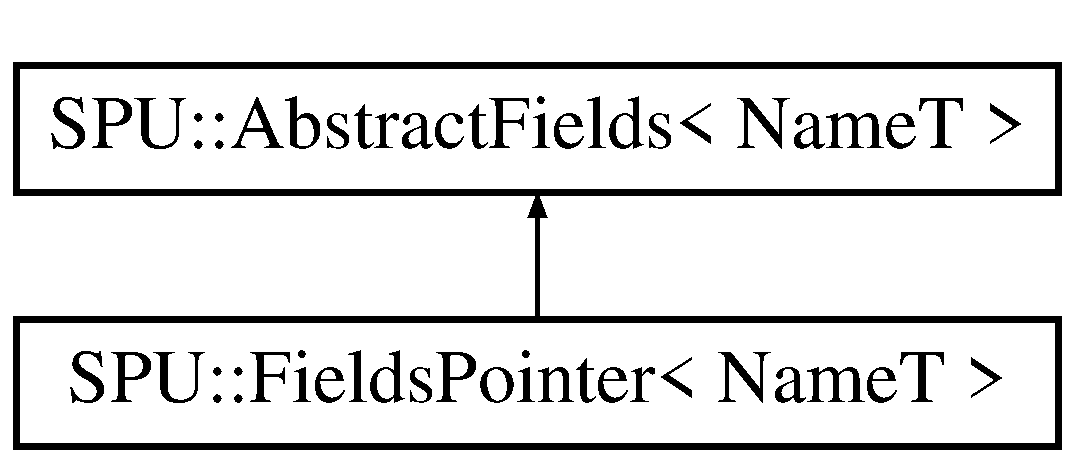
\includegraphics[height=2.000000cm]{class_s_p_u_1_1_abstract_fields}
\end{center}
\end{figure}
\doxysubsection*{Открытые члены}
\begin{DoxyCompactItemize}
\item 
\mbox{\Hypertarget{class_s_p_u_1_1_abstract_fields_ab6d58eb6fe239d4e56d3214c7e8ad10d}\label{class_s_p_u_1_1_abstract_fields_ab6d58eb6fe239d4e56d3214c7e8ad10d}} 
virtual {\bfseries operator data\+\_\+t} ()=0
\item 
\mbox{\Hypertarget{class_s_p_u_1_1_abstract_fields_a321cce6de1e8d8597f271f45a273c0a6}\label{class_s_p_u_1_1_abstract_fields_a321cce6de1e8d8597f271f45a273c0a6}} 
virtual \mbox{\hyperlink{class_s_p_u_1_1_abstract_fields}{Abstract\+Fields}} \& {\bfseries operator=} (data\+\_\+t fields\+\_\+data)=0
\item 
\mbox{\Hypertarget{class_s_p_u_1_1_abstract_fields_a5634bfa57050c2bb3ac57d5b5ce9e479}\label{class_s_p_u_1_1_abstract_fields_a5634bfa57050c2bb3ac57d5b5ce9e479}} 
virtual \mbox{\hyperlink{class_s_p_u_1_1_abstract_fields}{Abstract\+Fields}} \& {\bfseries operator=} (\mbox{\hyperlink{class_s_p_u_1_1_fields_data}{Data}} fields\+\_\+data)=0
\item 
\mbox{\Hypertarget{class_s_p_u_1_1_abstract_fields_aca06b1d47b10b3dbca1059c81e70e85c}\label{class_s_p_u_1_1_abstract_fields_aca06b1d47b10b3dbca1059c81e70e85c}} 
virtual data\+\_\+t \& {\bfseries operator\mbox{[}$\,$\mbox{]}} (NameT name)=0
\end{DoxyCompactItemize}
\doxysubsection*{Защищенные типы}
\begin{DoxyCompactItemize}
\item 
\mbox{\Hypertarget{class_s_p_u_1_1_abstract_fields_ac586104835d088869e6c66a00f52fb71}\label{class_s_p_u_1_1_abstract_fields_ac586104835d088869e6c66a00f52fb71}} 
using {\bfseries Length} = \mbox{\hyperlink{class_s_p_u_1_1_fields_length}{Fields\+Length}}$<$ NameT $>$
\item 
\mbox{\Hypertarget{class_s_p_u_1_1_abstract_fields_acf6cee1ea5388266f017e277dbaf78ef}\label{class_s_p_u_1_1_abstract_fields_acf6cee1ea5388266f017e277dbaf78ef}} 
using {\bfseries Data} = \mbox{\hyperlink{class_s_p_u_1_1_fields_data}{Fields\+Data}}$<$ NameT $>$
\end{DoxyCompactItemize}


Объявления и описания членов класса находятся в файле\+:\begin{DoxyCompactItemize}
\item 
spu-\/api/libspu/abstract\+\_\+fields.\+hpp\end{DoxyCompactItemize}

\hypertarget{class_s_p_u_1_1_abstract_fields_3_01void_01_4}{}\doxysection{Класс S\+PU\+::Abstract\+Fields$<$ void $>$}
\label{class_s_p_u_1_1_abstract_fields_3_01void_01_4}\index{SPU::AbstractFields$<$ void $>$@{SPU::AbstractFields$<$ void $>$}}
Граф наследования\+:S\+PU\+::Abstract\+Fields$<$ void $>$\+:\begin{figure}[H]
\begin{center}
\leavevmode
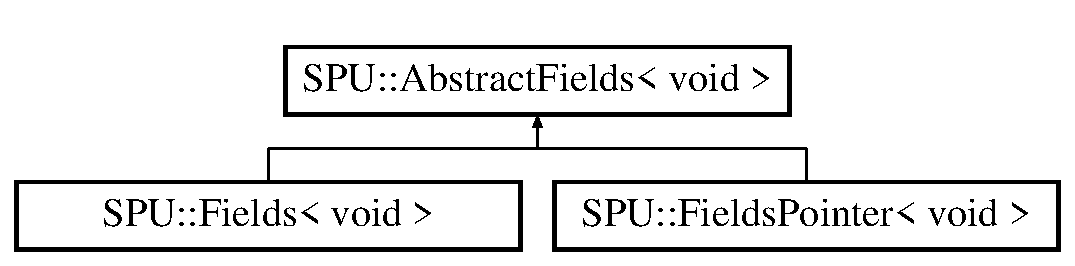
\includegraphics[height=2.000000cm]{class_s_p_u_1_1_abstract_fields_3_01void_01_4}
\end{center}
\end{figure}


Объявления и описания членов класса находятся в файле\+:\begin{DoxyCompactItemize}
\item 
spu-\/api/libspu/abstract\+\_\+fields.\+hpp\end{DoxyCompactItemize}

\hypertarget{class_s_p_u_1_1_abstract_structure}{}\section{Класс S\+PU\+:\+:Abstract\+Structure}
\label{class_s_p_u_1_1_abstract_structure}\index{S\+P\+U\+::\+Abstract\+Structure@{S\+P\+U\+::\+Abstract\+Structure}}
Граф наследования\+:S\+PU\+:\+:Abstract\+Structure\+:\begin{figure}[H]
\begin{center}
\leavevmode
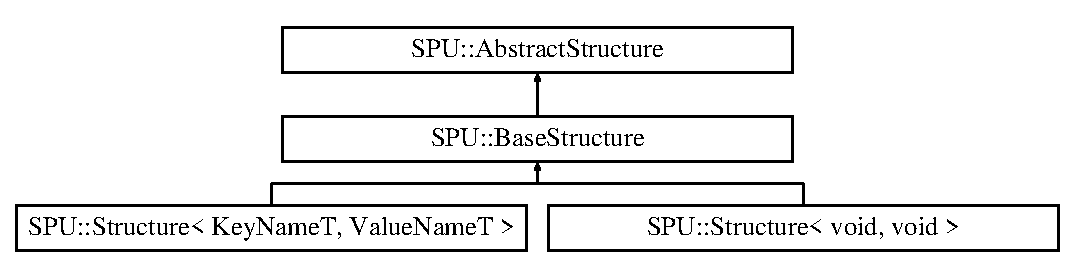
\includegraphics[height=3.000000cm]{class_s_p_u_1_1_abstract_structure}
\end{center}
\end{figure}
\subsection*{Классы}
\begin{DoxyCompactItemize}
\item 
struct \hyperlink{struct_s_p_u_1_1_abstract_structure_1_1_insert_struct}{Insert\+Struct}
\end{DoxyCompactItemize}
\subsection*{Открытые типы}
\begin{DoxyCompactItemize}
\item 
\mbox{\Hypertarget{class_s_p_u_1_1_abstract_structure_aa6f066b5548474e4330fb9439de690b5}\label{class_s_p_u_1_1_abstract_structure_aa6f066b5548474e4330fb9439de690b5}} 
using {\bfseries Insert\+Vector} = std\+::vector$<$ \hyperlink{struct_s_p_u_1_1_abstract_structure_1_1_insert_struct}{Insert\+Struct} $>$
\end{DoxyCompactItemize}
\subsection*{Открытые члены}
\begin{DoxyCompactItemize}
\item 
\mbox{\Hypertarget{class_s_p_u_1_1_abstract_structure_aad5e68309c8b463aa12642388f42d822}\label{class_s_p_u_1_1_abstract_structure_aad5e68309c8b463aa12642388f42d822}} 
virtual u32 {\bfseries get\+\_\+power} ()=0
\item 
\mbox{\Hypertarget{class_s_p_u_1_1_abstract_structure_a8c46ff9efeee7a4ff6cdf54e5190d818}\label{class_s_p_u_1_1_abstract_structure_a8c46ff9efeee7a4ff6cdf54e5190d818}} 
virtual status\+\_\+t {\bfseries insert} (key\+\_\+t key, value\+\_\+t value, flags\+\_\+t flags=N\+O\+\_\+\+F\+L\+A\+GS)=0
\item 
\mbox{\Hypertarget{class_s_p_u_1_1_abstract_structure_a948685f0124a3a0e49241dae8140e933}\label{class_s_p_u_1_1_abstract_structure_a948685f0124a3a0e49241dae8140e933}} 
virtual status\+\_\+t {\bfseries del} (key\+\_\+t key, flags\+\_\+t flags=N\+O\+\_\+\+F\+L\+A\+GS)=0
\item 
\mbox{\Hypertarget{class_s_p_u_1_1_abstract_structure_a3b0f4c97011b6c5b9bd54bf3a6622cf3}\label{class_s_p_u_1_1_abstract_structure_a3b0f4c97011b6c5b9bd54bf3a6622cf3}} 
virtual \hyperlink{struct_s_p_u_1_1pair__containter}{pair\+\_\+t} {\bfseries search} (key\+\_\+t key, flags\+\_\+t flags=P\+\_\+\+F\+L\+AG)=0
\item 
\mbox{\Hypertarget{class_s_p_u_1_1_abstract_structure_a6613408cebd3a985023433734f32fcf0}\label{class_s_p_u_1_1_abstract_structure_a6613408cebd3a985023433734f32fcf0}} 
virtual \hyperlink{struct_s_p_u_1_1pair__containter}{pair\+\_\+t} {\bfseries min} (flags\+\_\+t flags=P\+\_\+\+F\+L\+AG)=0
\item 
\mbox{\Hypertarget{class_s_p_u_1_1_abstract_structure_a7f0a85be53dd8b365fbad64aa5a5f3ee}\label{class_s_p_u_1_1_abstract_structure_a7f0a85be53dd8b365fbad64aa5a5f3ee}} 
virtual \hyperlink{struct_s_p_u_1_1pair__containter}{pair\+\_\+t} {\bfseries max} (flags\+\_\+t flags=P\+\_\+\+F\+L\+AG)=0
\item 
\mbox{\Hypertarget{class_s_p_u_1_1_abstract_structure_ac042dc48dd2b6bf63fc798ea291b4ce7}\label{class_s_p_u_1_1_abstract_structure_ac042dc48dd2b6bf63fc798ea291b4ce7}} 
virtual \hyperlink{struct_s_p_u_1_1pair__containter}{pair\+\_\+t} {\bfseries next} (key\+\_\+t key, flags\+\_\+t flags=P\+\_\+\+F\+L\+AG)=0
\item 
\mbox{\Hypertarget{class_s_p_u_1_1_abstract_structure_a5569186fd80dbfe74b13c274ffac8e41}\label{class_s_p_u_1_1_abstract_structure_a5569186fd80dbfe74b13c274ffac8e41}} 
virtual \hyperlink{struct_s_p_u_1_1pair__containter}{pair\+\_\+t} {\bfseries prev} (key\+\_\+t key, flags\+\_\+t flags=P\+\_\+\+F\+L\+AG)=0
\item 
\mbox{\Hypertarget{class_s_p_u_1_1_abstract_structure_af4d912aaacd609f571c1e3125ca8c6bf}\label{class_s_p_u_1_1_abstract_structure_af4d912aaacd609f571c1e3125ca8c6bf}} 
virtual \hyperlink{struct_s_p_u_1_1pair__containter}{pair\+\_\+t} {\bfseries nsm} (key\+\_\+t key, flags\+\_\+t flags=P\+\_\+\+F\+L\+AG)=0
\item 
\mbox{\Hypertarget{class_s_p_u_1_1_abstract_structure_af46e8bf350be4a504ba492bf3984568e}\label{class_s_p_u_1_1_abstract_structure_af46e8bf350be4a504ba492bf3984568e}} 
virtual \hyperlink{struct_s_p_u_1_1pair__containter}{pair\+\_\+t} {\bfseries ngr} (key\+\_\+t key, flags\+\_\+t flags=P\+\_\+\+F\+L\+AG)=0
\item 
\mbox{\Hypertarget{class_s_p_u_1_1_abstract_structure_af1f3aec8e4899b17744bbbbe7093050a}\label{class_s_p_u_1_1_abstract_structure_af1f3aec8e4899b17744bbbbe7093050a}} 
\hyperlink{structgsid__container}{gsid\+\_\+t} {\bfseries get\+\_\+gsid} ()
\item 
\mbox{\Hypertarget{class_s_p_u_1_1_abstract_structure_a98e992aa4e41aaa276d1b1ef54521e05}\label{class_s_p_u_1_1_abstract_structure_a98e992aa4e41aaa276d1b1ef54521e05}} 
status\+\_\+t {\bfseries insert\+Vector} (Insert\+Vector insert\+\_\+vector, flags\+\_\+t flags=N\+O\+\_\+\+F\+L\+A\+GS)
\end{DoxyCompactItemize}
\subsection*{Защищенные члены}
\begin{DoxyCompactItemize}
\item 
\mbox{\Hypertarget{class_s_p_u_1_1_abstract_structure_a9b717355192df2a255bf4925f0c1f75b}\label{class_s_p_u_1_1_abstract_structure_a9b717355192df2a255bf4925f0c1f75b}} 
virtual \hyperlink{structrsltfrmt__0}{adds\+\_\+rslt\+\_\+t} {\bfseries adds} ()=0
\item 
\mbox{\Hypertarget{class_s_p_u_1_1_abstract_structure_a818241d315d330a23dcfbed10630b4be}\label{class_s_p_u_1_1_abstract_structure_a818241d315d330a23dcfbed10630b4be}} 
virtual \hyperlink{structrsltfrmt__1}{dels\+\_\+rslt\+\_\+t} {\bfseries dels} ()=0
\end{DoxyCompactItemize}
\subsection*{Защищенные данные}
\begin{DoxyCompactItemize}
\item 
\mbox{\Hypertarget{class_s_p_u_1_1_abstract_structure_a6c31f84ff4323aad1ebc3690ccc0d3cc}\label{class_s_p_u_1_1_abstract_structure_a6c31f84ff4323aad1ebc3690ccc0d3cc}} 
\hyperlink{structgsid__container}{gsid\+\_\+t} {\bfseries gsid} = \{ 0 \}
\end{DoxyCompactItemize}


Объявления и описания членов класса находятся в файле\+:\begin{DoxyCompactItemize}
\item 
spu-\/api/libspu/abstract\+\_\+structure.\+hpp\end{DoxyCompactItemize}

\hypertarget{class_s_p_u___g_r_a_p_h_1_1_spu_ultra_graph_1_1_adjacent_edges}{}\doxysection{Шаблон класса S\+P\+U\+\_\+\+G\+R\+A\+PH\+::Spu\+Ultra\+Graph\+::Adjacent\+Edges$<$ I $>$}
\label{class_s_p_u___g_r_a_p_h_1_1_spu_ultra_graph_1_1_adjacent_edges}\index{SPU\_GRAPH::SpuUltraGraph::AdjacentEdges$<$ I $>$@{SPU\_GRAPH::SpuUltraGraph::AdjacentEdges$<$ I $>$}}


Контейнер содержащий смежные ребра для вершины v.  




{\ttfamily \#include $<$Spu\+Ultra\+Graph.\+h$>$}

\doxysubsection*{Открытые типы}
\begin{DoxyCompactItemize}
\item 
\mbox{\Hypertarget{class_s_p_u___g_r_a_p_h_1_1_spu_ultra_graph_1_1_adjacent_edges_a07295019466b1a51334abb9cfcfbef0c}\label{class_s_p_u___g_r_a_p_h_1_1_spu_ultra_graph_1_1_adjacent_edges_a07295019466b1a51334abb9cfcfbef0c}} 
typedef \mbox{\hyperlink{class_s_p_u___g_r_a_p_h_1_1_spu_ultra_graph_1_1_adjacent_edges_iterator}{Adjacent\+Edges\+Iterator}}$<$ I $>$ {\bfseries iterator}
\end{DoxyCompactItemize}
\doxysubsection*{Открытые члены}
\begin{DoxyCompactItemize}
\item 
\mbox{\Hypertarget{class_s_p_u___g_r_a_p_h_1_1_spu_ultra_graph_1_1_adjacent_edges_ab2f7687136e079ac52f3c151dccbf8a5}\label{class_s_p_u___g_r_a_p_h_1_1_spu_ultra_graph_1_1_adjacent_edges_ab2f7687136e079ac52f3c151dccbf8a5}} 
{\bfseries Adjacent\+Edges} (const \mbox{\hyperlink{class_s_p_u___g_r_a_p_h_1_1_spu_ultra_graph}{Spu\+Ultra\+Graph}} $\ast$g, Spu\+Ultra\+Graph\+::vertex\+\_\+descriptor v)
\item 
\mbox{\Hypertarget{class_s_p_u___g_r_a_p_h_1_1_spu_ultra_graph_1_1_adjacent_edges_a2a1ec5c277a774b0978909916bf31917}\label{class_s_p_u___g_r_a_p_h_1_1_spu_ultra_graph_1_1_adjacent_edges_a2a1ec5c277a774b0978909916bf31917}} 
\mbox{\hyperlink{class_s_p_u___g_r_a_p_h_1_1_spu_ultra_graph_1_1_adjacent_edges_iterator}{iterator}} {\bfseries begin} ()
\item 
\mbox{\Hypertarget{class_s_p_u___g_r_a_p_h_1_1_spu_ultra_graph_1_1_adjacent_edges_aa8fd47a34331b8acfc3a1c521117a871}\label{class_s_p_u___g_r_a_p_h_1_1_spu_ultra_graph_1_1_adjacent_edges_aa8fd47a34331b8acfc3a1c521117a871}} 
\mbox{\hyperlink{class_s_p_u___g_r_a_p_h_1_1_spu_ultra_graph_1_1_adjacent_edges_iterator}{iterator}} {\bfseries end} ()
\item 
\mbox{\Hypertarget{class_s_p_u___g_r_a_p_h_1_1_spu_ultra_graph_1_1_adjacent_edges_aec67d36c50e3a8d60009bf1235649592}\label{class_s_p_u___g_r_a_p_h_1_1_spu_ultra_graph_1_1_adjacent_edges_aec67d36c50e3a8d60009bf1235649592}} 
\mbox{\hyperlink{class_s_p_u___g_r_a_p_h_1_1_spu_ultra_graph_1_1_adjacent_edges_iterator}{iterator}} {\bfseries rbegin} ()
\item 
\mbox{\Hypertarget{class_s_p_u___g_r_a_p_h_1_1_spu_ultra_graph_1_1_adjacent_edges_a80cb7b7abd364fd292595a2e3e00f83e}\label{class_s_p_u___g_r_a_p_h_1_1_spu_ultra_graph_1_1_adjacent_edges_a80cb7b7abd364fd292595a2e3e00f83e}} 
\mbox{\hyperlink{class_s_p_u___g_r_a_p_h_1_1_spu_ultra_graph_1_1_adjacent_edges_iterator}{iterator}} {\bfseries rend} ()
\end{DoxyCompactItemize}


\doxysubsection{Подробное описание}
\subsubsection*{template$<$int I$>$\newline
class S\+P\+U\+\_\+\+G\+R\+A\+P\+H\+::\+Spu\+Ultra\+Graph\+::\+Adjacent\+Edges$<$ I $>$}

Контейнер содержащий смежные ребра для вершины v. 

Объявления и описания членов класса находятся в файле\+:\begin{DoxyCompactItemize}
\item 
Spu\+Ultra\+Graph.\+h\end{DoxyCompactItemize}

\hypertarget{class_s_p_u___g_r_a_p_h_1_1_spu_ultra_graph_1_1_adjacent_edges_iterator}{}\section{Шаблон класса S\+P\+U\+\_\+\+G\+R\+A\+PH\+:\+:Spu\+Ultra\+Graph\+:\+:Adjacent\+Edges\+Iterator$<$ I $>$}
\label{class_s_p_u___g_r_a_p_h_1_1_spu_ultra_graph_1_1_adjacent_edges_iterator}\index{S\+P\+U\+\_\+\+G\+R\+A\+P\+H\+::\+Spu\+Ultra\+Graph\+::\+Adjacent\+Edges\+Iterator$<$ I $>$@{S\+P\+U\+\_\+\+G\+R\+A\+P\+H\+::\+Spu\+Ultra\+Graph\+::\+Adjacent\+Edges\+Iterator$<$ I $>$}}
Граф наследования\+:S\+P\+U\+\_\+\+G\+R\+A\+PH\+:\+:Spu\+Ultra\+Graph\+:\+:Adjacent\+Edges\+Iterator$<$ I $>$\+:\begin{figure}[H]
\begin{center}
\leavevmode
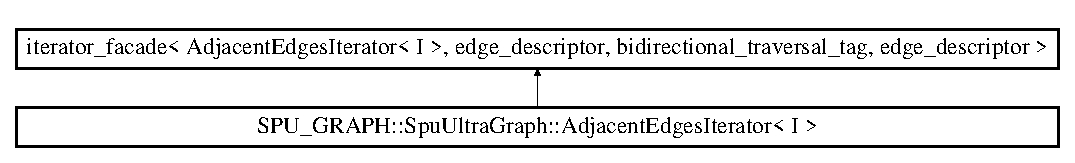
\includegraphics[height=1.741835cm]{class_s_p_u___g_r_a_p_h_1_1_spu_ultra_graph_1_1_adjacent_edges_iterator}
\end{center}
\end{figure}
\subsection*{Открытые члены}
\begin{DoxyCompactItemize}
\item 
\mbox{\Hypertarget{class_s_p_u___g_r_a_p_h_1_1_spu_ultra_graph_1_1_adjacent_edges_iterator_a64417e40bc04bd78e60c67411e7a5ce8}\label{class_s_p_u___g_r_a_p_h_1_1_spu_ultra_graph_1_1_adjacent_edges_iterator_a64417e40bc04bd78e60c67411e7a5ce8}} 
{\bfseries Adjacent\+Edges\+Iterator} (const \hyperlink{class_s_p_u___g_r_a_p_h_1_1_spu_ultra_graph}{Spu\+Ultra\+Graph} $\ast$g, vertex\+\_\+descriptor v, \hyperlink{class_s_p_u___g_r_a_p_h_1_1_spu_ultra_graph_a5f3776e003ef0a1648f1d9f84289810b}{edge\+\_\+descriptor} \hyperlink{class_s_p_u___g_r_a_p_h_1_1_spu_ultra_graph_a51468aa2278d3abb0c338ffbeac7747a}{edge}=0)
\item 
\mbox{\Hypertarget{class_s_p_u___g_r_a_p_h_1_1_spu_ultra_graph_1_1_adjacent_edges_iterator_a656e4ee28307ec462bc32500a0d81ff7}\label{class_s_p_u___g_r_a_p_h_1_1_spu_ultra_graph_1_1_adjacent_edges_iterator_a656e4ee28307ec462bc32500a0d81ff7}} 
\hyperlink{class_s_p_u___g_r_a_p_h_1_1_spu_ultra_graph_a5f3776e003ef0a1648f1d9f84289810b}{edge\+\_\+descriptor} {\bfseries dereference} () const
\item 
\mbox{\Hypertarget{class_s_p_u___g_r_a_p_h_1_1_spu_ultra_graph_1_1_adjacent_edges_iterator_a28ed894caf491d7a9b66e97b9724ee2b}\label{class_s_p_u___g_r_a_p_h_1_1_spu_ultra_graph_1_1_adjacent_edges_iterator_a28ed894caf491d7a9b66e97b9724ee2b}} 
bool {\bfseries equal} (const \hyperlink{class_s_p_u___g_r_a_p_h_1_1_spu_ultra_graph_1_1_adjacent_edges_iterator}{Adjacent\+Edges\+Iterator} \&other) const
\item 
\mbox{\Hypertarget{class_s_p_u___g_r_a_p_h_1_1_spu_ultra_graph_1_1_adjacent_edges_iterator_ace201686851d7e5c4353afeddcd9c24d}\label{class_s_p_u___g_r_a_p_h_1_1_spu_ultra_graph_1_1_adjacent_edges_iterator_ace201686851d7e5c4353afeddcd9c24d}} 
void {\bfseries increment} ()
\item 
\mbox{\Hypertarget{class_s_p_u___g_r_a_p_h_1_1_spu_ultra_graph_1_1_adjacent_edges_iterator_ac96c7bfab4c3d631ca7499961bbc87a1}\label{class_s_p_u___g_r_a_p_h_1_1_spu_ultra_graph_1_1_adjacent_edges_iterator_ac96c7bfab4c3d631ca7499961bbc87a1}} 
void {\bfseries decrement} ()
\end{DoxyCompactItemize}
\subsection*{Друзья}
\begin{DoxyCompactItemize}
\item 
\mbox{\Hypertarget{class_s_p_u___g_r_a_p_h_1_1_spu_ultra_graph_1_1_adjacent_edges_iterator_a0975271623c74c5b89bdf8d7fbce69c4}\label{class_s_p_u___g_r_a_p_h_1_1_spu_ultra_graph_1_1_adjacent_edges_iterator_a0975271623c74c5b89bdf8d7fbce69c4}} 
class {\bfseries iterator\+\_\+core\+\_\+access}
\end{DoxyCompactItemize}


Объявления и описания членов класса находятся в файле\+:\begin{DoxyCompactItemize}
\item 
Spu\+Ultra\+Graph.\+h\end{DoxyCompactItemize}

\hypertarget{class_s_p_u___g_r_a_p_h_1_1_spu_ultra_graph_1_1_adjacent_vertices}{}\doxysection{Класс S\+P\+U\+\_\+\+G\+R\+A\+PH\+::Spu\+Ultra\+Graph\+::Adjacent\+Vertices}
\label{class_s_p_u___g_r_a_p_h_1_1_spu_ultra_graph_1_1_adjacent_vertices}\index{SPU\_GRAPH::SpuUltraGraph::AdjacentVertices@{SPU\_GRAPH::SpuUltraGraph::AdjacentVertices}}


Контейнер содержащий вершины смежные вершине v.  




{\ttfamily \#include $<$Spu\+Ultra\+Graph.\+h$>$}

\doxysubsection*{Открытые типы}
\begin{DoxyCompactItemize}
\item 
\mbox{\Hypertarget{class_s_p_u___g_r_a_p_h_1_1_spu_ultra_graph_1_1_adjacent_vertices_a12561c9d0f9fcf509dab4a5b61ffe1ff}\label{class_s_p_u___g_r_a_p_h_1_1_spu_ultra_graph_1_1_adjacent_vertices_a12561c9d0f9fcf509dab4a5b61ffe1ff}} 
typedef \mbox{\hyperlink{class_s_p_u___g_r_a_p_h_1_1_spu_ultra_graph_ae50dab54e277cf22d3e318d468e7585c}{adjacency\+\_\+iterator}} {\bfseries iterator}
\end{DoxyCompactItemize}
\doxysubsection*{Открытые члены}
\begin{DoxyCompactItemize}
\item 
\mbox{\Hypertarget{class_s_p_u___g_r_a_p_h_1_1_spu_ultra_graph_1_1_adjacent_vertices_a63ae31425be10389d7e5b7a7f8dbf275}\label{class_s_p_u___g_r_a_p_h_1_1_spu_ultra_graph_1_1_adjacent_vertices_a63ae31425be10389d7e5b7a7f8dbf275}} 
{\bfseries Adjacent\+Vertices} (const \mbox{\hyperlink{class_s_p_u___g_r_a_p_h_1_1_spu_ultra_graph}{Spu\+Ultra\+Graph}} $\ast$g, vertex\+\_\+descriptor v)
\item 
\mbox{\Hypertarget{class_s_p_u___g_r_a_p_h_1_1_spu_ultra_graph_1_1_adjacent_vertices_a08c87852160ae17145c945a8e74514f3}\label{class_s_p_u___g_r_a_p_h_1_1_spu_ultra_graph_1_1_adjacent_vertices_a08c87852160ae17145c945a8e74514f3}} 
\mbox{\hyperlink{class_s_p_u___g_r_a_p_h_1_1_spu_ultra_graph_1_1_adjacent_vertices_iterator}{iterator}} {\bfseries begin} ()
\item 
\mbox{\Hypertarget{class_s_p_u___g_r_a_p_h_1_1_spu_ultra_graph_1_1_adjacent_vertices_a6b40458eab68f1f541a0fc0462edd2ce}\label{class_s_p_u___g_r_a_p_h_1_1_spu_ultra_graph_1_1_adjacent_vertices_a6b40458eab68f1f541a0fc0462edd2ce}} 
\mbox{\hyperlink{class_s_p_u___g_r_a_p_h_1_1_spu_ultra_graph_1_1_adjacent_vertices_iterator}{iterator}} {\bfseries end} ()
\item 
\mbox{\Hypertarget{class_s_p_u___g_r_a_p_h_1_1_spu_ultra_graph_1_1_adjacent_vertices_a39a2953d72cb264f39f75673522680b7}\label{class_s_p_u___g_r_a_p_h_1_1_spu_ultra_graph_1_1_adjacent_vertices_a39a2953d72cb264f39f75673522680b7}} 
\mbox{\hyperlink{class_s_p_u___g_r_a_p_h_1_1_spu_ultra_graph_1_1_adjacent_vertices_iterator}{iterator}} {\bfseries rbegin} ()
\item 
\mbox{\Hypertarget{class_s_p_u___g_r_a_p_h_1_1_spu_ultra_graph_1_1_adjacent_vertices_a2a6b807d6fc5c812ffee8a98566d50a5}\label{class_s_p_u___g_r_a_p_h_1_1_spu_ultra_graph_1_1_adjacent_vertices_a2a6b807d6fc5c812ffee8a98566d50a5}} 
\mbox{\hyperlink{class_s_p_u___g_r_a_p_h_1_1_spu_ultra_graph_1_1_adjacent_vertices_iterator}{iterator}} {\bfseries rend} ()
\end{DoxyCompactItemize}


\doxysubsection{Подробное описание}
Контейнер содержащий вершины смежные вершине v. 

Объявления и описания членов класса находятся в файле\+:\begin{DoxyCompactItemize}
\item 
Spu\+Ultra\+Graph.\+h\end{DoxyCompactItemize}

\hypertarget{class_s_p_u___g_r_a_p_h_1_1_spu_ultra_graph_1_1_adjacent_vertices_iterator}{}\doxysection{Класс S\+P\+U\+\_\+\+G\+R\+A\+PH\+::Spu\+Ultra\+Graph\+::Adjacent\+Vertices\+Iterator}
\label{class_s_p_u___g_r_a_p_h_1_1_spu_ultra_graph_1_1_adjacent_vertices_iterator}\index{SPU\_GRAPH::SpuUltraGraph::AdjacentVerticesIterator@{SPU\_GRAPH::SpuUltraGraph::AdjacentVerticesIterator}}


{\ttfamily \#include $<$Spu\+Ultra\+Graph.\+h$>$}

Граф наследования\+:S\+P\+U\+\_\+\+G\+R\+A\+PH\+::Spu\+Ultra\+Graph\+::Adjacent\+Vertices\+Iterator\+:\begin{figure}[H]
\begin{center}
\leavevmode
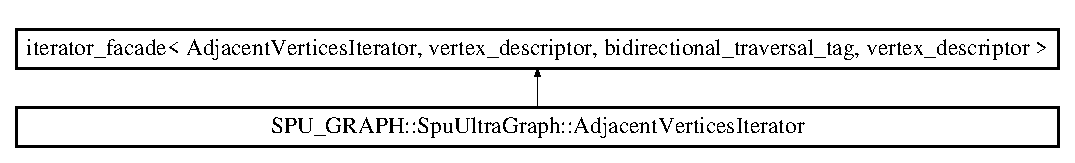
\includegraphics[height=1.744548cm]{class_s_p_u___g_r_a_p_h_1_1_spu_ultra_graph_1_1_adjacent_vertices_iterator}
\end{center}
\end{figure}
\doxysubsection*{Открытые члены}
\begin{DoxyCompactItemize}
\item 
\mbox{\hyperlink{class_s_p_u___g_r_a_p_h_1_1_spu_ultra_graph_1_1_adjacent_vertices_iterator_a925cadcc4cf9412ffad955f052bbfe85}{Adjacent\+Vertices\+Iterator}} (const \mbox{\hyperlink{class_s_p_u___g_r_a_p_h_1_1_spu_ultra_graph}{Spu\+Ultra\+Graph}} $\ast$g=nullptr, vertex\+\_\+descriptor v=0, \mbox{\hyperlink{class_s_p_u___g_r_a_p_h_1_1_spu_ultra_graph_a5f3776e003ef0a1648f1d9f84289810b}{edge\+\_\+descriptor}} e=0, vertex\+\_\+descriptor u=0)
\item 
\mbox{\Hypertarget{class_s_p_u___g_r_a_p_h_1_1_spu_ultra_graph_1_1_adjacent_vertices_iterator_a392deba0b5335898f49347e119b34b44}\label{class_s_p_u___g_r_a_p_h_1_1_spu_ultra_graph_1_1_adjacent_vertices_iterator_a392deba0b5335898f49347e119b34b44}} 
vertex\+\_\+descriptor {\bfseries dereference} () const
\item 
\mbox{\Hypertarget{class_s_p_u___g_r_a_p_h_1_1_spu_ultra_graph_1_1_adjacent_vertices_iterator_ad8ce4cef0876df909845be2b4f284f9e}\label{class_s_p_u___g_r_a_p_h_1_1_spu_ultra_graph_1_1_adjacent_vertices_iterator_ad8ce4cef0876df909845be2b4f284f9e}} 
bool {\bfseries equal} (const \mbox{\hyperlink{class_s_p_u___g_r_a_p_h_1_1_spu_ultra_graph_1_1_adjacent_vertices_iterator}{Adjacent\+Vertices\+Iterator}} \&other) const
\item 
\mbox{\Hypertarget{class_s_p_u___g_r_a_p_h_1_1_spu_ultra_graph_1_1_adjacent_vertices_iterator_a568b6ac3fa6cda300c434d8772508387}\label{class_s_p_u___g_r_a_p_h_1_1_spu_ultra_graph_1_1_adjacent_vertices_iterator_a568b6ac3fa6cda300c434d8772508387}} 
void {\bfseries increment} ()
\item 
\mbox{\Hypertarget{class_s_p_u___g_r_a_p_h_1_1_spu_ultra_graph_1_1_adjacent_vertices_iterator_ab4879ad89bd0493e7d836f5dc715619b}\label{class_s_p_u___g_r_a_p_h_1_1_spu_ultra_graph_1_1_adjacent_vertices_iterator_ab4879ad89bd0493e7d836f5dc715619b}} 
void {\bfseries decrement} ()
\end{DoxyCompactItemize}
\doxysubsection*{Друзья}
\begin{DoxyCompactItemize}
\item 
\mbox{\Hypertarget{class_s_p_u___g_r_a_p_h_1_1_spu_ultra_graph_1_1_adjacent_vertices_iterator_a0975271623c74c5b89bdf8d7fbce69c4}\label{class_s_p_u___g_r_a_p_h_1_1_spu_ultra_graph_1_1_adjacent_vertices_iterator_a0975271623c74c5b89bdf8d7fbce69c4}} 
class {\bfseries iterator\+\_\+core\+\_\+access}
\end{DoxyCompactItemize}


\doxysubsection{Подробное описание}
Итератор по вершинам смежным вершине v Итератор проходит по всем ребрам исходящих от v, т.\+о. при прохождении по параллельным ребрам будут повторяться вершины 

\doxysubsection{Конструктор(ы)}
\mbox{\Hypertarget{class_s_p_u___g_r_a_p_h_1_1_spu_ultra_graph_1_1_adjacent_vertices_iterator_a925cadcc4cf9412ffad955f052bbfe85}\label{class_s_p_u___g_r_a_p_h_1_1_spu_ultra_graph_1_1_adjacent_vertices_iterator_a925cadcc4cf9412ffad955f052bbfe85}} 
\index{SPU\_GRAPH::SpuUltraGraph::AdjacentVerticesIterator@{SPU\_GRAPH::SpuUltraGraph::AdjacentVerticesIterator}!AdjacentVerticesIterator@{AdjacentVerticesIterator}}
\index{AdjacentVerticesIterator@{AdjacentVerticesIterator}!SPU\_GRAPH::SpuUltraGraph::AdjacentVerticesIterator@{SPU\_GRAPH::SpuUltraGraph::AdjacentVerticesIterator}}
\doxysubsubsection{\texorpdfstring{AdjacentVerticesIterator()}{AdjacentVerticesIterator()}}
{\footnotesize\ttfamily S\+P\+U\+\_\+\+G\+R\+A\+P\+H\+::\+Spu\+Ultra\+Graph\+::\+Adjacent\+Vertices\+Iterator\+::\+Adjacent\+Vertices\+Iterator (\begin{DoxyParamCaption}\item[{const \mbox{\hyperlink{class_s_p_u___g_r_a_p_h_1_1_spu_ultra_graph}{Spu\+Ultra\+Graph}} $\ast$}]{g = {\ttfamily nullptr},  }\item[{vertex\+\_\+descriptor}]{v = {\ttfamily 0},  }\item[{\mbox{\hyperlink{class_s_p_u___g_r_a_p_h_1_1_spu_ultra_graph_a5f3776e003ef0a1648f1d9f84289810b}{edge\+\_\+descriptor}}}]{e = {\ttfamily 0},  }\item[{vertex\+\_\+descriptor}]{u = {\ttfamily 0} }\end{DoxyParamCaption})\hspace{0.3cm}{\ttfamily [inline]}}

Конструктор итератора по вершинам смежным вершине v 
\begin{DoxyParams}{Аргументы}
{\em g} & Граф \\
\hline
{\em v} & Вершина относительно которой будет проходить итератор по смежным вершинам \\
\hline
{\em e} & Текущее ребро \\
\hline
{\em u} & Текущая вершина \\
\hline
\end{DoxyParams}


Объявления и описания членов классов находятся в файлах\+:\begin{DoxyCompactItemize}
\item 
Spu\+Ultra\+Graph.\+h\item 
Spu\+Ultra\+Graph.\+cpp\end{DoxyCompactItemize}

\hypertarget{class_bad_request}{}\section{Класс Bad\+Request}
\label{class_bad_request}\index{Bad\+Request@{Bad\+Request}}
Граф наследования\+:Bad\+Request\+:\begin{figure}[H]
\begin{center}
\leavevmode
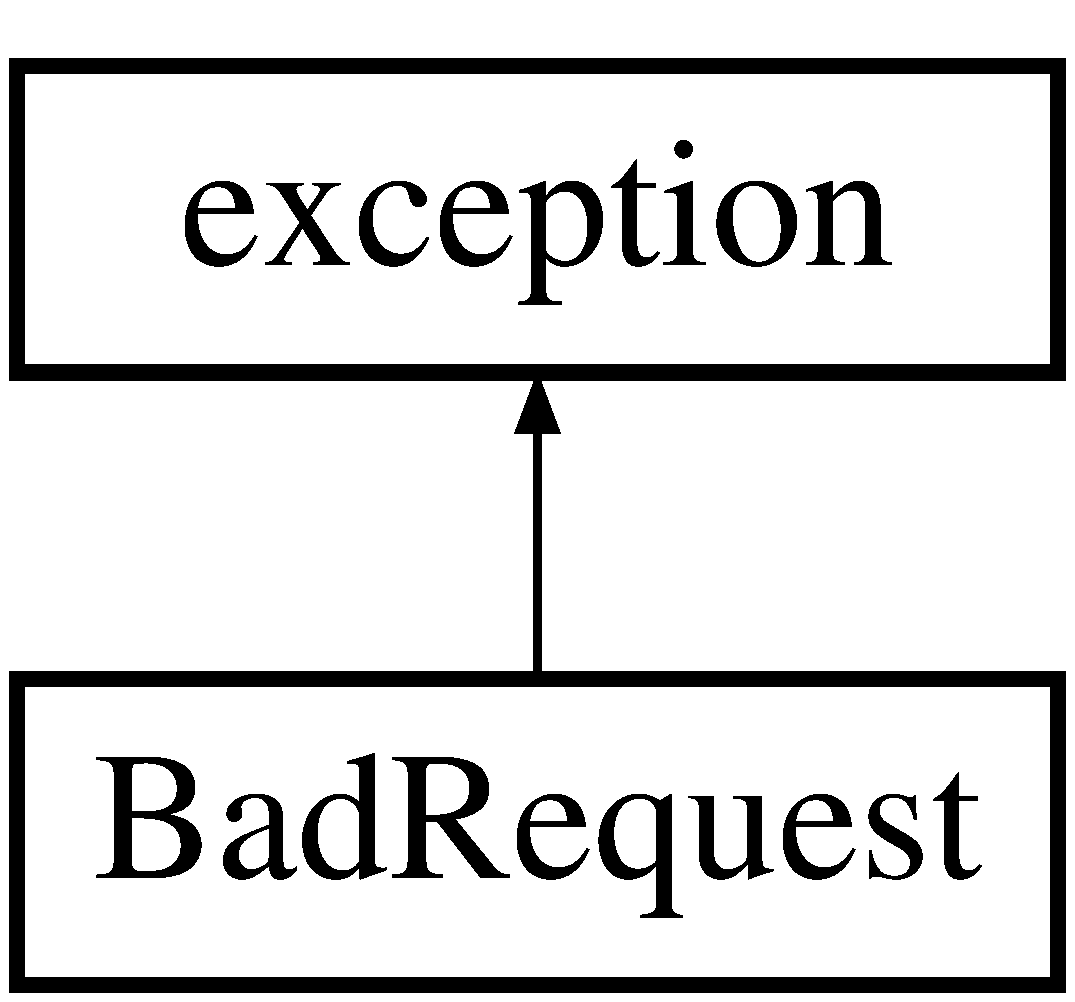
\includegraphics[height=2.000000cm]{class_bad_request}
\end{center}
\end{figure}
\subsection*{Открытые члены}
\begin{DoxyCompactItemize}
\item 
\mbox{\Hypertarget{class_bad_request_a9de00a98b3542f82f39179c11f50b68a}\label{class_bad_request_a9de00a98b3542f82f39179c11f50b68a}} 
{\bfseries Bad\+Request} (const string \&error=\char`\"{}Bad Request\char`\"{})
\item 
\mbox{\Hypertarget{class_bad_request_ae90e8414e00f29e64407a3451cfc0e34}\label{class_bad_request_ae90e8414e00f29e64407a3451cfc0e34}} 
const char $\ast$ {\bfseries what} () const noexcept override
\end{DoxyCompactItemize}


Объявления и описания членов класса находятся в файле\+:\begin{DoxyCompactItemize}
\item 
exceptions.\+h\end{DoxyCompactItemize}

\hypertarget{class_s_p_u_1_1_base_extern_value}{}\doxysection{Класс S\+PU\+::Base\+Extern\+Value}
\label{class_s_p_u_1_1_base_extern_value}\index{SPU::BaseExternValue@{SPU::BaseExternValue}}
Граф наследования\+:S\+PU\+::Base\+Extern\+Value\+:\begin{figure}[H]
\begin{center}
\leavevmode
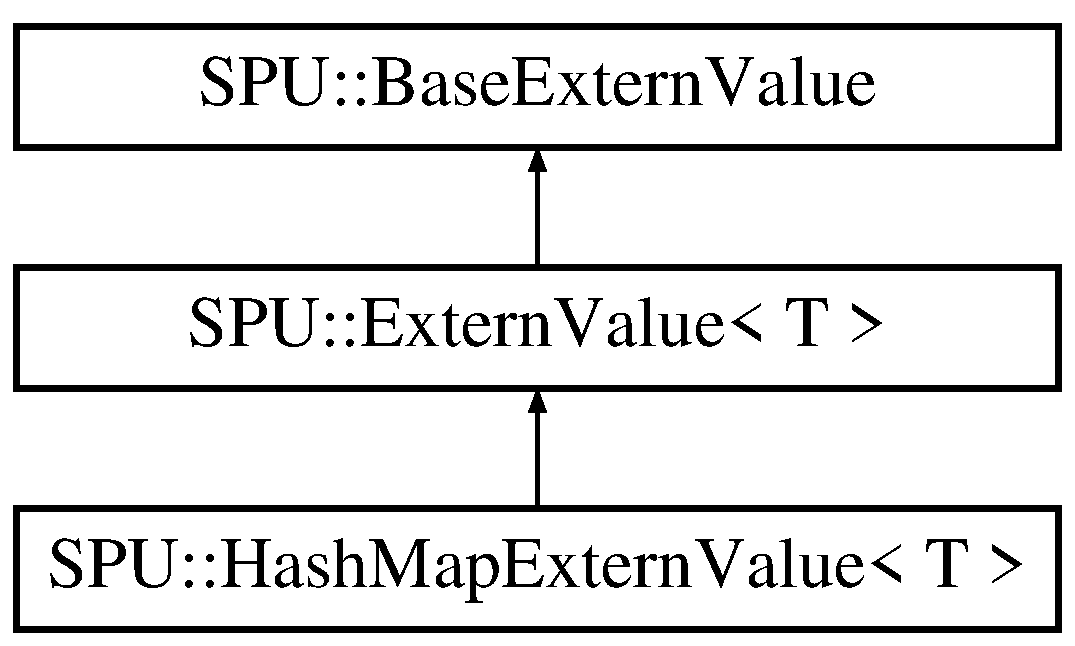
\includegraphics[height=3.000000cm]{class_s_p_u_1_1_base_extern_value}
\end{center}
\end{figure}
\doxysubsection*{Открытые члены}
\begin{DoxyCompactItemize}
\item 
\mbox{\Hypertarget{class_s_p_u_1_1_base_extern_value_ae9e51d018d0d35d805c8fdbd192ac5c7}\label{class_s_p_u_1_1_base_extern_value_ae9e51d018d0d35d805c8fdbd192ac5c7}} 
{\bfseries Base\+Extern\+Value} (value\+\_\+t id)
\item 
\mbox{\Hypertarget{class_s_p_u_1_1_base_extern_value_a9a43c99d29c04561ea539d12bae72d16}\label{class_s_p_u_1_1_base_extern_value_a9a43c99d29c04561ea539d12bae72d16}} 
value\+\_\+t {\bfseries get\+\_\+id} ()
\item 
\mbox{\Hypertarget{class_s_p_u_1_1_base_extern_value_a568e32ba8cc9977e5ad6545838b599dc}\label{class_s_p_u_1_1_base_extern_value_a568e32ba8cc9977e5ad6545838b599dc}} 
void {\bfseries set\+\_\+id} (value\+\_\+t id)
\item 
\mbox{\Hypertarget{class_s_p_u_1_1_base_extern_value_aa281e19470299ce9d622392d7d4fb9f2}\label{class_s_p_u_1_1_base_extern_value_aa281e19470299ce9d622392d7d4fb9f2}} 
{\bfseries operator data\+\_\+t} ()
\end{DoxyCompactItemize}
\doxysubsection*{Открытые статические члены}
\begin{DoxyCompactItemize}
\item 
\mbox{\Hypertarget{class_s_p_u_1_1_base_extern_value_aba9cadc3d83388611b757a6b14eb27e6}\label{class_s_p_u_1_1_base_extern_value_aba9cadc3d83388611b757a6b14eb27e6}} 
static void {\bfseries spu\+\_\+insert} (\mbox{\hyperlink{structgsid__container}{gsid\+\_\+t}} gsid, key\+\_\+t key, \mbox{\hyperlink{class_s_p_u_1_1_base_extern_value}{Base\+Extern\+Value}} \&value)
\item 
\mbox{\Hypertarget{class_s_p_u_1_1_base_extern_value_a96a28d828127bb86c7f91f135565b3ec}\label{class_s_p_u_1_1_base_extern_value_a96a28d828127bb86c7f91f135565b3ec}} 
static void {\bfseries spu\+\_\+remove} (\mbox{\hyperlink{structgsid__container}{gsid\+\_\+t}} gsid, key\+\_\+t key)
\end{DoxyCompactItemize}
\doxysubsection*{Защищенные члены}
\begin{DoxyCompactItemize}
\item 
\mbox{\Hypertarget{class_s_p_u_1_1_base_extern_value_a07a83e438eb4f53548f3382aace21b65}\label{class_s_p_u_1_1_base_extern_value_a07a83e438eb4f53548f3382aace21b65}} 
value\+\_\+t {\bfseries get\+\_\+next\+\_\+id} ()
\end{DoxyCompactItemize}


Объявления и описания членов классов находятся в файлах\+:\begin{DoxyCompactItemize}
\item 
spu-\/api/libspu/extern\+\_\+value.\+hpp\item 
spu-\/api/libspu/extern\+\_\+value.\+cpp\end{DoxyCompactItemize}

\hypertarget{class_s_p_u_1_1_base_structure}{}\section{Класс S\+PU\+:\+:Base\+Structure}
\label{class_s_p_u_1_1_base_structure}\index{S\+P\+U\+::\+Base\+Structure@{S\+P\+U\+::\+Base\+Structure}}
Граф наследования\+:S\+PU\+:\+:Base\+Structure\+:\begin{figure}[H]
\begin{center}
\leavevmode
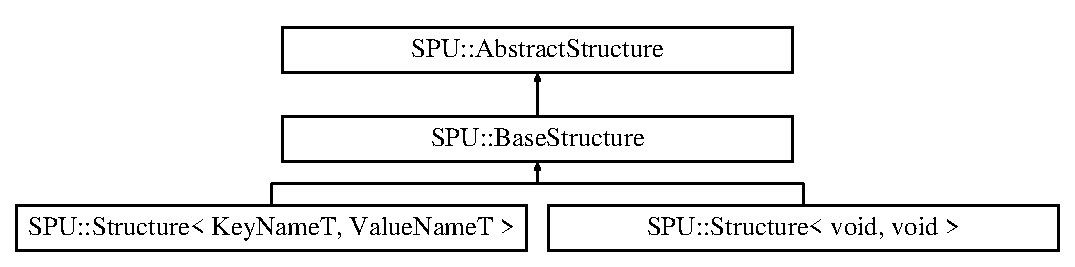
\includegraphics[height=3.000000cm]{class_s_p_u_1_1_base_structure}
\end{center}
\end{figure}
\subsection*{Открытые члены}
\begin{DoxyCompactItemize}
\item 
\mbox{\Hypertarget{class_s_p_u_1_1_base_structure_a38bc4a650b064ee7cf2b54b03f8dfebb}\label{class_s_p_u_1_1_base_structure_a38bc4a650b064ee7cf2b54b03f8dfebb}} 
u32 {\bfseries get\+\_\+power} () override
\item 
\mbox{\Hypertarget{class_s_p_u_1_1_base_structure_a34c1db5f750ad9a683426fe57516187a}\label{class_s_p_u_1_1_base_structure_a34c1db5f750ad9a683426fe57516187a}} 
status\+\_\+t {\bfseries insert} (key\+\_\+t key, value\+\_\+t value, flags\+\_\+t flags=N\+O\+\_\+\+F\+L\+A\+GS) override
\item 
\mbox{\Hypertarget{class_s_p_u_1_1_base_structure_a94c3b4f7e1dd49ebe715385373a06708}\label{class_s_p_u_1_1_base_structure_a94c3b4f7e1dd49ebe715385373a06708}} 
status\+\_\+t {\bfseries del} (key\+\_\+t key, flags\+\_\+t flags=N\+O\+\_\+\+F\+L\+A\+GS) override
\item 
\mbox{\Hypertarget{class_s_p_u_1_1_base_structure_a127f43b3ea999118e08ca797b42ac9ac}\label{class_s_p_u_1_1_base_structure_a127f43b3ea999118e08ca797b42ac9ac}} 
\hyperlink{struct_s_p_u_1_1pair__containter}{pair\+\_\+t} {\bfseries search} (key\+\_\+t key, flags\+\_\+t flags=P\+\_\+\+F\+L\+AG) override
\item 
\mbox{\Hypertarget{class_s_p_u_1_1_base_structure_a6c8e68accd0546286b2d783a1253e6c3}\label{class_s_p_u_1_1_base_structure_a6c8e68accd0546286b2d783a1253e6c3}} 
\hyperlink{struct_s_p_u_1_1pair__containter}{pair\+\_\+t} {\bfseries min} (flags\+\_\+t flags=P\+\_\+\+F\+L\+AG) override
\item 
\mbox{\Hypertarget{class_s_p_u_1_1_base_structure_a8dd831f527837a81aead1c14e60f8b85}\label{class_s_p_u_1_1_base_structure_a8dd831f527837a81aead1c14e60f8b85}} 
\hyperlink{struct_s_p_u_1_1pair__containter}{pair\+\_\+t} {\bfseries max} (flags\+\_\+t flags=P\+\_\+\+F\+L\+AG) override
\item 
\mbox{\Hypertarget{class_s_p_u_1_1_base_structure_a6a29d3ff930d608adebcd787fa60f16c}\label{class_s_p_u_1_1_base_structure_a6a29d3ff930d608adebcd787fa60f16c}} 
\hyperlink{struct_s_p_u_1_1pair__containter}{pair\+\_\+t} {\bfseries next} (key\+\_\+t key, flags\+\_\+t flags=P\+\_\+\+F\+L\+AG) override
\item 
\mbox{\Hypertarget{class_s_p_u_1_1_base_structure_af79a7465fb42e951e255c8fd2bddbbda}\label{class_s_p_u_1_1_base_structure_af79a7465fb42e951e255c8fd2bddbbda}} 
\hyperlink{struct_s_p_u_1_1pair__containter}{pair\+\_\+t} {\bfseries prev} (key\+\_\+t key, flags\+\_\+t flags=P\+\_\+\+F\+L\+AG) override
\item 
\mbox{\Hypertarget{class_s_p_u_1_1_base_structure_aca450d9d4de8a88d6dcbc567513f1f8e}\label{class_s_p_u_1_1_base_structure_aca450d9d4de8a88d6dcbc567513f1f8e}} 
\hyperlink{struct_s_p_u_1_1pair__containter}{pair\+\_\+t} {\bfseries nsm} (key\+\_\+t key, flags\+\_\+t flags=P\+\_\+\+F\+L\+AG) override
\item 
\mbox{\Hypertarget{class_s_p_u_1_1_base_structure_a58d7da2df970b961da73a36de2e3c026}\label{class_s_p_u_1_1_base_structure_a58d7da2df970b961da73a36de2e3c026}} 
\hyperlink{struct_s_p_u_1_1pair__containter}{pair\+\_\+t} {\bfseries ngr} (key\+\_\+t key, flags\+\_\+t flags=P\+\_\+\+F\+L\+AG) override
\end{DoxyCompactItemize}
\subsection*{Защищенные члены}
\begin{DoxyCompactItemize}
\item 
\mbox{\Hypertarget{class_s_p_u_1_1_base_structure_a35f88e6d609bfb752b7f6a630938b322}\label{class_s_p_u_1_1_base_structure_a35f88e6d609bfb752b7f6a630938b322}} 
\hyperlink{structrsltfrmt__0}{adds\+\_\+rslt\+\_\+t} {\bfseries adds} () override
\item 
\mbox{\Hypertarget{class_s_p_u_1_1_base_structure_a9c53aadd1b606fffc3aa72710e4b4d71}\label{class_s_p_u_1_1_base_structure_a9c53aadd1b606fffc3aa72710e4b4d71}} 
\hyperlink{structrsltfrmt__1}{dels\+\_\+rslt\+\_\+t} {\bfseries dels} () override
\end{DoxyCompactItemize}
\subsection*{Дополнительные унаследованные члены}


Объявления и описания членов классов находятся в файлах\+:\begin{DoxyCompactItemize}
\item 
spu-\/api/libspu/base\+\_\+structure.\+hpp\item 
spu-\/api/libspu/base\+\_\+structure.\+cpp\end{DoxyCompactItemize}

\hypertarget{structcmdfrmt__0}{}\doxysection{Структура cmdfrmt\+\_\+0}
\label{structcmdfrmt__0}\index{cmdfrmt\_0@{cmdfrmt\_0}}
\doxysubsection*{Открытые атрибуты}
\begin{DoxyCompactItemize}
\item 
\mbox{\Hypertarget{structcmdfrmt__0_a86c8257196b38bf4a7b6118d29ca8c8a}\label{structcmdfrmt__0_a86c8257196b38bf4a7b6118d29ca8c8a}} 
u8 {\bfseries cmd}
\end{DoxyCompactItemize}


Объявления и описания членов структуры находятся в файле\+:\begin{DoxyCompactItemize}
\item 
spu-\/api/libspu/spu.\+h\end{DoxyCompactItemize}

\hypertarget{structcmdfrmt__1}{}\doxysection{Структура cmdfrmt\+\_\+1}
\label{structcmdfrmt__1}\index{cmdfrmt\_1@{cmdfrmt\_1}}
\doxysubsection*{Открытые атрибуты}
\begin{DoxyCompactItemize}
\item 
\mbox{\Hypertarget{structcmdfrmt__1_acc1996761c336111cb475a6207678ca4}\label{structcmdfrmt__1_acc1996761c336111cb475a6207678ca4}} 
cmd\+\_\+t {\bfseries cmd}
\item 
\mbox{\Hypertarget{structcmdfrmt__1_af12fc67fc18a5b127e65590130e063b6}\label{structcmdfrmt__1_af12fc67fc18a5b127e65590130e063b6}} 
\mbox{\hyperlink{structgsid__container}{gsid\+\_\+t}} {\bfseries gsid}
\item 
\mbox{\Hypertarget{structcmdfrmt__1_a242c09c1c182e065ee9a2bb2de04aa84}\label{structcmdfrmt__1_a242c09c1c182e065ee9a2bb2de04aa84}} 
\mbox{\hyperlink{structdata__container}{spu\+\_\+key\+\_\+t}} {\bfseries key}
\item 
\mbox{\Hypertarget{structcmdfrmt__1_a0f1b3511c9911ff6fdfcb2e604f55dba}\label{structcmdfrmt__1_a0f1b3511c9911ff6fdfcb2e604f55dba}} 
\mbox{\hyperlink{structdata__container}{val\+\_\+t}} {\bfseries val}
\end{DoxyCompactItemize}


Объявления и описания членов структуры находятся в файле\+:\begin{DoxyCompactItemize}
\item 
spu-\/api/libspu/spu.\+h\end{DoxyCompactItemize}

\hypertarget{structcmdfrmt__2}{}\doxysection{Структура cmdfrmt\+\_\+2}
\label{structcmdfrmt__2}\index{cmdfrmt\_2@{cmdfrmt\_2}}
\doxysubsection*{Открытые атрибуты}
\begin{DoxyCompactItemize}
\item 
\mbox{\Hypertarget{structcmdfrmt__2_adab70b9e159adb970b2f883bb3d6b1f7}\label{structcmdfrmt__2_adab70b9e159adb970b2f883bb3d6b1f7}} 
cmd\+\_\+t {\bfseries cmd}
\item 
\mbox{\Hypertarget{structcmdfrmt__2_adf1c31d526261fad70f22ca28946f69a}\label{structcmdfrmt__2_adf1c31d526261fad70f22ca28946f69a}} 
\mbox{\hyperlink{structgsid__container}{gsid\+\_\+t}} {\bfseries gsid}
\item 
\mbox{\Hypertarget{structcmdfrmt__2_a9f0d6bbf45c4b31300e0b1311edf6570}\label{structcmdfrmt__2_a9f0d6bbf45c4b31300e0b1311edf6570}} 
\mbox{\hyperlink{structdata__container}{spu\+\_\+key\+\_\+t}} {\bfseries key}
\end{DoxyCompactItemize}


Объявления и описания членов структуры находятся в файле\+:\begin{DoxyCompactItemize}
\item 
spu-\/api/libspu/spu.\+h\end{DoxyCompactItemize}

\hypertarget{structcmdfrmt__3}{}\section{Структура cmdfrmt\+\_\+3}
\label{structcmdfrmt__3}\index{cmdfrmt\+\_\+3@{cmdfrmt\+\_\+3}}
\subsection*{Открытые атрибуты}
\begin{DoxyCompactItemize}
\item 
\mbox{\Hypertarget{structcmdfrmt__3_a5a0e501af05e7bd2bb43c8f45861a530}\label{structcmdfrmt__3_a5a0e501af05e7bd2bb43c8f45861a530}} 
cmd\+\_\+t {\bfseries cmd}
\item 
\mbox{\Hypertarget{structcmdfrmt__3_aa63e0da586acab5b66f0e64e32003b83}\label{structcmdfrmt__3_aa63e0da586acab5b66f0e64e32003b83}} 
\hyperlink{structgsid__container}{gsid\+\_\+t} {\bfseries gsid}
\end{DoxyCompactItemize}


Объявления и описания членов структуры находятся в файле\+:\begin{DoxyCompactItemize}
\item 
spu-\/api/libspu/spu.\+h\end{DoxyCompactItemize}

\hypertarget{structcmdfrmt__4}{}\section{Структура cmdfrmt\+\_\+4}
\label{structcmdfrmt__4}\index{cmdfrmt\+\_\+4@{cmdfrmt\+\_\+4}}
\subsection*{Открытые атрибуты}
\begin{DoxyCompactItemize}
\item 
\mbox{\Hypertarget{structcmdfrmt__4_afb64abb14ea1376cebcdd573f257a716}\label{structcmdfrmt__4_afb64abb14ea1376cebcdd573f257a716}} 
cmd\+\_\+t {\bfseries cmd}
\item 
\mbox{\Hypertarget{structcmdfrmt__4_a41019436a420b512fc5051820ca42448}\label{structcmdfrmt__4_a41019436a420b512fc5051820ca42448}} 
\hyperlink{structgsid__container}{gsid\+\_\+t} {\bfseries gsid\+\_\+a}
\item 
\mbox{\Hypertarget{structcmdfrmt__4_ad89ae784f3b274f6c1c884b8969aaa05}\label{structcmdfrmt__4_ad89ae784f3b274f6c1c884b8969aaa05}} 
\hyperlink{structgsid__container}{gsid\+\_\+t} {\bfseries gsid\+\_\+b}
\item 
\mbox{\Hypertarget{structcmdfrmt__4_a26b1f541bc59f610034f2871a978104f}\label{structcmdfrmt__4_a26b1f541bc59f610034f2871a978104f}} 
\hyperlink{structgsid__container}{gsid\+\_\+t} {\bfseries gsid\+\_\+r}
\end{DoxyCompactItemize}


Объявления и описания членов структуры находятся в файле\+:\begin{DoxyCompactItemize}
\item 
spu-\/api/libspu/spu.\+h\end{DoxyCompactItemize}

\hypertarget{structcmdfrmt__5}{}\section{Структура cmdfrmt\+\_\+5}
\label{structcmdfrmt__5}\index{cmdfrmt\+\_\+5@{cmdfrmt\+\_\+5}}
\subsection*{Открытые атрибуты}
\begin{DoxyCompactItemize}
\item 
\mbox{\Hypertarget{structcmdfrmt__5_a17a209fc4545ae5aa00b689908404b3a}\label{structcmdfrmt__5_a17a209fc4545ae5aa00b689908404b3a}} 
cmd\+\_\+t {\bfseries cmd}
\item 
\mbox{\Hypertarget{structcmdfrmt__5_ab0b1416c71a9704c51e50cee4ed1dfc5}\label{structcmdfrmt__5_ab0b1416c71a9704c51e50cee4ed1dfc5}} 
\hyperlink{structgsid__container}{gsid\+\_\+t} {\bfseries gsid\+\_\+a}
\item 
\mbox{\Hypertarget{structcmdfrmt__5_a62cf21f14c394db9374079c4c3bf53bc}\label{structcmdfrmt__5_a62cf21f14c394db9374079c4c3bf53bc}} 
\hyperlink{structgsid__container}{gsid\+\_\+t} {\bfseries gsid\+\_\+r}
\item 
\mbox{\Hypertarget{structcmdfrmt__5_ab18c2569f26e66b4fba96b71b49f02db}\label{structcmdfrmt__5_ab18c2569f26e66b4fba96b71b49f02db}} 
\hyperlink{structdata__container}{spu\+\_\+key\+\_\+t} {\bfseries key}
\end{DoxyCompactItemize}


Объявления и описания членов структуры находятся в файле\+:\begin{DoxyCompactItemize}
\item 
spu-\/api/libspu/spu.\+h\end{DoxyCompactItemize}

\hypertarget{class_command_overflow_error}{}\doxysection{Класс Command\+Overflow\+Error}
\label{class_command_overflow_error}\index{CommandOverflowError@{CommandOverflowError}}
Граф наследования\+:Command\+Overflow\+Error\+:\begin{figure}[H]
\begin{center}
\leavevmode
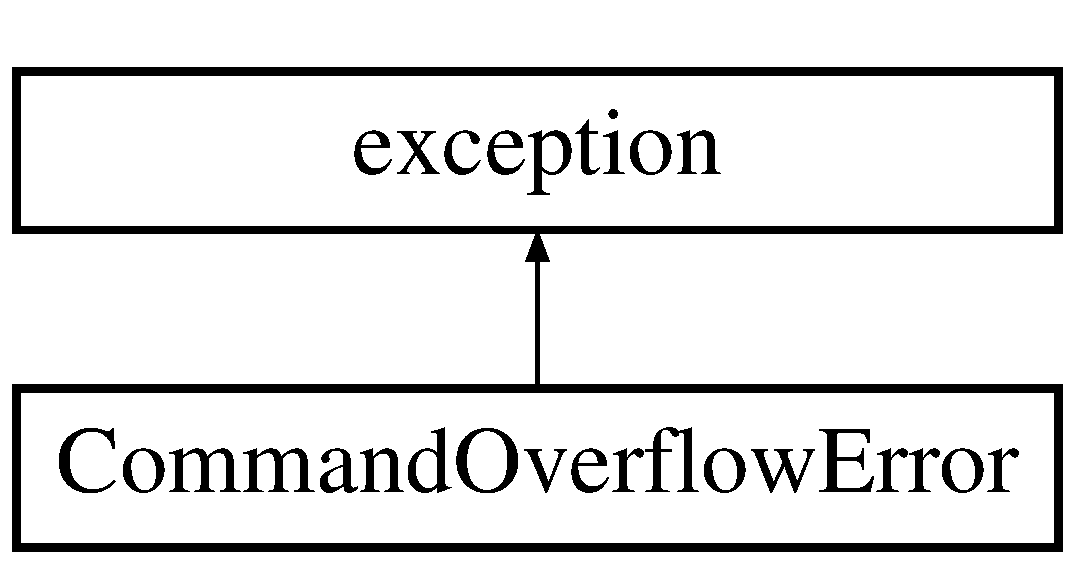
\includegraphics[height=2.000000cm]{class_command_overflow_error}
\end{center}
\end{figure}
\doxysubsection*{Открытые члены}
\begin{DoxyCompactItemize}
\item 
\mbox{\Hypertarget{class_command_overflow_error_abc1209a8ef74d20820d88d2384201089}\label{class_command_overflow_error_abc1209a8ef74d20820d88d2384201089}} 
{\bfseries Command\+Overflow\+Error} (const string \&error=\char`\"{}500 Command overflow error\char`\"{})
\item 
\mbox{\Hypertarget{class_command_overflow_error_a95abab220da5443ef5a2e0c478ea8733}\label{class_command_overflow_error_a95abab220da5443ef5a2e0c478ea8733}} 
const char $\ast$ {\bfseries what} () const noexcept override
\end{DoxyCompactItemize}


Объявления и описания членов класса находятся в файле\+:\begin{DoxyCompactItemize}
\item 
exceptions.\+h\end{DoxyCompactItemize}

\hypertarget{class_conflict}{}\doxysection{Класс Conflict}
\label{class_conflict}\index{Conflict@{Conflict}}
Граф наследования\+:Conflict\+:\begin{figure}[H]
\begin{center}
\leavevmode
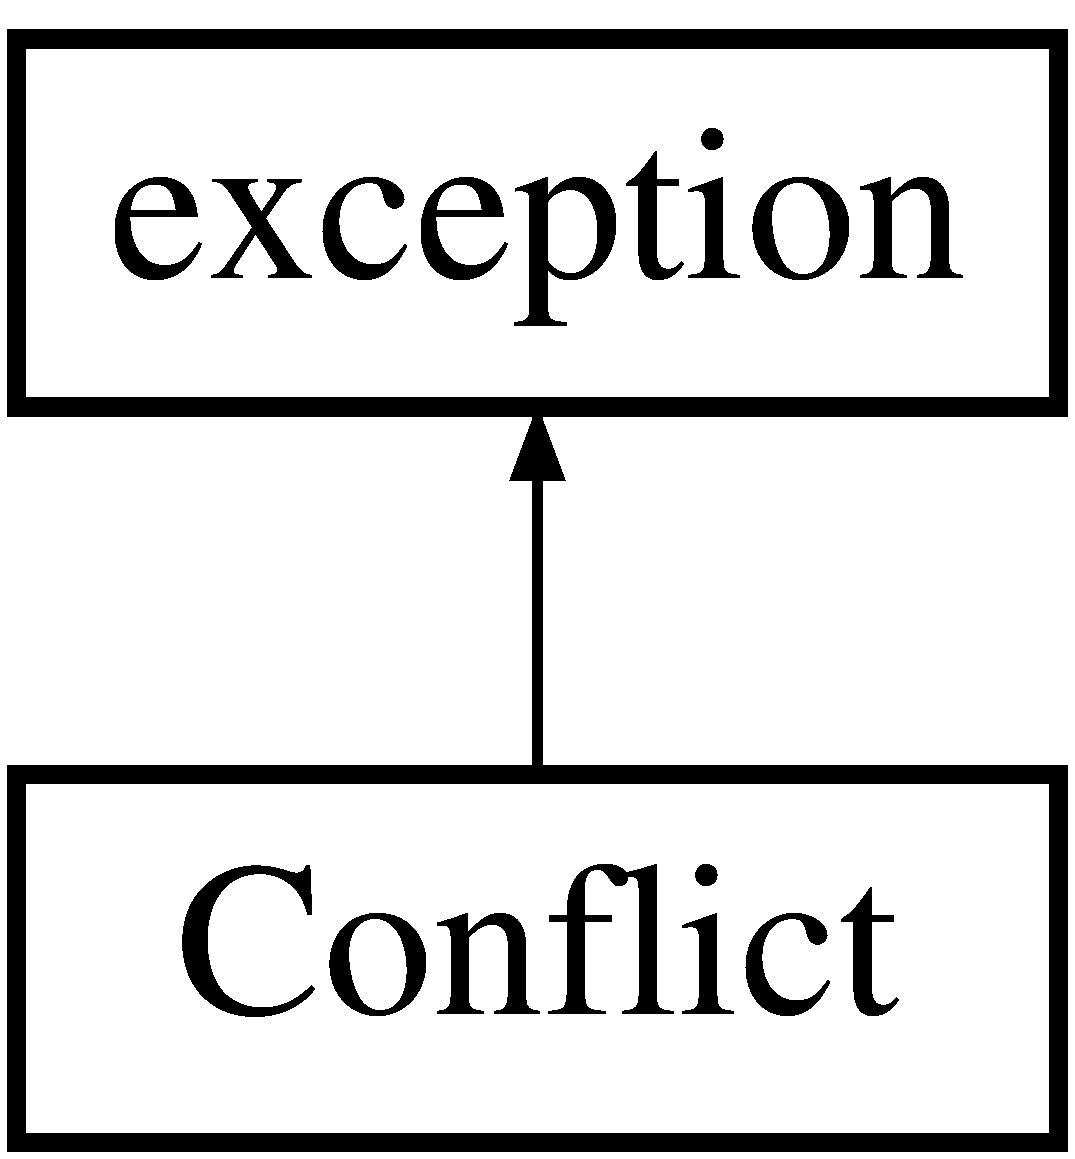
\includegraphics[height=2.000000cm]{class_conflict}
\end{center}
\end{figure}
\doxysubsection*{Открытые члены}
\begin{DoxyCompactItemize}
\item 
\mbox{\Hypertarget{class_conflict_a185c6c0b89dcdf1305e3cbf1555aa84d}\label{class_conflict_a185c6c0b89dcdf1305e3cbf1555aa84d}} 
{\bfseries Conflict} (const string \&error=\char`\"{}Conflict\char`\"{})
\item 
\mbox{\Hypertarget{class_conflict_ac09f74685507fdb4a40a3a507c7d339a}\label{class_conflict_ac09f74685507fdb4a40a3a507c7d339a}} 
const char $\ast$ {\bfseries what} () const noexcept override
\end{DoxyCompactItemize}


Объявления и описания членов класса находятся в файле\+:\begin{DoxyCompactItemize}
\item 
exceptions.\+h\end{DoxyCompactItemize}

\hypertarget{struct_s_p_u_1_1_fields_container_1_1_content_struct}{}\doxysection{Структура S\+PU\+::Fields\+Container$<$ NameT, ContentT $>$\+::Content\+Struct}
\label{struct_s_p_u_1_1_fields_container_1_1_content_struct}\index{SPU::FieldsContainer$<$ NameT, ContentT $>$::ContentStruct@{SPU::FieldsContainer$<$ NameT, ContentT $>$::ContentStruct}}
\doxysubsection*{Открытые члены}
\begin{DoxyCompactItemize}
\item 
\mbox{\Hypertarget{struct_s_p_u_1_1_fields_container_1_1_content_struct_ab6645fcbc525be9c8c75d07b58ab72d4}\label{struct_s_p_u_1_1_fields_container_1_1_content_struct_ab6645fcbc525be9c8c75d07b58ab72d4}} 
{\bfseries Content\+Struct} (NameT c\+\_\+name, ContentT c\+\_\+cont)
\end{DoxyCompactItemize}
\doxysubsection*{Открытые атрибуты}
\begin{DoxyCompactItemize}
\item 
\mbox{\Hypertarget{struct_s_p_u_1_1_fields_container_1_1_content_struct_a6d13eec3a77c6d5cbb41a11f3f15aa80}\label{struct_s_p_u_1_1_fields_container_1_1_content_struct_a6d13eec3a77c6d5cbb41a11f3f15aa80}} 
NameT {\bfseries name}
\item 
\mbox{\Hypertarget{struct_s_p_u_1_1_fields_container_1_1_content_struct_a298bb38a5cf283514b536ad0010740a4}\label{struct_s_p_u_1_1_fields_container_1_1_content_struct_a298bb38a5cf283514b536ad0010740a4}} 
\begin{tabbing}
xx\=xx\=xx\=xx\=xx\=xx\=xx\=xx\=xx\=\kill
union \{\\
\>ContentT {\bfseries cont}\\
\>ContentT {\bfseries data}\\
\>ContentT {\bfseries length}\\
\}; \\

\end{tabbing}\end{DoxyCompactItemize}


Объявления и описания членов структуры находятся в файле\+:\begin{DoxyCompactItemize}
\item 
spu-\/api/libspu/fields\+\_\+containers.\+hpp\end{DoxyCompactItemize}

\hypertarget{struct_s_p_u_1_1_could_not_create_structure}{}\section{Структура S\+PU\+:\+:Could\+Not\+Create\+Structure}
\label{struct_s_p_u_1_1_could_not_create_structure}\index{S\+P\+U\+::\+Could\+Not\+Create\+Structure@{S\+P\+U\+::\+Could\+Not\+Create\+Structure}}
Граф наследования\+:S\+PU\+:\+:Could\+Not\+Create\+Structure\+:\begin{figure}[H]
\begin{center}
\leavevmode
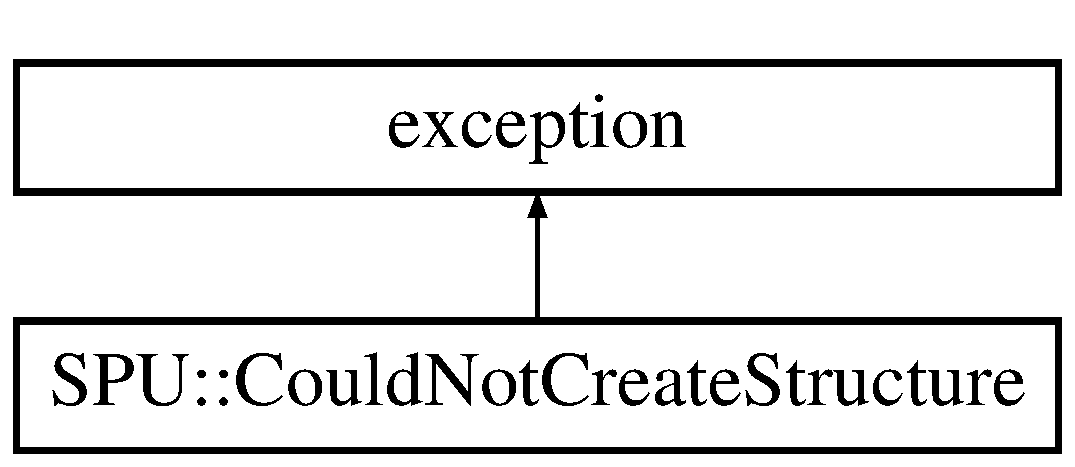
\includegraphics[height=2.000000cm]{struct_s_p_u_1_1_could_not_create_structure}
\end{center}
\end{figure}
\subsection*{Открытые члены}
\begin{DoxyCompactItemize}
\item 
\mbox{\Hypertarget{struct_s_p_u_1_1_could_not_create_structure_a7edb5a77f07de1db2b7e16f9370bb5f8}\label{struct_s_p_u_1_1_could_not_create_structure_a7edb5a77f07de1db2b7e16f9370bb5f8}} 
const char $\ast$ {\bfseries what} () const  throw ()
\end{DoxyCompactItemize}


Объявления и описания членов структуры находятся в файле\+:\begin{DoxyCompactItemize}
\item 
spu-\/api/libspu/errors/could\+\_\+not\+\_\+create\+\_\+structure.\+hpp\end{DoxyCompactItemize}

\hypertarget{structdata__container}{}\section{Структура data\+\_\+container}
\label{structdata__container}\index{data\+\_\+container@{data\+\_\+container}}
\subsection*{Открытые атрибуты}
\begin{DoxyCompactItemize}
\item 
\mbox{\Hypertarget{structdata__container_aca87ea9dd5d4263504c7743e770dcce3}\label{structdata__container_aca87ea9dd5d4263504c7743e770dcce3}} 
u32 {\bfseries cont} \mbox{[}S\+P\+U\+\_\+\+W\+E\+I\+G\+HT\mbox{]}
\end{DoxyCompactItemize}


Объявления и описания членов структуры находятся в файле\+:\begin{DoxyCompactItemize}
\item 
spu-\/api/libspu/spu.\+h\end{DoxyCompactItemize}

\hypertarget{struct_s_p_u_1_1_did_not_found_data_by_name}{}\doxysection{Шаблон структуры S\+PU\+::Did\+Not\+Found\+Data\+By\+Name$<$ NameT $>$}
\label{struct_s_p_u_1_1_did_not_found_data_by_name}\index{SPU::DidNotFoundDataByName$<$ NameT $>$@{SPU::DidNotFoundDataByName$<$ NameT $>$}}
Граф наследования\+:S\+PU\+::Did\+Not\+Found\+Data\+By\+Name$<$ NameT $>$\+:\begin{figure}[H]
\begin{center}
\leavevmode
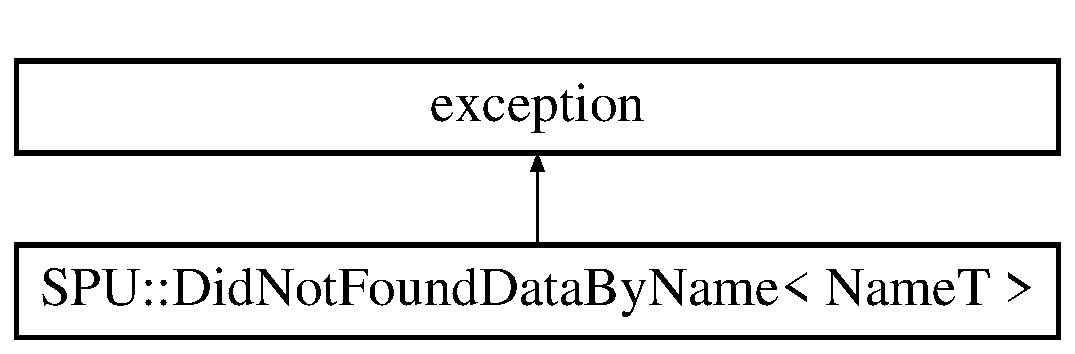
\includegraphics[height=2.000000cm]{struct_s_p_u_1_1_did_not_found_data_by_name}
\end{center}
\end{figure}
\doxysubsection*{Открытые члены}
\begin{DoxyCompactItemize}
\item 
\mbox{\Hypertarget{struct_s_p_u_1_1_did_not_found_data_by_name_a36425abe5ba033c069c704383870dd81}\label{struct_s_p_u_1_1_did_not_found_data_by_name_a36425abe5ba033c069c704383870dd81}} 
{\bfseries Did\+Not\+Found\+Data\+By\+Name} (std\+::string class\+\_\+name, NameT exception\+\_\+field\+\_\+name)
\item 
\mbox{\Hypertarget{struct_s_p_u_1_1_did_not_found_data_by_name_ac40019d6c1f692d2e2b7f56b4bf180ea}\label{struct_s_p_u_1_1_did_not_found_data_by_name_ac40019d6c1f692d2e2b7f56b4bf180ea}} 
std\+::string {\bfseries str\+\_\+what\+\_\+field\+\_\+name} (NameT exception\+\_\+field\+\_\+name)
\item 
\mbox{\Hypertarget{struct_s_p_u_1_1_did_not_found_data_by_name_ab31e718db83c43fd2d1688840224e62f}\label{struct_s_p_u_1_1_did_not_found_data_by_name_ab31e718db83c43fd2d1688840224e62f}} 
const char $\ast$ {\bfseries what} () const  throw ()
\item 
\mbox{\Hypertarget{struct_s_p_u_1_1_did_not_found_data_by_name_aa15a4a177de8c850e33af1e57c70cb23}\label{struct_s_p_u_1_1_did_not_found_data_by_name_aa15a4a177de8c850e33af1e57c70cb23}} 
std\+::string {\bfseries str\+\_\+what\+\_\+field\+\_\+name} (std\+::string exception\+\_\+field\+\_\+name)
\item 
\mbox{\Hypertarget{struct_s_p_u_1_1_did_not_found_data_by_name_a0a5121d73c3b99c49b295653952a4bca}\label{struct_s_p_u_1_1_did_not_found_data_by_name_a0a5121d73c3b99c49b295653952a4bca}} 
std\+::string {\bfseries str\+\_\+what\+\_\+field\+\_\+name} (char exception\+\_\+field\+\_\+name)
\item 
\mbox{\Hypertarget{struct_s_p_u_1_1_did_not_found_data_by_name_a9ad8708f0ca30c79c408c06e365e2492}\label{struct_s_p_u_1_1_did_not_found_data_by_name_a9ad8708f0ca30c79c408c06e365e2492}} 
std\+::string {\bfseries str\+\_\+what\+\_\+field\+\_\+name} (short exception\+\_\+field\+\_\+name)
\item 
\mbox{\Hypertarget{struct_s_p_u_1_1_did_not_found_data_by_name_af2698743aefdeb9270973fbb9b3484a9}\label{struct_s_p_u_1_1_did_not_found_data_by_name_af2698743aefdeb9270973fbb9b3484a9}} 
std\+::string {\bfseries str\+\_\+what\+\_\+field\+\_\+name} (int exception\+\_\+field\+\_\+name)
\item 
\mbox{\Hypertarget{struct_s_p_u_1_1_did_not_found_data_by_name_a4303843250c389719bb91b4d9d08ad2c}\label{struct_s_p_u_1_1_did_not_found_data_by_name_a4303843250c389719bb91b4d9d08ad2c}} 
std\+::string {\bfseries str\+\_\+what\+\_\+field\+\_\+name} (long exception\+\_\+field\+\_\+name)
\item 
\mbox{\Hypertarget{struct_s_p_u_1_1_did_not_found_data_by_name_a51c2096301a93a9811485226abefddab}\label{struct_s_p_u_1_1_did_not_found_data_by_name_a51c2096301a93a9811485226abefddab}} 
std\+::string {\bfseries str\+\_\+what\+\_\+field\+\_\+name} (long long exception\+\_\+field\+\_\+name)
\item 
\mbox{\Hypertarget{struct_s_p_u_1_1_did_not_found_data_by_name_a7aec2ef3d591ffef18fd68e675f26ff9}\label{struct_s_p_u_1_1_did_not_found_data_by_name_a7aec2ef3d591ffef18fd68e675f26ff9}} 
std\+::string {\bfseries str\+\_\+what\+\_\+field\+\_\+name} (unsigned char exception\+\_\+field\+\_\+name)
\item 
\mbox{\Hypertarget{struct_s_p_u_1_1_did_not_found_data_by_name_a334bb7c92362ccb88c7e0de8480f8192}\label{struct_s_p_u_1_1_did_not_found_data_by_name_a334bb7c92362ccb88c7e0de8480f8192}} 
std\+::string {\bfseries str\+\_\+what\+\_\+field\+\_\+name} (unsigned short exception\+\_\+field\+\_\+name)
\item 
\mbox{\Hypertarget{struct_s_p_u_1_1_did_not_found_data_by_name_acccc2ad2ed7d744a76650504ed1848ad}\label{struct_s_p_u_1_1_did_not_found_data_by_name_acccc2ad2ed7d744a76650504ed1848ad}} 
std\+::string {\bfseries str\+\_\+what\+\_\+field\+\_\+name} (unsigned int exception\+\_\+field\+\_\+name)
\item 
\mbox{\Hypertarget{struct_s_p_u_1_1_did_not_found_data_by_name_af8161beda0381022eaff0e60ba6107df}\label{struct_s_p_u_1_1_did_not_found_data_by_name_af8161beda0381022eaff0e60ba6107df}} 
std\+::string {\bfseries str\+\_\+what\+\_\+field\+\_\+name} (unsigned long exception\+\_\+field\+\_\+name)
\item 
\mbox{\Hypertarget{struct_s_p_u_1_1_did_not_found_data_by_name_ae015cc6f9287429604fefc6b99b9a0e5}\label{struct_s_p_u_1_1_did_not_found_data_by_name_ae015cc6f9287429604fefc6b99b9a0e5}} 
std\+::string {\bfseries str\+\_\+what\+\_\+field\+\_\+name} (unsigned long long exception\+\_\+field\+\_\+name)
\end{DoxyCompactItemize}
\doxysubsection*{Открытые атрибуты}
\begin{DoxyCompactItemize}
\item 
\mbox{\Hypertarget{struct_s_p_u_1_1_did_not_found_data_by_name_a7f80657f0a0fd12a4b7705d5128067bc}\label{struct_s_p_u_1_1_did_not_found_data_by_name_a7f80657f0a0fd12a4b7705d5128067bc}} 
std\+::string {\bfseries str\+\_\+what}
\end{DoxyCompactItemize}


Объявления и описания членов структуры находятся в файле\+:\begin{DoxyCompactItemize}
\item 
spu-\/api/libspu/errors/did\+\_\+not\+\_\+found\+\_\+by\+\_\+name.\+hpp\end{DoxyCompactItemize}

\hypertarget{classedge__property__writer}{}\section{Класс edge\+\_\+property\+\_\+writer}
\label{classedge__property__writer}\index{edge\+\_\+property\+\_\+writer@{edge\+\_\+property\+\_\+writer}}
\subsection*{Открытые члены}
\begin{DoxyCompactItemize}
\item 
\mbox{\Hypertarget{classedge__property__writer_acaadbf3e0c9e0e96847ecff5cd24af54}\label{classedge__property__writer_acaadbf3e0c9e0e96847ecff5cd24af54}} 
{\bfseries edge\+\_\+property\+\_\+writer} (\hyperlink{class_s_p_u___g_r_a_p_h_1_1_spu_ultra_graph}{Spu\+Ultra\+Graph} \&g)
\item 
\mbox{\Hypertarget{classedge__property__writer_a4a8ac776bd83aab3afb64cd3ed9e489c}\label{classedge__property__writer_a4a8ac776bd83aab3afb64cd3ed9e489c}} 
void {\bfseries operator()} (std\+::ostream \&out, const \hyperlink{class_s_p_u___g_r_a_p_h_1_1_spu_ultra_graph_a5f3776e003ef0a1648f1d9f84289810b}{Spu\+Ultra\+Graph\+::edge\+\_\+descriptor} \&e) const
\item 
\mbox{\Hypertarget{classedge__property__writer_acaadbf3e0c9e0e96847ecff5cd24af54}\label{classedge__property__writer_acaadbf3e0c9e0e96847ecff5cd24af54}} 
{\bfseries edge\+\_\+property\+\_\+writer} (\hyperlink{class_s_p_u___g_r_a_p_h_1_1_spu_ultra_graph}{Spu\+Ultra\+Graph} \&g)
\item 
\mbox{\Hypertarget{classedge__property__writer_a4a8ac776bd83aab3afb64cd3ed9e489c}\label{classedge__property__writer_a4a8ac776bd83aab3afb64cd3ed9e489c}} 
void {\bfseries operator()} (std\+::ostream \&out, const \hyperlink{class_s_p_u___g_r_a_p_h_1_1_spu_ultra_graph_a5f3776e003ef0a1648f1d9f84289810b}{Spu\+Ultra\+Graph\+::edge\+\_\+descriptor} \&e) const
\end{DoxyCompactItemize}


Объявления и описания членов классов находятся в файлах\+:\begin{DoxyCompactItemize}
\item 
examples/dijkstra\+\_\+example.\+cpp\item 
examples/graphvis\+\_\+example.\+cpp\end{DoxyCompactItemize}

\hypertarget{class_s_p_u___g_r_a_p_h_1_1_spu_ultra_graph_1_1_edge_iterator}{}\section{Класс S\+P\+U\+\_\+\+G\+R\+A\+PH\+:\+:Spu\+Ultra\+Graph\+:\+:Edge\+Iterator}
\label{class_s_p_u___g_r_a_p_h_1_1_spu_ultra_graph_1_1_edge_iterator}\index{S\+P\+U\+\_\+\+G\+R\+A\+P\+H\+::\+Spu\+Ultra\+Graph\+::\+Edge\+Iterator@{S\+P\+U\+\_\+\+G\+R\+A\+P\+H\+::\+Spu\+Ultra\+Graph\+::\+Edge\+Iterator}}
Граф наследования\+:S\+P\+U\+\_\+\+G\+R\+A\+PH\+:\+:Spu\+Ultra\+Graph\+:\+:Edge\+Iterator\+:\begin{figure}[H]
\begin{center}
\leavevmode
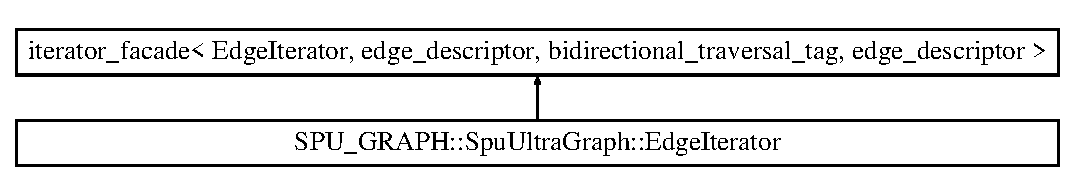
\includegraphics[height=2.000000cm]{class_s_p_u___g_r_a_p_h_1_1_spu_ultra_graph_1_1_edge_iterator}
\end{center}
\end{figure}
\subsection*{Открытые члены}
\begin{DoxyCompactItemize}
\item 
\mbox{\Hypertarget{class_s_p_u___g_r_a_p_h_1_1_spu_ultra_graph_1_1_edge_iterator_af258057cf189f894ba94bd0eb204ccf8}\label{class_s_p_u___g_r_a_p_h_1_1_spu_ultra_graph_1_1_edge_iterator_af258057cf189f894ba94bd0eb204ccf8}} 
{\bfseries Edge\+Iterator} (const \hyperlink{class_s_p_u___g_r_a_p_h_1_1_spu_ultra_graph}{Spu\+Ultra\+Graph} $\ast$g, \hyperlink{class_s_p_u___g_r_a_p_h_1_1_spu_ultra_graph_a5f3776e003ef0a1648f1d9f84289810b}{edge\+\_\+descriptor} \hyperlink{class_s_p_u___g_r_a_p_h_1_1_spu_ultra_graph_a51468aa2278d3abb0c338ffbeac7747a}{edge}=0)
\item 
\mbox{\Hypertarget{class_s_p_u___g_r_a_p_h_1_1_spu_ultra_graph_1_1_edge_iterator_a16b8fa40556388fcd34f1fc60875fcb7}\label{class_s_p_u___g_r_a_p_h_1_1_spu_ultra_graph_1_1_edge_iterator_a16b8fa40556388fcd34f1fc60875fcb7}} 
\hyperlink{class_s_p_u___g_r_a_p_h_1_1_spu_ultra_graph_a5f3776e003ef0a1648f1d9f84289810b}{edge\+\_\+descriptor} {\bfseries dereference} () const
\item 
\mbox{\Hypertarget{class_s_p_u___g_r_a_p_h_1_1_spu_ultra_graph_1_1_edge_iterator_aafe02491fd261530f0401712d10d42c2}\label{class_s_p_u___g_r_a_p_h_1_1_spu_ultra_graph_1_1_edge_iterator_aafe02491fd261530f0401712d10d42c2}} 
bool {\bfseries equal} (const \hyperlink{class_s_p_u___g_r_a_p_h_1_1_spu_ultra_graph_1_1_edge_iterator}{Edge\+Iterator} \&other) const
\item 
\mbox{\Hypertarget{class_s_p_u___g_r_a_p_h_1_1_spu_ultra_graph_1_1_edge_iterator_a6f6a205cfb0546d7a4063ae78a00ffaf}\label{class_s_p_u___g_r_a_p_h_1_1_spu_ultra_graph_1_1_edge_iterator_a6f6a205cfb0546d7a4063ae78a00ffaf}} 
void {\bfseries increment} ()
\item 
\mbox{\Hypertarget{class_s_p_u___g_r_a_p_h_1_1_spu_ultra_graph_1_1_edge_iterator_aabc6a676b6aa95ad845bf6bba49e2517}\label{class_s_p_u___g_r_a_p_h_1_1_spu_ultra_graph_1_1_edge_iterator_aabc6a676b6aa95ad845bf6bba49e2517}} 
void {\bfseries decrement} ()
\end{DoxyCompactItemize}
\subsection*{Друзья}
\begin{DoxyCompactItemize}
\item 
\mbox{\Hypertarget{class_s_p_u___g_r_a_p_h_1_1_spu_ultra_graph_1_1_edge_iterator_a0975271623c74c5b89bdf8d7fbce69c4}\label{class_s_p_u___g_r_a_p_h_1_1_spu_ultra_graph_1_1_edge_iterator_a0975271623c74c5b89bdf8d7fbce69c4}} 
class {\bfseries iterator\+\_\+core\+\_\+access}
\end{DoxyCompactItemize}


Объявления и описания членов классов находятся в файлах\+:\begin{DoxyCompactItemize}
\item 
Spu\+Ultra\+Graph.\+h\item 
Spu\+Ultra\+Graph.\+cpp\end{DoxyCompactItemize}

\hypertarget{class_s_p_u___g_r_a_p_h_1_1_spu_ultra_graph_1_1_edges}{}\doxysection{Класс S\+P\+U\+\_\+\+G\+R\+A\+PH\+::Spu\+Ultra\+Graph\+::Edges}
\label{class_s_p_u___g_r_a_p_h_1_1_spu_ultra_graph_1_1_edges}\index{SPU\_GRAPH::SpuUltraGraph::Edges@{SPU\_GRAPH::SpuUltraGraph::Edges}}


Контейнер содержащий все ребра графа  




{\ttfamily \#include $<$Spu\+Ultra\+Graph.\+h$>$}

\doxysubsection*{Открытые типы}
\begin{DoxyCompactItemize}
\item 
\mbox{\Hypertarget{class_s_p_u___g_r_a_p_h_1_1_spu_ultra_graph_1_1_edges_ac1ca1082fcec48528a49b2cbd2306892}\label{class_s_p_u___g_r_a_p_h_1_1_spu_ultra_graph_1_1_edges_ac1ca1082fcec48528a49b2cbd2306892}} 
typedef \mbox{\hyperlink{class_s_p_u___g_r_a_p_h_1_1_spu_ultra_graph_abf3933dd7a8c18410837fee58a8a8a10}{edge\+\_\+iterator}} {\bfseries iterator}
\end{DoxyCompactItemize}
\doxysubsection*{Открытые члены}
\begin{DoxyCompactItemize}
\item 
\mbox{\Hypertarget{class_s_p_u___g_r_a_p_h_1_1_spu_ultra_graph_1_1_edges_aeea766c667e0ccdce1c2bdccb0aa52d9}\label{class_s_p_u___g_r_a_p_h_1_1_spu_ultra_graph_1_1_edges_aeea766c667e0ccdce1c2bdccb0aa52d9}} 
{\bfseries Edges} (const \mbox{\hyperlink{class_s_p_u___g_r_a_p_h_1_1_spu_ultra_graph}{Spu\+Ultra\+Graph}} $\ast$g)
\item 
\mbox{\Hypertarget{class_s_p_u___g_r_a_p_h_1_1_spu_ultra_graph_1_1_edges_ae1d28a5b50f8d3a09f30fd5a15da8581}\label{class_s_p_u___g_r_a_p_h_1_1_spu_ultra_graph_1_1_edges_ae1d28a5b50f8d3a09f30fd5a15da8581}} 
\mbox{\hyperlink{class_s_p_u___g_r_a_p_h_1_1_spu_ultra_graph_1_1_edge_iterator}{iterator}} {\bfseries begin} ()
\item 
\mbox{\Hypertarget{class_s_p_u___g_r_a_p_h_1_1_spu_ultra_graph_1_1_edges_abc2cc6d2223e45627e6a9539f289af80}\label{class_s_p_u___g_r_a_p_h_1_1_spu_ultra_graph_1_1_edges_abc2cc6d2223e45627e6a9539f289af80}} 
\mbox{\hyperlink{class_s_p_u___g_r_a_p_h_1_1_spu_ultra_graph_1_1_edge_iterator}{iterator}} {\bfseries end} ()
\end{DoxyCompactItemize}


\doxysubsection{Подробное описание}
Контейнер содержащий все ребра графа 

Объявления и описания членов класса находятся в файле\+:\begin{DoxyCompactItemize}
\item 
Spu\+Ultra\+Graph.\+h\end{DoxyCompactItemize}

\hypertarget{class_s_p_u___g_r_a_p_h_1_1_spu_ultra_graph_1_1_edge_vertices}{}\doxysection{Шаблон класса S\+P\+U\+\_\+\+G\+R\+A\+PH\+::Spu\+Ultra\+Graph\+::Edge\+Vertices$<$ I $>$}
\label{class_s_p_u___g_r_a_p_h_1_1_spu_ultra_graph_1_1_edge_vertices}\index{SPU\_GRAPH::SpuUltraGraph::EdgeVertices$<$ I $>$@{SPU\_GRAPH::SpuUltraGraph::EdgeVertices$<$ I $>$}}


Контейнер содержащий все источники для ребра e.  




{\ttfamily \#include $<$Spu\+Ultra\+Graph.\+h$>$}

\doxysubsection*{Открытые типы}
\begin{DoxyCompactItemize}
\item 
\mbox{\Hypertarget{class_s_p_u___g_r_a_p_h_1_1_spu_ultra_graph_1_1_edge_vertices_a73c467cb9960883efec3d69ce0d294ab}\label{class_s_p_u___g_r_a_p_h_1_1_spu_ultra_graph_1_1_edge_vertices_a73c467cb9960883efec3d69ce0d294ab}} 
typedef \mbox{\hyperlink{class_s_p_u___g_r_a_p_h_1_1_spu_ultra_graph_1_1_edge_vertices_iterator}{Edge\+Vertices\+Iterator}}$<$ I $>$ {\bfseries iterator}
\end{DoxyCompactItemize}
\doxysubsection*{Открытые члены}
\begin{DoxyCompactItemize}
\item 
\mbox{\Hypertarget{class_s_p_u___g_r_a_p_h_1_1_spu_ultra_graph_1_1_edge_vertices_a5f46b2bd30b600f3ac84ff3af6804331}\label{class_s_p_u___g_r_a_p_h_1_1_spu_ultra_graph_1_1_edge_vertices_a5f46b2bd30b600f3ac84ff3af6804331}} 
{\bfseries Edge\+Vertices} (const \mbox{\hyperlink{class_s_p_u___g_r_a_p_h_1_1_spu_ultra_graph}{Spu\+Ultra\+Graph}} $\ast$g, \mbox{\hyperlink{class_s_p_u___g_r_a_p_h_1_1_spu_ultra_graph_a5f3776e003ef0a1648f1d9f84289810b}{Spu\+Ultra\+Graph\+::edge\+\_\+descriptor}} e)
\item 
\mbox{\Hypertarget{class_s_p_u___g_r_a_p_h_1_1_spu_ultra_graph_1_1_edge_vertices_a436d1084d81c01646f2ed88520909c16}\label{class_s_p_u___g_r_a_p_h_1_1_spu_ultra_graph_1_1_edge_vertices_a436d1084d81c01646f2ed88520909c16}} 
\mbox{\hyperlink{class_s_p_u___g_r_a_p_h_1_1_spu_ultra_graph_1_1_edge_vertices_iterator}{iterator}} {\bfseries begin} ()
\item 
\mbox{\Hypertarget{class_s_p_u___g_r_a_p_h_1_1_spu_ultra_graph_1_1_edge_vertices_ae3d69f0dca98f169ed2267a14dd81261}\label{class_s_p_u___g_r_a_p_h_1_1_spu_ultra_graph_1_1_edge_vertices_ae3d69f0dca98f169ed2267a14dd81261}} 
\mbox{\hyperlink{class_s_p_u___g_r_a_p_h_1_1_spu_ultra_graph_1_1_edge_vertices_iterator}{iterator}} {\bfseries end} ()
\item 
\mbox{\Hypertarget{class_s_p_u___g_r_a_p_h_1_1_spu_ultra_graph_1_1_edge_vertices_afc0ed5eee0521e7b83bfb25a604b5c88}\label{class_s_p_u___g_r_a_p_h_1_1_spu_ultra_graph_1_1_edge_vertices_afc0ed5eee0521e7b83bfb25a604b5c88}} 
\mbox{\hyperlink{class_s_p_u___g_r_a_p_h_1_1_spu_ultra_graph_1_1_edge_vertices_iterator}{iterator}} {\bfseries rbegin} ()
\item 
\mbox{\Hypertarget{class_s_p_u___g_r_a_p_h_1_1_spu_ultra_graph_1_1_edge_vertices_a3b2972bf4010a0585f3c7ceb0bb66620}\label{class_s_p_u___g_r_a_p_h_1_1_spu_ultra_graph_1_1_edge_vertices_a3b2972bf4010a0585f3c7ceb0bb66620}} 
\mbox{\hyperlink{class_s_p_u___g_r_a_p_h_1_1_spu_ultra_graph_1_1_edge_vertices_iterator}{iterator}} {\bfseries rend} ()
\end{DoxyCompactItemize}


\doxysubsection{Подробное описание}
\subsubsection*{template$<$int I$>$\newline
class S\+P\+U\+\_\+\+G\+R\+A\+P\+H\+::\+Spu\+Ultra\+Graph\+::\+Edge\+Vertices$<$ I $>$}

Контейнер содержащий все источники для ребра e. 

Объявления и описания членов класса находятся в файле\+:\begin{DoxyCompactItemize}
\item 
Spu\+Ultra\+Graph.\+h\end{DoxyCompactItemize}

\hypertarget{class_s_p_u___g_r_a_p_h_1_1_spu_ultra_graph_1_1_edge_vertices_iterator}{}\section{Шаблон класса S\+P\+U\+\_\+\+G\+R\+A\+PH\+:\+:Spu\+Ultra\+Graph\+:\+:Edge\+Vertices\+Iterator$<$ I $>$}
\label{class_s_p_u___g_r_a_p_h_1_1_spu_ultra_graph_1_1_edge_vertices_iterator}\index{S\+P\+U\+\_\+\+G\+R\+A\+P\+H\+::\+Spu\+Ultra\+Graph\+::\+Edge\+Vertices\+Iterator$<$ I $>$@{S\+P\+U\+\_\+\+G\+R\+A\+P\+H\+::\+Spu\+Ultra\+Graph\+::\+Edge\+Vertices\+Iterator$<$ I $>$}}


Итератор по смежным вершинам для ребра e.  




{\ttfamily \#include $<$Spu\+Ultra\+Graph.\+h$>$}

Граф наследования\+:S\+P\+U\+\_\+\+G\+R\+A\+PH\+:\+:Spu\+Ultra\+Graph\+:\+:Edge\+Vertices\+Iterator$<$ I $>$\+:\begin{figure}[H]
\begin{center}
\leavevmode
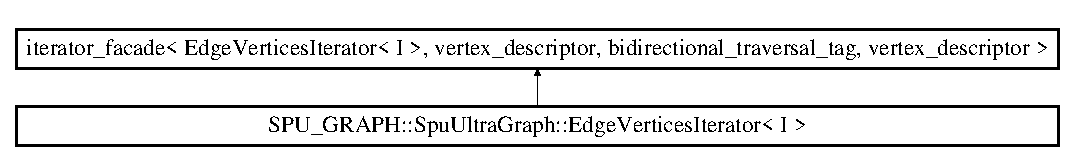
\includegraphics[height=1.728395cm]{class_s_p_u___g_r_a_p_h_1_1_spu_ultra_graph_1_1_edge_vertices_iterator}
\end{center}
\end{figure}
\subsection*{Открытые члены}
\begin{DoxyCompactItemize}
\item 
\mbox{\Hypertarget{class_s_p_u___g_r_a_p_h_1_1_spu_ultra_graph_1_1_edge_vertices_iterator_abfe6fdae2bd15033dc8003791fa3f80d}\label{class_s_p_u___g_r_a_p_h_1_1_spu_ultra_graph_1_1_edge_vertices_iterator_abfe6fdae2bd15033dc8003791fa3f80d}} 
{\bfseries Edge\+Vertices\+Iterator} (const \hyperlink{class_s_p_u___g_r_a_p_h_1_1_spu_ultra_graph}{Spu\+Ultra\+Graph} $\ast$g=nullptr, \hyperlink{class_s_p_u___g_r_a_p_h_1_1_spu_ultra_graph_a5f3776e003ef0a1648f1d9f84289810b}{edge\+\_\+descriptor} e=0, vertex\+\_\+descriptor v=0)
\item 
\mbox{\Hypertarget{class_s_p_u___g_r_a_p_h_1_1_spu_ultra_graph_1_1_edge_vertices_iterator_a8875d0fd54c7e8619acfd02bcb87d558}\label{class_s_p_u___g_r_a_p_h_1_1_spu_ultra_graph_1_1_edge_vertices_iterator_a8875d0fd54c7e8619acfd02bcb87d558}} 
vertex\+\_\+descriptor {\bfseries dereference} () const
\item 
\mbox{\Hypertarget{class_s_p_u___g_r_a_p_h_1_1_spu_ultra_graph_1_1_edge_vertices_iterator_ad165a565fb26b4fcd46a30a80fc457bb}\label{class_s_p_u___g_r_a_p_h_1_1_spu_ultra_graph_1_1_edge_vertices_iterator_ad165a565fb26b4fcd46a30a80fc457bb}} 
bool {\bfseries equal} (const \hyperlink{class_s_p_u___g_r_a_p_h_1_1_spu_ultra_graph_1_1_edge_vertices_iterator}{Edge\+Vertices\+Iterator}$<$ I $>$ \&other) const
\item 
\mbox{\Hypertarget{class_s_p_u___g_r_a_p_h_1_1_spu_ultra_graph_1_1_edge_vertices_iterator_a02101f156a9ff9d781a908df52bf32d0}\label{class_s_p_u___g_r_a_p_h_1_1_spu_ultra_graph_1_1_edge_vertices_iterator_a02101f156a9ff9d781a908df52bf32d0}} 
void {\bfseries increment} ()
\item 
\mbox{\Hypertarget{class_s_p_u___g_r_a_p_h_1_1_spu_ultra_graph_1_1_edge_vertices_iterator_a19530f355f4156c36d5e0e302c696662}\label{class_s_p_u___g_r_a_p_h_1_1_spu_ultra_graph_1_1_edge_vertices_iterator_a19530f355f4156c36d5e0e302c696662}} 
void {\bfseries decrement} ()
\end{DoxyCompactItemize}
\subsection*{Друзья}
\begin{DoxyCompactItemize}
\item 
\mbox{\Hypertarget{class_s_p_u___g_r_a_p_h_1_1_spu_ultra_graph_1_1_edge_vertices_iterator_a0975271623c74c5b89bdf8d7fbce69c4}\label{class_s_p_u___g_r_a_p_h_1_1_spu_ultra_graph_1_1_edge_vertices_iterator_a0975271623c74c5b89bdf8d7fbce69c4}} 
class {\bfseries iterator\+\_\+core\+\_\+access}
\end{DoxyCompactItemize}


\subsection{Подробное описание}
\subsubsection*{template$<$int I$>$\newline
class S\+P\+U\+\_\+\+G\+R\+A\+P\+H\+::\+Spu\+Ultra\+Graph\+::\+Edge\+Vertices\+Iterator$<$ I $>$}

Итератор по смежным вершинам для ребра e. 

Объявления и описания членов класса находятся в файле\+:\begin{DoxyCompactItemize}
\item 
Spu\+Ultra\+Graph.\+h\end{DoxyCompactItemize}

\hypertarget{class_s_p_u_1_1_extern_value}{}\doxysection{Шаблон класса S\+PU\+::Extern\+Value$<$ T $>$}
\label{class_s_p_u_1_1_extern_value}\index{SPU::ExternValue$<$ T $>$@{SPU::ExternValue$<$ T $>$}}
Граф наследования\+:S\+PU\+::Extern\+Value$<$ T $>$\+:\begin{figure}[H]
\begin{center}
\leavevmode
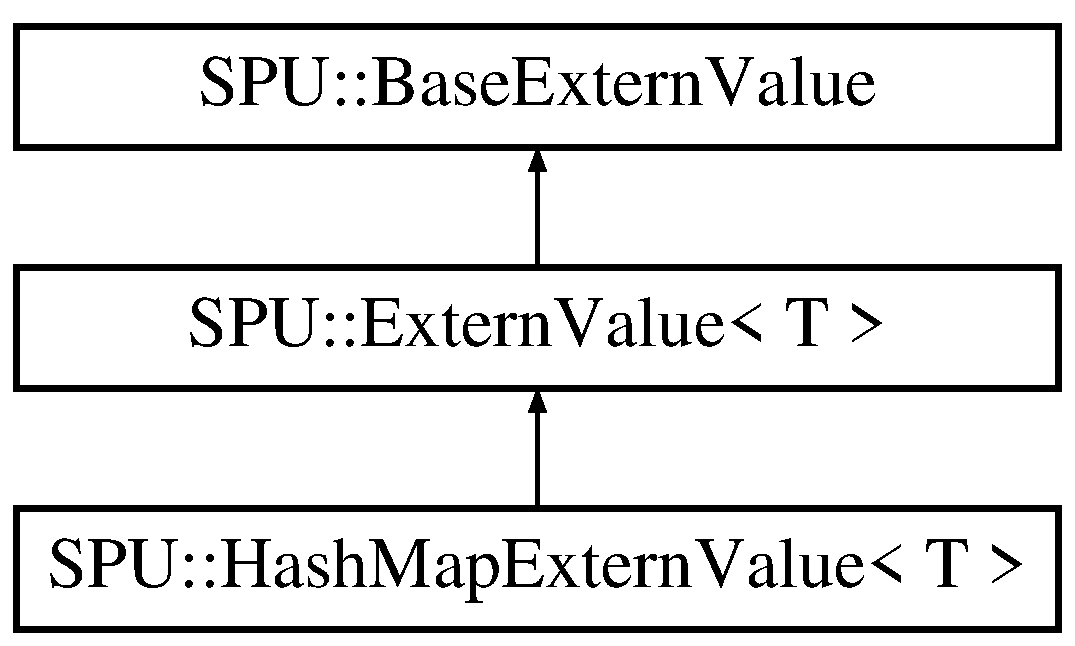
\includegraphics[height=3.000000cm]{class_s_p_u_1_1_extern_value}
\end{center}
\end{figure}
\doxysubsection*{Открытые члены}
\begin{DoxyCompactItemize}
\item 
\mbox{\Hypertarget{class_s_p_u_1_1_extern_value_aae7c6b4abbca7304d954311c58f32f4d}\label{class_s_p_u_1_1_extern_value_aae7c6b4abbca7304d954311c58f32f4d}} 
{\bfseries Extern\+Value} (value\+\_\+t id)
\item 
\mbox{\Hypertarget{class_s_p_u_1_1_extern_value_a8d8b98b83b4258cb2f5df76ffb10b4e0}\label{class_s_p_u_1_1_extern_value_a8d8b98b83b4258cb2f5df76ffb10b4e0}} 
virtual T \& {\bfseries get} ()=0
\item 
\mbox{\Hypertarget{class_s_p_u_1_1_extern_value_a4f55910a34f9de7442f5517a0bb2cce2}\label{class_s_p_u_1_1_extern_value_a4f55910a34f9de7442f5517a0bb2cce2}} 
virtual void {\bfseries set} (T value)=0
\item 
\mbox{\Hypertarget{class_s_p_u_1_1_extern_value_a6dc813c5d3721e291dea8586626c5319}\label{class_s_p_u_1_1_extern_value_a6dc813c5d3721e291dea8586626c5319}} 
{\bfseries operator T} ()
\item 
\mbox{\Hypertarget{class_s_p_u_1_1_extern_value_a62b3eb77df1467e81933dd6b3c6226a9}\label{class_s_p_u_1_1_extern_value_a62b3eb77df1467e81933dd6b3c6226a9}} 
\mbox{\hyperlink{class_s_p_u_1_1_extern_value}{Extern\+Value}} \& {\bfseries operator$<$$<$} (value\+\_\+t id)
\item 
\mbox{\Hypertarget{class_s_p_u_1_1_extern_value_a2757fc6516ddbd1bf072cfafc98fd6fc}\label{class_s_p_u_1_1_extern_value_a2757fc6516ddbd1bf072cfafc98fd6fc}} 
\mbox{\hyperlink{class_s_p_u_1_1_extern_value}{Extern\+Value}} \& {\bfseries operator$<$$<$} (\mbox{\hyperlink{struct_s_p_u_1_1pair__containter}{pair\+\_\+t}} pair)
\item 
\mbox{\Hypertarget{class_s_p_u_1_1_extern_value_aebe4ab28ad7d22c38aa622df2dbbe142}\label{class_s_p_u_1_1_extern_value_aebe4ab28ad7d22c38aa622df2dbbe142}} 
\mbox{\hyperlink{class_s_p_u_1_1_extern_value}{Extern\+Value}} \& {\bfseries operator$<$$<$} (T value)
\item 
\mbox{\Hypertarget{class_s_p_u_1_1_extern_value_acbb2ab9a89ce0d56f1bdafe8f0b9b796}\label{class_s_p_u_1_1_extern_value_acbb2ab9a89ce0d56f1bdafe8f0b9b796}} 
T \& {\bfseries operator$>$$>$} (T value)
\end{DoxyCompactItemize}
\doxysubsection*{Дополнительные унаследованные члены}


Объявления и описания членов класса находятся в файле\+:\begin{DoxyCompactItemize}
\item 
spu-\/api/libspu/extern\+\_\+value.\+hpp\end{DoxyCompactItemize}

\hypertarget{class_s_p_u_1_1_fields}{}\section{Шаблон класса S\+PU\+:\+:Fields$<$ NameT $>$}
\label{class_s_p_u_1_1_fields}\index{S\+P\+U\+::\+Fields$<$ Name\+T $>$@{S\+P\+U\+::\+Fields$<$ Name\+T $>$}}
Граф наследования\+:S\+PU\+:\+:Fields$<$ NameT $>$\+:\begin{figure}[H]
\begin{center}
\leavevmode
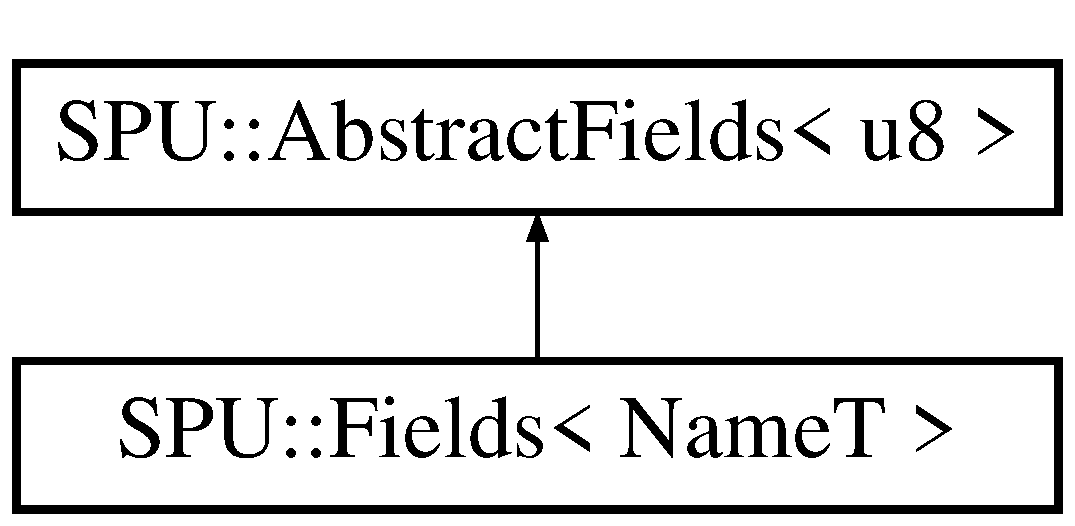
\includegraphics[height=2.000000cm]{class_s_p_u_1_1_fields}
\end{center}
\end{figure}
\subsection*{Открытые члены}
\begin{DoxyCompactItemize}
\item 
\mbox{\Hypertarget{class_s_p_u_1_1_fields_ae46e793567ed2f98bf3d2e9ce3960e16}\label{class_s_p_u_1_1_fields_ae46e793567ed2f98bf3d2e9ce3960e16}} 
{\bfseries Fields} (Length fields\+\_\+length)
\item 
\mbox{\Hypertarget{class_s_p_u_1_1_fields_ac2b4341d75532e5436232217ebac0116}\label{class_s_p_u_1_1_fields_ac2b4341d75532e5436232217ebac0116}} 
{\bfseries operator data\+\_\+t} () override
\item 
\mbox{\Hypertarget{class_s_p_u_1_1_fields_abfb59ae69298a677e4aeaa074b6d6341}\label{class_s_p_u_1_1_fields_abfb59ae69298a677e4aeaa074b6d6341}} 
\hyperlink{class_s_p_u_1_1_fields}{Fields} \& {\bfseries operator=} (data\+\_\+t fields\+\_\+data) override
\item 
\mbox{\Hypertarget{class_s_p_u_1_1_fields_a164f89e212b04114d390907dbdf8f3cf}\label{class_s_p_u_1_1_fields_a164f89e212b04114d390907dbdf8f3cf}} 
\hyperlink{class_s_p_u_1_1_fields}{Fields} \& {\bfseries operator=} (Data fields\+\_\+data) override
\item 
\mbox{\Hypertarget{class_s_p_u_1_1_fields_aba5505222d3f0d1befb223f778d3f070}\label{class_s_p_u_1_1_fields_aba5505222d3f0d1befb223f778d3f070}} 
data\+\_\+t \& {\bfseries operator\mbox{[}$\,$\mbox{]}} (NameT name) override
\end{DoxyCompactItemize}
\subsection*{Друзья}
\begin{DoxyCompactItemize}
\item 
\mbox{\Hypertarget{class_s_p_u_1_1_fields_aae763230135b011d2ac87be7970d9766}\label{class_s_p_u_1_1_fields_aae763230135b011d2ac87be7970d9766}} 
auto {\bfseries begin} (\hyperlink{class_s_p_u_1_1_fields}{Fields}$<$ NameT $>$ \&fields)
\item 
\mbox{\Hypertarget{class_s_p_u_1_1_fields_a0f39af32a7d42af30295d17d5e202692}\label{class_s_p_u_1_1_fields_a0f39af32a7d42af30295d17d5e202692}} 
auto {\bfseries end} (\hyperlink{class_s_p_u_1_1_fields}{Fields}$<$ NameT $>$ \&fields)
\end{DoxyCompactItemize}
\subsection*{Дополнительные унаследованные члены}


Объявления и описания членов класса находятся в файле\+:\begin{DoxyCompactItemize}
\item 
spu-\/api/libspu/fields.\+hpp\end{DoxyCompactItemize}

\hypertarget{class_s_p_u_1_1_fields_3_01void_01_4}{}\section{Шаблон класса S\+PU\+:\+:Fields$<$ void $>$}
\label{class_s_p_u_1_1_fields_3_01void_01_4}\index{S\+P\+U\+::\+Fields$<$ void $>$@{S\+P\+U\+::\+Fields$<$ void $>$}}
Граф наследования\+:S\+PU\+:\+:Fields$<$ void $>$\+:\begin{figure}[H]
\begin{center}
\leavevmode
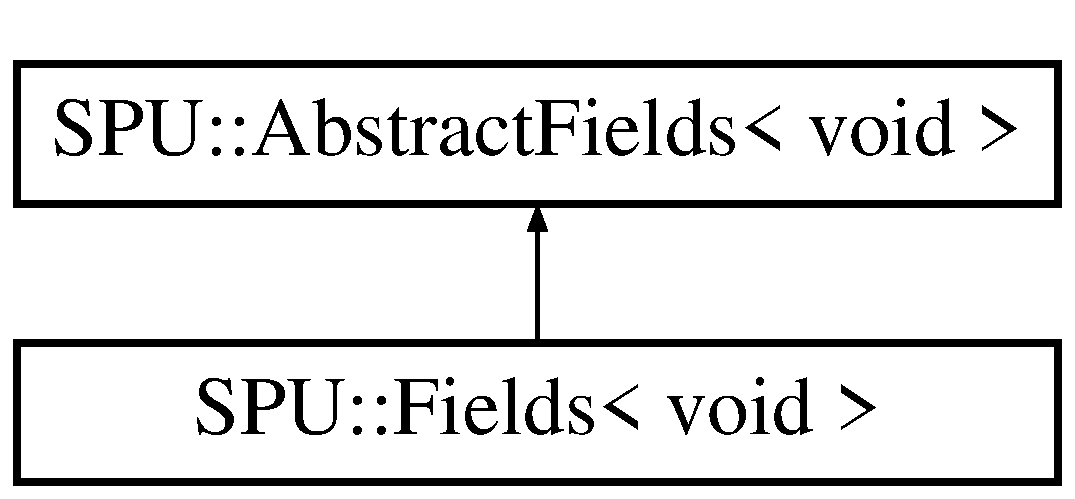
\includegraphics[height=2.000000cm]{class_s_p_u_1_1_fields_3_01void_01_4}
\end{center}
\end{figure}


Объявления и описания членов класса находятся в файле\+:\begin{DoxyCompactItemize}
\item 
spu-\/api/libspu/fields.\+hpp\end{DoxyCompactItemize}

\hypertarget{class_s_p_u_1_1_fields_container}{}\section{Шаблон класса S\+PU\+:\+:Fields\+Container$<$ NameT, ContentT $>$}
\label{class_s_p_u_1_1_fields_container}\index{S\+P\+U\+::\+Fields\+Container$<$ Name\+T, Content\+T $>$@{S\+P\+U\+::\+Fields\+Container$<$ Name\+T, Content\+T $>$}}
\subsection*{Классы}
\begin{DoxyCompactItemize}
\item 
struct \hyperlink{struct_s_p_u_1_1_fields_container_1_1_content_struct}{Content\+Struct}
\end{DoxyCompactItemize}
\subsection*{Открытые члены}
\begin{DoxyCompactItemize}
\item 
\mbox{\Hypertarget{class_s_p_u_1_1_fields_container_a53cf876b033420234d132395597eda7b}\label{class_s_p_u_1_1_fields_container_a53cf876b033420234d132395597eda7b}} 
{\bfseries Fields\+Container} (std\+::string Class\+Name)
\item 
\mbox{\Hypertarget{class_s_p_u_1_1_fields_container_aa3d1f42625ef5c8f4f6440f4c4df4eff}\label{class_s_p_u_1_1_fields_container_aa3d1f42625ef5c8f4f6440f4c4df4eff}} 
{\bfseries Fields\+Container} (Content\+Vector content\+\_\+vector, std\+::string Class\+Name)
\item 
\mbox{\Hypertarget{class_s_p_u_1_1_fields_container_a78bfa78d1c48cf6659552a36354f751d}\label{class_s_p_u_1_1_fields_container_a78bfa78d1c48cf6659552a36354f751d}} 
{\bfseries Fields\+Container} (std\+::initializer\+\_\+list$<$ \hyperlink{struct_s_p_u_1_1_fields_container_1_1_content_struct}{Content\+Struct} $>$ content\+\_\+initializer\+\_\+list, std\+::string Class\+Name)
\end{DoxyCompactItemize}
\subsection*{Защищенные типы}
\begin{DoxyCompactItemize}
\item 
\mbox{\Hypertarget{class_s_p_u_1_1_fields_container_ad1bff37d859918d4a7552d78fd7d3a30}\label{class_s_p_u_1_1_fields_container_ad1bff37d859918d4a7552d78fd7d3a30}} 
using {\bfseries Content\+Vector} = std\+::vector$<$ \hyperlink{struct_s_p_u_1_1_fields_container_1_1_content_struct}{Content\+Struct} $>$
\end{DoxyCompactItemize}
\subsection*{Защищенные члены}
\begin{DoxyCompactItemize}
\item 
\mbox{\Hypertarget{class_s_p_u_1_1_fields_container_a7ecfe5c05efc0ab4aee85e7f310275d3}\label{class_s_p_u_1_1_fields_container_a7ecfe5c05efc0ab4aee85e7f310275d3}} 
ContentT \& {\bfseries find\+\_\+data\+\_\+by\+\_\+name} (NameT name)
\item 
\mbox{\Hypertarget{class_s_p_u_1_1_fields_container_abbd05a1dba8a9275511ea9d4c4324c0b}\label{class_s_p_u_1_1_fields_container_abbd05a1dba8a9275511ea9d4c4324c0b}} 
const ContentT \& {\bfseries find\+\_\+data\+\_\+by\+\_\+name} (NameT name) const
\item 
\mbox{\Hypertarget{class_s_p_u_1_1_fields_container_acb3ab5dd1ac9d06eacf7617ddcfa1a58}\label{class_s_p_u_1_1_fields_container_acb3ab5dd1ac9d06eacf7617ddcfa1a58}} 
void {\bfseries push} (\hyperlink{struct_s_p_u_1_1_fields_container_1_1_content_struct}{Content\+Struct} addict)
\item 
\mbox{\Hypertarget{class_s_p_u_1_1_fields_container_a3bd09bbeaaa1d4c53f1ae730f10ccdc6}\label{class_s_p_u_1_1_fields_container_a3bd09bbeaaa1d4c53f1ae730f10ccdc6}} 
void {\bfseries clear} ()
\end{DoxyCompactItemize}
\subsection*{Друзья}
\begin{DoxyCompactItemize}
\item 
\mbox{\Hypertarget{class_s_p_u_1_1_fields_container_a34f7de31816f657140980e92f9299322}\label{class_s_p_u_1_1_fields_container_a34f7de31816f657140980e92f9299322}} 
auto {\bfseries begin} (\hyperlink{class_s_p_u_1_1_fields_container}{Fields\+Container}$<$ NameT, ContentT $>$ \&container)
\item 
\mbox{\Hypertarget{class_s_p_u_1_1_fields_container_a2e393ae5350f95f64be0cec98dfa95e9}\label{class_s_p_u_1_1_fields_container_a2e393ae5350f95f64be0cec98dfa95e9}} 
auto {\bfseries end} (\hyperlink{class_s_p_u_1_1_fields_container}{Fields\+Container}$<$ NameT, ContentT $>$ \&container)
\end{DoxyCompactItemize}


Объявления и описания членов класса находятся в файле\+:\begin{DoxyCompactItemize}
\item 
spu-\/api/libspu/fields\+\_\+containers.\+hpp\end{DoxyCompactItemize}

\hypertarget{class_s_p_u_1_1_fields_data}{}\section{Шаблон класса S\+PU\+:\+:Fields\+Data$<$ NameT $>$}
\label{class_s_p_u_1_1_fields_data}\index{S\+P\+U\+::\+Fields\+Data$<$ Name\+T $>$@{S\+P\+U\+::\+Fields\+Data$<$ Name\+T $>$}}
Граф наследования\+:S\+PU\+:\+:Fields\+Data$<$ NameT $>$\+:\begin{figure}[H]
\begin{center}
\leavevmode
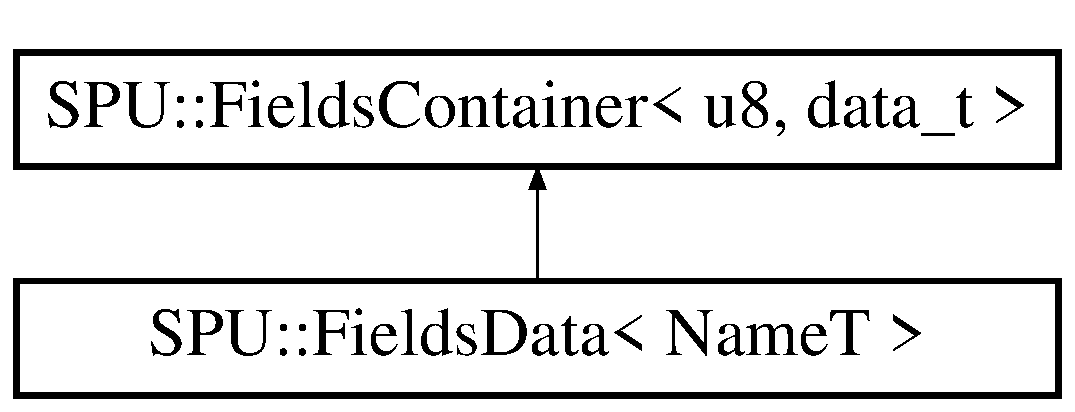
\includegraphics[height=2.000000cm]{class_s_p_u_1_1_fields_data}
\end{center}
\end{figure}
\subsection*{Открытые члены}
\begin{DoxyCompactItemize}
\item 
\mbox{\Hypertarget{class_s_p_u_1_1_fields_data_af5172a9b8709116bb462e23d10364073}\label{class_s_p_u_1_1_fields_data_af5172a9b8709116bb462e23d10364073}} 
{\bfseries Fields\+Data} (Data\+Vector data\+\_\+vector)
\item 
\mbox{\Hypertarget{class_s_p_u_1_1_fields_data_adb00b20681dd5a4142c47fc2386be31b}\label{class_s_p_u_1_1_fields_data_adb00b20681dd5a4142c47fc2386be31b}} 
{\bfseries Fields\+Data} (std\+::initializer\+\_\+list$<$ Data\+Struct $>$ data\+\_\+initializer\+\_\+list)
\item 
\mbox{\Hypertarget{class_s_p_u_1_1_fields_data_ae5b05f68095703c025a0a0fdfa3d1551}\label{class_s_p_u_1_1_fields_data_ae5b05f68095703c025a0a0fdfa3d1551}} 
void {\bfseries push} (Data\+Struct addict)
\item 
\mbox{\Hypertarget{class_s_p_u_1_1_fields_data_a11e983c717748422fec0e0f20e9e261a}\label{class_s_p_u_1_1_fields_data_a11e983c717748422fec0e0f20e9e261a}} 
void {\bfseries clear} ()
\item 
\mbox{\Hypertarget{class_s_p_u_1_1_fields_data_a1e1ec859160534ae5a52654295cf609a}\label{class_s_p_u_1_1_fields_data_a1e1ec859160534ae5a52654295cf609a}} 
const data\+\_\+t \& {\bfseries operator\mbox{[}$\,$\mbox{]}} (NameT name) const
\item 
\mbox{\Hypertarget{class_s_p_u_1_1_fields_data_a75a20498b05f5e29f8834878b0c080cf}\label{class_s_p_u_1_1_fields_data_a75a20498b05f5e29f8834878b0c080cf}} 
data\+\_\+t \& {\bfseries operator\mbox{[}$\,$\mbox{]}} (NameT name)
\end{DoxyCompactItemize}
\subsection*{Дополнительные унаследованные члены}


Объявления и описания членов класса находятся в файле\+:\begin{DoxyCompactItemize}
\item 
spu-\/api/libspu/fields\+\_\+containers.\+hpp\end{DoxyCompactItemize}

\hypertarget{class_s_p_u_1_1_fields_data_3_01void_01_4}{}\section{Шаблон класса S\+PU\+:\+:Fields\+Data$<$ void $>$}
\label{class_s_p_u_1_1_fields_data_3_01void_01_4}\index{S\+P\+U\+::\+Fields\+Data$<$ void $>$@{S\+P\+U\+::\+Fields\+Data$<$ void $>$}}


Объявления и описания членов класса находятся в файле\+:\begin{DoxyCompactItemize}
\item 
spu-\/api/libspu/fields\+\_\+containers.\+hpp\end{DoxyCompactItemize}

\hypertarget{class_s_p_u_1_1_fields_length}{}\doxysection{Шаблон класса S\+PU\+::Fields\+Length$<$ NameT $>$}
\label{class_s_p_u_1_1_fields_length}\index{SPU::FieldsLength$<$ NameT $>$@{SPU::FieldsLength$<$ NameT $>$}}
Граф наследования\+:S\+PU\+::Fields\+Length$<$ NameT $>$\+:\begin{figure}[H]
\begin{center}
\leavevmode
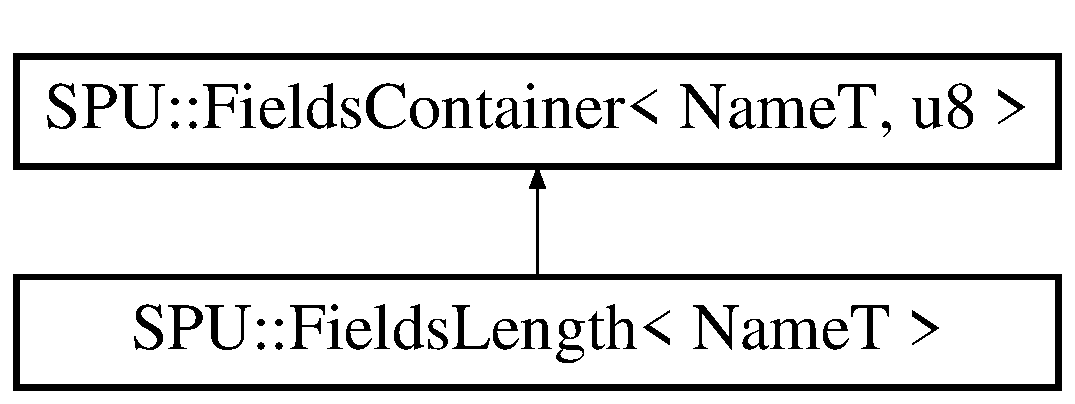
\includegraphics[height=2.000000cm]{class_s_p_u_1_1_fields_length}
\end{center}
\end{figure}
\doxysubsection*{Открытые типы}
\begin{DoxyCompactItemize}
\item 
\mbox{\Hypertarget{class_s_p_u_1_1_fields_length_af4bea5ce47fb204a757126230fb909c4}\label{class_s_p_u_1_1_fields_length_af4bea5ce47fb204a757126230fb909c4}} 
using {\bfseries Length\+Struct} = typename \mbox{\hyperlink{struct_s_p_u_1_1_fields_container_1_1_content_struct}{Parent\+::\+Content\+Struct}}
\item 
\mbox{\Hypertarget{class_s_p_u_1_1_fields_length_a2cb4735c3795ae52d6756fbd922c14e6}\label{class_s_p_u_1_1_fields_length_a2cb4735c3795ae52d6756fbd922c14e6}} 
using {\bfseries Length\+Vector} = typename Parent\+::\+Content\+Vector
\end{DoxyCompactItemize}
\doxysubsection*{Открытые члены}
\begin{DoxyCompactItemize}
\item 
\mbox{\Hypertarget{class_s_p_u_1_1_fields_length_a6c872b2d70d351407f6c935a3f1054c3}\label{class_s_p_u_1_1_fields_length_a6c872b2d70d351407f6c935a3f1054c3}} 
{\bfseries Fields\+Length} (Length\+Vector length\+\_\+vector)
\item 
\mbox{\Hypertarget{class_s_p_u_1_1_fields_length_a448add7e3c528c6f19cd55d5923b9235}\label{class_s_p_u_1_1_fields_length_a448add7e3c528c6f19cd55d5923b9235}} 
{\bfseries Fields\+Length} (std\+::initializer\+\_\+list$<$ Length\+Struct $>$ length\+\_\+initializer\+\_\+list)
\item 
\mbox{\Hypertarget{class_s_p_u_1_1_fields_length_a33dbec3b34b475fcf1afaba4155e3bf0}\label{class_s_p_u_1_1_fields_length_a33dbec3b34b475fcf1afaba4155e3bf0}} 
data\+\_\+t {\bfseries field\+Mask} (NameT name) const
\item 
\mbox{\Hypertarget{class_s_p_u_1_1_fields_length_a5dd2589e4576c96761f179b43f30869c}\label{class_s_p_u_1_1_fields_length_a5dd2589e4576c96761f179b43f30869c}} 
const u8 \& {\bfseries operator\mbox{[}$\,$\mbox{]}} (NameT name) const
\item 
\mbox{\Hypertarget{class_s_p_u_1_1_fields_length_a0fec8a15a660459656f4992ef56a03fe}\label{class_s_p_u_1_1_fields_length_a0fec8a15a660459656f4992ef56a03fe}} 
u8 \& {\bfseries operator\mbox{[}$\,$\mbox{]}} (NameT name)
\end{DoxyCompactItemize}
\doxysubsection*{Открытые статические члены}
\begin{DoxyCompactItemize}
\item 
\mbox{\Hypertarget{class_s_p_u_1_1_fields_length_a00ee369bbe966a9274289196e1d382b8}\label{class_s_p_u_1_1_fields_length_a00ee369bbe966a9274289196e1d382b8}} 
static data\+\_\+t {\bfseries mask} (u8 length)
\end{DoxyCompactItemize}
\doxysubsection*{Дополнительные унаследованные члены}


Объявления и описания членов класса находятся в файле\+:\begin{DoxyCompactItemize}
\item 
spu-\/api/libspu/fields\+\_\+containers.\+hpp\end{DoxyCompactItemize}

\hypertarget{class_s_p_u_1_1_fields_length_3_01void_01_4}{}\doxysection{Класс S\+PU\+::Fields\+Length$<$ void $>$}
\label{class_s_p_u_1_1_fields_length_3_01void_01_4}\index{SPU::FieldsLength$<$ void $>$@{SPU::FieldsLength$<$ void $>$}}


Объявления и описания членов класса находятся в файле\+:\begin{DoxyCompactItemize}
\item 
spu-\/api/libspu/fields\+\_\+containers.\+hpp\end{DoxyCompactItemize}

\hypertarget{class_s_p_u_1_1_fields_pointer}{}\doxysection{Шаблон класса S\+PU\+::Fields\+Pointer$<$ NameT $>$}
\label{class_s_p_u_1_1_fields_pointer}\index{SPU::FieldsPointer$<$ NameT $>$@{SPU::FieldsPointer$<$ NameT $>$}}
Граф наследования\+:S\+PU\+::Fields\+Pointer$<$ NameT $>$\+:\begin{figure}[H]
\begin{center}
\leavevmode
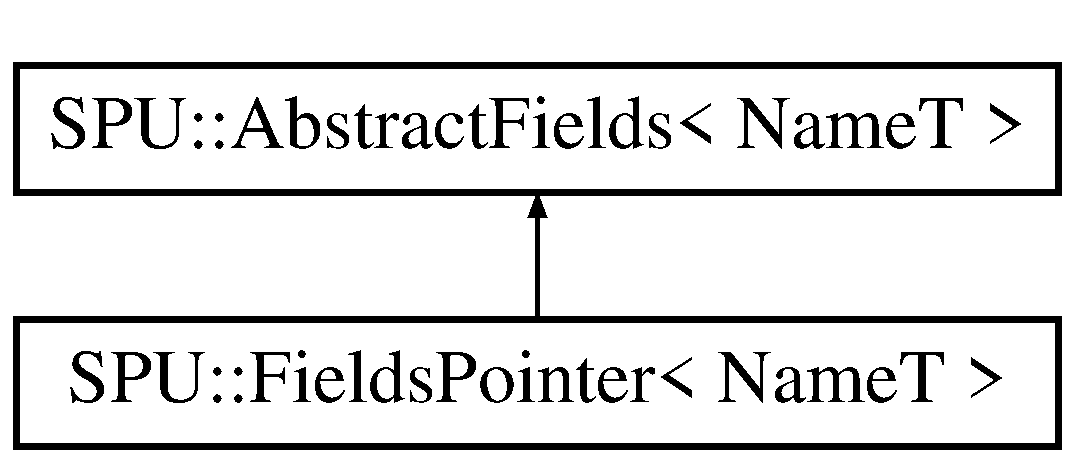
\includegraphics[height=2.000000cm]{class_s_p_u_1_1_fields_pointer}
\end{center}
\end{figure}
\doxysubsection*{Открытые члены}
\begin{DoxyCompactItemize}
\item 
\mbox{\Hypertarget{class_s_p_u_1_1_fields_pointer_a1a51ba42c450436c8822d3ec5e11d109}\label{class_s_p_u_1_1_fields_pointer_a1a51ba42c450436c8822d3ec5e11d109}} 
{\bfseries Fields\+Pointer} (\mbox{\hyperlink{class_s_p_u_1_1_fields}{Fields}}$<$ NameT $>$ $\ast$fields\+\_\+ptr)
\item 
\mbox{\Hypertarget{class_s_p_u_1_1_fields_pointer_a5aff44387a74225a711b00589573152a}\label{class_s_p_u_1_1_fields_pointer_a5aff44387a74225a711b00589573152a}} 
{\bfseries Fields\+Pointer} (const \mbox{\hyperlink{class_s_p_u_1_1_fields_pointer}{Fields\+Pointer}} \&other)
\item 
\mbox{\Hypertarget{class_s_p_u_1_1_fields_pointer_a3107ac0f1dda9f174ba1bfe7c1f7d638}\label{class_s_p_u_1_1_fields_pointer_a3107ac0f1dda9f174ba1bfe7c1f7d638}} 
{\bfseries operator data\+\_\+t} () override
\item 
\mbox{\Hypertarget{class_s_p_u_1_1_fields_pointer_aaf9e024f50093b5243a49899f03b26fc}\label{class_s_p_u_1_1_fields_pointer_aaf9e024f50093b5243a49899f03b26fc}} 
\mbox{\hyperlink{class_s_p_u_1_1_fields_pointer}{Fields\+Pointer}} \& {\bfseries operator=} (data\+\_\+t fields\+\_\+data) override
\item 
\mbox{\Hypertarget{class_s_p_u_1_1_fields_pointer_a7dd76bbfa5cfa8310c099eeb410b21ea}\label{class_s_p_u_1_1_fields_pointer_a7dd76bbfa5cfa8310c099eeb410b21ea}} 
\mbox{\hyperlink{class_s_p_u_1_1_fields_pointer}{Fields\+Pointer}} \& {\bfseries operator=} (\mbox{\hyperlink{class_s_p_u_1_1_fields_data}{Data}} fields\+\_\+data) override
\item 
\mbox{\Hypertarget{class_s_p_u_1_1_fields_pointer_a810d5b91571d4137bb81963915897b91}\label{class_s_p_u_1_1_fields_pointer_a810d5b91571d4137bb81963915897b91}} 
data\+\_\+t \& {\bfseries operator\mbox{[}$\,$\mbox{]}} (NameT name) override
\end{DoxyCompactItemize}
\doxysubsection*{Друзья}
\begin{DoxyCompactItemize}
\item 
\mbox{\Hypertarget{class_s_p_u_1_1_fields_pointer_aa8066818cce7efa3faa8e0117075ea63}\label{class_s_p_u_1_1_fields_pointer_aa8066818cce7efa3faa8e0117075ea63}} 
auto {\bfseries begin} (\mbox{\hyperlink{class_s_p_u_1_1_fields_pointer}{Fields\+Pointer}}$<$ NameT $>$ \&fields\+\_\+ptr)
\item 
\mbox{\Hypertarget{class_s_p_u_1_1_fields_pointer_aaa7f57577e0e7299836974c4f3c287ed}\label{class_s_p_u_1_1_fields_pointer_aaa7f57577e0e7299836974c4f3c287ed}} 
auto {\bfseries end} (\mbox{\hyperlink{class_s_p_u_1_1_fields_pointer}{Fields\+Pointer}}$<$ NameT $>$ \&fields\+\_\+ptr)
\end{DoxyCompactItemize}
\doxysubsection*{Дополнительные унаследованные члены}


Объявления и описания членов класса находятся в файле\+:\begin{DoxyCompactItemize}
\item 
spu-\/api/libspu/fields\+\_\+pointer.\+hpp\end{DoxyCompactItemize}

\hypertarget{class_s_p_u_1_1_fields_pointer_3_01void_01_4}{}\doxysection{Класс S\+PU\+::Fields\+Pointer$<$ void $>$}
\label{class_s_p_u_1_1_fields_pointer_3_01void_01_4}\index{SPU::FieldsPointer$<$ void $>$@{SPU::FieldsPointer$<$ void $>$}}
Граф наследования\+:S\+PU\+::Fields\+Pointer$<$ void $>$\+:\begin{figure}[H]
\begin{center}
\leavevmode
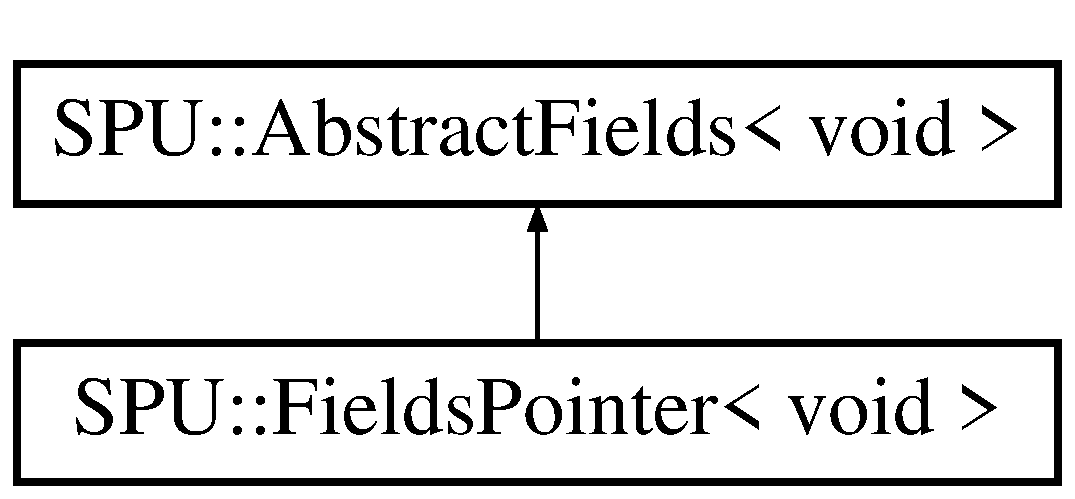
\includegraphics[height=2.000000cm]{class_s_p_u_1_1_fields_pointer_3_01void_01_4}
\end{center}
\end{figure}


Объявления и описания членов класса находятся в файле\+:\begin{DoxyCompactItemize}
\item 
spu-\/api/libspu/fields\+\_\+pointer.\+hpp\end{DoxyCompactItemize}

\hypertarget{class_s_p_u_1_1_fileops}{}\doxysection{Класс S\+PU\+::Fileops}
\label{class_s_p_u_1_1_fileops}\index{SPU::Fileops@{SPU::Fileops}}
\doxysubsection*{Открытые члены}
\begin{DoxyCompactItemize}
\item 
\mbox{\Hypertarget{class_s_p_u_1_1_fileops_a8db10c5df536ad53d91ce5bcfdaa706e}\label{class_s_p_u_1_1_fileops_a8db10c5df536ad53d91ce5bcfdaa706e}} 
{\bfseries Fileops} (const char $\ast$filename)
\item 
\mbox{\Hypertarget{class_s_p_u_1_1_fileops_a01121dc906965cc5ce3feba8dfbdcbec}\label{class_s_p_u_1_1_fileops_a01121dc906965cc5ce3feba8dfbdcbec}} 
{\footnotesize template$<$typename Cmd\+Frmt , typename Rslt\+Frmt $>$ }\\Rslt\+Frmt {\bfseries execute} (Cmd\+Frmt \&cmd)
\end{DoxyCompactItemize}


Объявления и описания членов класса находятся в файле\+:\begin{DoxyCompactItemize}
\item 
spu-\/api/libspu/fileops.\+hpp\end{DoxyCompactItemize}

\hypertarget{structfill__options}{}\section{Шаблон структуры fill\+\_\+options$<$ G $>$}
\label{structfill__options}\index{fill\+\_\+options$<$ G $>$@{fill\+\_\+options$<$ G $>$}}
\subsection*{Открытые типы}
\begin{DoxyCompactItemize}
\item 
\mbox{\Hypertarget{structfill__options_aa974f942fc0b1f8e3c92a347aadd8c01}\label{structfill__options_aa974f942fc0b1f8e3c92a347aadd8c01}} 
typedef graph\+\_\+traits$<$ G $>$\+::vertex\+\_\+descriptor {\bfseries vertex\+\_\+t}
\item 
\mbox{\Hypertarget{structfill__options_a763bee3dbe7df303af1f08cf6f497ce0}\label{structfill__options_a763bee3dbe7df303af1f08cf6f497ce0}} 
typedef graph\+\_\+traits$<$ G $>$\+::edge\+\_\+descriptor {\bfseries edge\+\_\+t}
\end{DoxyCompactItemize}
\subsection*{Открытые атрибуты}
\begin{DoxyCompactItemize}
\item 
\mbox{\Hypertarget{structfill__options_a2e6ed57c7f804b8d7208106b7874d1a2}\label{structfill__options_a2e6ed57c7f804b8d7208106b7874d1a2}} 
unsigned long {\bfseries rand\+\_\+init} = 0
\item 
\mbox{\Hypertarget{structfill__options_abeb37f9ba77fa19a79a59532e1b938c9}\label{structfill__options_abeb37f9ba77fa19a79a59532e1b938c9}} 
pair$<$ edge\+\_\+t, bool $>$($\ast$ {\bfseries add\+\_\+edge\+\_\+func} )(vertex\+\_\+t, vertex\+\_\+t, G \&) = nullptr
\end{DoxyCompactItemize}


Объявления и описания членов структуры находятся в файле\+:\begin{DoxyCompactItemize}
\item 
performance\+\_\+tests/utils.\+h\end{DoxyCompactItemize}

\hypertarget{struct_fixture}{}\section{Структура Fixture}
\label{struct_fixture}\index{Fixture@{Fixture}}
\subsection*{Открытые атрибуты}
\begin{DoxyCompactItemize}
\item 
\mbox{\Hypertarget{struct_fixture_a13638f842ef2a8714421ebe71ba98a39}\label{struct_fixture_a13638f842ef2a8714421ebe71ba98a39}} 
\hyperlink{class_s_p_u___g_r_a_p_h_1_1_spu_ultra_graph}{Spu\+Ultra\+Graph} {\bfseries graph}
\item 
\mbox{\Hypertarget{struct_fixture_a34b974dcb43215b8dfbc776ecccebc9c}\label{struct_fixture_a34b974dcb43215b8dfbc776ecccebc9c}} 
\hyperlink{structboost_1_1graph__test}{graph\+\_\+test}$<$ \hyperlink{class_s_p_u___g_r_a_p_h_1_1_spu_ultra_graph}{Spu\+Ultra\+Graph} $>$ {\bfseries graph\+\_\+tests}
\item 
\mbox{\Hypertarget{struct_fixture_a27efb5204a9c0630f2f5371ed3492943}\label{struct_fixture_a27efb5204a9c0630f2f5371ed3492943}} 
Spu\+Ultra\+Graph\+::vertex\+\_\+descriptor {\bfseries v1}
\item 
\mbox{\Hypertarget{struct_fixture_a574b245731c52555d692fa0c131489e2}\label{struct_fixture_a574b245731c52555d692fa0c131489e2}} 
Spu\+Ultra\+Graph\+::vertex\+\_\+descriptor {\bfseries v2}
\item 
\mbox{\Hypertarget{struct_fixture_a2f6bbeb63ad01ed7bf7daddd4c73a642}\label{struct_fixture_a2f6bbeb63ad01ed7bf7daddd4c73a642}} 
Spu\+Ultra\+Graph\+::vertex\+\_\+descriptor {\bfseries v3}
\item 
\mbox{\Hypertarget{struct_fixture_a14f9d6ac754e374afc2bd033b052f8ba}\label{struct_fixture_a14f9d6ac754e374afc2bd033b052f8ba}} 
Spu\+Ultra\+Graph\+::vertex\+\_\+descriptor {\bfseries v4}
\item 
\mbox{\Hypertarget{struct_fixture_af62f86e186965f464151593a98320f0d}\label{struct_fixture_af62f86e186965f464151593a98320f0d}} 
\hyperlink{class_s_p_u___g_r_a_p_h_1_1_spu_ultra_graph_a5f3776e003ef0a1648f1d9f84289810b}{Spu\+Ultra\+Graph\+::edge\+\_\+descriptor} {\bfseries e11}
\item 
\mbox{\Hypertarget{struct_fixture_a06aca3fe72ad21faab56f183ecbdd17c}\label{struct_fixture_a06aca3fe72ad21faab56f183ecbdd17c}} 
\hyperlink{class_s_p_u___g_r_a_p_h_1_1_spu_ultra_graph_a5f3776e003ef0a1648f1d9f84289810b}{Spu\+Ultra\+Graph\+::edge\+\_\+descriptor} {\bfseries e12\+\_\+1}
\item 
\mbox{\Hypertarget{struct_fixture_a26cbd640ca42b734a25d64033f19ef78}\label{struct_fixture_a26cbd640ca42b734a25d64033f19ef78}} 
\hyperlink{class_s_p_u___g_r_a_p_h_1_1_spu_ultra_graph_a5f3776e003ef0a1648f1d9f84289810b}{Spu\+Ultra\+Graph\+::edge\+\_\+descriptor} {\bfseries e12\+\_\+2}
\item 
\mbox{\Hypertarget{struct_fixture_a8add5ebbba1e293b961eb9fda0d141d0}\label{struct_fixture_a8add5ebbba1e293b961eb9fda0d141d0}} 
\hyperlink{class_s_p_u___g_r_a_p_h_1_1_spu_ultra_graph_a5f3776e003ef0a1648f1d9f84289810b}{Spu\+Ultra\+Graph\+::edge\+\_\+descriptor} {\bfseries e13}
\item 
\mbox{\Hypertarget{struct_fixture_a8bdd66984d5e0f2085c33f22ee25962f}\label{struct_fixture_a8bdd66984d5e0f2085c33f22ee25962f}} 
\hyperlink{class_s_p_u___g_r_a_p_h_1_1_spu_ultra_graph_a5f3776e003ef0a1648f1d9f84289810b}{Spu\+Ultra\+Graph\+::edge\+\_\+descriptor} {\bfseries e21}
\item 
\mbox{\Hypertarget{struct_fixture_a844fc9093ffa04a42186b22e1eebf4d9}\label{struct_fixture_a844fc9093ffa04a42186b22e1eebf4d9}} 
\hyperlink{class_s_p_u___g_r_a_p_h_1_1_spu_ultra_graph_a5f3776e003ef0a1648f1d9f84289810b}{Spu\+Ultra\+Graph\+::edge\+\_\+descriptor} {\bfseries e23}
\item 
\mbox{\Hypertarget{struct_fixture_af3989905bdf5788da2828f27eee8e653}\label{struct_fixture_af3989905bdf5788da2828f27eee8e653}} 
\hyperlink{class_s_p_u___g_r_a_p_h_1_1_spu_ultra_graph_a5f3776e003ef0a1648f1d9f84289810b}{Spu\+Ultra\+Graph\+::edge\+\_\+descriptor} {\bfseries e32}
\item 
\mbox{\Hypertarget{struct_fixture_a85d78773c6006be28ab68c513af0a047}\label{struct_fixture_a85d78773c6006be28ab68c513af0a047}} 
\hyperlink{class_s_p_u___g_r_a_p_h_1_1_spu_ultra_graph_a5f3776e003ef0a1648f1d9f84289810b}{Spu\+Ultra\+Graph\+::edge\+\_\+descriptor} {\bfseries e31}
\item 
\mbox{\Hypertarget{struct_fixture_a79c126342e64fca24e3307dce537528a}\label{struct_fixture_a79c126342e64fca24e3307dce537528a}} 
std\+::vector$<$ Spu\+Ultra\+Graph\+::vertex\+\_\+descriptor $>$ {\bfseries vertex\+\_\+set}
\item 
\mbox{\Hypertarget{struct_fixture_a543c399291942551c43dce0ffa4b7b6c}\label{struct_fixture_a543c399291942551c43dce0ffa4b7b6c}} 
std\+::vector$<$ std\+::pair$<$ Spu\+Ultra\+Graph\+::vertex\+\_\+descriptor, Spu\+Ultra\+Graph\+::vertex\+\_\+descriptor $>$ $>$ {\bfseries edge\+\_\+set}
\item 
\mbox{\Hypertarget{struct_fixture_abf9e07dce04da1900ca9b9652d0c4f18}\label{struct_fixture_abf9e07dce04da1900ca9b9652d0c4f18}} 
vector$<$ pair$<$ Spu\+Ultra\+Graph\+::vertex\+\_\+descriptor, value\+\_\+t $>$ $>$ {\bfseries vertex\+\_\+all\+\_\+props}
\item 
\mbox{\Hypertarget{struct_fixture_aa47a5a816608e13b46e9ceb1ee17a61a}\label{struct_fixture_aa47a5a816608e13b46e9ceb1ee17a61a}} 
\hyperlink{class_s_p_u_1_1_structure}{Structure} {\bfseries structure}
\item 
\mbox{\Hypertarget{struct_fixture_a333f197df82ad1755f5bda4b0d9aa431}\label{struct_fixture_a333f197df82ad1755f5bda4b0d9aa431}} 
\hyperlink{class_s_p_u___g_r_a_p_h_1_1_graph_structure}{Graph\+Structure} {\bfseries structure}
\end{DoxyCompactItemize}


Объявления и описания членов структур находятся в файлах\+:\begin{DoxyCompactItemize}
\item 
tests/test\+\_\+boost\+\_\+spu\+\_\+ultra\+\_\+graph.\+cpp\item 
tests/test\+\_\+spu\+\_\+api.\+cpp\item 
tests/test\+\_\+spu\+\_\+structure\+\_\+iterator.\+cpp\item 
tests/test\+\_\+spu\+\_\+ultra\+\_\+graph.\+cpp\end{DoxyCompactItemize}

\hypertarget{structboost_1_1graph__test}{}\section{Шаблон структуры boost\+:\+:graph\+\_\+test$<$ Graph $>$}
\label{structboost_1_1graph__test}\index{boost\+::graph\+\_\+test$<$ Graph $>$@{boost\+::graph\+\_\+test$<$ Graph $>$}}
\subsection*{Классы}
\begin{DoxyCompactItemize}
\item 
struct \hyperlink{structboost_1_1graph__test_1_1ignore__edge}{ignore\+\_\+edge}
\item 
struct \hyperlink{structboost_1_1graph__test_1_1ignore__edges}{ignore\+\_\+edges}
\item 
struct \hyperlink{structboost_1_1graph__test_1_1ignore__vertex}{ignore\+\_\+vertex}
\end{DoxyCompactItemize}
\subsection*{Открытые типы}
\begin{DoxyCompactItemize}
\item 
\mbox{\Hypertarget{structboost_1_1graph__test_ade600640dfb2ffd1bbcc4bb9db60a3f7}\label{structboost_1_1graph__test_ade600640dfb2ffd1bbcc4bb9db60a3f7}} 
typedef graph\+\_\+traits$<$ Graph $>$\+::vertex\+\_\+descriptor {\bfseries vertex\+\_\+t}
\item 
\mbox{\Hypertarget{structboost_1_1graph__test_af426fe5948619eec56e311e769173650}\label{structboost_1_1graph__test_af426fe5948619eec56e311e769173650}} 
typedef graph\+\_\+traits$<$ Graph $>$\+::edge\+\_\+descriptor {\bfseries edge\+\_\+t}
\item 
\mbox{\Hypertarget{structboost_1_1graph__test_a7cb70f96e2f1b68138299800859de7e8}\label{structboost_1_1graph__test_a7cb70f96e2f1b68138299800859de7e8}} 
typedef graph\+\_\+traits$<$ Graph $>$\+::vertices\+\_\+size\+\_\+type {\bfseries v\+\_\+size\+\_\+t}
\item 
\mbox{\Hypertarget{structboost_1_1graph__test_a063b71a61ac5e050f81bdb790bc88647}\label{structboost_1_1graph__test_a063b71a61ac5e050f81bdb790bc88647}} 
typedef graph\+\_\+traits$<$ Graph $>$\+::degree\+\_\+size\+\_\+type {\bfseries deg\+\_\+size\+\_\+t}
\item 
\mbox{\Hypertarget{structboost_1_1graph__test_a1c3818cea225fb663045266a1126a64e}\label{structboost_1_1graph__test_a1c3818cea225fb663045266a1126a64e}} 
typedef graph\+\_\+traits$<$ Graph $>$\+::edges\+\_\+size\+\_\+type {\bfseries e\+\_\+size\+\_\+t}
\item 
\mbox{\Hypertarget{structboost_1_1graph__test_ad37c27a29bf93c0df05d38b842e6cee1}\label{structboost_1_1graph__test_ad37c27a29bf93c0df05d38b842e6cee1}} 
typedef graph\+\_\+traits$<$ Graph $>$\+::out\+\_\+edge\+\_\+iterator {\bfseries out\+\_\+edge\+\_\+iter}
\item 
\mbox{\Hypertarget{structboost_1_1graph__test_abfc2081c0b9832f714e8da51f072c95f}\label{structboost_1_1graph__test_abfc2081c0b9832f714e8da51f072c95f}} 
typedef property\+\_\+map$<$ Graph, vertex\+\_\+index\+\_\+t $>$\+::type {\bfseries index\+\_\+map\+\_\+t}
\item 
\mbox{\Hypertarget{structboost_1_1graph__test_a5b4424db594ea6f0f239f40cff5d0034}\label{structboost_1_1graph__test_a5b4424db594ea6f0f239f40cff5d0034}} 
typedef iterator\+\_\+property\+\_\+map$<$ typename std\+::vector$<$ vertex\+\_\+t $>$\+::iterator, index\+\_\+map\+\_\+t, vertex\+\_\+t, vertex\+\_\+t \& $>$ {\bfseries Iso\+Map}
\end{DoxyCompactItemize}
\subsection*{Открытые члены}
\begin{DoxyCompactItemize}
\item 
\mbox{\Hypertarget{structboost_1_1graph__test_a1c7f7f3025d6523d3260544effcc8d35}\label{structboost_1_1graph__test_a1c7f7f3025d6523d3260544effcc8d35}} 
void {\bfseries test\+\_\+incidence\+\_\+graph} (const std\+::vector$<$ vertex\+\_\+t $>$ \&vertex\+\_\+set, const std\+::vector$<$ std\+::pair$<$ vertex\+\_\+t, vertex\+\_\+t $>$ $>$ \&edge\+\_\+set, const Graph \&g)
\item 
\mbox{\Hypertarget{structboost_1_1graph__test_aab436d06abc494be6a64da18ec09ecb3}\label{structboost_1_1graph__test_aab436d06abc494be6a64da18ec09ecb3}} 
void {\bfseries test\+\_\+bidirectional\+\_\+graph} (const std\+::vector$<$ vertex\+\_\+t $>$ \&vertex\+\_\+set, const std\+::vector$<$ std\+::pair$<$ vertex\+\_\+t, vertex\+\_\+t $>$ $>$ \&edge\+\_\+set, const Graph \&g)
\item 
\mbox{\Hypertarget{structboost_1_1graph__test_ab01e5d59de01d3a2f7a756142c3daef3}\label{structboost_1_1graph__test_ab01e5d59de01d3a2f7a756142c3daef3}} 
void {\bfseries test\+\_\+adjacency\+\_\+graph} (const std\+::vector$<$ vertex\+\_\+t $>$ \&vertex\+\_\+set, const std\+::vector$<$ std\+::pair$<$ vertex\+\_\+t, vertex\+\_\+t $>$ $>$ \&edge\+\_\+set, const Graph \&g)
\item 
\mbox{\Hypertarget{structboost_1_1graph__test_a6cf2bad7292277561a091d605022de3e}\label{structboost_1_1graph__test_a6cf2bad7292277561a091d605022de3e}} 
void {\bfseries test\+\_\+vertex\+\_\+list\+\_\+graph} (const std\+::vector$<$ vertex\+\_\+t $>$ \&vertex\+\_\+set, const Graph \&g)
\item 
\mbox{\Hypertarget{structboost_1_1graph__test_ada50db1e8060efeb6ed21843d46b5eb4}\label{structboost_1_1graph__test_ada50db1e8060efeb6ed21843d46b5eb4}} 
void {\bfseries test\+\_\+edge\+\_\+list\+\_\+graph} (const std\+::vector$<$ vertex\+\_\+t $>$ \&vertex\+\_\+set, const std\+::vector$<$ std\+::pair$<$ vertex\+\_\+t, vertex\+\_\+t $>$ $>$ \&edge\+\_\+set, const Graph \&g)
\item 
\mbox{\Hypertarget{structboost_1_1graph__test_a0cfbd7948aba361ecaf9242add8fd3b4}\label{structboost_1_1graph__test_a0cfbd7948aba361ecaf9242add8fd3b4}} 
void {\bfseries test\+\_\+adjacency\+\_\+matrix} (const std\+::vector$<$ vertex\+\_\+t $>$ \&vertex\+\_\+set, const std\+::vector$<$ std\+::pair$<$ vertex\+\_\+t, vertex\+\_\+t $>$ $>$ \&edge\+\_\+set, const Graph \&g)
\item 
\mbox{\Hypertarget{structboost_1_1graph__test_a353001b6205a774e1c01538b948cab21}\label{structboost_1_1graph__test_a353001b6205a774e1c01538b948cab21}} 
void {\bfseries test\+\_\+add\+\_\+vertex} (Graph \&g)
\item 
\mbox{\Hypertarget{structboost_1_1graph__test_ab1af5311dedf501d46ea89c702021410}\label{structboost_1_1graph__test_ab1af5311dedf501d46ea89c702021410}} 
void {\bfseries test\+\_\+add\+\_\+edge} (vertex\+\_\+t u, vertex\+\_\+t v, Graph \&g)
\item 
\mbox{\Hypertarget{structboost_1_1graph__test_ae769902ab95a2bd8a2665d30f97230c2}\label{structboost_1_1graph__test_ae769902ab95a2bd8a2665d30f97230c2}} 
void {\bfseries test\+\_\+remove\+\_\+edge} (vertex\+\_\+t u, vertex\+\_\+t v, Graph \&g)
\item 
\mbox{\Hypertarget{structboost_1_1graph__test_a52655c001000960e476e7eebcce0fa74}\label{structboost_1_1graph__test_a52655c001000960e476e7eebcce0fa74}} 
void {\bfseries test\+\_\+remove\+\_\+edge} (edge\+\_\+t e, Graph \&g)
\item 
\mbox{\Hypertarget{structboost_1_1graph__test_aabd61820629d6c8355c840f37a006250}\label{structboost_1_1graph__test_aabd61820629d6c8355c840f37a006250}} 
void {\bfseries test\+\_\+clear\+\_\+vertex} (vertex\+\_\+t v, Graph \&g)
\item 
\mbox{\Hypertarget{structboost_1_1graph__test_a799ea10186b6a78ee02b2d0ef903f0fd}\label{structboost_1_1graph__test_a799ea10186b6a78ee02b2d0ef903f0fd}} 
{\footnotesize template$<$typename Prop\+Val , typename Property\+Tag $>$ }\\void {\bfseries test\+\_\+readable\+\_\+vertex\+\_\+property\+\_\+graph} (const std\+::vector$<$ Prop\+Val $>$ \&vertex\+\_\+prop, Property\+Tag tag, const Graph \&g)
\item 
\mbox{\Hypertarget{structboost_1_1graph__test_a77e36a1f163c6c8c73a62954503bb21c}\label{structboost_1_1graph__test_a77e36a1f163c6c8c73a62954503bb21c}} 
{\footnotesize template$<$typename Prop\+Val , typename Property\+Tag $>$ }\\void {\bfseries test\+\_\+vertex\+\_\+property\+\_\+graph} (const std\+::vector$<$ Prop\+Val $>$ \&vertex\+\_\+prop, Property\+Tag tag, Graph \&g)
\end{DoxyCompactItemize}


Объявления и описания членов структуры находятся в файле\+:\begin{DoxyCompactItemize}
\item 
tests/graph\+\_\+test.\+h\end{DoxyCompactItemize}

\hypertarget{class_graph_performance_test}{}\section{Шаблон класса Graph\+Performance\+Test$<$ G $>$}
\label{class_graph_performance_test}\index{Graph\+Performance\+Test$<$ G $>$@{Graph\+Performance\+Test$<$ G $>$}}
\subsection*{Открытые члены}
\begin{DoxyCompactItemize}
\item 
\mbox{\Hypertarget{class_graph_performance_test_a51b3b8479660b36be84e608549391244}\label{class_graph_performance_test_a51b3b8479660b36be84e608549391244}} 
{\bfseries Graph\+Performance\+Test} (void($\ast$test\+\_\+func)(G \&), string results\+\_\+file)
\item 
\mbox{\Hypertarget{class_graph_performance_test_a4b8bbf9ae4678e78d4c9a0dc938df598}\label{class_graph_performance_test_a4b8bbf9ae4678e78d4c9a0dc938df598}} 
void {\bfseries start} ()
\end{DoxyCompactItemize}
\subsection*{Открытые атрибуты}
\begin{DoxyCompactItemize}
\item 
\mbox{\Hypertarget{class_graph_performance_test_a6a81e81b07a591860d0a1183ed05f023}\label{class_graph_performance_test_a6a81e81b07a591860d0a1183ed05f023}} 
void($\ast$ {\bfseries test\+\_\+func} )(G \&) = nullptr
\item 
\mbox{\Hypertarget{class_graph_performance_test_a29b8d1216b085d2e59b9373e57e8c215}\label{class_graph_performance_test_a29b8d1216b085d2e59b9373e57e8c215}} 
string {\bfseries results\+\_\+file} = \char`\"{}results.\+csv\char`\"{}
\item 
\mbox{\Hypertarget{class_graph_performance_test_aea61a34b1ef7ae8c1c33361242c2c7c4}\label{class_graph_performance_test_aea61a34b1ef7ae8c1c33361242c2c7c4}} 
size\+\_\+t {\bfseries avg\+\_\+iterations\+\_\+cnt} = 3
\item 
\mbox{\Hypertarget{class_graph_performance_test_a76c584ed92d5cb9bfe5c7f454fb3d437}\label{class_graph_performance_test_a76c584ed92d5cb9bfe5c7f454fb3d437}} 
bool {\bfseries should\+\_\+fill} = true
\item 
\mbox{\Hypertarget{class_graph_performance_test_a827065a47360940a0f32c190ad66988b}\label{class_graph_performance_test_a827065a47360940a0f32c190ad66988b}} 
bool {\bfseries is\+\_\+mutable\+\_\+test} = true
\item 
\mbox{\Hypertarget{class_graph_performance_test_a3a6c213cd32e751e1652c97397340bd7}\label{class_graph_performance_test_a3a6c213cd32e751e1652c97397340bd7}} 
pair$<$ edge\+\_\+t, bool $>$($\ast$ {\bfseries add\+\_\+edge\+\_\+func} )(vertex\+\_\+t, vertex\+\_\+t, G \&) = nullptr
\item 
\mbox{\Hypertarget{class_graph_performance_test_ad2d7566c76d0743fd89a6e74f5280100}\label{class_graph_performance_test_ad2d7566c76d0743fd89a6e74f5280100}} 
size\+\_\+t {\bfseries start\+\_\+vertices\+\_\+cnt} = 1000
\item 
\mbox{\Hypertarget{class_graph_performance_test_a5335c67d0198d70412f02a0a14a38fa2}\label{class_graph_performance_test_a5335c67d0198d70412f02a0a14a38fa2}} 
size\+\_\+t {\bfseries inc\+\_\+vertices\+\_\+value} = 1000
\item 
\mbox{\Hypertarget{class_graph_performance_test_a68c14062ddb3bfcbd7a9957fc3d211a2}\label{class_graph_performance_test_a68c14062ddb3bfcbd7a9957fc3d211a2}} 
size\+\_\+t {\bfseries end\+\_\+vertices\+\_\+cnt} = 100000
\item 
\mbox{\Hypertarget{class_graph_performance_test_af1ffbabe05d708b11769fdc3d0004dba}\label{class_graph_performance_test_af1ffbabe05d708b11769fdc3d0004dba}} 
size\+\_\+t {\bfseries edges\+\_\+per\+\_\+vertex} = 2
\end{DoxyCompactItemize}


Объявления и описания членов класса находятся в файле\+:\begin{DoxyCompactItemize}
\item 
performance\+\_\+tests/Graph\+Performance\+Test.\+h\end{DoxyCompactItemize}

\hypertarget{class_s_p_u___g_r_a_p_h_1_1_graph_structure}{}\doxysection{Класс S\+P\+U\+\_\+\+G\+R\+A\+PH\+::Graph\+Structure}
\label{class_s_p_u___g_r_a_p_h_1_1_graph_structure}\index{SPU\_GRAPH::GraphStructure@{SPU\_GRAPH::GraphStructure}}
\doxysubsection*{Открытые члены}
\begin{DoxyCompactItemize}
\item 
\mbox{\Hypertarget{class_s_p_u___g_r_a_p_h_1_1_graph_structure_ae1e2535a2ac2bfecb0bfbf68f4635d75}\label{class_s_p_u___g_r_a_p_h_1_1_graph_structure_ae1e2535a2ac2bfecb0bfbf68f4635d75}} 
{\bfseries Graph\+Structure} (std\+::shared\+\_\+ptr$<$ \mbox{\hyperlink{class_s_p_u_1_1_abstract_structure}{Abstract\+Structure}} $>$ structure)
\item 
\mbox{\Hypertarget{class_s_p_u___g_r_a_p_h_1_1_graph_structure_a7a5ad16ffbf2d3d50e5a0453d5c9b225}\label{class_s_p_u___g_r_a_p_h_1_1_graph_structure_a7a5ad16ffbf2d3d50e5a0453d5c9b225}} 
void {\bfseries set} (std\+::shared\+\_\+ptr$<$ \mbox{\hyperlink{class_s_p_u_1_1_structure}{Structure}}$<$$>$$>$ structure)
\item 
\mbox{\Hypertarget{class_s_p_u___g_r_a_p_h_1_1_graph_structure_a6f2f2bfb7a31de1d5eaa6e10c70b1fc1}\label{class_s_p_u___g_r_a_p_h_1_1_graph_structure_a6f2f2bfb7a31de1d5eaa6e10c70b1fc1}} 
\mbox{\hyperlink{class_s_p_u___g_r_a_p_h_1_1_graph_structure}{Graph\+Structure}} \& {\bfseries operator=} (std\+::shared\+\_\+ptr$<$ \mbox{\hyperlink{class_s_p_u_1_1_abstract_structure}{Abstract\+Structure}} $>$ structure)
\item 
\mbox{\Hypertarget{class_s_p_u___g_r_a_p_h_1_1_graph_structure_ae1562708dc137727326734aa3ce6827e}\label{class_s_p_u___g_r_a_p_h_1_1_graph_structure_ae1562708dc137727326734aa3ce6827e}} 
status\+\_\+t {\bfseries insert} (S\+P\+U\+::key\+\_\+t key, value\+\_\+t value=\{0\}, flags\+\_\+t flags=N\+O\+\_\+\+F\+L\+A\+GS)
\item 
\mbox{\Hypertarget{class_s_p_u___g_r_a_p_h_1_1_graph_structure_a46058b12a8024e7d9c32e995350c61d9}\label{class_s_p_u___g_r_a_p_h_1_1_graph_structure_a46058b12a8024e7d9c32e995350c61d9}} 
status\+\_\+t {\bfseries del} (S\+P\+U\+::key\+\_\+t key, flags\+\_\+t flags=N\+O\+\_\+\+F\+L\+A\+GS)
\item 
\mbox{\Hypertarget{class_s_p_u___g_r_a_p_h_1_1_graph_structure_a2b25832c46aee724f5a91b32cbe5971b}\label{class_s_p_u___g_r_a_p_h_1_1_graph_structure_a2b25832c46aee724f5a91b32cbe5971b}} 
\mbox{\hyperlink{struct_s_p_u_1_1pair__containter}{pair\+\_\+t}} {\bfseries search} (S\+P\+U\+::key\+\_\+t key, flags\+\_\+t flags=P\+\_\+\+F\+L\+AG) const
\item 
\mbox{\Hypertarget{class_s_p_u___g_r_a_p_h_1_1_graph_structure_ab9adcc555bb778d96d5e70cefdf48198}\label{class_s_p_u___g_r_a_p_h_1_1_graph_structure_ab9adcc555bb778d96d5e70cefdf48198}} 
\mbox{\hyperlink{struct_s_p_u_1_1pair__containter}{pair\+\_\+t}} {\bfseries min} (flags\+\_\+t flags=P\+\_\+\+F\+L\+AG) const
\item 
\mbox{\Hypertarget{class_s_p_u___g_r_a_p_h_1_1_graph_structure_acfd4c9bb9d07d1e5daf4de3d159fad10}\label{class_s_p_u___g_r_a_p_h_1_1_graph_structure_acfd4c9bb9d07d1e5daf4de3d159fad10}} 
\mbox{\hyperlink{struct_s_p_u_1_1pair__containter}{pair\+\_\+t}} {\bfseries max} (flags\+\_\+t flags=P\+\_\+\+F\+L\+AG) const
\item 
\mbox{\Hypertarget{class_s_p_u___g_r_a_p_h_1_1_graph_structure_a089e2778b479b47b709bafdb16f71e7b}\label{class_s_p_u___g_r_a_p_h_1_1_graph_structure_a089e2778b479b47b709bafdb16f71e7b}} 
\mbox{\hyperlink{struct_s_p_u_1_1pair__containter}{pair\+\_\+t}} {\bfseries next} (S\+P\+U\+::key\+\_\+t key, flags\+\_\+t flags=P\+\_\+\+F\+L\+AG) const
\item 
\mbox{\Hypertarget{class_s_p_u___g_r_a_p_h_1_1_graph_structure_ac3d52277ac2153404de9b9c6e6e6cef6}\label{class_s_p_u___g_r_a_p_h_1_1_graph_structure_ac3d52277ac2153404de9b9c6e6e6cef6}} 
\mbox{\hyperlink{struct_s_p_u_1_1pair__containter}{pair\+\_\+t}} {\bfseries prev} (S\+P\+U\+::key\+\_\+t key, flags\+\_\+t flags=P\+\_\+\+F\+L\+AG) const
\item 
\mbox{\Hypertarget{class_s_p_u___g_r_a_p_h_1_1_graph_structure_a4132720a0585b471da3d7e67628f0360}\label{class_s_p_u___g_r_a_p_h_1_1_graph_structure_a4132720a0585b471da3d7e67628f0360}} 
\mbox{\hyperlink{struct_s_p_u_1_1pair__containter}{pair\+\_\+t}} {\bfseries nsm} (S\+P\+U\+::key\+\_\+t key, flags\+\_\+t flags=P\+\_\+\+F\+L\+AG) const
\item 
\mbox{\Hypertarget{class_s_p_u___g_r_a_p_h_1_1_graph_structure_a2dc44fa2e81cf9740b34c81a11f3b854}\label{class_s_p_u___g_r_a_p_h_1_1_graph_structure_a2dc44fa2e81cf9740b34c81a11f3b854}} 
\mbox{\hyperlink{struct_s_p_u_1_1pair__containter}{pair\+\_\+t}} {\bfseries ngr} (S\+P\+U\+::key\+\_\+t key, flags\+\_\+t flags=P\+\_\+\+F\+L\+AG) const
\end{DoxyCompactItemize}


Объявления и описания членов класса находятся в файле\+:\begin{DoxyCompactItemize}
\item 
Graph\+Structure.\+h\end{DoxyCompactItemize}

\hypertarget{structgsid__container}{}\doxysection{Структура gsid\+\_\+container}
\label{structgsid__container}\index{gsid\_container@{gsid\_container}}
\doxysubsection*{Открытые атрибуты}
\begin{DoxyCompactItemize}
\item 
\mbox{\Hypertarget{structgsid__container_a59c431b036194c920a77dce89e025109}\label{structgsid__container_a59c431b036194c920a77dce89e025109}} 
u32 {\bfseries cont} \mbox{[}G\+S\+I\+D\+\_\+\+W\+E\+I\+G\+HT\mbox{]}
\end{DoxyCompactItemize}


Объявления и описания членов структуры находятся в файле\+:\begin{DoxyCompactItemize}
\item 
spu-\/api/libspu/spu.\+h\end{DoxyCompactItemize}

\hypertarget{class_s_p_u_1_1_hash_map_extern_value}{}\section{Шаблон класса S\+PU\+:\+:Hash\+Map\+Extern\+Value$<$ T $>$}
\label{class_s_p_u_1_1_hash_map_extern_value}\index{S\+P\+U\+::\+Hash\+Map\+Extern\+Value$<$ T $>$@{S\+P\+U\+::\+Hash\+Map\+Extern\+Value$<$ T $>$}}
Граф наследования\+:S\+PU\+:\+:Hash\+Map\+Extern\+Value$<$ T $>$\+:\begin{figure}[H]
\begin{center}
\leavevmode
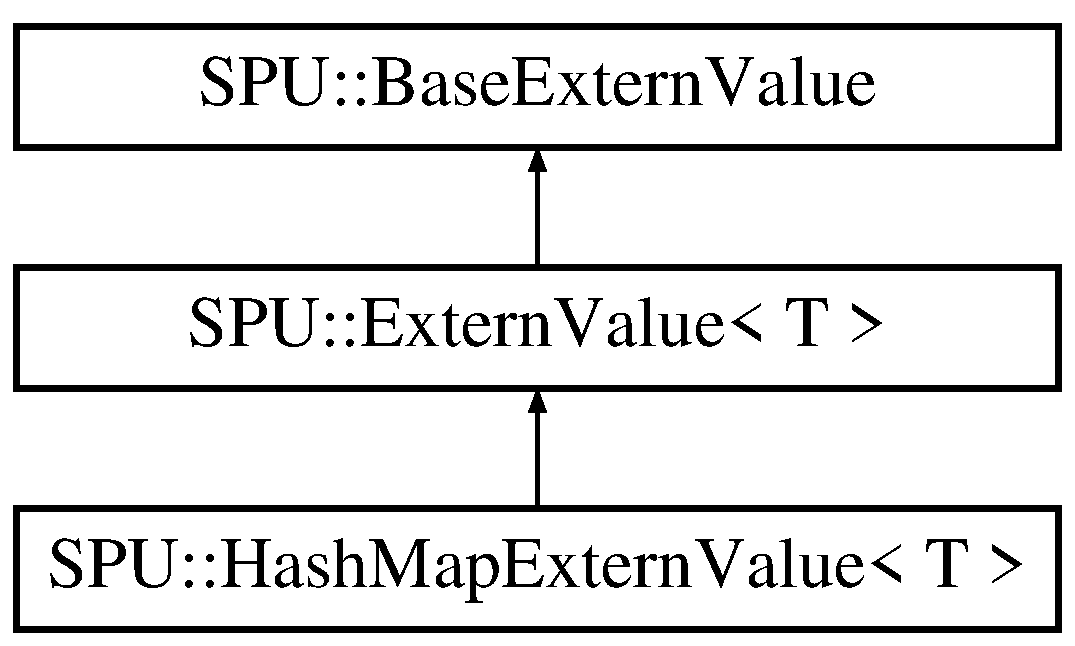
\includegraphics[height=3.000000cm]{class_s_p_u_1_1_hash_map_extern_value}
\end{center}
\end{figure}
\subsection*{Открытые члены}
\begin{DoxyCompactItemize}
\item 
\mbox{\Hypertarget{class_s_p_u_1_1_hash_map_extern_value_aedfc6561bfed0ccddd500a92d7edeb57}\label{class_s_p_u_1_1_hash_map_extern_value_aedfc6561bfed0ccddd500a92d7edeb57}} 
{\bfseries Hash\+Map\+Extern\+Value} (value\+\_\+t id)
\item 
\mbox{\Hypertarget{class_s_p_u_1_1_hash_map_extern_value_aeb39b3476529c443c306237063ea6d60}\label{class_s_p_u_1_1_hash_map_extern_value_aeb39b3476529c443c306237063ea6d60}} 
{\bfseries Hash\+Map\+Extern\+Value} (\hyperlink{struct_s_p_u_1_1pair__containter}{pair\+\_\+t} pair)
\item 
\mbox{\Hypertarget{class_s_p_u_1_1_hash_map_extern_value_a2d55cbd44a157910b09f3ef38836c4ae}\label{class_s_p_u_1_1_hash_map_extern_value_a2d55cbd44a157910b09f3ef38836c4ae}} 
{\bfseries Hash\+Map\+Extern\+Value} (T value)
\item 
\mbox{\Hypertarget{class_s_p_u_1_1_hash_map_extern_value_a0d88f76795e84dee2c8c65fb3f4583cc}\label{class_s_p_u_1_1_hash_map_extern_value_a0d88f76795e84dee2c8c65fb3f4583cc}} 
T \& {\bfseries get} () override
\item 
\mbox{\Hypertarget{class_s_p_u_1_1_hash_map_extern_value_af8b1efec472cfe183151aa7301941dc5}\label{class_s_p_u_1_1_hash_map_extern_value_af8b1efec472cfe183151aa7301941dc5}} 
void {\bfseries set} (T value) override
\end{DoxyCompactItemize}
\subsection*{Дополнительные унаследованные члены}


Объявления и описания членов класса находятся в файле\+:\begin{DoxyCompactItemize}
\item 
spu-\/api/libspu/extern\+\_\+value.\+hpp\end{DoxyCompactItemize}

\hypertarget{structboost_1_1graph__test_1_1ignore__edge}{}\doxysection{Структура boost\+::graph\+\_\+test$<$ Graph $>$\+::ignore\+\_\+edge}
\label{structboost_1_1graph__test_1_1ignore__edge}\index{boost::graph\_test$<$ Graph $>$::ignore\_edge@{boost::graph\_test$<$ Graph $>$::ignore\_edge}}
\doxysubsection*{Открытые члены}
\begin{DoxyCompactItemize}
\item 
\mbox{\Hypertarget{structboost_1_1graph__test_1_1ignore__edge_a83cdc37986d330481abd87d49195dd25}\label{structboost_1_1graph__test_1_1ignore__edge_a83cdc37986d330481abd87d49195dd25}} 
{\bfseries ignore\+\_\+edge} (edge\+\_\+t e)
\item 
\mbox{\Hypertarget{structboost_1_1graph__test_1_1ignore__edge_a3515fdaf8d0f89bc9c00182443c41e97}\label{structboost_1_1graph__test_1_1ignore__edge_a3515fdaf8d0f89bc9c00182443c41e97}} 
bool {\bfseries operator()} (edge\+\_\+t x) const
\end{DoxyCompactItemize}
\doxysubsection*{Открытые атрибуты}
\begin{DoxyCompactItemize}
\item 
\mbox{\Hypertarget{structboost_1_1graph__test_1_1ignore__edge_ad51c6031e8dea8f7e0d9ae02ce752885}\label{structboost_1_1graph__test_1_1ignore__edge_ad51c6031e8dea8f7e0d9ae02ce752885}} 
edge\+\_\+t {\bfseries e}
\end{DoxyCompactItemize}


Объявления и описания членов структуры находятся в файле\+:\begin{DoxyCompactItemize}
\item 
tests/graph\+\_\+test.\+h\end{DoxyCompactItemize}

\hypertarget{structboost_1_1graph__test_1_1ignore__edges}{}\section{Структура boost\+:\+:graph\+\_\+test$<$ Graph $>$\+:\+:ignore\+\_\+edges}
\label{structboost_1_1graph__test_1_1ignore__edges}\index{boost\+::graph\+\_\+test$<$ Graph $>$\+::ignore\+\_\+edges@{boost\+::graph\+\_\+test$<$ Graph $>$\+::ignore\+\_\+edges}}
\subsection*{Открытые члены}
\begin{DoxyCompactItemize}
\item 
\mbox{\Hypertarget{structboost_1_1graph__test_1_1ignore__edges_ab61f187b8da8f7a48b2422632e600d32}\label{structboost_1_1graph__test_1_1ignore__edges_ab61f187b8da8f7a48b2422632e600d32}} 
{\bfseries ignore\+\_\+edges} (vertex\+\_\+t s, vertex\+\_\+t t, const Graph \&g)
\item 
\mbox{\Hypertarget{structboost_1_1graph__test_1_1ignore__edges_a81277c81f4356e085bde27496e447dce}\label{structboost_1_1graph__test_1_1ignore__edges_a81277c81f4356e085bde27496e447dce}} 
bool {\bfseries operator()} (edge\+\_\+t x) const
\end{DoxyCompactItemize}
\subsection*{Открытые атрибуты}
\begin{DoxyCompactItemize}
\item 
\mbox{\Hypertarget{structboost_1_1graph__test_1_1ignore__edges_a1ba173edcdc2115a8fb8d8711ea37064}\label{structboost_1_1graph__test_1_1ignore__edges_a1ba173edcdc2115a8fb8d8711ea37064}} 
vertex\+\_\+t {\bfseries s}
\item 
\mbox{\Hypertarget{structboost_1_1graph__test_1_1ignore__edges_a1567af3a3a271fe2b85001c25cb092fb}\label{structboost_1_1graph__test_1_1ignore__edges_a1567af3a3a271fe2b85001c25cb092fb}} 
vertex\+\_\+t {\bfseries t}
\item 
\mbox{\Hypertarget{structboost_1_1graph__test_1_1ignore__edges_a154cb99d11abcbd0f1195b75eeb8c44c}\label{structboost_1_1graph__test_1_1ignore__edges_a154cb99d11abcbd0f1195b75eeb8c44c}} 
Graph $\ast$ {\bfseries g}
\end{DoxyCompactItemize}


Объявления и описания членов структуры находятся в файле\+:\begin{DoxyCompactItemize}
\item 
tests/graph\+\_\+test.\+h\end{DoxyCompactItemize}

\hypertarget{structboost_1_1graph__test_1_1ignore__vertex}{}\section{Структура boost\+:\+:graph\+\_\+test$<$ Graph $>$\+:\+:ignore\+\_\+vertex}
\label{structboost_1_1graph__test_1_1ignore__vertex}\index{boost\+::graph\+\_\+test$<$ Graph $>$\+::ignore\+\_\+vertex@{boost\+::graph\+\_\+test$<$ Graph $>$\+::ignore\+\_\+vertex}}
\subsection*{Открытые члены}
\begin{DoxyCompactItemize}
\item 
\mbox{\Hypertarget{structboost_1_1graph__test_1_1ignore__vertex_a3b0a8c0b55d383b7aed8f155097180ff}\label{structboost_1_1graph__test_1_1ignore__vertex_a3b0a8c0b55d383b7aed8f155097180ff}} 
{\bfseries ignore\+\_\+vertex} (vertex\+\_\+t v)
\item 
\mbox{\Hypertarget{structboost_1_1graph__test_1_1ignore__vertex_aa4fe8b58fd0e483b16afa523ddaf9322}\label{structboost_1_1graph__test_1_1ignore__vertex_aa4fe8b58fd0e483b16afa523ddaf9322}} 
bool {\bfseries operator()} (vertex\+\_\+t x) const
\end{DoxyCompactItemize}
\subsection*{Открытые атрибуты}
\begin{DoxyCompactItemize}
\item 
\mbox{\Hypertarget{structboost_1_1graph__test_1_1ignore__vertex_adcaccee3f1f378199eca3b00886cc3f2}\label{structboost_1_1graph__test_1_1ignore__vertex_adcaccee3f1f378199eca3b00886cc3f2}} 
vertex\+\_\+t {\bfseries v}
\end{DoxyCompactItemize}


Объявления и описания членов структуры находятся в файле\+:\begin{DoxyCompactItemize}
\item 
tests/graph\+\_\+test.\+h\end{DoxyCompactItemize}

\hypertarget{struct_s_p_u_1_1_abstract_structure_1_1_insert_struct}{}\section{Структура S\+PU\+:\+:Abstract\+Structure\+:\+:Insert\+Struct}
\label{struct_s_p_u_1_1_abstract_structure_1_1_insert_struct}\index{S\+P\+U\+::\+Abstract\+Structure\+::\+Insert\+Struct@{S\+P\+U\+::\+Abstract\+Structure\+::\+Insert\+Struct}}
\subsection*{Открытые атрибуты}
\begin{DoxyCompactItemize}
\item 
\mbox{\Hypertarget{struct_s_p_u_1_1_abstract_structure_1_1_insert_struct_abf1aea5844ee2b375fced121ad49187d}\label{struct_s_p_u_1_1_abstract_structure_1_1_insert_struct_abf1aea5844ee2b375fced121ad49187d}} 
key\+\_\+t {\bfseries key}
\item 
\mbox{\Hypertarget{struct_s_p_u_1_1_abstract_structure_1_1_insert_struct_a40b28c3114c043363f3c3dc024d016cf}\label{struct_s_p_u_1_1_abstract_structure_1_1_insert_struct_a40b28c3114c043363f3c3dc024d016cf}} 
value\+\_\+t {\bfseries value}
\end{DoxyCompactItemize}


Объявления и описания членов структуры находятся в файле\+:\begin{DoxyCompactItemize}
\item 
spu-\/api/libspu/abstract\+\_\+structure.\+hpp\end{DoxyCompactItemize}

\hypertarget{class_insufficient_storage}{}\doxysection{Класс Insufficient\+Storage}
\label{class_insufficient_storage}\index{InsufficientStorage@{InsufficientStorage}}
Граф наследования\+:Insufficient\+Storage\+:\begin{figure}[H]
\begin{center}
\leavevmode
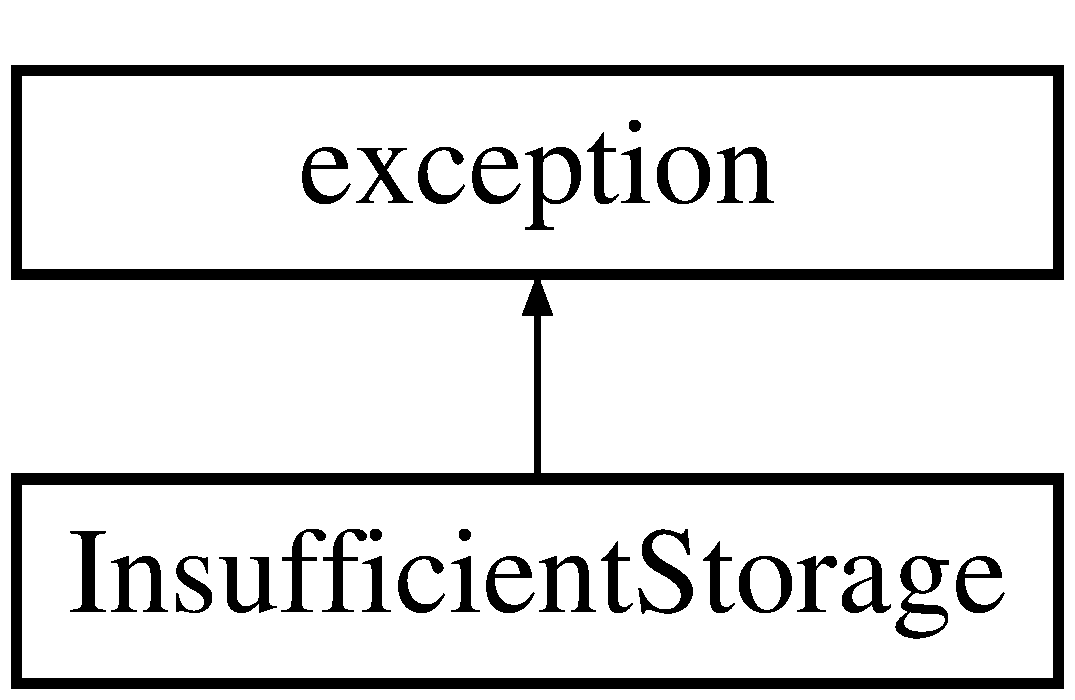
\includegraphics[height=2.000000cm]{class_insufficient_storage}
\end{center}
\end{figure}
\doxysubsection*{Открытые члены}
\begin{DoxyCompactItemize}
\item 
\mbox{\Hypertarget{class_insufficient_storage_a59e341b5e13ba88092f7faf478268fd4}\label{class_insufficient_storage_a59e341b5e13ba88092f7faf478268fd4}} 
{\bfseries Insufficient\+Storage} (const string \&error=\char`\"{}Insufficient Storage\char`\"{})
\item 
\mbox{\Hypertarget{class_insufficient_storage_aa2807f5c9094788feb47434e735e9af0}\label{class_insufficient_storage_aa2807f5c9094788feb47434e735e9af0}} 
const char $\ast$ {\bfseries what} () const noexcept override
\end{DoxyCompactItemize}


Объявления и описания членов класса находятся в файле\+:\begin{DoxyCompactItemize}
\item 
exceptions.\+h\end{DoxyCompactItemize}

\hypertarget{struct_s_p_u_1_1_no_fields_data}{}\section{Структура S\+PU\+:\+:No\+Fields\+Data}
\label{struct_s_p_u_1_1_no_fields_data}\index{S\+P\+U\+::\+No\+Fields\+Data@{S\+P\+U\+::\+No\+Fields\+Data}}
Граф наследования\+:S\+PU\+:\+:No\+Fields\+Data\+:\begin{figure}[H]
\begin{center}
\leavevmode
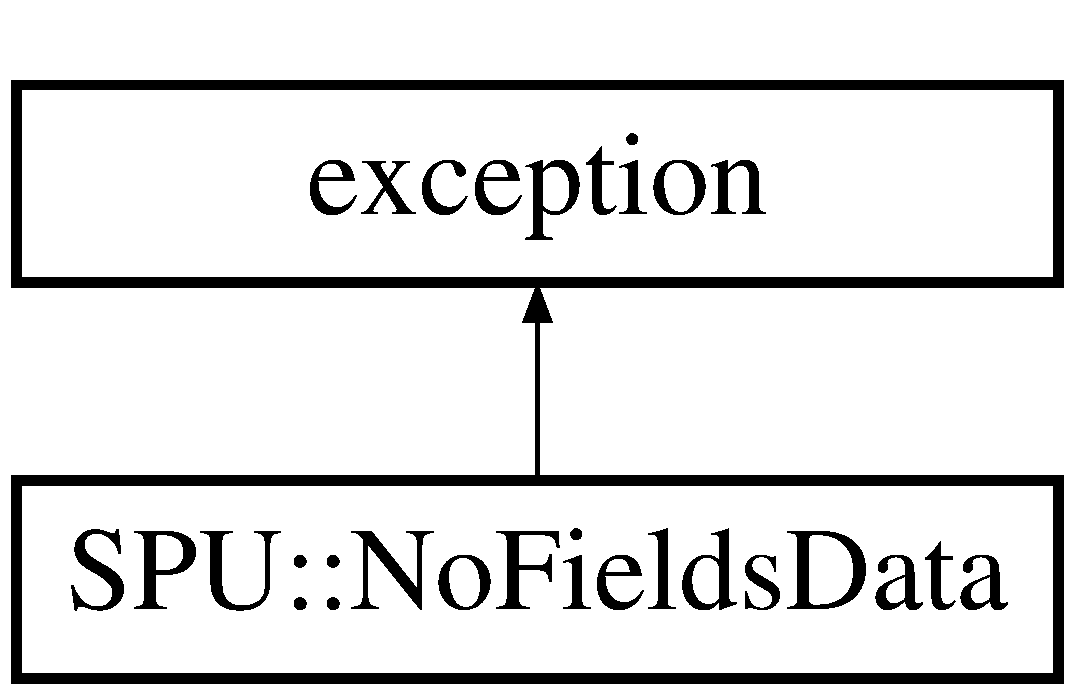
\includegraphics[height=2.000000cm]{struct_s_p_u_1_1_no_fields_data}
\end{center}
\end{figure}
\subsection*{Открытые члены}
\begin{DoxyCompactItemize}
\item 
\mbox{\Hypertarget{struct_s_p_u_1_1_no_fields_data_a7eee5209ec03f5ba6f69efbf247a25e0}\label{struct_s_p_u_1_1_no_fields_data_a7eee5209ec03f5ba6f69efbf247a25e0}} 
const char $\ast$ {\bfseries what} () const  throw ()
\end{DoxyCompactItemize}


Объявления и описания членов структуры находятся в файле\+:\begin{DoxyCompactItemize}
\item 
spu-\/api/libspu/errors/no\+\_\+fields\+\_\+data.\+hpp\end{DoxyCompactItemize}

\hypertarget{class_not_found}{}\section{Класс Not\+Found}
\label{class_not_found}\index{Not\+Found@{Not\+Found}}
Граф наследования\+:Not\+Found\+:\begin{figure}[H]
\begin{center}
\leavevmode
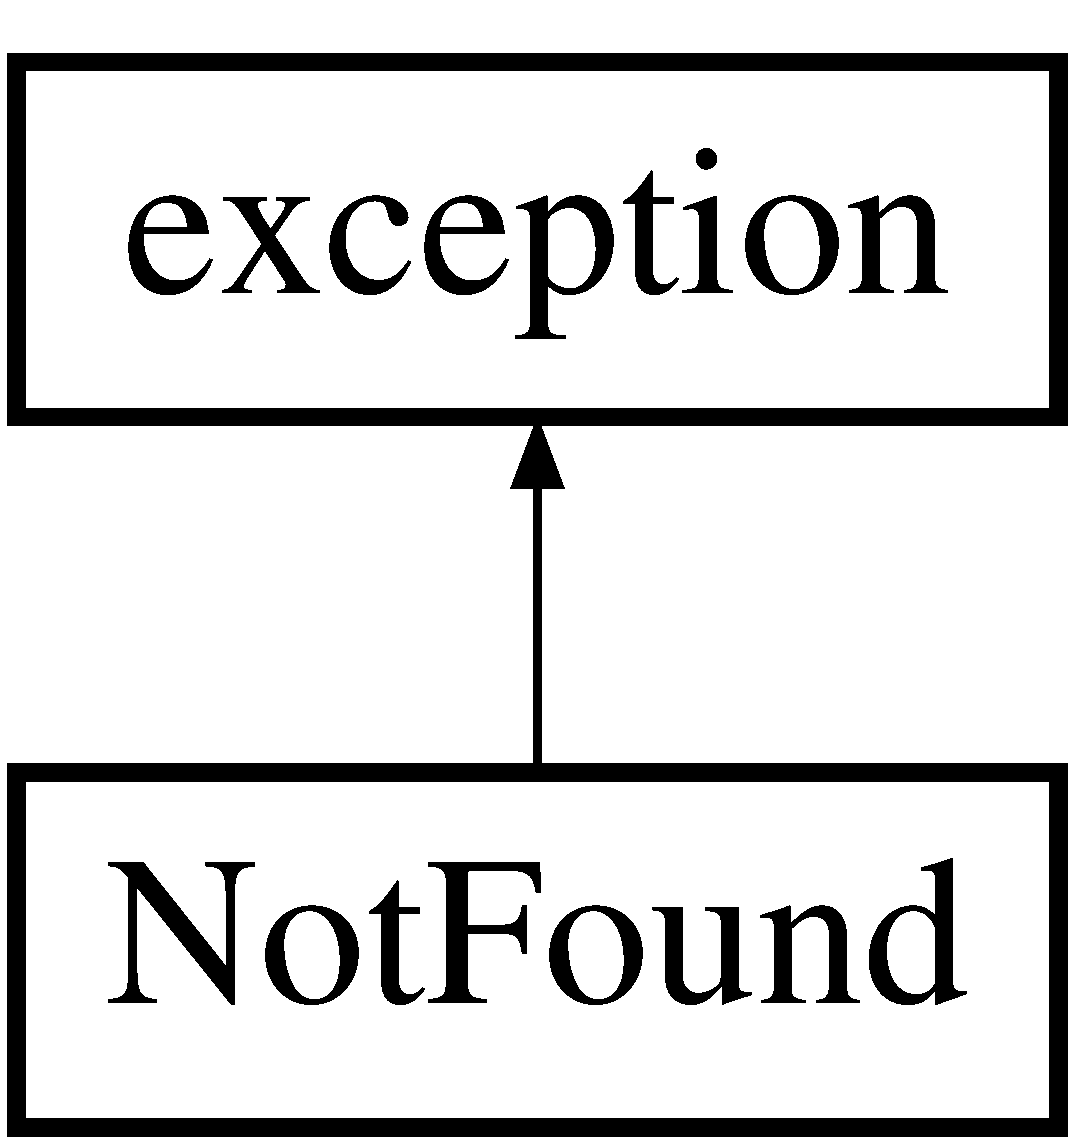
\includegraphics[height=2.000000cm]{class_not_found}
\end{center}
\end{figure}
\subsection*{Открытые члены}
\begin{DoxyCompactItemize}
\item 
\mbox{\Hypertarget{class_not_found_a984e1a4ee9253e2c3ebd50f02a586bba}\label{class_not_found_a984e1a4ee9253e2c3ebd50f02a586bba}} 
{\bfseries Not\+Found} (const string \&error=\char`\"{}Not Found\char`\"{})
\item 
\mbox{\Hypertarget{class_not_found_a2fc43887c8d70da989ed7956533703f7}\label{class_not_found_a2fc43887c8d70da989ed7956533703f7}} 
const char $\ast$ {\bfseries what} () const noexcept override
\end{DoxyCompactItemize}


Объявления и описания членов класса находятся в файле\+:\begin{DoxyCompactItemize}
\item 
exceptions.\+h\end{DoxyCompactItemize}

\hypertarget{struct_s_p_u_1_1pair__containter}{}\section{Структура S\+PU\+:\+:pair\+\_\+containter}
\label{struct_s_p_u_1_1pair__containter}\index{S\+P\+U\+::pair\+\_\+containter@{S\+P\+U\+::pair\+\_\+containter}}
\subsection*{Открытые члены}
\begin{DoxyCompactItemize}
\item 
\mbox{\Hypertarget{struct_s_p_u_1_1pair__containter_adaa4f6c61df567548cb2945d6e341870}\label{struct_s_p_u_1_1pair__containter_adaa4f6c61df567548cb2945d6e341870}} 
{\bfseries pair\+\_\+containter} (status\+\_\+t s=OK)
\item 
\mbox{\Hypertarget{struct_s_p_u_1_1pair__containter_ab5d1bc9e947e656fc92a42f89cf9c120}\label{struct_s_p_u_1_1pair__containter_ab5d1bc9e947e656fc92a42f89cf9c120}} 
{\bfseries pair\+\_\+containter} (key\+\_\+t k, value\+\_\+t v, status\+\_\+t s=OK)
\end{DoxyCompactItemize}
\subsection*{Открытые атрибуты}
\begin{DoxyCompactItemize}
\item 
\mbox{\Hypertarget{struct_s_p_u_1_1pair__containter_a41255a221fcdd8698049f3611429e4ab}\label{struct_s_p_u_1_1pair__containter_a41255a221fcdd8698049f3611429e4ab}} 
key\+\_\+t {\bfseries key}
\item 
\mbox{\Hypertarget{struct_s_p_u_1_1pair__containter_a0cc58ad72ca3b9edad95ca16a3ca6768}\label{struct_s_p_u_1_1pair__containter_a0cc58ad72ca3b9edad95ca16a3ca6768}} 
value\+\_\+t {\bfseries value}
\item 
\mbox{\Hypertarget{struct_s_p_u_1_1pair__containter_ab9cf75260b1517d4d3ea1e52853bf9a7}\label{struct_s_p_u_1_1pair__containter_ab9cf75260b1517d4d3ea1e52853bf9a7}} 
status\+\_\+t {\bfseries status}
\end{DoxyCompactItemize}


Объявления и описания членов структуры находятся в файле\+:\begin{DoxyCompactItemize}
\item 
spu-\/api/libspu/libspu.\+hpp\end{DoxyCompactItemize}

\hypertarget{class_s_p_u___g_r_a_p_h_1_1_spu_ultra_graph_1_1_parallel_edges}{}\doxysection{Класс S\+P\+U\+\_\+\+G\+R\+A\+PH\+::Spu\+Ultra\+Graph\+::Parallel\+Edges}
\label{class_s_p_u___g_r_a_p_h_1_1_spu_ultra_graph_1_1_parallel_edges}\index{SPU\_GRAPH::SpuUltraGraph::ParallelEdges@{SPU\_GRAPH::SpuUltraGraph::ParallelEdges}}


Контейнер параллельных ребер от вершины from к to.  




{\ttfamily \#include $<$Spu\+Ultra\+Graph.\+h$>$}

\doxysubsection*{Открытые типы}
\begin{DoxyCompactItemize}
\item 
\mbox{\Hypertarget{class_s_p_u___g_r_a_p_h_1_1_spu_ultra_graph_1_1_parallel_edges_ac6acbdf0cf545980c2149245bd7ec649}\label{class_s_p_u___g_r_a_p_h_1_1_spu_ultra_graph_1_1_parallel_edges_ac6acbdf0cf545980c2149245bd7ec649}} 
typedef \mbox{\hyperlink{class_s_p_u___g_r_a_p_h_1_1_spu_ultra_graph_1_1_parallel_edges_iterator}{Spu\+Ultra\+Graph\+::\+Parallel\+Edges\+Iterator}} {\bfseries iterator}
\end{DoxyCompactItemize}
\doxysubsection*{Открытые члены}
\begin{DoxyCompactItemize}
\item 
\mbox{\Hypertarget{class_s_p_u___g_r_a_p_h_1_1_spu_ultra_graph_1_1_parallel_edges_aa24e6b36e0900fcaab05bc2d52b36335}\label{class_s_p_u___g_r_a_p_h_1_1_spu_ultra_graph_1_1_parallel_edges_aa24e6b36e0900fcaab05bc2d52b36335}} 
{\bfseries Parallel\+Edges} (const \mbox{\hyperlink{class_s_p_u___g_r_a_p_h_1_1_spu_ultra_graph}{Spu\+Ultra\+Graph}} $\ast$g, Spu\+Ultra\+Graph\+::vertex\+\_\+descriptor from, Spu\+Ultra\+Graph\+::vertex\+\_\+descriptor v)
\item 
\mbox{\Hypertarget{class_s_p_u___g_r_a_p_h_1_1_spu_ultra_graph_1_1_parallel_edges_a846d6466a099951584d69a5c77d2f3b4}\label{class_s_p_u___g_r_a_p_h_1_1_spu_ultra_graph_1_1_parallel_edges_a846d6466a099951584d69a5c77d2f3b4}} 
\mbox{\hyperlink{class_s_p_u___g_r_a_p_h_1_1_spu_ultra_graph_1_1_parallel_edges_iterator}{iterator}} {\bfseries begin} ()
\item 
\mbox{\Hypertarget{class_s_p_u___g_r_a_p_h_1_1_spu_ultra_graph_1_1_parallel_edges_aee7b25b2bc1aa84677b36de7528fc24d}\label{class_s_p_u___g_r_a_p_h_1_1_spu_ultra_graph_1_1_parallel_edges_aee7b25b2bc1aa84677b36de7528fc24d}} 
\mbox{\hyperlink{class_s_p_u___g_r_a_p_h_1_1_spu_ultra_graph_1_1_parallel_edges_iterator}{iterator}} {\bfseries end} ()
\end{DoxyCompactItemize}


\doxysubsection{Подробное описание}
Контейнер параллельных ребер от вершины from к to. 

Объявления и описания членов класса находятся в файле\+:\begin{DoxyCompactItemize}
\item 
Spu\+Ultra\+Graph.\+h\end{DoxyCompactItemize}

\hypertarget{class_s_p_u___g_r_a_p_h_1_1_spu_ultra_graph_1_1_parallel_edges_iterator}{}\doxysection{Класс S\+P\+U\+\_\+\+G\+R\+A\+PH\+::Spu\+Ultra\+Graph\+::Parallel\+Edges\+Iterator}
\label{class_s_p_u___g_r_a_p_h_1_1_spu_ultra_graph_1_1_parallel_edges_iterator}\index{SPU\_GRAPH::SpuUltraGraph::ParallelEdgesIterator@{SPU\_GRAPH::SpuUltraGraph::ParallelEdgesIterator}}


Итератор по параллельным ребрам от вершины from к to.  




{\ttfamily \#include $<$Spu\+Ultra\+Graph.\+h$>$}

Граф наследования\+:S\+P\+U\+\_\+\+G\+R\+A\+PH\+::Spu\+Ultra\+Graph\+::Parallel\+Edges\+Iterator\+:\begin{figure}[H]
\begin{center}
\leavevmode
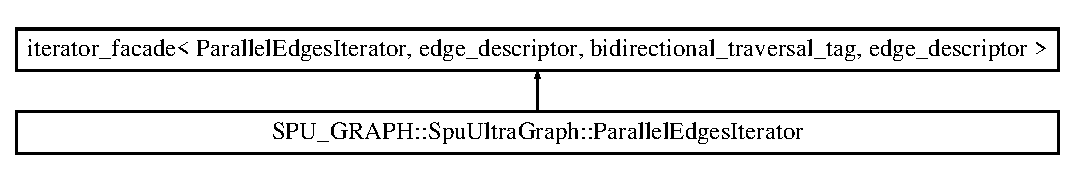
\includegraphics[height=1.839080cm]{class_s_p_u___g_r_a_p_h_1_1_spu_ultra_graph_1_1_parallel_edges_iterator}
\end{center}
\end{figure}
\doxysubsection*{Открытые члены}
\begin{DoxyCompactItemize}
\item 
\mbox{\Hypertarget{class_s_p_u___g_r_a_p_h_1_1_spu_ultra_graph_1_1_parallel_edges_iterator_a6cf06355aadbb64e98d33a0ebfa25209}\label{class_s_p_u___g_r_a_p_h_1_1_spu_ultra_graph_1_1_parallel_edges_iterator_a6cf06355aadbb64e98d33a0ebfa25209}} 
{\bfseries Parallel\+Edges\+Iterator} (const \mbox{\hyperlink{class_s_p_u___g_r_a_p_h_1_1_spu_ultra_graph}{Spu\+Ultra\+Graph}} $\ast$g, vertex\+\_\+descriptor from, vertex\+\_\+descriptor to, id\+\_\+t \mbox{\hyperlink{class_s_p_u___g_r_a_p_h_1_1_spu_ultra_graph_a51468aa2278d3abb0c338ffbeac7747a}{edge}}=0)
\item 
\mbox{\Hypertarget{class_s_p_u___g_r_a_p_h_1_1_spu_ultra_graph_1_1_parallel_edges_iterator_af9b4496f37517a45883e5e21d2d31d44}\label{class_s_p_u___g_r_a_p_h_1_1_spu_ultra_graph_1_1_parallel_edges_iterator_af9b4496f37517a45883e5e21d2d31d44}} 
\mbox{\hyperlink{class_s_p_u___g_r_a_p_h_1_1_spu_ultra_graph_a5f3776e003ef0a1648f1d9f84289810b}{edge\+\_\+descriptor}} {\bfseries dereference} () const
\item 
\mbox{\Hypertarget{class_s_p_u___g_r_a_p_h_1_1_spu_ultra_graph_1_1_parallel_edges_iterator_a8e1eb41f9082eb0140415ca3b4995d2e}\label{class_s_p_u___g_r_a_p_h_1_1_spu_ultra_graph_1_1_parallel_edges_iterator_a8e1eb41f9082eb0140415ca3b4995d2e}} 
bool {\bfseries equal} (const \mbox{\hyperlink{class_s_p_u___g_r_a_p_h_1_1_spu_ultra_graph_1_1_parallel_edges_iterator}{Parallel\+Edges\+Iterator}} \&other) const
\item 
\mbox{\Hypertarget{class_s_p_u___g_r_a_p_h_1_1_spu_ultra_graph_1_1_parallel_edges_iterator_a68f2818f6ea4a48761ba8f6fcbb3ee83}\label{class_s_p_u___g_r_a_p_h_1_1_spu_ultra_graph_1_1_parallel_edges_iterator_a68f2818f6ea4a48761ba8f6fcbb3ee83}} 
void {\bfseries increment} ()
\item 
\mbox{\Hypertarget{class_s_p_u___g_r_a_p_h_1_1_spu_ultra_graph_1_1_parallel_edges_iterator_a523f5ff4e4c5b3610bb81f8f8edfc6bd}\label{class_s_p_u___g_r_a_p_h_1_1_spu_ultra_graph_1_1_parallel_edges_iterator_a523f5ff4e4c5b3610bb81f8f8edfc6bd}} 
void {\bfseries decrement} ()
\end{DoxyCompactItemize}
\doxysubsection*{Друзья}
\begin{DoxyCompactItemize}
\item 
\mbox{\Hypertarget{class_s_p_u___g_r_a_p_h_1_1_spu_ultra_graph_1_1_parallel_edges_iterator_a0975271623c74c5b89bdf8d7fbce69c4}\label{class_s_p_u___g_r_a_p_h_1_1_spu_ultra_graph_1_1_parallel_edges_iterator_a0975271623c74c5b89bdf8d7fbce69c4}} 
class {\bfseries iterator\+\_\+core\+\_\+access}
\end{DoxyCompactItemize}


\doxysubsection{Подробное описание}
Итератор по параллельным ребрам от вершины from к to. 

Объявления и описания членов классов находятся в файлах\+:\begin{DoxyCompactItemize}
\item 
Spu\+Ultra\+Graph.\+h\item 
Spu\+Ultra\+Graph.\+cpp\end{DoxyCompactItemize}

\hypertarget{structboost_1_1property__map_3_01_spu_ultra_graph_00_01edge__all__t_01_4}{}\section{Шаблон структуры boost\+:\+:property\+\_\+map$<$ Spu\+Ultra\+Graph, edge\+\_\+all\+\_\+t $>$}
\label{structboost_1_1property__map_3_01_spu_ultra_graph_00_01edge__all__t_01_4}\index{boost\+::property\+\_\+map$<$ Spu\+Ultra\+Graph, edge\+\_\+all\+\_\+t $>$@{boost\+::property\+\_\+map$<$ Spu\+Ultra\+Graph, edge\+\_\+all\+\_\+t $>$}}
\subsection*{Открытые типы}
\begin{DoxyCompactItemize}
\item 
\mbox{\Hypertarget{structboost_1_1property__map_3_01_spu_ultra_graph_00_01edge__all__t_01_4_a3c9587a2e31d7bde52a169fb3f0947e1}\label{structboost_1_1property__map_3_01_spu_ultra_graph_00_01edge__all__t_01_4_a3c9587a2e31d7bde52a169fb3f0947e1}} 
typedef \hyperlink{classboost_1_1spu__ug__property__map}{spu\+\_\+ug\+\_\+edge\+\_\+data\+\_\+pm} {\bfseries type}
\item 
\mbox{\Hypertarget{structboost_1_1property__map_3_01_spu_ultra_graph_00_01edge__all__t_01_4_aeb3d171003be0e05d9f79a1787329e41}\label{structboost_1_1property__map_3_01_spu_ultra_graph_00_01edge__all__t_01_4_aeb3d171003be0e05d9f79a1787329e41}} 
typedef \hyperlink{classboost_1_1spu__ug__readable__property__map}{spu\+\_\+ug\+\_\+edge\+\_\+data\+\_\+pm\+\_\+const} {\bfseries const\+\_\+type}
\end{DoxyCompactItemize}


Объявления и описания членов структуры находятся в файле\+:\begin{DoxyCompactItemize}
\item 
Spu\+Ultra\+Graph\+Property.\+h\end{DoxyCompactItemize}

\hypertarget{structboost_1_1property__map_3_01_spu_ultra_graph_00_01edge__index__t_01_4}{}\section{Шаблон структуры boost\+:\+:property\+\_\+map$<$ Spu\+Ultra\+Graph, edge\+\_\+index\+\_\+t $>$}
\label{structboost_1_1property__map_3_01_spu_ultra_graph_00_01edge__index__t_01_4}\index{boost\+::property\+\_\+map$<$ Spu\+Ultra\+Graph, edge\+\_\+index\+\_\+t $>$@{boost\+::property\+\_\+map$<$ Spu\+Ultra\+Graph, edge\+\_\+index\+\_\+t $>$}}
\subsection*{Открытые типы}
\begin{DoxyCompactItemize}
\item 
\mbox{\Hypertarget{structboost_1_1property__map_3_01_spu_ultra_graph_00_01edge__index__t_01_4_a6e303c45da30037ee413ce26e7f39f19}\label{structboost_1_1property__map_3_01_spu_ultra_graph_00_01edge__index__t_01_4_a6e303c45da30037ee413ce26e7f39f19}} 
typedef \hyperlink{classboost_1_1spu__ug__readable__property__map}{spu\+\_\+ug\+\_\+edge\+\_\+id\+\_\+pm} {\bfseries const\+\_\+type}
\item 
\mbox{\Hypertarget{structboost_1_1property__map_3_01_spu_ultra_graph_00_01edge__index__t_01_4_ad59cc33d18bb1d4766416233f95353c9}\label{structboost_1_1property__map_3_01_spu_ultra_graph_00_01edge__index__t_01_4_ad59cc33d18bb1d4766416233f95353c9}} 
typedef \hyperlink{classboost_1_1spu__ug__readable__property__map}{const\+\_\+type} {\bfseries type}
\end{DoxyCompactItemize}


Объявления и описания членов структуры находятся в файле\+:\begin{DoxyCompactItemize}
\item 
Spu\+Ultra\+Graph\+Property.\+h\end{DoxyCompactItemize}

\hypertarget{structboost_1_1property__map_3_01_spu_ultra_graph_00_01edge__weight__t_01_4}{}\section{Шаблон структуры boost\+:\+:property\+\_\+map$<$ Spu\+Ultra\+Graph, edge\+\_\+weight\+\_\+t $>$}
\label{structboost_1_1property__map_3_01_spu_ultra_graph_00_01edge__weight__t_01_4}\index{boost\+::property\+\_\+map$<$ Spu\+Ultra\+Graph, edge\+\_\+weight\+\_\+t $>$@{boost\+::property\+\_\+map$<$ Spu\+Ultra\+Graph, edge\+\_\+weight\+\_\+t $>$}}
\subsection*{Открытые типы}
\begin{DoxyCompactItemize}
\item 
\mbox{\Hypertarget{structboost_1_1property__map_3_01_spu_ultra_graph_00_01edge__weight__t_01_4_a202cfea1a28d0fdaa36d1acc9acea72b}\label{structboost_1_1property__map_3_01_spu_ultra_graph_00_01edge__weight__t_01_4_a202cfea1a28d0fdaa36d1acc9acea72b}} 
typedef \hyperlink{classboost_1_1spu__ug__readable__property__map}{spu\+\_\+ug\+\_\+weight\+\_\+pm} {\bfseries const\+\_\+type}
\item 
\mbox{\Hypertarget{structboost_1_1property__map_3_01_spu_ultra_graph_00_01edge__weight__t_01_4_a30ff842801eadeb5e6a19a26efe22237}\label{structboost_1_1property__map_3_01_spu_ultra_graph_00_01edge__weight__t_01_4_a30ff842801eadeb5e6a19a26efe22237}} 
typedef \hyperlink{classboost_1_1spu__ug__readable__property__map}{const\+\_\+type} {\bfseries type}
\end{DoxyCompactItemize}


Объявления и описания членов структуры находятся в файле\+:\begin{DoxyCompactItemize}
\item 
Spu\+Ultra\+Graph\+Property.\+h\end{DoxyCompactItemize}

\hypertarget{structboost_1_1property__map_3_01_spu_ultra_graph_00_01vertex__all__t_01_4}{}\doxysection{Структура boost\+::property\+\_\+map$<$ Spu\+Ultra\+Graph, vertex\+\_\+all\+\_\+t $>$}
\label{structboost_1_1property__map_3_01_spu_ultra_graph_00_01vertex__all__t_01_4}\index{boost::property\_map$<$ SpuUltraGraph, vertex\_all\_t $>$@{boost::property\_map$<$ SpuUltraGraph, vertex\_all\_t $>$}}
\doxysubsection*{Открытые типы}
\begin{DoxyCompactItemize}
\item 
\mbox{\Hypertarget{structboost_1_1property__map_3_01_spu_ultra_graph_00_01vertex__all__t_01_4_ada854241a377855e92b0d6e0e7ba2194}\label{structboost_1_1property__map_3_01_spu_ultra_graph_00_01vertex__all__t_01_4_ada854241a377855e92b0d6e0e7ba2194}} 
typedef \mbox{\hyperlink{classboost_1_1spu__ug__property__map}{spu\+\_\+ug\+\_\+vertex\+\_\+data\+\_\+pm}} {\bfseries type}
\item 
\mbox{\Hypertarget{structboost_1_1property__map_3_01_spu_ultra_graph_00_01vertex__all__t_01_4_a7c257c30104ecb41c254e61d6a356d7c}\label{structboost_1_1property__map_3_01_spu_ultra_graph_00_01vertex__all__t_01_4_a7c257c30104ecb41c254e61d6a356d7c}} 
typedef \mbox{\hyperlink{classboost_1_1spu__ug__readable__property__map}{spu\+\_\+ug\+\_\+vertex\+\_\+data\+\_\+pm\+\_\+const}} {\bfseries const\+\_\+type}
\end{DoxyCompactItemize}


Объявления и описания членов структуры находятся в файле\+:\begin{DoxyCompactItemize}
\item 
Spu\+Ultra\+Graph\+Property.\+h\end{DoxyCompactItemize}

\hypertarget{structboost_1_1property__map_3_01_spu_ultra_graph_00_01vertex__index__t_01_4}{}\doxysection{Структура boost\+::property\+\_\+map$<$ Spu\+Ultra\+Graph, vertex\+\_\+index\+\_\+t $>$}
\label{structboost_1_1property__map_3_01_spu_ultra_graph_00_01vertex__index__t_01_4}\index{boost::property\_map$<$ SpuUltraGraph, vertex\_index\_t $>$@{boost::property\_map$<$ SpuUltraGraph, vertex\_index\_t $>$}}
\doxysubsection*{Открытые типы}
\begin{DoxyCompactItemize}
\item 
\mbox{\Hypertarget{structboost_1_1property__map_3_01_spu_ultra_graph_00_01vertex__index__t_01_4_a6f4697da5aa31a486b43fbc7f15f9ca5}\label{structboost_1_1property__map_3_01_spu_ultra_graph_00_01vertex__index__t_01_4_a6f4697da5aa31a486b43fbc7f15f9ca5}} 
typedef \mbox{\hyperlink{classboost_1_1spu__ug__readable__property__map}{spu\+\_\+ug\+\_\+vertex\+\_\+id\+\_\+pm}} {\bfseries const\+\_\+type}
\item 
\mbox{\Hypertarget{structboost_1_1property__map_3_01_spu_ultra_graph_00_01vertex__index__t_01_4_ab7b15feec22f208ff59138675cd8402b}\label{structboost_1_1property__map_3_01_spu_ultra_graph_00_01vertex__index__t_01_4_ab7b15feec22f208ff59138675cd8402b}} 
typedef \mbox{\hyperlink{classboost_1_1spu__ug__readable__property__map}{const\+\_\+type}} {\bfseries type}
\end{DoxyCompactItemize}


Объявления и описания членов структуры находятся в файле\+:\begin{DoxyCompactItemize}
\item 
Spu\+Ultra\+Graph\+Property.\+h\end{DoxyCompactItemize}

\hypertarget{class_queue_error}{}\doxysection{Класс Queue\+Error}
\label{class_queue_error}\index{QueueError@{QueueError}}
Граф наследования\+:Queue\+Error\+:\begin{figure}[H]
\begin{center}
\leavevmode
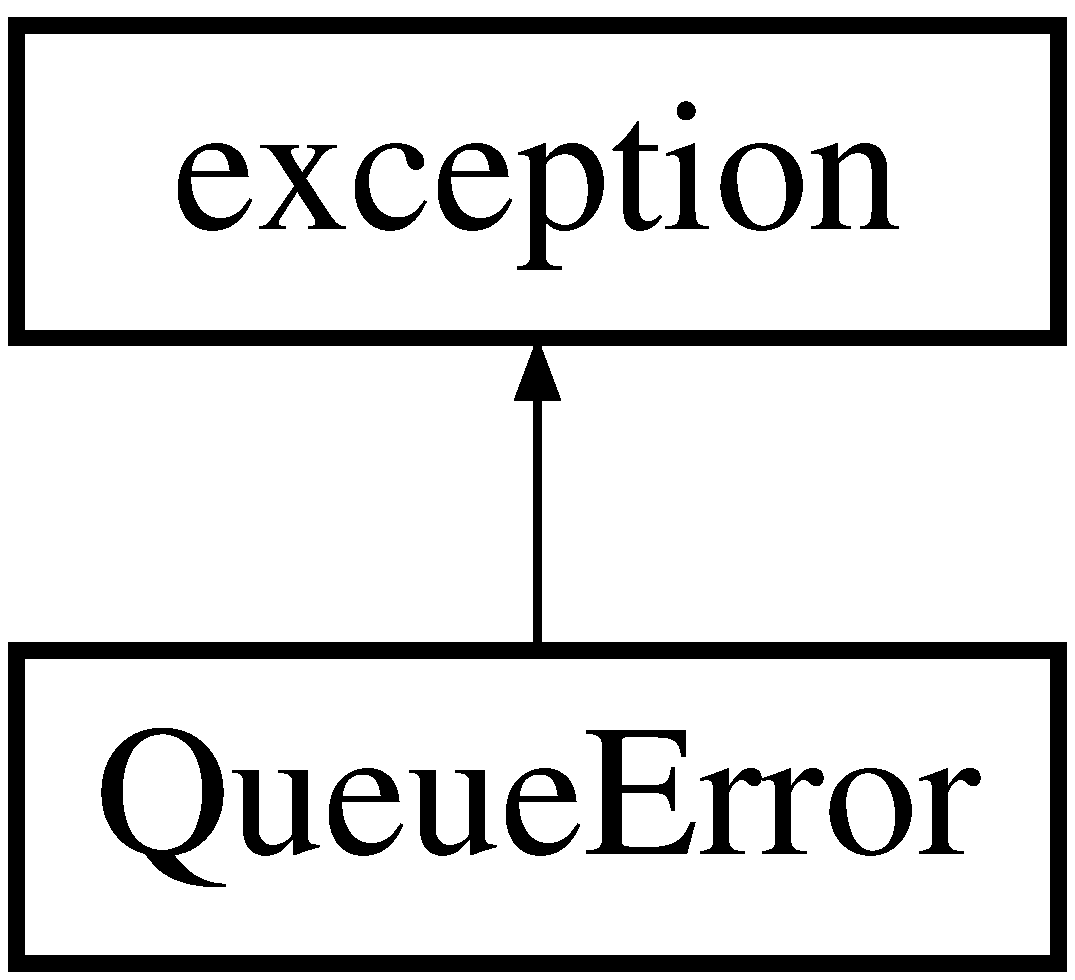
\includegraphics[height=2.000000cm]{class_queue_error}
\end{center}
\end{figure}
\doxysubsection*{Открытые члены}
\begin{DoxyCompactItemize}
\item 
\mbox{\Hypertarget{class_queue_error_a75b1c2766da17c9e1385c94caa0e5dfa}\label{class_queue_error_a75b1c2766da17c9e1385c94caa0e5dfa}} 
{\bfseries Queue\+Error} (const string \&error=\char`\"{}Queue error\char`\"{})
\item 
\mbox{\Hypertarget{class_queue_error_a7b8052680dcd81aeeb8e901d5698b2de}\label{class_queue_error_a7b8052680dcd81aeeb8e901d5698b2de}} 
const char $\ast$ {\bfseries what} () const noexcept override
\end{DoxyCompactItemize}


Объявления и описания членов класса находятся в файле\+:\begin{DoxyCompactItemize}
\item 
exceptions.\+h\end{DoxyCompactItemize}

\hypertarget{structrsltfrmt__0}{}\section{Структура rsltfrmt\+\_\+0}
\label{structrsltfrmt__0}\index{rsltfrmt\+\_\+0@{rsltfrmt\+\_\+0}}
\subsection*{Открытые атрибуты}
\begin{DoxyCompactItemize}
\item 
\mbox{\Hypertarget{structrsltfrmt__0_a717795d80df20b871c3db8998ab5c7a2}\label{structrsltfrmt__0_a717795d80df20b871c3db8998ab5c7a2}} 
rslt\+\_\+t {\bfseries rslt}
\item 
\mbox{\Hypertarget{structrsltfrmt__0_a6baad4340cc4fdf53078aa898cbe6441}\label{structrsltfrmt__0_a6baad4340cc4fdf53078aa898cbe6441}} 
\hyperlink{structgsid__container}{gsid\+\_\+t} {\bfseries gsid}
\end{DoxyCompactItemize}


Объявления и описания членов структуры находятся в файле\+:\begin{DoxyCompactItemize}
\item 
spu-\/api/libspu/spu.\+h\end{DoxyCompactItemize}

\hypertarget{structrsltfrmt__1}{}\section{Структура rsltfrmt\+\_\+1}
\label{structrsltfrmt__1}\index{rsltfrmt\+\_\+1@{rsltfrmt\+\_\+1}}
\subsection*{Открытые атрибуты}
\begin{DoxyCompactItemize}
\item 
\mbox{\Hypertarget{structrsltfrmt__1_ae8f0fe096836e4141fa183e1f685dc92}\label{structrsltfrmt__1_ae8f0fe096836e4141fa183e1f685dc92}} 
rslt\+\_\+t {\bfseries rslt}
\item 
\mbox{\Hypertarget{structrsltfrmt__1_a4c8f42801f1b448e7b5d321cc004c3ff}\label{structrsltfrmt__1_a4c8f42801f1b448e7b5d321cc004c3ff}} 
u32 {\bfseries power}
\end{DoxyCompactItemize}


Объявления и описания членов структуры находятся в файле\+:\begin{DoxyCompactItemize}
\item 
spu-\/api/libspu/spu.\+h\end{DoxyCompactItemize}

\hypertarget{structrsltfrmt__2}{}\section{Структура rsltfrmt\+\_\+2}
\label{structrsltfrmt__2}\index{rsltfrmt\+\_\+2@{rsltfrmt\+\_\+2}}
\subsection*{Открытые атрибуты}
\begin{DoxyCompactItemize}
\item 
\mbox{\Hypertarget{structrsltfrmt__2_a164b300126120520ac6dcb683760a378}\label{structrsltfrmt__2_a164b300126120520ac6dcb683760a378}} 
rslt\+\_\+t {\bfseries rslt}
\item 
\mbox{\Hypertarget{structrsltfrmt__2_af7a88ab2a952427cd8e4e5d80b3cebfd}\label{structrsltfrmt__2_af7a88ab2a952427cd8e4e5d80b3cebfd}} 
\hyperlink{structdata__container}{spu\+\_\+key\+\_\+t} {\bfseries key}
\item 
\mbox{\Hypertarget{structrsltfrmt__2_af6142a96e1b053960e2bf8586a30c5b8}\label{structrsltfrmt__2_af6142a96e1b053960e2bf8586a30c5b8}} 
\hyperlink{structdata__container}{val\+\_\+t} {\bfseries val}
\item 
\mbox{\Hypertarget{structrsltfrmt__2_ad104b51ce1d338934ad956116e40dbf4}\label{structrsltfrmt__2_ad104b51ce1d338934ad956116e40dbf4}} 
u32 {\bfseries power}
\end{DoxyCompactItemize}


Объявления и описания членов структуры находятся в файле\+:\begin{DoxyCompactItemize}
\item 
spu-\/api/libspu/spu.\+h\end{DoxyCompactItemize}

\hypertarget{classboost_1_1spu__ug__property__map}{}\section{Шаблон класса boost\+:\+:spu\+\_\+ug\+\_\+property\+\_\+map$<$ P\+R\+O\+P\+E\+R\+TY, V\+A\+L\+U\+E\+\_\+T $>$}
\label{classboost_1_1spu__ug__property__map}\index{boost\+::spu\+\_\+ug\+\_\+property\+\_\+map$<$ P\+R\+O\+P\+E\+R\+T\+Y, V\+A\+L\+U\+E\+\_\+\+T $>$@{boost\+::spu\+\_\+ug\+\_\+property\+\_\+map$<$ P\+R\+O\+P\+E\+R\+T\+Y, V\+A\+L\+U\+E\+\_\+\+T $>$}}
Граф наследования\+:boost\+:\+:spu\+\_\+ug\+\_\+property\+\_\+map$<$ P\+R\+O\+P\+E\+R\+TY, V\+A\+L\+U\+E\+\_\+T $>$\+:\begin{figure}[H]
\begin{center}
\leavevmode
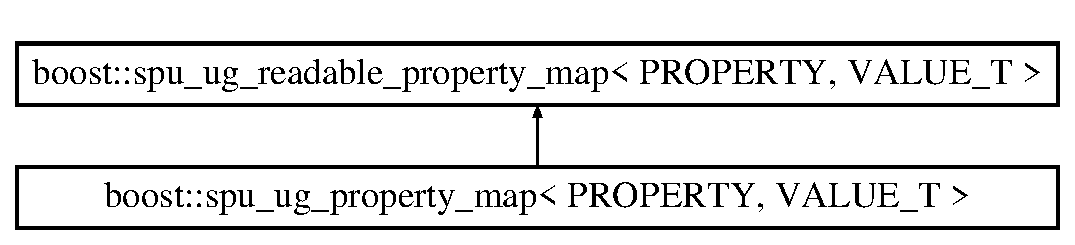
\includegraphics[height=2.000000cm]{classboost_1_1spu__ug__property__map}
\end{center}
\end{figure}
\subsection*{Открытые типы}
\begin{DoxyCompactItemize}
\item 
\mbox{\Hypertarget{classboost_1_1spu__ug__property__map_a40651558e7e4f89febe65f5b6eebcd19}\label{classboost_1_1spu__ug__property__map_a40651558e7e4f89febe65f5b6eebcd19}} 
typedef boost\+::read\+\_\+write\+\_\+property\+\_\+map\+\_\+tag {\bfseries category}
\end{DoxyCompactItemize}
\subsection*{Открытые члены}
\begin{DoxyCompactItemize}
\item 
\mbox{\Hypertarget{classboost_1_1spu__ug__property__map_a7820ea84ed846dabf4aecbb4d98eaf8a}\label{classboost_1_1spu__ug__property__map_a7820ea84ed846dabf4aecbb4d98eaf8a}} 
{\bfseries spu\+\_\+ug\+\_\+property\+\_\+map} (\hyperlink{class_s_p_u___g_r_a_p_h_1_1_spu_ultra_graph}{Spu\+Ultra\+Graph} $\ast$g)
\item 
\mbox{\Hypertarget{classboost_1_1spu__ug__property__map_a90c5fe6f7dfbba7bd3d54cc2dcab9f37}\label{classboost_1_1spu__ug__property__map_a90c5fe6f7dfbba7bd3d54cc2dcab9f37}} 
\hyperlink{class_s_p_u___g_r_a_p_h_1_1_spu_ultra_graph}{Spu\+Ultra\+Graph} $\ast$ {\bfseries get\+\_\+graph} () const
\end{DoxyCompactItemize}


Объявления и описания членов класса находятся в файле\+:\begin{DoxyCompactItemize}
\item 
Spu\+Ultra\+Graph\+Property.\+h\end{DoxyCompactItemize}

\hypertarget{classboost_1_1spu__ug__readable__property__map}{}\section{Шаблон класса boost\+:\+:spu\+\_\+ug\+\_\+readable\+\_\+property\+\_\+map$<$ P\+R\+O\+P\+E\+R\+TY, V\+A\+L\+U\+E\+\_\+T $>$}
\label{classboost_1_1spu__ug__readable__property__map}\index{boost\+::spu\+\_\+ug\+\_\+readable\+\_\+property\+\_\+map$<$ P\+R\+O\+P\+E\+R\+T\+Y, V\+A\+L\+U\+E\+\_\+\+T $>$@{boost\+::spu\+\_\+ug\+\_\+readable\+\_\+property\+\_\+map$<$ P\+R\+O\+P\+E\+R\+T\+Y, V\+A\+L\+U\+E\+\_\+\+T $>$}}
Граф наследования\+:boost\+:\+:spu\+\_\+ug\+\_\+readable\+\_\+property\+\_\+map$<$ P\+R\+O\+P\+E\+R\+TY, V\+A\+L\+U\+E\+\_\+T $>$\+:\begin{figure}[H]
\begin{center}
\leavevmode
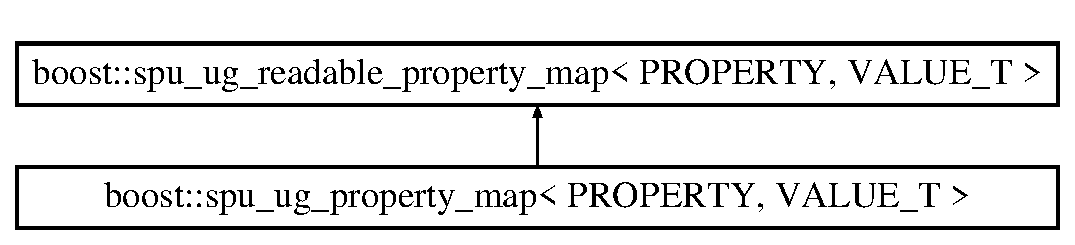
\includegraphics[height=2.000000cm]{classboost_1_1spu__ug__readable__property__map}
\end{center}
\end{figure}
\subsection*{Открытые типы}
\begin{DoxyCompactItemize}
\item 
\mbox{\Hypertarget{classboost_1_1spu__ug__readable__property__map_a36ae6d9c41a5bafe91283e3ec4104eed}\label{classboost_1_1spu__ug__readable__property__map_a36ae6d9c41a5bafe91283e3ec4104eed}} 
typedef boost\+::readable\+\_\+property\+\_\+map\+\_\+tag {\bfseries category}
\item 
\mbox{\Hypertarget{classboost_1_1spu__ug__readable__property__map_a251a71f41e97d7384ef97361ea10ddbc}\label{classboost_1_1spu__ug__readable__property__map_a251a71f41e97d7384ef97361ea10ddbc}} 
typedef V\+A\+L\+U\+E\+\_\+T {\bfseries value\+\_\+type}
\item 
\mbox{\Hypertarget{classboost_1_1spu__ug__readable__property__map_a996409eb98a3291d9890dd2fdb622e9b}\label{classboost_1_1spu__ug__readable__property__map_a996409eb98a3291d9890dd2fdb622e9b}} 
typedef V\+A\+L\+U\+E\+\_\+T {\bfseries reference}
\item 
\mbox{\Hypertarget{classboost_1_1spu__ug__readable__property__map_a9089a08c90f76368eb362bc8d8cbdb45}\label{classboost_1_1spu__ug__readable__property__map_a9089a08c90f76368eb362bc8d8cbdb45}} 
typedef S\+P\+U\+\_\+\+G\+R\+A\+P\+H\+::id\+\_\+t {\bfseries key\+\_\+type}
\end{DoxyCompactItemize}
\subsection*{Открытые члены}
\begin{DoxyCompactItemize}
\item 
\mbox{\Hypertarget{classboost_1_1spu__ug__readable__property__map_a67b585ee618ecf40930460ba4e03cb0d}\label{classboost_1_1spu__ug__readable__property__map_a67b585ee618ecf40930460ba4e03cb0d}} 
{\bfseries spu\+\_\+ug\+\_\+readable\+\_\+property\+\_\+map} (const \hyperlink{class_s_p_u___g_r_a_p_h_1_1_spu_ultra_graph}{Spu\+Ultra\+Graph} $\ast$g)
\item 
\mbox{\Hypertarget{classboost_1_1spu__ug__readable__property__map_a70019f5e3f097b0fc469235476fa18d3}\label{classboost_1_1spu__ug__readable__property__map_a70019f5e3f097b0fc469235476fa18d3}} 
const \hyperlink{class_s_p_u___g_r_a_p_h_1_1_spu_ultra_graph}{Spu\+Ultra\+Graph} $\ast$ {\bfseries get\+\_\+graph} () const
\end{DoxyCompactItemize}


Объявления и описания членов класса находятся в файле\+:\begin{DoxyCompactItemize}
\item 
Spu\+Ultra\+Graph\+Property.\+h\end{DoxyCompactItemize}

\hypertarget{struct_s_p_u___g_r_a_p_h_1_1_spu_ultra_graph_1_1spu__ultra__graph__traversal__category}{}\doxysection{Структура S\+P\+U\+\_\+\+G\+R\+A\+PH\+::Spu\+Ultra\+Graph\+::spu\+\_\+ultra\+\_\+graph\+\_\+traversal\+\_\+category}
\label{struct_s_p_u___g_r_a_p_h_1_1_spu_ultra_graph_1_1spu__ultra__graph__traversal__category}\index{SPU\_GRAPH::SpuUltraGraph::spu\_ultra\_graph\_traversal\_category@{SPU\_GRAPH::SpuUltraGraph::spu\_ultra\_graph\_traversal\_category}}


Категория обхода отражает поддерживаемые графовым классом виды итераторов  




{\ttfamily \#include $<$Spu\+Ultra\+Graph.\+h$>$}

Граф наследования\+:S\+P\+U\+\_\+\+G\+R\+A\+PH\+::Spu\+Ultra\+Graph\+::spu\+\_\+ultra\+\_\+graph\+\_\+traversal\+\_\+category\+:\begin{figure}[H]
\begin{center}
\leavevmode
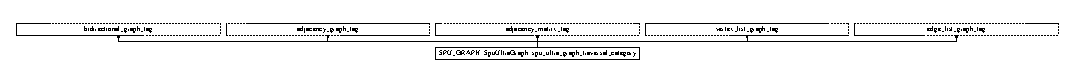
\includegraphics[height=0.567089cm]{struct_s_p_u___g_r_a_p_h_1_1_spu_ultra_graph_1_1spu__ultra__graph__traversal__category}
\end{center}
\end{figure}


\doxysubsection{Подробное описание}
Категория обхода отражает поддерживаемые графовым классом виды итераторов 

Объявления и описания членов структуры находятся в файле\+:\begin{DoxyCompactItemize}
\item 
Spu\+Ultra\+Graph.\+h\end{DoxyCompactItemize}

\hypertarget{class_s_p_u___g_r_a_p_h_1_1_spu_ultra_graph}{}\doxysection{Класс S\+P\+U\+\_\+\+G\+R\+A\+PH\+::Spu\+Ultra\+Graph}
\label{class_s_p_u___g_r_a_p_h_1_1_spu_ultra_graph}\index{SPU\_GRAPH::SpuUltraGraph@{SPU\_GRAPH::SpuUltraGraph}}
\doxysubsection*{Классы}
\begin{DoxyCompactItemize}
\item 
class \mbox{\hyperlink{class_s_p_u___g_r_a_p_h_1_1_spu_ultra_graph_1_1_adjacent_edges}{Adjacent\+Edges}}
\begin{DoxyCompactList}\small\item\em Контейнер содержащий смежные ребра для вершины v. \end{DoxyCompactList}\item 
class \mbox{\hyperlink{class_s_p_u___g_r_a_p_h_1_1_spu_ultra_graph_1_1_adjacent_edges_iterator}{Adjacent\+Edges\+Iterator}}
\item 
class \mbox{\hyperlink{class_s_p_u___g_r_a_p_h_1_1_spu_ultra_graph_1_1_adjacent_vertices}{Adjacent\+Vertices}}
\begin{DoxyCompactList}\small\item\em Контейнер содержащий вершины смежные вершине v. \end{DoxyCompactList}\item 
class \mbox{\hyperlink{class_s_p_u___g_r_a_p_h_1_1_spu_ultra_graph_1_1_adjacent_vertices_iterator}{Adjacent\+Vertices\+Iterator}}
\item 
class \mbox{\hyperlink{class_s_p_u___g_r_a_p_h_1_1_spu_ultra_graph_1_1_edge_iterator}{Edge\+Iterator}}
\item 
class \mbox{\hyperlink{class_s_p_u___g_r_a_p_h_1_1_spu_ultra_graph_1_1_edges}{Edges}}
\begin{DoxyCompactList}\small\item\em Контейнер содержащий все ребра графа \end{DoxyCompactList}\item 
class \mbox{\hyperlink{class_s_p_u___g_r_a_p_h_1_1_spu_ultra_graph_1_1_edge_vertices}{Edge\+Vertices}}
\begin{DoxyCompactList}\small\item\em Контейнер содержащий все источники для ребра e. \end{DoxyCompactList}\item 
class \mbox{\hyperlink{class_s_p_u___g_r_a_p_h_1_1_spu_ultra_graph_1_1_edge_vertices_iterator}{Edge\+Vertices\+Iterator}}
\begin{DoxyCompactList}\small\item\em Итератор по смежным вершинам для ребра e. \end{DoxyCompactList}\item 
class \mbox{\hyperlink{class_s_p_u___g_r_a_p_h_1_1_spu_ultra_graph_1_1_parallel_edges}{Parallel\+Edges}}
\begin{DoxyCompactList}\small\item\em Контейнер параллельных ребер от вершины from к to. \end{DoxyCompactList}\item 
class \mbox{\hyperlink{class_s_p_u___g_r_a_p_h_1_1_spu_ultra_graph_1_1_parallel_edges_iterator}{Parallel\+Edges\+Iterator}}
\begin{DoxyCompactList}\small\item\em Итератор по параллельным ребрам от вершины from к to. \end{DoxyCompactList}\item 
struct \mbox{\hyperlink{struct_s_p_u___g_r_a_p_h_1_1_spu_ultra_graph_1_1spu__ultra__graph__traversal__category}{spu\+\_\+ultra\+\_\+graph\+\_\+traversal\+\_\+category}}
\begin{DoxyCompactList}\small\item\em Категория обхода отражает поддерживаемые графовым классом виды итераторов \end{DoxyCompactList}\item 
class \mbox{\hyperlink{class_s_p_u___g_r_a_p_h_1_1_spu_ultra_graph_1_1_vertex_iterator}{Vertex\+Iterator}}
\item 
class \mbox{\hyperlink{class_s_p_u___g_r_a_p_h_1_1_spu_ultra_graph_1_1_vertices}{Vertices}}
\begin{DoxyCompactList}\small\item\em Контейнер содержащий все ребра графа \end{DoxyCompactList}\end{DoxyCompactItemize}
\doxysubsection*{Открытые типы}
\begin{DoxyCompactItemize}
\item 
\mbox{\Hypertarget{class_s_p_u___g_r_a_p_h_1_1_spu_ultra_graph_ac639c2679b6d9547625dfe514b2c641d}\label{class_s_p_u___g_r_a_p_h_1_1_spu_ultra_graph_ac639c2679b6d9547625dfe514b2c641d}} 
typedef id\+\_\+t {\bfseries vertex\+\_\+descriptor}
\item 
\mbox{\Hypertarget{class_s_p_u___g_r_a_p_h_1_1_spu_ultra_graph_a5f3776e003ef0a1648f1d9f84289810b}\label{class_s_p_u___g_r_a_p_h_1_1_spu_ultra_graph_a5f3776e003ef0a1648f1d9f84289810b}} 
typedef id\+\_\+t \mbox{\hyperlink{class_s_p_u___g_r_a_p_h_1_1_spu_ultra_graph_a5f3776e003ef0a1648f1d9f84289810b}{edge\+\_\+descriptor}}
\begin{DoxyCompactList}\small\item\em Тип объектов, используемых для идентификации ребер в графе. \end{DoxyCompactList}\item 
\mbox{\Hypertarget{class_s_p_u___g_r_a_p_h_1_1_spu_ultra_graph_ac9130a0489302bded920012c8810ac4a}\label{class_s_p_u___g_r_a_p_h_1_1_spu_ultra_graph_ac9130a0489302bded920012c8810ac4a}} 
typedef directed\+\_\+tag \mbox{\hyperlink{class_s_p_u___g_r_a_p_h_1_1_spu_ultra_graph_ac9130a0489302bded920012c8810ac4a}{directed\+\_\+category}}
\begin{DoxyCompactList}\small\item\em Предоставляет информацию о том, что граф ориентированный \end{DoxyCompactList}\item 
typedef allow\+\_\+parallel\+\_\+edge\+\_\+tag \mbox{\hyperlink{class_s_p_u___g_r_a_p_h_1_1_spu_ultra_graph_a6ae78f833e62e7fddd57b9c466e75255}{edge\+\_\+parallel\+\_\+category}}
\item 
\mbox{\Hypertarget{class_s_p_u___g_r_a_p_h_1_1_spu_ultra_graph_a489ed5ac88364fdac58607d539de975e}\label{class_s_p_u___g_r_a_p_h_1_1_spu_ultra_graph_a489ed5ac88364fdac58607d539de975e}} 
typedef \mbox{\hyperlink{struct_s_p_u___g_r_a_p_h_1_1_spu_ultra_graph_1_1spu__ultra__graph__traversal__category}{spu\+\_\+ultra\+\_\+graph\+\_\+traversal\+\_\+category}} \mbox{\hyperlink{class_s_p_u___g_r_a_p_h_1_1_spu_ultra_graph_a489ed5ac88364fdac58607d539de975e}{traversal\+\_\+category}}
\begin{DoxyCompactList}\small\item\em Категория обхода отражает поддерживаемые графовым классом виды итераторов \end{DoxyCompactList}\item 
\mbox{\Hypertarget{class_s_p_u___g_r_a_p_h_1_1_spu_ultra_graph_af8312efee580452b40e3750d8acf3b08}\label{class_s_p_u___g_r_a_p_h_1_1_spu_ultra_graph_af8312efee580452b40e3750d8acf3b08}} 
typedef size\+\_\+t \mbox{\hyperlink{class_s_p_u___g_r_a_p_h_1_1_spu_ultra_graph_af8312efee580452b40e3750d8acf3b08}{vertices\+\_\+size\+\_\+type}}
\begin{DoxyCompactList}\small\item\em Тип, используемый для представления числа вершин в графе \end{DoxyCompactList}\item 
\mbox{\Hypertarget{class_s_p_u___g_r_a_p_h_1_1_spu_ultra_graph_a82496f8d87c7dfab766f15a989a05aa4}\label{class_s_p_u___g_r_a_p_h_1_1_spu_ultra_graph_a82496f8d87c7dfab766f15a989a05aa4}} 
typedef size\+\_\+t \mbox{\hyperlink{class_s_p_u___g_r_a_p_h_1_1_spu_ultra_graph_a82496f8d87c7dfab766f15a989a05aa4}{edges\+\_\+size\+\_\+type}}
\begin{DoxyCompactList}\small\item\em Тип, используемый для представления числа ребер в графе \end{DoxyCompactList}\item 
\mbox{\Hypertarget{class_s_p_u___g_r_a_p_h_1_1_spu_ultra_graph_a0f24316ee9d0c5ea1b136cf4cf18c926}\label{class_s_p_u___g_r_a_p_h_1_1_spu_ultra_graph_a0f24316ee9d0c5ea1b136cf4cf18c926}} 
typedef size\+\_\+t \mbox{\hyperlink{class_s_p_u___g_r_a_p_h_1_1_spu_ultra_graph_a0f24316ee9d0c5ea1b136cf4cf18c926}{degree\+\_\+size\+\_\+type}}
\begin{DoxyCompactList}\small\item\em Тип, используемый для представления числа исходящих ребер в графе \end{DoxyCompactList}\item 
\mbox{\Hypertarget{class_s_p_u___g_r_a_p_h_1_1_spu_ultra_graph_a29b134691c15bbb48d3c213fa1492d49}\label{class_s_p_u___g_r_a_p_h_1_1_spu_ultra_graph_a29b134691c15bbb48d3c213fa1492d49}} 
typedef pair$<$ vertex\+\_\+descriptor, value\+\_\+t $>$ {\bfseries vertex\+\_\+property\+\_\+type}
\item 
\mbox{\Hypertarget{class_s_p_u___g_r_a_p_h_1_1_spu_ultra_graph_a2947d1a0c4a1e9bbb75e878511664127}\label{class_s_p_u___g_r_a_p_h_1_1_spu_ultra_graph_a2947d1a0c4a1e9bbb75e878511664127}} 
typedef pair$<$ vertex\+\_\+descriptor, value\+\_\+t $>$ {\bfseries edge\+\_\+property\+\_\+type}
\item 
\mbox{\Hypertarget{class_s_p_u___g_r_a_p_h_1_1_spu_ultra_graph_a06163cbc87b2e49334b4bcc46c7b0c89}\label{class_s_p_u___g_r_a_p_h_1_1_spu_ultra_graph_a06163cbc87b2e49334b4bcc46c7b0c89}} 
typedef \mbox{\hyperlink{class_s_p_u___g_r_a_p_h_1_1_spu_ultra_graph_1_1_vertex_iterator}{Vertex\+Iterator}} \mbox{\hyperlink{class_s_p_u___g_r_a_p_h_1_1_spu_ultra_graph_a06163cbc87b2e49334b4bcc46c7b0c89}{vertex\+\_\+iterator}}
\begin{DoxyCompactList}\small\item\em Итератор по всем вершинам \end{DoxyCompactList}\item 
\mbox{\Hypertarget{class_s_p_u___g_r_a_p_h_1_1_spu_ultra_graph_abf3933dd7a8c18410837fee58a8a8a10}\label{class_s_p_u___g_r_a_p_h_1_1_spu_ultra_graph_abf3933dd7a8c18410837fee58a8a8a10}} 
typedef \mbox{\hyperlink{class_s_p_u___g_r_a_p_h_1_1_spu_ultra_graph_1_1_edge_iterator}{Edge\+Iterator}} \mbox{\hyperlink{class_s_p_u___g_r_a_p_h_1_1_spu_ultra_graph_abf3933dd7a8c18410837fee58a8a8a10}{edge\+\_\+iterator}}
\begin{DoxyCompactList}\small\item\em Итератор по всем ребрам \end{DoxyCompactList}\item 
\mbox{\Hypertarget{class_s_p_u___g_r_a_p_h_1_1_spu_ultra_graph_adccd2b84a437514b4c5d341ccfea6f8b}\label{class_s_p_u___g_r_a_p_h_1_1_spu_ultra_graph_adccd2b84a437514b4c5d341ccfea6f8b}} 
typedef \mbox{\hyperlink{class_s_p_u___g_r_a_p_h_1_1_spu_ultra_graph_1_1_adjacent_edges_iterator}{Adjacent\+Edges\+Iterator}}$<$ 0 $>$ \mbox{\hyperlink{class_s_p_u___g_r_a_p_h_1_1_spu_ultra_graph_adccd2b84a437514b4c5d341ccfea6f8b}{out\+\_\+edge\+\_\+iterator}}
\begin{DoxyCompactList}\small\item\em Итератор по исходящим ребрам \end{DoxyCompactList}\item 
\mbox{\Hypertarget{class_s_p_u___g_r_a_p_h_1_1_spu_ultra_graph_ae658ac8b09fc1b84711e434354e027cd}\label{class_s_p_u___g_r_a_p_h_1_1_spu_ultra_graph_ae658ac8b09fc1b84711e434354e027cd}} 
typedef \mbox{\hyperlink{class_s_p_u___g_r_a_p_h_1_1_spu_ultra_graph_1_1_adjacent_edges_iterator}{Adjacent\+Edges\+Iterator}}$<$ 1 $>$ \mbox{\hyperlink{class_s_p_u___g_r_a_p_h_1_1_spu_ultra_graph_ae658ac8b09fc1b84711e434354e027cd}{in\+\_\+edge\+\_\+iterator}}
\begin{DoxyCompactList}\small\item\em Итератор по входящим ребрам \end{DoxyCompactList}\item 
\mbox{\Hypertarget{class_s_p_u___g_r_a_p_h_1_1_spu_ultra_graph_ae0fda272e54e0400446887572a5b4587}\label{class_s_p_u___g_r_a_p_h_1_1_spu_ultra_graph_ae0fda272e54e0400446887572a5b4587}} 
typedef \mbox{\hyperlink{class_s_p_u___g_r_a_p_h_1_1_spu_ultra_graph_1_1_adjacent_edges}{Adjacent\+Edges}}$<$ 0 $>$ \mbox{\hyperlink{class_s_p_u___g_r_a_p_h_1_1_spu_ultra_graph_ae0fda272e54e0400446887572a5b4587}{Out\+Edges}}
\begin{DoxyCompactList}\small\item\em Контейнер содержащий исходящие ребра для вершины v. \end{DoxyCompactList}\item 
\mbox{\Hypertarget{class_s_p_u___g_r_a_p_h_1_1_spu_ultra_graph_a3fc2875b9d11620ffa74cd83e544a95e}\label{class_s_p_u___g_r_a_p_h_1_1_spu_ultra_graph_a3fc2875b9d11620ffa74cd83e544a95e}} 
typedef \mbox{\hyperlink{class_s_p_u___g_r_a_p_h_1_1_spu_ultra_graph_1_1_adjacent_edges}{Adjacent\+Edges}}$<$ 1 $>$ \mbox{\hyperlink{class_s_p_u___g_r_a_p_h_1_1_spu_ultra_graph_a3fc2875b9d11620ffa74cd83e544a95e}{In\+Edges}}
\begin{DoxyCompactList}\small\item\em Контейнер содержащий входящие ребра для вершины v. \end{DoxyCompactList}\item 
\mbox{\Hypertarget{class_s_p_u___g_r_a_p_h_1_1_spu_ultra_graph_a417ef28fead78f635ab0a67d0bf5cef9}\label{class_s_p_u___g_r_a_p_h_1_1_spu_ultra_graph_a417ef28fead78f635ab0a67d0bf5cef9}} 
typedef \mbox{\hyperlink{class_s_p_u___g_r_a_p_h_1_1_spu_ultra_graph_1_1_edge_vertices_iterator}{Edge\+Vertices\+Iterator}}$<$ 0 $>$ \mbox{\hyperlink{class_s_p_u___g_r_a_p_h_1_1_spu_ultra_graph_a417ef28fead78f635ab0a67d0bf5cef9}{Source\+Iterator}}
\begin{DoxyCompactList}\small\item\em Итератор по источникам для ребра e. \end{DoxyCompactList}\item 
\mbox{\Hypertarget{class_s_p_u___g_r_a_p_h_1_1_spu_ultra_graph_a01da8848cb9d0515936072ad07187ce5}\label{class_s_p_u___g_r_a_p_h_1_1_spu_ultra_graph_a01da8848cb9d0515936072ad07187ce5}} 
typedef \mbox{\hyperlink{class_s_p_u___g_r_a_p_h_1_1_spu_ultra_graph_1_1_edge_vertices_iterator}{Edge\+Vertices\+Iterator}}$<$ 1 $>$ \mbox{\hyperlink{class_s_p_u___g_r_a_p_h_1_1_spu_ultra_graph_a01da8848cb9d0515936072ad07187ce5}{Target\+Iterator}}
\begin{DoxyCompactList}\small\item\em Итератор по стокам для ребра e. \end{DoxyCompactList}\item 
\mbox{\Hypertarget{class_s_p_u___g_r_a_p_h_1_1_spu_ultra_graph_affd7f90cfb9b255be603cb8756dfc80d}\label{class_s_p_u___g_r_a_p_h_1_1_spu_ultra_graph_affd7f90cfb9b255be603cb8756dfc80d}} 
typedef \mbox{\hyperlink{class_s_p_u___g_r_a_p_h_1_1_spu_ultra_graph_1_1_edge_vertices}{Edge\+Vertices}}$<$ 0 $>$ \mbox{\hyperlink{class_s_p_u___g_r_a_p_h_1_1_spu_ultra_graph_affd7f90cfb9b255be603cb8756dfc80d}{Sources}}
\begin{DoxyCompactList}\small\item\em Контейнер содержащий все источники для ребра e. \end{DoxyCompactList}\item 
\mbox{\Hypertarget{class_s_p_u___g_r_a_p_h_1_1_spu_ultra_graph_ae5b5d18bbcc112b25285ad2c06d32f07}\label{class_s_p_u___g_r_a_p_h_1_1_spu_ultra_graph_ae5b5d18bbcc112b25285ad2c06d32f07}} 
typedef \mbox{\hyperlink{class_s_p_u___g_r_a_p_h_1_1_spu_ultra_graph_1_1_edge_vertices}{Edge\+Vertices}}$<$ 1 $>$ \mbox{\hyperlink{class_s_p_u___g_r_a_p_h_1_1_spu_ultra_graph_ae5b5d18bbcc112b25285ad2c06d32f07}{Targets}}
\begin{DoxyCompactList}\small\item\em Контейнер содержащий все стоки для ребра e. \end{DoxyCompactList}\item 
\mbox{\Hypertarget{class_s_p_u___g_r_a_p_h_1_1_spu_ultra_graph_ae50dab54e277cf22d3e318d468e7585c}\label{class_s_p_u___g_r_a_p_h_1_1_spu_ultra_graph_ae50dab54e277cf22d3e318d468e7585c}} 
typedef \mbox{\hyperlink{class_s_p_u___g_r_a_p_h_1_1_spu_ultra_graph_1_1_adjacent_vertices_iterator}{Adjacent\+Vertices\+Iterator}} \mbox{\hyperlink{class_s_p_u___g_r_a_p_h_1_1_spu_ultra_graph_ae50dab54e277cf22d3e318d468e7585c}{adjacency\+\_\+iterator}}
\begin{DoxyCompactList}\small\item\em Итератор по смежным вершинам \end{DoxyCompactList}\end{DoxyCompactItemize}
\doxysubsection*{Открытые члены}
\begin{DoxyCompactItemize}
\item 
\mbox{\Hypertarget{class_s_p_u___g_r_a_p_h_1_1_spu_ultra_graph_a5092cab48140d2f7ce989555c118e783}\label{class_s_p_u___g_r_a_p_h_1_1_spu_ultra_graph_a5092cab48140d2f7ce989555c118e783}} 
{\bfseries Spu\+Ultra\+Graph} (id\+\_\+t graph\+\_\+id=0, const \mbox{\hyperlink{struct_s_p_u___g_r_a_p_h_1_1_spu_ultra_graph_traits}{Spu\+Ultra\+Graph\+Traits}} \&spu\+\_\+graph\+\_\+traits=\mbox{\hyperlink{struct_s_p_u___g_r_a_p_h_1_1_spu_ultra_graph_traits}{Spu\+Ultra\+Graph\+Traits}}())
\item 
\mbox{\Hypertarget{class_s_p_u___g_r_a_p_h_1_1_spu_ultra_graph_aedf362fe38b37dc25a7b028855718c25}\label{class_s_p_u___g_r_a_p_h_1_1_spu_ultra_graph_aedf362fe38b37dc25a7b028855718c25}} 
id\+\_\+t \mbox{\hyperlink{class_s_p_u___g_r_a_p_h_1_1_spu_ultra_graph_aedf362fe38b37dc25a7b028855718c25}{get\+\_\+id}} () const
\begin{DoxyCompactList}\small\item\em Возвращает id графа, определенного в структурах \end{DoxyCompactList}\item 
\mbox{\Hypertarget{class_s_p_u___g_r_a_p_h_1_1_spu_ultra_graph_ad4614b3f8123569a41a872141a1c5594}\label{class_s_p_u___g_r_a_p_h_1_1_spu_ultra_graph_ad4614b3f8123569a41a872141a1c5594}} 
id\+\_\+t \mbox{\hyperlink{class_s_p_u___g_r_a_p_h_1_1_spu_ultra_graph_ad4614b3f8123569a41a872141a1c5594}{get\+\_\+global\+\_\+id}} () const
\begin{DoxyCompactList}\small\item\em Возвращает глобальный id. Используется, например, для свойств графа. \end{DoxyCompactList}\item 
\mbox{\Hypertarget{class_s_p_u___g_r_a_p_h_1_1_spu_ultra_graph_a2b2210821bf0f6bce69fe8ec2756b2f7}\label{class_s_p_u___g_r_a_p_h_1_1_spu_ultra_graph_a2b2210821bf0f6bce69fe8ec2756b2f7}} 
vertex\+\_\+descriptor {\bfseries add\+\_\+vertex} ()
\item 
\mbox{\Hypertarget{class_s_p_u___g_r_a_p_h_1_1_spu_ultra_graph_a8c5c1c97abc61017a5e188cd7975e688}\label{class_s_p_u___g_r_a_p_h_1_1_spu_ultra_graph_a8c5c1c97abc61017a5e188cd7975e688}} 
vertex\+\_\+descriptor {\bfseries add\+\_\+vertex} (value\+\_\+t value)
\item 
\mbox{\Hypertarget{class_s_p_u___g_r_a_p_h_1_1_spu_ultra_graph_a0ab2bed50a562ddb4b3a3718cf7a50ab}\label{class_s_p_u___g_r_a_p_h_1_1_spu_ultra_graph_a0ab2bed50a562ddb4b3a3718cf7a50ab}} 
vertex\+\_\+descriptor {\bfseries add\+\_\+vertex} (vertex\+\_\+descriptor id)
\item 
\mbox{\Hypertarget{class_s_p_u___g_r_a_p_h_1_1_spu_ultra_graph_a66c63dc4bf4c8a47abd2974f4e16a83c}\label{class_s_p_u___g_r_a_p_h_1_1_spu_ultra_graph_a66c63dc4bf4c8a47abd2974f4e16a83c}} 
vertex\+\_\+descriptor {\bfseries add\+\_\+vertex} (vertex\+\_\+descriptor id, value\+\_\+t value)
\item 
void \mbox{\hyperlink{class_s_p_u___g_r_a_p_h_1_1_spu_ultra_graph_a70ef248cfbbebeda913dcde3507bb9ef}{put\+\_\+vertex}} (vertex\+\_\+descriptor id)
\item 
void \mbox{\hyperlink{class_s_p_u___g_r_a_p_h_1_1_spu_ultra_graph_a15f743f63444cd9cb8ecc1c9f611083f}{put\+\_\+vertex}} (vertex\+\_\+descriptor id, value\+\_\+t value)
\item 
\mbox{\Hypertarget{class_s_p_u___g_r_a_p_h_1_1_spu_ultra_graph_a981bb0adc93500e1650d9f2a4c0f023e}\label{class_s_p_u___g_r_a_p_h_1_1_spu_ultra_graph_a981bb0adc93500e1650d9f2a4c0f023e}} 
void {\bfseries remove\+\_\+vertex} (vertex\+\_\+descriptor v)
\item 
\mbox{\Hypertarget{class_s_p_u___g_r_a_p_h_1_1_spu_ultra_graph_a829d00276794f555b8620219f2f14be4}\label{class_s_p_u___g_r_a_p_h_1_1_spu_ultra_graph_a829d00276794f555b8620219f2f14be4}} 
bool {\bfseries has\+\_\+vertex} (vertex\+\_\+descriptor id) const
\item 
\mbox{\Hypertarget{class_s_p_u___g_r_a_p_h_1_1_spu_ultra_graph_a3815fc3e3cac1198e50ce271d6e67000}\label{class_s_p_u___g_r_a_p_h_1_1_spu_ultra_graph_a3815fc3e3cac1198e50ce271d6e67000}} 
\mbox{\hyperlink{class_s_p_u___g_r_a_p_h_1_1_spu_ultra_graph_af8312efee580452b40e3750d8acf3b08}{vertices\+\_\+size\+\_\+type}} {\bfseries num\+\_\+vertices} () const
\item 
\mbox{\Hypertarget{class_s_p_u___g_r_a_p_h_1_1_spu_ultra_graph_a998c3045e8f40869bdcc5a0f12199cd7}\label{class_s_p_u___g_r_a_p_h_1_1_spu_ultra_graph_a998c3045e8f40869bdcc5a0f12199cd7}} 
\mbox{\hyperlink{class_s_p_u___g_r_a_p_h_1_1_spu_ultra_graph_af8312efee580452b40e3750d8acf3b08}{vertices\+\_\+size\+\_\+type}} {\bfseries degree} (vertex\+\_\+descriptor v) const
\item 
\mbox{\Hypertarget{class_s_p_u___g_r_a_p_h_1_1_spu_ultra_graph_af5dfc7cb77da61beb1d30bfdd4658a92}\label{class_s_p_u___g_r_a_p_h_1_1_spu_ultra_graph_af5dfc7cb77da61beb1d30bfdd4658a92}} 
\mbox{\hyperlink{class_s_p_u___g_r_a_p_h_1_1_spu_ultra_graph_af8312efee580452b40e3750d8acf3b08}{vertices\+\_\+size\+\_\+type}} {\bfseries out\+\_\+degree} (vertex\+\_\+descriptor v) const
\item 
\mbox{\Hypertarget{class_s_p_u___g_r_a_p_h_1_1_spu_ultra_graph_a46cab7fb9993e412b5147a7c9e120273}\label{class_s_p_u___g_r_a_p_h_1_1_spu_ultra_graph_a46cab7fb9993e412b5147a7c9e120273}} 
\mbox{\hyperlink{class_s_p_u___g_r_a_p_h_1_1_spu_ultra_graph_af8312efee580452b40e3750d8acf3b08}{vertices\+\_\+size\+\_\+type}} {\bfseries in\+\_\+degree} (vertex\+\_\+descriptor v) const
\item 
void \mbox{\hyperlink{class_s_p_u___g_r_a_p_h_1_1_spu_ultra_graph_adf0f5b7b79b93ef295c39a615b51c71a}{clear\+\_\+vertex}} (vertex\+\_\+descriptor v, bool remove\+\_\+edges=true)
\item 
\mbox{\Hypertarget{class_s_p_u___g_r_a_p_h_1_1_spu_ultra_graph_ad8b9453c72f66fc00e2b2958a9670340}\label{class_s_p_u___g_r_a_p_h_1_1_spu_ultra_graph_ad8b9453c72f66fc00e2b2958a9670340}} 
void {\bfseries disconnect\+\_\+source} (vertex\+\_\+descriptor v, \mbox{\hyperlink{class_s_p_u___g_r_a_p_h_1_1_spu_ultra_graph_a5f3776e003ef0a1648f1d9f84289810b}{edge\+\_\+descriptor}} e)
\item 
\mbox{\Hypertarget{class_s_p_u___g_r_a_p_h_1_1_spu_ultra_graph_a896f0dd1c031841a9c16c03ed72235a0}\label{class_s_p_u___g_r_a_p_h_1_1_spu_ultra_graph_a896f0dd1c031841a9c16c03ed72235a0}} 
void {\bfseries disconnect\+\_\+target} (vertex\+\_\+descriptor v, \mbox{\hyperlink{class_s_p_u___g_r_a_p_h_1_1_spu_ultra_graph_a5f3776e003ef0a1648f1d9f84289810b}{edge\+\_\+descriptor}} e)
\item 
\mbox{\Hypertarget{class_s_p_u___g_r_a_p_h_1_1_spu_ultra_graph_a5d1dccd777a9686e72b775ebc3151936}\label{class_s_p_u___g_r_a_p_h_1_1_spu_ultra_graph_a5d1dccd777a9686e72b775ebc3151936}} 
\mbox{\hyperlink{class_s_p_u___g_r_a_p_h_1_1_spu_ultra_graph_a5f3776e003ef0a1648f1d9f84289810b}{edge\+\_\+descriptor}} {\bfseries add\+\_\+edge} ()
\item 
\mbox{\Hypertarget{class_s_p_u___g_r_a_p_h_1_1_spu_ultra_graph_a92ccccf0d18bd2dd146b605ae32a5ae1}\label{class_s_p_u___g_r_a_p_h_1_1_spu_ultra_graph_a92ccccf0d18bd2dd146b605ae32a5ae1}} 
\mbox{\hyperlink{class_s_p_u___g_r_a_p_h_1_1_spu_ultra_graph_a5f3776e003ef0a1648f1d9f84289810b}{edge\+\_\+descriptor}} {\bfseries add\+\_\+edge} (value\+\_\+t value)
\item 
\mbox{\Hypertarget{class_s_p_u___g_r_a_p_h_1_1_spu_ultra_graph_a74ca9423994b1dc3804d5fe62bb1a097}\label{class_s_p_u___g_r_a_p_h_1_1_spu_ultra_graph_a74ca9423994b1dc3804d5fe62bb1a097}} 
\mbox{\hyperlink{class_s_p_u___g_r_a_p_h_1_1_spu_ultra_graph_a5f3776e003ef0a1648f1d9f84289810b}{edge\+\_\+descriptor}} {\bfseries add\+\_\+edge} (\mbox{\hyperlink{class_s_p_u___g_r_a_p_h_1_1_spu_ultra_graph_a5f3776e003ef0a1648f1d9f84289810b}{edge\+\_\+descriptor}} id)
\item 
\mbox{\Hypertarget{class_s_p_u___g_r_a_p_h_1_1_spu_ultra_graph_a8a869529155dcb1e380f8fb3a16720ee}\label{class_s_p_u___g_r_a_p_h_1_1_spu_ultra_graph_a8a869529155dcb1e380f8fb3a16720ee}} 
\mbox{\hyperlink{class_s_p_u___g_r_a_p_h_1_1_spu_ultra_graph_a5f3776e003ef0a1648f1d9f84289810b}{edge\+\_\+descriptor}} {\bfseries add\+\_\+edge} (\mbox{\hyperlink{class_s_p_u___g_r_a_p_h_1_1_spu_ultra_graph_a5f3776e003ef0a1648f1d9f84289810b}{edge\+\_\+descriptor}} id, value\+\_\+t value)
\item 
\mbox{\Hypertarget{class_s_p_u___g_r_a_p_h_1_1_spu_ultra_graph_acf32b6a942095ea0c61b52b6596c8ecb}\label{class_s_p_u___g_r_a_p_h_1_1_spu_ultra_graph_acf32b6a942095ea0c61b52b6596c8ecb}} 
\mbox{\hyperlink{class_s_p_u___g_r_a_p_h_1_1_spu_ultra_graph_a5f3776e003ef0a1648f1d9f84289810b}{edge\+\_\+descriptor}} {\bfseries add\+\_\+edge} (vertex\+\_\+descriptor from, vertex\+\_\+descriptor to)
\item 
\mbox{\Hypertarget{class_s_p_u___g_r_a_p_h_1_1_spu_ultra_graph_a498c64e2dafbb4b294367ec325536b4f}\label{class_s_p_u___g_r_a_p_h_1_1_spu_ultra_graph_a498c64e2dafbb4b294367ec325536b4f}} 
\mbox{\hyperlink{class_s_p_u___g_r_a_p_h_1_1_spu_ultra_graph_a5f3776e003ef0a1648f1d9f84289810b}{edge\+\_\+descriptor}} {\bfseries add\+\_\+edge} (\mbox{\hyperlink{class_s_p_u___g_r_a_p_h_1_1_spu_ultra_graph_a5f3776e003ef0a1648f1d9f84289810b}{edge\+\_\+descriptor}} id, vertex\+\_\+descriptor from, vertex\+\_\+descriptor to)
\item 
\mbox{\Hypertarget{class_s_p_u___g_r_a_p_h_1_1_spu_ultra_graph_ab5389e1991a4c62b9da22b9dfd9e21f6}\label{class_s_p_u___g_r_a_p_h_1_1_spu_ultra_graph_ab5389e1991a4c62b9da22b9dfd9e21f6}} 
\mbox{\hyperlink{class_s_p_u___g_r_a_p_h_1_1_spu_ultra_graph_a5f3776e003ef0a1648f1d9f84289810b}{edge\+\_\+descriptor}} {\bfseries add\+\_\+edge} (\mbox{\hyperlink{class_s_p_u___g_r_a_p_h_1_1_spu_ultra_graph_a5f3776e003ef0a1648f1d9f84289810b}{edge\+\_\+descriptor}} id, vertex\+\_\+descriptor from, vertex\+\_\+descriptor to, value\+\_\+t value)
\item 
void \mbox{\hyperlink{class_s_p_u___g_r_a_p_h_1_1_spu_ultra_graph_a2039e0d5257d32c98a3207fdadb9f0b1}{put\+\_\+edge}} (\mbox{\hyperlink{class_s_p_u___g_r_a_p_h_1_1_spu_ultra_graph_a5f3776e003ef0a1648f1d9f84289810b}{edge\+\_\+descriptor}} id)
\item 
void \mbox{\hyperlink{class_s_p_u___g_r_a_p_h_1_1_spu_ultra_graph_a0688a06a76998bb616c6e8e97e86572c}{put\+\_\+edge}} (\mbox{\hyperlink{class_s_p_u___g_r_a_p_h_1_1_spu_ultra_graph_a5f3776e003ef0a1648f1d9f84289810b}{edge\+\_\+descriptor}} id, value\+\_\+t value)
\item 
\mbox{\Hypertarget{class_s_p_u___g_r_a_p_h_1_1_spu_ultra_graph_a545275ffcc2429db9496d89807d9235d}\label{class_s_p_u___g_r_a_p_h_1_1_spu_ultra_graph_a545275ffcc2429db9496d89807d9235d}} 
void {\bfseries add\+\_\+target} (\mbox{\hyperlink{class_s_p_u___g_r_a_p_h_1_1_spu_ultra_graph_a5f3776e003ef0a1648f1d9f84289810b}{edge\+\_\+descriptor}} \mbox{\hyperlink{class_s_p_u___g_r_a_p_h_1_1_spu_ultra_graph_a51468aa2278d3abb0c338ffbeac7747a}{edge}}, vertex\+\_\+descriptor vertex)
\item 
\mbox{\Hypertarget{class_s_p_u___g_r_a_p_h_1_1_spu_ultra_graph_ade233930d826a9bafdb6be51f62eaea4}\label{class_s_p_u___g_r_a_p_h_1_1_spu_ultra_graph_ade233930d826a9bafdb6be51f62eaea4}} 
void {\bfseries add\+\_\+source} (\mbox{\hyperlink{class_s_p_u___g_r_a_p_h_1_1_spu_ultra_graph_a5f3776e003ef0a1648f1d9f84289810b}{edge\+\_\+descriptor}} \mbox{\hyperlink{class_s_p_u___g_r_a_p_h_1_1_spu_ultra_graph_a51468aa2278d3abb0c338ffbeac7747a}{edge}}, vertex\+\_\+descriptor vertex)
\item 
\mbox{\Hypertarget{class_s_p_u___g_r_a_p_h_1_1_spu_ultra_graph_a19a04e44979bf73fb3cb8c84d4ba80f2}\label{class_s_p_u___g_r_a_p_h_1_1_spu_ultra_graph_a19a04e44979bf73fb3cb8c84d4ba80f2}} 
bool {\bfseries has\+\_\+edge} (\mbox{\hyperlink{class_s_p_u___g_r_a_p_h_1_1_spu_ultra_graph_a5f3776e003ef0a1648f1d9f84289810b}{edge\+\_\+descriptor}} id) const
\item 
\mbox{\Hypertarget{class_s_p_u___g_r_a_p_h_1_1_spu_ultra_graph_a2575209b0a91ff66d45554a9d3733eb9}\label{class_s_p_u___g_r_a_p_h_1_1_spu_ultra_graph_a2575209b0a91ff66d45554a9d3733eb9}} 
\mbox{\hyperlink{class_s_p_u___g_r_a_p_h_1_1_spu_ultra_graph_a5f3776e003ef0a1648f1d9f84289810b}{edge\+\_\+descriptor}} \mbox{\hyperlink{class_s_p_u___g_r_a_p_h_1_1_spu_ultra_graph_a2575209b0a91ff66d45554a9d3733eb9}{get\+\_\+free\+\_\+edge\+\_\+descriptor}} (weight\+\_\+t weight) const
\begin{DoxyCompactList}\small\item\em Возвращает свободный дискриптор ребра с определенным весом, для последующего добавления \end{DoxyCompactList}\item 
\mbox{\Hypertarget{class_s_p_u___g_r_a_p_h_1_1_spu_ultra_graph_a4c75efb2d557d1e54d9881e38a42bf9b}\label{class_s_p_u___g_r_a_p_h_1_1_spu_ultra_graph_a4c75efb2d557d1e54d9881e38a42bf9b}} 
\mbox{\hyperlink{class_s_p_u___g_r_a_p_h_1_1_spu_ultra_graph_a5f3776e003ef0a1648f1d9f84289810b}{edge\+\_\+descriptor}} {\bfseries get\+\_\+edge\+\_\+descriptor} (id\+\_\+t edge\+\_\+id) const
\item 
\mbox{\hyperlink{class_s_p_u___g_r_a_p_h_1_1_spu_ultra_graph_a5f3776e003ef0a1648f1d9f84289810b}{edge\+\_\+descriptor}} \mbox{\hyperlink{class_s_p_u___g_r_a_p_h_1_1_spu_ultra_graph_a42c69c77768c92f5b4c657289ef1b129}{get\+\_\+edge\+\_\+descriptor}} (id\+\_\+t edge\+\_\+id, weight\+\_\+t weight) const
\item 
\mbox{\Hypertarget{class_s_p_u___g_r_a_p_h_1_1_spu_ultra_graph_a74eeded7f53b4a4d18bd1519fcce8086}\label{class_s_p_u___g_r_a_p_h_1_1_spu_ultra_graph_a74eeded7f53b4a4d18bd1519fcce8086}} 
weight\+\_\+t \mbox{\hyperlink{class_s_p_u___g_r_a_p_h_1_1_spu_ultra_graph_a74eeded7f53b4a4d18bd1519fcce8086}{get\+\_\+weight}} (\mbox{\hyperlink{class_s_p_u___g_r_a_p_h_1_1_spu_ultra_graph_a5f3776e003ef0a1648f1d9f84289810b}{edge\+\_\+descriptor}} \mbox{\hyperlink{class_s_p_u___g_r_a_p_h_1_1_spu_ultra_graph_a51468aa2278d3abb0c338ffbeac7747a}{edge}}) const
\begin{DoxyCompactList}\small\item\em Получение веса ребра из edge\+\_\+descriptor. \end{DoxyCompactList}\item 
\mbox{\Hypertarget{class_s_p_u___g_r_a_p_h_1_1_spu_ultra_graph_ae7b8a89aa7b971f90018194e11e57c2b}\label{class_s_p_u___g_r_a_p_h_1_1_spu_ultra_graph_ae7b8a89aa7b971f90018194e11e57c2b}} 
\mbox{\hyperlink{class_s_p_u___g_r_a_p_h_1_1_spu_ultra_graph_a82496f8d87c7dfab766f15a989a05aa4}{edges\+\_\+size\+\_\+type}} {\bfseries num\+\_\+edges} () const
\item 
\mbox{\Hypertarget{class_s_p_u___g_r_a_p_h_1_1_spu_ultra_graph_aeb41721305bfef5dcff6311abbbda7ec}\label{class_s_p_u___g_r_a_p_h_1_1_spu_ultra_graph_aeb41721305bfef5dcff6311abbbda7ec}} 
\mbox{\hyperlink{class_s_p_u___g_r_a_p_h_1_1_spu_ultra_graph_a82496f8d87c7dfab766f15a989a05aa4}{edges\+\_\+size\+\_\+type}} {\bfseries source\+\_\+cnt} (\mbox{\hyperlink{class_s_p_u___g_r_a_p_h_1_1_spu_ultra_graph_a5f3776e003ef0a1648f1d9f84289810b}{edge\+\_\+descriptor}} e)
\item 
\mbox{\Hypertarget{class_s_p_u___g_r_a_p_h_1_1_spu_ultra_graph_a2f78492495fcda18c53902af7a8fe760}\label{class_s_p_u___g_r_a_p_h_1_1_spu_ultra_graph_a2f78492495fcda18c53902af7a8fe760}} 
\mbox{\hyperlink{class_s_p_u___g_r_a_p_h_1_1_spu_ultra_graph_a82496f8d87c7dfab766f15a989a05aa4}{edges\+\_\+size\+\_\+type}} {\bfseries target\+\_\+cnt} (\mbox{\hyperlink{class_s_p_u___g_r_a_p_h_1_1_spu_ultra_graph_a5f3776e003ef0a1648f1d9f84289810b}{edge\+\_\+descriptor}} e)
\item 
vertex\+\_\+descriptor \mbox{\hyperlink{class_s_p_u___g_r_a_p_h_1_1_spu_ultra_graph_a16ea4ca22965b3dae74ca8c17b130fd8}{source}} (\mbox{\hyperlink{class_s_p_u___g_r_a_p_h_1_1_spu_ultra_graph_a5f3776e003ef0a1648f1d9f84289810b}{edge\+\_\+descriptor}} e) const
\item 
vertex\+\_\+descriptor \mbox{\hyperlink{class_s_p_u___g_r_a_p_h_1_1_spu_ultra_graph_a08fadbb34b68b030cfa09bada3ca8f56}{target}} (\mbox{\hyperlink{class_s_p_u___g_r_a_p_h_1_1_spu_ultra_graph_a5f3776e003ef0a1648f1d9f84289810b}{edge\+\_\+descriptor}} e) const
\item 
\mbox{\Hypertarget{class_s_p_u___g_r_a_p_h_1_1_spu_ultra_graph_ad1cfb4a7f1b4fecc6b2ef5d3d3af39bc}\label{class_s_p_u___g_r_a_p_h_1_1_spu_ultra_graph_ad1cfb4a7f1b4fecc6b2ef5d3d3af39bc}} 
void {\bfseries remove\+\_\+edge} (\mbox{\hyperlink{class_s_p_u___g_r_a_p_h_1_1_spu_ultra_graph_a5f3776e003ef0a1648f1d9f84289810b}{edge\+\_\+descriptor}} \mbox{\hyperlink{class_s_p_u___g_r_a_p_h_1_1_spu_ultra_graph_a51468aa2278d3abb0c338ffbeac7747a}{edge}})
\item 
void \mbox{\hyperlink{class_s_p_u___g_r_a_p_h_1_1_spu_ultra_graph_a25193f9b7e0b9df947d8e9bc82da6fdf}{remove\+\_\+edge}} (vertex\+\_\+descriptor from, vertex\+\_\+descriptor to)
\item 
value\+\_\+t \mbox{\hyperlink{class_s_p_u___g_r_a_p_h_1_1_spu_ultra_graph_a3b4f0766c244af3081a37d61fdf2faae}{get\+\_\+vertex\+\_\+value}} (vertex\+\_\+descriptor v) const
\item 
value\+\_\+t \mbox{\hyperlink{class_s_p_u___g_r_a_p_h_1_1_spu_ultra_graph_aa508f7947fae83893eb2eacab3631ec2}{get\+\_\+edge\+\_\+value}} (\mbox{\hyperlink{class_s_p_u___g_r_a_p_h_1_1_spu_ultra_graph_a5f3776e003ef0a1648f1d9f84289810b}{edge\+\_\+descriptor}} e) const
\item 
\mbox{\hyperlink{class_s_p_u___g_r_a_p_h_1_1_spu_ultra_graph_a5f3776e003ef0a1648f1d9f84289810b}{edge\+\_\+descriptor}} \mbox{\hyperlink{class_s_p_u___g_r_a_p_h_1_1_spu_ultra_graph_a51468aa2278d3abb0c338ffbeac7747a}{edge}} (vertex\+\_\+descriptor from, vertex\+\_\+descriptor to) const
\item 
\mbox{\Hypertarget{class_s_p_u___g_r_a_p_h_1_1_spu_ultra_graph_ab2227b9c29b84b1fa6e2a10f11af5df6}\label{class_s_p_u___g_r_a_p_h_1_1_spu_ultra_graph_ab2227b9c29b84b1fa6e2a10f11af5df6}} 
\mbox{\hyperlink{class_s_p_u___g_r_a_p_h_1_1_spu_ultra_graph_1_1_vertices}{Vertices}} \mbox{\hyperlink{class_s_p_u___g_r_a_p_h_1_1_spu_ultra_graph_ab2227b9c29b84b1fa6e2a10f11af5df6}{vertices}} () const
\begin{DoxyCompactList}\small\item\em Возвращает контейнер содержащий все вершины графа \end{DoxyCompactList}\item 
\mbox{\Hypertarget{class_s_p_u___g_r_a_p_h_1_1_spu_ultra_graph_a54da90f2ff56cd153a0b23521316e24d}\label{class_s_p_u___g_r_a_p_h_1_1_spu_ultra_graph_a54da90f2ff56cd153a0b23521316e24d}} 
\mbox{\hyperlink{class_s_p_u___g_r_a_p_h_1_1_spu_ultra_graph_1_1_adjacent_vertices}{Adjacent\+Vertices}} \mbox{\hyperlink{class_s_p_u___g_r_a_p_h_1_1_spu_ultra_graph_a54da90f2ff56cd153a0b23521316e24d}{adjacent\+\_\+vertices}} (vertex\+\_\+descriptor v) const
\begin{DoxyCompactList}\small\item\em Возвращает контейнер содержащий вершины смежные вершине v. \end{DoxyCompactList}\item 
\mbox{\Hypertarget{class_s_p_u___g_r_a_p_h_1_1_spu_ultra_graph_a1d0b0fab46b32b8ffebd435f7e5ae835}\label{class_s_p_u___g_r_a_p_h_1_1_spu_ultra_graph_a1d0b0fab46b32b8ffebd435f7e5ae835}} 
\mbox{\hyperlink{class_s_p_u___g_r_a_p_h_1_1_spu_ultra_graph_affd7f90cfb9b255be603cb8756dfc80d}{Sources}} \mbox{\hyperlink{class_s_p_u___g_r_a_p_h_1_1_spu_ultra_graph_a1d0b0fab46b32b8ffebd435f7e5ae835}{sources}} (\mbox{\hyperlink{class_s_p_u___g_r_a_p_h_1_1_spu_ultra_graph_a5f3776e003ef0a1648f1d9f84289810b}{edge\+\_\+descriptor}} e) const
\begin{DoxyCompactList}\small\item\em Возвращает контейнер содержащий источники для ребра e. \end{DoxyCompactList}\item 
\mbox{\Hypertarget{class_s_p_u___g_r_a_p_h_1_1_spu_ultra_graph_ab298125c943a8cbd0ab7cc937e4ed837}\label{class_s_p_u___g_r_a_p_h_1_1_spu_ultra_graph_ab298125c943a8cbd0ab7cc937e4ed837}} 
\mbox{\hyperlink{class_s_p_u___g_r_a_p_h_1_1_spu_ultra_graph_ae5b5d18bbcc112b25285ad2c06d32f07}{Targets}} \mbox{\hyperlink{class_s_p_u___g_r_a_p_h_1_1_spu_ultra_graph_ab298125c943a8cbd0ab7cc937e4ed837}{targets}} (\mbox{\hyperlink{class_s_p_u___g_r_a_p_h_1_1_spu_ultra_graph_a5f3776e003ef0a1648f1d9f84289810b}{edge\+\_\+descriptor}} e) const
\begin{DoxyCompactList}\small\item\em Возвращает контейнер содержащий стоки для ребра e. \end{DoxyCompactList}\item 
\mbox{\Hypertarget{class_s_p_u___g_r_a_p_h_1_1_spu_ultra_graph_adcef05b6bc051e5d854ee6376539b084}\label{class_s_p_u___g_r_a_p_h_1_1_spu_ultra_graph_adcef05b6bc051e5d854ee6376539b084}} 
\mbox{\hyperlink{class_s_p_u___g_r_a_p_h_1_1_spu_ultra_graph_1_1_edges}{Edges}} \mbox{\hyperlink{class_s_p_u___g_r_a_p_h_1_1_spu_ultra_graph_adcef05b6bc051e5d854ee6376539b084}{edges}} () const
\begin{DoxyCompactList}\small\item\em Возвращает контейнер содержащий все ребра графа \end{DoxyCompactList}\item 
\mbox{\Hypertarget{class_s_p_u___g_r_a_p_h_1_1_spu_ultra_graph_a95e3d9d5f45f98173847d5a0254a4a1f}\label{class_s_p_u___g_r_a_p_h_1_1_spu_ultra_graph_a95e3d9d5f45f98173847d5a0254a4a1f}} 
\mbox{\hyperlink{class_s_p_u___g_r_a_p_h_1_1_spu_ultra_graph_1_1_parallel_edges}{Parallel\+Edges}} \mbox{\hyperlink{class_s_p_u___g_r_a_p_h_1_1_spu_ultra_graph_a95e3d9d5f45f98173847d5a0254a4a1f}{parallel\+\_\+edges}} (vertex\+\_\+descriptor from, vertex\+\_\+descriptor to) const
\begin{DoxyCompactList}\small\item\em Возвращает контейнер параллельных ребер от вершины from к to. \end{DoxyCompactList}\item 
\mbox{\Hypertarget{class_s_p_u___g_r_a_p_h_1_1_spu_ultra_graph_ab1bda5ef7eb9a69b09c044b3365ee4d4}\label{class_s_p_u___g_r_a_p_h_1_1_spu_ultra_graph_ab1bda5ef7eb9a69b09c044b3365ee4d4}} 
\mbox{\hyperlink{class_s_p_u___g_r_a_p_h_1_1_spu_ultra_graph_ae0fda272e54e0400446887572a5b4587}{Out\+Edges}} \mbox{\hyperlink{class_s_p_u___g_r_a_p_h_1_1_spu_ultra_graph_ab1bda5ef7eb9a69b09c044b3365ee4d4}{out\+\_\+edges}} (vertex\+\_\+descriptor v) const
\begin{DoxyCompactList}\small\item\em Возвращает контейнер исходящих ребер от вершины v. \end{DoxyCompactList}\item 
\mbox{\Hypertarget{class_s_p_u___g_r_a_p_h_1_1_spu_ultra_graph_a43c59a6f12d139a9bcf98e00e8c4297a}\label{class_s_p_u___g_r_a_p_h_1_1_spu_ultra_graph_a43c59a6f12d139a9bcf98e00e8c4297a}} 
\mbox{\hyperlink{class_s_p_u___g_r_a_p_h_1_1_spu_ultra_graph_a3fc2875b9d11620ffa74cd83e544a95e}{In\+Edges}} \mbox{\hyperlink{class_s_p_u___g_r_a_p_h_1_1_spu_ultra_graph_a43c59a6f12d139a9bcf98e00e8c4297a}{in\+\_\+edges}} (vertex\+\_\+descriptor v) const
\begin{DoxyCompactList}\small\item\em Возвращает контейнер исходящих ребер от вершины v. \end{DoxyCompactList}\item 
\mbox{\Hypertarget{class_s_p_u___g_r_a_p_h_1_1_spu_ultra_graph_af5d0c196f4acbc30f17a2444c384b8af}\label{class_s_p_u___g_r_a_p_h_1_1_spu_ultra_graph_af5d0c196f4acbc30f17a2444c384b8af}} 
void \mbox{\hyperlink{class_s_p_u___g_r_a_p_h_1_1_spu_ultra_graph_af5d0c196f4acbc30f17a2444c384b8af}{print\+\_\+vertex\+\_\+struct}} () const
\begin{DoxyCompactList}\small\item\em Метод для отладки. Распечатывает структуру vertex. \end{DoxyCompactList}\item 
\mbox{\Hypertarget{class_s_p_u___g_r_a_p_h_1_1_spu_ultra_graph_a3bb6913fcff6a6ea7571e7b3e338a6a7}\label{class_s_p_u___g_r_a_p_h_1_1_spu_ultra_graph_a3bb6913fcff6a6ea7571e7b3e338a6a7}} 
void \mbox{\hyperlink{class_s_p_u___g_r_a_p_h_1_1_spu_ultra_graph_a3bb6913fcff6a6ea7571e7b3e338a6a7}{print\+\_\+edge\+\_\+struct}} () const
\begin{DoxyCompactList}\small\item\em Метод для отладки. Распечатывает структуру edge. \end{DoxyCompactList}\end{DoxyCompactItemize}
\doxysubsection*{Защищенные члены}
\begin{DoxyCompactItemize}
\item 
\mbox{\Hypertarget{class_s_p_u___g_r_a_p_h_1_1_spu_ultra_graph_a82de737110404734e13195c78c00ec04}\label{class_s_p_u___g_r_a_p_h_1_1_spu_ultra_graph_a82de737110404734e13195c78c00ec04}} 
\mbox{\hyperlink{class_s_p_u_1_1_fields}{Fields}} {\bfseries vertex\+\_\+key} (id\+\_\+t vertex=0, uint8\+\_\+t incidence=0, id\+\_\+t \mbox{\hyperlink{class_s_p_u___g_r_a_p_h_1_1_spu_ultra_graph_a51468aa2278d3abb0c338ffbeac7747a}{edge}}=0) const
\item 
\mbox{\Hypertarget{class_s_p_u___g_r_a_p_h_1_1_spu_ultra_graph_ad38ed0654546e116eda62960688ab014}\label{class_s_p_u___g_r_a_p_h_1_1_spu_ultra_graph_ad38ed0654546e116eda62960688ab014}} 
\mbox{\hyperlink{class_s_p_u_1_1_fields}{Fields}} {\bfseries edge\+\_\+key} (id\+\_\+t \mbox{\hyperlink{class_s_p_u___g_r_a_p_h_1_1_spu_ultra_graph_a51468aa2278d3abb0c338ffbeac7747a}{edge}}=0, uint8\+\_\+t incidence=0, id\+\_\+t vertex=0) const
\item 
\mbox{\Hypertarget{class_s_p_u___g_r_a_p_h_1_1_spu_ultra_graph_a878dcbdf2ab86bae044145e890b5fb29}\label{class_s_p_u___g_r_a_p_h_1_1_spu_ultra_graph_a878dcbdf2ab86bae044145e890b5fb29}} 
\mbox{\hyperlink{class_s_p_u_1_1_fields}{Fields}} {\bfseries out\+\_\+degree\+\_\+key} (vertex\+\_\+descriptor v) const
\item 
\mbox{\Hypertarget{class_s_p_u___g_r_a_p_h_1_1_spu_ultra_graph_acf8c23a3fa97c2a426dd9ec551197cea}\label{class_s_p_u___g_r_a_p_h_1_1_spu_ultra_graph_acf8c23a3fa97c2a426dd9ec551197cea}} 
\mbox{\hyperlink{class_s_p_u_1_1_fields}{Fields}} {\bfseries in\+\_\+degree\+\_\+key} (vertex\+\_\+descriptor v) const
\item 
\mbox{\Hypertarget{class_s_p_u___g_r_a_p_h_1_1_spu_ultra_graph_aee27272166a6ffb584dea3409751ae40}\label{class_s_p_u___g_r_a_p_h_1_1_spu_ultra_graph_aee27272166a6ffb584dea3409751ae40}} 
\mbox{\hyperlink{class_s_p_u_1_1_fields}{Fields}} {\bfseries target\+\_\+cnt\+\_\+key} (\mbox{\hyperlink{class_s_p_u___g_r_a_p_h_1_1_spu_ultra_graph_a5f3776e003ef0a1648f1d9f84289810b}{edge\+\_\+descriptor}} e) const
\item 
\mbox{\Hypertarget{class_s_p_u___g_r_a_p_h_1_1_spu_ultra_graph_a8cbcd4e0e830f2d6b39965d111a74123}\label{class_s_p_u___g_r_a_p_h_1_1_spu_ultra_graph_a8cbcd4e0e830f2d6b39965d111a74123}} 
\mbox{\hyperlink{class_s_p_u_1_1_fields}{Fields}} {\bfseries source\+\_\+cnt\+\_\+key} (\mbox{\hyperlink{class_s_p_u___g_r_a_p_h_1_1_spu_ultra_graph_a5f3776e003ef0a1648f1d9f84289810b}{edge\+\_\+descriptor}} e) const
\item 
\mbox{\Hypertarget{class_s_p_u___g_r_a_p_h_1_1_spu_ultra_graph_ab737d34a76c1712bc84ca7990481d2fc}\label{class_s_p_u___g_r_a_p_h_1_1_spu_ultra_graph_ab737d34a76c1712bc84ca7990481d2fc}} 
id\+\_\+t {\bfseries max\+\_\+vertex\+\_\+id} () const
\item 
\mbox{\Hypertarget{class_s_p_u___g_r_a_p_h_1_1_spu_ultra_graph_a7a4e46b23fdaf3d3e51865a2b6812bce}\label{class_s_p_u___g_r_a_p_h_1_1_spu_ultra_graph_a7a4e46b23fdaf3d3e51865a2b6812bce}} 
id\+\_\+t {\bfseries max\+\_\+edge\+\_\+id} () const
\item 
\mbox{\Hypertarget{class_s_p_u___g_r_a_p_h_1_1_spu_ultra_graph_aab82648f43be4f893c946652d75d9009}\label{class_s_p_u___g_r_a_p_h_1_1_spu_ultra_graph_aab82648f43be4f893c946652d75d9009}} 
id\+\_\+t {\bfseries max\+\_\+weight} () const
\item 
\mbox{\Hypertarget{class_s_p_u___g_r_a_p_h_1_1_spu_ultra_graph_accb02121a50d69bf3f03d45aa2c904d6}\label{class_s_p_u___g_r_a_p_h_1_1_spu_ultra_graph_accb02121a50d69bf3f03d45aa2c904d6}} 
bool {\bfseries is\+\_\+vertex\+\_\+id\+\_\+valid} (id\+\_\+t id) const
\item 
\mbox{\Hypertarget{class_s_p_u___g_r_a_p_h_1_1_spu_ultra_graph_a40a9aef9c9a3a06bc0b7b50907ca813d}\label{class_s_p_u___g_r_a_p_h_1_1_spu_ultra_graph_a40a9aef9c9a3a06bc0b7b50907ca813d}} 
id\+\_\+t {\bfseries get\+\_\+free\+\_\+vertex\+\_\+id} ()
\item 
\mbox{\Hypertarget{class_s_p_u___g_r_a_p_h_1_1_spu_ultra_graph_a77f02ba5ba51856e46cb978d1c7eca76}\label{class_s_p_u___g_r_a_p_h_1_1_spu_ultra_graph_a77f02ba5ba51856e46cb978d1c7eca76}} 
\mbox{\hyperlink{class_s_p_u___g_r_a_p_h_1_1_spu_ultra_graph_af8312efee580452b40e3750d8acf3b08}{vertices\+\_\+size\+\_\+type}} {\bfseries inc\+\_\+vertexes\+\_\+cnt} ()
\item 
\mbox{\Hypertarget{class_s_p_u___g_r_a_p_h_1_1_spu_ultra_graph_a7284a29b119ca4c90cb9edd24afcdf43}\label{class_s_p_u___g_r_a_p_h_1_1_spu_ultra_graph_a7284a29b119ca4c90cb9edd24afcdf43}} 
\mbox{\hyperlink{class_s_p_u___g_r_a_p_h_1_1_spu_ultra_graph_af8312efee580452b40e3750d8acf3b08}{vertices\+\_\+size\+\_\+type}} {\bfseries dec\+\_\+vertexes\+\_\+cnt} ()
\item 
\mbox{\Hypertarget{class_s_p_u___g_r_a_p_h_1_1_spu_ultra_graph_a964caeb8a151b899a994b97ae728b4be}\label{class_s_p_u___g_r_a_p_h_1_1_spu_ultra_graph_a964caeb8a151b899a994b97ae728b4be}} 
\mbox{\hyperlink{class_s_p_u___g_r_a_p_h_1_1_spu_ultra_graph_af8312efee580452b40e3750d8acf3b08}{vertices\+\_\+size\+\_\+type}} {\bfseries inc\+\_\+out\+\_\+degree} (vertex\+\_\+descriptor v, \mbox{\hyperlink{class_s_p_u___g_r_a_p_h_1_1_spu_ultra_graph_af8312efee580452b40e3750d8acf3b08}{vertices\+\_\+size\+\_\+type}} val=1)
\item 
\mbox{\Hypertarget{class_s_p_u___g_r_a_p_h_1_1_spu_ultra_graph_a1360f8e031451bce54bb0a8dd2afbb1c}\label{class_s_p_u___g_r_a_p_h_1_1_spu_ultra_graph_a1360f8e031451bce54bb0a8dd2afbb1c}} 
\mbox{\hyperlink{class_s_p_u___g_r_a_p_h_1_1_spu_ultra_graph_af8312efee580452b40e3750d8acf3b08}{vertices\+\_\+size\+\_\+type}} {\bfseries dec\+\_\+out\+\_\+degree} (vertex\+\_\+descriptor v, \mbox{\hyperlink{class_s_p_u___g_r_a_p_h_1_1_spu_ultra_graph_af8312efee580452b40e3750d8acf3b08}{vertices\+\_\+size\+\_\+type}} val=1)
\item 
\mbox{\Hypertarget{class_s_p_u___g_r_a_p_h_1_1_spu_ultra_graph_afc32912c2c3bfa0a1f186525f30dc3d1}\label{class_s_p_u___g_r_a_p_h_1_1_spu_ultra_graph_afc32912c2c3bfa0a1f186525f30dc3d1}} 
\mbox{\hyperlink{class_s_p_u___g_r_a_p_h_1_1_spu_ultra_graph_af8312efee580452b40e3750d8acf3b08}{vertices\+\_\+size\+\_\+type}} {\bfseries inc\+\_\+in\+\_\+degree} (vertex\+\_\+descriptor v, \mbox{\hyperlink{class_s_p_u___g_r_a_p_h_1_1_spu_ultra_graph_af8312efee580452b40e3750d8acf3b08}{vertices\+\_\+size\+\_\+type}} val=1)
\item 
\mbox{\Hypertarget{class_s_p_u___g_r_a_p_h_1_1_spu_ultra_graph_af053863088fb04356c851771caeaca05}\label{class_s_p_u___g_r_a_p_h_1_1_spu_ultra_graph_af053863088fb04356c851771caeaca05}} 
\mbox{\hyperlink{class_s_p_u___g_r_a_p_h_1_1_spu_ultra_graph_af8312efee580452b40e3750d8acf3b08}{vertices\+\_\+size\+\_\+type}} {\bfseries dec\+\_\+in\+\_\+degree} (vertex\+\_\+descriptor v, \mbox{\hyperlink{class_s_p_u___g_r_a_p_h_1_1_spu_ultra_graph_af8312efee580452b40e3750d8acf3b08}{vertices\+\_\+size\+\_\+type}} val=1)
\item 
\mbox{\Hypertarget{class_s_p_u___g_r_a_p_h_1_1_spu_ultra_graph_a99e00909a2edb10ad81ac1e9057c1053}\label{class_s_p_u___g_r_a_p_h_1_1_spu_ultra_graph_a99e00909a2edb10ad81ac1e9057c1053}} 
vertex\+\_\+descriptor {\bfseries \+\_\+add\+\_\+vertex} (vertex\+\_\+descriptor id, value\+\_\+t value)
\item 
\mbox{\Hypertarget{class_s_p_u___g_r_a_p_h_1_1_spu_ultra_graph_a9df0d5f597fe51d49caa4e8f292fa20f}\label{class_s_p_u___g_r_a_p_h_1_1_spu_ultra_graph_a9df0d5f597fe51d49caa4e8f292fa20f}} 
\mbox{\hyperlink{class_s_p_u___g_r_a_p_h_1_1_spu_ultra_graph_a5f3776e003ef0a1648f1d9f84289810b}{edge\+\_\+descriptor}} {\bfseries \+\_\+add\+\_\+edge} (\mbox{\hyperlink{class_s_p_u___g_r_a_p_h_1_1_spu_ultra_graph_a5f3776e003ef0a1648f1d9f84289810b}{edge\+\_\+descriptor}} id, value\+\_\+t value)
\item 
\mbox{\Hypertarget{class_s_p_u___g_r_a_p_h_1_1_spu_ultra_graph_a4e5faafc5cc68bd20357de2d3d11ebc2}\label{class_s_p_u___g_r_a_p_h_1_1_spu_ultra_graph_a4e5faafc5cc68bd20357de2d3d11ebc2}} 
void {\bfseries \+\_\+add\+\_\+target} (\mbox{\hyperlink{class_s_p_u___g_r_a_p_h_1_1_spu_ultra_graph_a5f3776e003ef0a1648f1d9f84289810b}{edge\+\_\+descriptor}} \mbox{\hyperlink{class_s_p_u___g_r_a_p_h_1_1_spu_ultra_graph_a51468aa2278d3abb0c338ffbeac7747a}{edge}}, vertex\+\_\+descriptor vertex)
\item 
\mbox{\Hypertarget{class_s_p_u___g_r_a_p_h_1_1_spu_ultra_graph_a2434edd7a6f1b35ea9e67379a4c12ddd}\label{class_s_p_u___g_r_a_p_h_1_1_spu_ultra_graph_a2434edd7a6f1b35ea9e67379a4c12ddd}} 
void {\bfseries \+\_\+add\+\_\+source} (\mbox{\hyperlink{class_s_p_u___g_r_a_p_h_1_1_spu_ultra_graph_a5f3776e003ef0a1648f1d9f84289810b}{edge\+\_\+descriptor}} \mbox{\hyperlink{class_s_p_u___g_r_a_p_h_1_1_spu_ultra_graph_a51468aa2278d3abb0c338ffbeac7747a}{edge}}, vertex\+\_\+descriptor vertex)
\item 
\mbox{\Hypertarget{class_s_p_u___g_r_a_p_h_1_1_spu_ultra_graph_a53da0a5c180690322919dacfc635da8c}\label{class_s_p_u___g_r_a_p_h_1_1_spu_ultra_graph_a53da0a5c180690322919dacfc635da8c}} 
bool {\bfseries is\+\_\+edge\+\_\+id\+\_\+valid} (id\+\_\+t id) const
\item 
\mbox{\Hypertarget{class_s_p_u___g_r_a_p_h_1_1_spu_ultra_graph_a147a1360ecb5b9076f9d39fd8b535ae7}\label{class_s_p_u___g_r_a_p_h_1_1_spu_ultra_graph_a147a1360ecb5b9076f9d39fd8b535ae7}} 
id\+\_\+t {\bfseries get\+\_\+free\+\_\+edge\+\_\+id} ()
\item 
\mbox{\Hypertarget{class_s_p_u___g_r_a_p_h_1_1_spu_ultra_graph_a30fb4596eff47c3a37e4877ffccb673c}\label{class_s_p_u___g_r_a_p_h_1_1_spu_ultra_graph_a30fb4596eff47c3a37e4877ffccb673c}} 
void {\bfseries inc\+\_\+edges\+\_\+cnt} ()
\item 
\mbox{\Hypertarget{class_s_p_u___g_r_a_p_h_1_1_spu_ultra_graph_afcdcd8d58cb37290e5bb6463b41917b4}\label{class_s_p_u___g_r_a_p_h_1_1_spu_ultra_graph_afcdcd8d58cb37290e5bb6463b41917b4}} 
void {\bfseries dec\+\_\+edges\+\_\+cnt} ()
\item 
\mbox{\Hypertarget{class_s_p_u___g_r_a_p_h_1_1_spu_ultra_graph_afbba9ab825107d30abaad6ad755181dc}\label{class_s_p_u___g_r_a_p_h_1_1_spu_ultra_graph_afbba9ab825107d30abaad6ad755181dc}} 
\mbox{\hyperlink{class_s_p_u___g_r_a_p_h_1_1_spu_ultra_graph_a82496f8d87c7dfab766f15a989a05aa4}{edges\+\_\+size\+\_\+type}} {\bfseries inc\+\_\+target\+\_\+cnt} (\mbox{\hyperlink{class_s_p_u___g_r_a_p_h_1_1_spu_ultra_graph_a5f3776e003ef0a1648f1d9f84289810b}{edge\+\_\+descriptor}} e, \mbox{\hyperlink{class_s_p_u___g_r_a_p_h_1_1_spu_ultra_graph_a82496f8d87c7dfab766f15a989a05aa4}{edges\+\_\+size\+\_\+type}} val=1)
\item 
\mbox{\Hypertarget{class_s_p_u___g_r_a_p_h_1_1_spu_ultra_graph_aecd72c93789f6e72393bb4caa65f2890}\label{class_s_p_u___g_r_a_p_h_1_1_spu_ultra_graph_aecd72c93789f6e72393bb4caa65f2890}} 
\mbox{\hyperlink{class_s_p_u___g_r_a_p_h_1_1_spu_ultra_graph_a82496f8d87c7dfab766f15a989a05aa4}{edges\+\_\+size\+\_\+type}} {\bfseries dec\+\_\+target\+\_\+cnt} (\mbox{\hyperlink{class_s_p_u___g_r_a_p_h_1_1_spu_ultra_graph_a5f3776e003ef0a1648f1d9f84289810b}{edge\+\_\+descriptor}} e, \mbox{\hyperlink{class_s_p_u___g_r_a_p_h_1_1_spu_ultra_graph_a82496f8d87c7dfab766f15a989a05aa4}{edges\+\_\+size\+\_\+type}} val=1)
\item 
\mbox{\Hypertarget{class_s_p_u___g_r_a_p_h_1_1_spu_ultra_graph_a0c708ee126c83806d8bfacd380951f34}\label{class_s_p_u___g_r_a_p_h_1_1_spu_ultra_graph_a0c708ee126c83806d8bfacd380951f34}} 
\mbox{\hyperlink{class_s_p_u___g_r_a_p_h_1_1_spu_ultra_graph_a82496f8d87c7dfab766f15a989a05aa4}{edges\+\_\+size\+\_\+type}} {\bfseries inc\+\_\+source\+\_\+cnt} (\mbox{\hyperlink{class_s_p_u___g_r_a_p_h_1_1_spu_ultra_graph_a5f3776e003ef0a1648f1d9f84289810b}{edge\+\_\+descriptor}} e, \mbox{\hyperlink{class_s_p_u___g_r_a_p_h_1_1_spu_ultra_graph_a82496f8d87c7dfab766f15a989a05aa4}{edges\+\_\+size\+\_\+type}} val=1)
\item 
\mbox{\Hypertarget{class_s_p_u___g_r_a_p_h_1_1_spu_ultra_graph_ae846ac80c5e12c728da4b61406591448}\label{class_s_p_u___g_r_a_p_h_1_1_spu_ultra_graph_ae846ac80c5e12c728da4b61406591448}} 
\mbox{\hyperlink{class_s_p_u___g_r_a_p_h_1_1_spu_ultra_graph_a82496f8d87c7dfab766f15a989a05aa4}{edges\+\_\+size\+\_\+type}} {\bfseries dec\+\_\+source\+\_\+cnt} (\mbox{\hyperlink{class_s_p_u___g_r_a_p_h_1_1_spu_ultra_graph_a5f3776e003ef0a1648f1d9f84289810b}{edge\+\_\+descriptor}} e, \mbox{\hyperlink{class_s_p_u___g_r_a_p_h_1_1_spu_ultra_graph_a82496f8d87c7dfab766f15a989a05aa4}{edges\+\_\+size\+\_\+type}} val=1)
\item 
\mbox{\Hypertarget{class_s_p_u___g_r_a_p_h_1_1_spu_ultra_graph_a256800f8d21b759cb2b40f170cb7a808}\label{class_s_p_u___g_r_a_p_h_1_1_spu_ultra_graph_a256800f8d21b759cb2b40f170cb7a808}} 
bool {\bfseries is\+\_\+valid\+\_\+edge\+\_\+resp} (\mbox{\hyperlink{struct_s_p_u_1_1pair__containter}{pair\+\_\+t}} resp, \mbox{\hyperlink{class_s_p_u___g_r_a_p_h_1_1_spu_ultra_graph_a5f3776e003ef0a1648f1d9f84289810b}{edge\+\_\+descriptor}} \mbox{\hyperlink{class_s_p_u___g_r_a_p_h_1_1_spu_ultra_graph_a51468aa2278d3abb0c338ffbeac7747a}{edge}}, uint8\+\_\+t incidence=0) const
\end{DoxyCompactItemize}
\doxysubsection*{Защищенные статические члены}
\begin{DoxyCompactItemize}
\item 
\mbox{\Hypertarget{class_s_p_u___g_r_a_p_h_1_1_spu_ultra_graph_ab121f2ee5eaa47372394fe785ae80b43}\label{class_s_p_u___g_r_a_p_h_1_1_spu_ultra_graph_ab121f2ee5eaa47372394fe785ae80b43}} 
static id\+\_\+t {\bfseries get\+\_\+free\+\_\+global\+\_\+id} ()
\end{DoxyCompactItemize}


\doxysubsection{Определения типов}
\mbox{\Hypertarget{class_s_p_u___g_r_a_p_h_1_1_spu_ultra_graph_a6ae78f833e62e7fddd57b9c466e75255}\label{class_s_p_u___g_r_a_p_h_1_1_spu_ultra_graph_a6ae78f833e62e7fddd57b9c466e75255}} 
\index{SPU\_GRAPH::SpuUltraGraph@{SPU\_GRAPH::SpuUltraGraph}!edge\_parallel\_category@{edge\_parallel\_category}}
\index{edge\_parallel\_category@{edge\_parallel\_category}!SPU\_GRAPH::SpuUltraGraph@{SPU\_GRAPH::SpuUltraGraph}}
\doxysubsubsection{\texorpdfstring{edge\_parallel\_category}{edge\_parallel\_category}}
{\footnotesize\ttfamily typedef allow\+\_\+parallel\+\_\+edge\+\_\+tag \mbox{\hyperlink{class_s_p_u___g_r_a_p_h_1_1_spu_ultra_graph_a6ae78f833e62e7fddd57b9c466e75255}{S\+P\+U\+\_\+\+G\+R\+A\+P\+H\+::\+Spu\+Ultra\+Graph\+::edge\+\_\+parallel\+\_\+category}}}

Дает информацию о том, что граф позволяет вставку параллельных ребер (ребер, у которых одна и та же начальная и конечная вершины) 

\doxysubsection{Методы}
\mbox{\Hypertarget{class_s_p_u___g_r_a_p_h_1_1_spu_ultra_graph_adf0f5b7b79b93ef295c39a615b51c71a}\label{class_s_p_u___g_r_a_p_h_1_1_spu_ultra_graph_adf0f5b7b79b93ef295c39a615b51c71a}} 
\index{SPU\_GRAPH::SpuUltraGraph@{SPU\_GRAPH::SpuUltraGraph}!clear\_vertex@{clear\_vertex}}
\index{clear\_vertex@{clear\_vertex}!SPU\_GRAPH::SpuUltraGraph@{SPU\_GRAPH::SpuUltraGraph}}
\doxysubsubsection{\texorpdfstring{clear\_vertex()}{clear\_vertex()}}
{\footnotesize\ttfamily void S\+P\+U\+\_\+\+G\+R\+A\+P\+H\+::\+Spu\+Ultra\+Graph\+::clear\+\_\+vertex (\begin{DoxyParamCaption}\item[{Spu\+Ultra\+Graph\+::vertex\+\_\+descriptor}]{v,  }\item[{bool}]{remove\+\_\+edges = {\ttfamily true} }\end{DoxyParamCaption})}

Отсоединяет вершину v от всех ребер 
\begin{DoxyParams}{Аргументы}
{\em v} & Вершина \\
\hline
{\em remove\+\_\+edges} & При true если у ребра не останется вершин \char`\"{}источников\char`\"{} или \char`\"{}стоков\char`\"{}, то ребро будет удалено\\
\hline
\end{DoxyParams}
Отсоединяет вершину v от всех ребер Если после ребро не соединено ни с одной вершиной, то оно удаляется \mbox{\Hypertarget{class_s_p_u___g_r_a_p_h_1_1_spu_ultra_graph_a51468aa2278d3abb0c338ffbeac7747a}\label{class_s_p_u___g_r_a_p_h_1_1_spu_ultra_graph_a51468aa2278d3abb0c338ffbeac7747a}} 
\index{SPU\_GRAPH::SpuUltraGraph@{SPU\_GRAPH::SpuUltraGraph}!edge@{edge}}
\index{edge@{edge}!SPU\_GRAPH::SpuUltraGraph@{SPU\_GRAPH::SpuUltraGraph}}
\doxysubsubsection{\texorpdfstring{edge()}{edge()}}
{\footnotesize\ttfamily \mbox{\hyperlink{class_s_p_u___g_r_a_p_h_1_1_spu_ultra_graph_a5f3776e003ef0a1648f1d9f84289810b}{Spu\+Ultra\+Graph\+::edge\+\_\+descriptor}} S\+P\+U\+\_\+\+G\+R\+A\+P\+H\+::\+Spu\+Ultra\+Graph\+::edge (\begin{DoxyParamCaption}\item[{vertex\+\_\+descriptor}]{from,  }\item[{vertex\+\_\+descriptor}]{to }\end{DoxyParamCaption}) const}

Возвращает дескриптор первого найденного ребра от вершины from к to. Если ребра нет, то возвращается 0 \mbox{\Hypertarget{class_s_p_u___g_r_a_p_h_1_1_spu_ultra_graph_a42c69c77768c92f5b4c657289ef1b129}\label{class_s_p_u___g_r_a_p_h_1_1_spu_ultra_graph_a42c69c77768c92f5b4c657289ef1b129}} 
\index{SPU\_GRAPH::SpuUltraGraph@{SPU\_GRAPH::SpuUltraGraph}!get\_edge\_descriptor@{get\_edge\_descriptor}}
\index{get\_edge\_descriptor@{get\_edge\_descriptor}!SPU\_GRAPH::SpuUltraGraph@{SPU\_GRAPH::SpuUltraGraph}}
\doxysubsubsection{\texorpdfstring{get\_edge\_descriptor()}{get\_edge\_descriptor()}}
{\footnotesize\ttfamily \mbox{\hyperlink{class_s_p_u___g_r_a_p_h_1_1_spu_ultra_graph_a5f3776e003ef0a1648f1d9f84289810b}{Spu\+Ultra\+Graph\+::edge\+\_\+descriptor}} S\+P\+U\+\_\+\+G\+R\+A\+P\+H\+::\+Spu\+Ultra\+Graph\+::get\+\_\+edge\+\_\+descriptor (\begin{DoxyParamCaption}\item[{id\+\_\+t}]{edge\+\_\+id,  }\item[{weight\+\_\+t}]{weight }\end{DoxyParamCaption}) const}

Формирование edge\+\_\+descriptor из веса ребра и индекса Это необходимо, например, для добавления взвешенных ребер. 
\begin{DoxyParams}{Аргументы}
{\em edge\+\_\+id} & Индекс ребра. Это не id ребра. Как раз id ребра (edge\+\_\+descriptor) состоит из веса и индекса. \\
\hline
{\em weight} & Вес ребра \\
\hline
\end{DoxyParams}
\mbox{\Hypertarget{class_s_p_u___g_r_a_p_h_1_1_spu_ultra_graph_aa508f7947fae83893eb2eacab3631ec2}\label{class_s_p_u___g_r_a_p_h_1_1_spu_ultra_graph_aa508f7947fae83893eb2eacab3631ec2}} 
\index{SPU\_GRAPH::SpuUltraGraph@{SPU\_GRAPH::SpuUltraGraph}!get\_edge\_value@{get\_edge\_value}}
\index{get\_edge\_value@{get\_edge\_value}!SPU\_GRAPH::SpuUltraGraph@{SPU\_GRAPH::SpuUltraGraph}}
\doxysubsubsection{\texorpdfstring{get\_edge\_value()}{get\_edge\_value()}}
{\footnotesize\ttfamily value\+\_\+t S\+P\+U\+\_\+\+G\+R\+A\+P\+H\+::\+Spu\+Ultra\+Graph\+::get\+\_\+edge\+\_\+value (\begin{DoxyParamCaption}\item[{\mbox{\hyperlink{class_s_p_u___g_r_a_p_h_1_1_spu_ultra_graph_a5f3776e003ef0a1648f1d9f84289810b}{Spu\+Ultra\+Graph\+::edge\+\_\+descriptor}}}]{e }\end{DoxyParamCaption}) const}

Получить данные ребра 
\begin{DoxyExceptions}{Исключения}
{\em \mbox{\hyperlink{class_not_found}{Not\+Found}}} & если нет вершины e \\
\hline
\end{DoxyExceptions}
\mbox{\Hypertarget{class_s_p_u___g_r_a_p_h_1_1_spu_ultra_graph_a3b4f0766c244af3081a37d61fdf2faae}\label{class_s_p_u___g_r_a_p_h_1_1_spu_ultra_graph_a3b4f0766c244af3081a37d61fdf2faae}} 
\index{SPU\_GRAPH::SpuUltraGraph@{SPU\_GRAPH::SpuUltraGraph}!get\_vertex\_value@{get\_vertex\_value}}
\index{get\_vertex\_value@{get\_vertex\_value}!SPU\_GRAPH::SpuUltraGraph@{SPU\_GRAPH::SpuUltraGraph}}
\doxysubsubsection{\texorpdfstring{get\_vertex\_value()}{get\_vertex\_value()}}
{\footnotesize\ttfamily value\+\_\+t S\+P\+U\+\_\+\+G\+R\+A\+P\+H\+::\+Spu\+Ultra\+Graph\+::get\+\_\+vertex\+\_\+value (\begin{DoxyParamCaption}\item[{vertex\+\_\+descriptor}]{v }\end{DoxyParamCaption}) const}

Получить данные вершины 
\begin{DoxyExceptions}{Исключения}
{\em \mbox{\hyperlink{class_not_found}{Not\+Found}}} & если нет вершины v \\
\hline
\end{DoxyExceptions}
\mbox{\Hypertarget{class_s_p_u___g_r_a_p_h_1_1_spu_ultra_graph_a2039e0d5257d32c98a3207fdadb9f0b1}\label{class_s_p_u___g_r_a_p_h_1_1_spu_ultra_graph_a2039e0d5257d32c98a3207fdadb9f0b1}} 
\index{SPU\_GRAPH::SpuUltraGraph@{SPU\_GRAPH::SpuUltraGraph}!put\_edge@{put\_edge}}
\index{put\_edge@{put\_edge}!SPU\_GRAPH::SpuUltraGraph@{SPU\_GRAPH::SpuUltraGraph}}
\doxysubsubsection{\texorpdfstring{put\_edge()}{put\_edge()}\hspace{0.1cm}{\footnotesize\ttfamily [1/2]}}
{\footnotesize\ttfamily void S\+P\+U\+\_\+\+G\+R\+A\+P\+H\+::\+Spu\+Ultra\+Graph\+::put\+\_\+edge (\begin{DoxyParamCaption}\item[{\mbox{\hyperlink{class_s_p_u___g_r_a_p_h_1_1_spu_ultra_graph_a5f3776e003ef0a1648f1d9f84289810b}{Spu\+Ultra\+Graph\+::edge\+\_\+descriptor}}}]{id }\end{DoxyParamCaption})}

Добавляет ребро, если его нет 
\begin{DoxyParams}{Аргументы}
{\em id} & Идентификатор ребра \\
\hline
\end{DoxyParams}
\mbox{\Hypertarget{class_s_p_u___g_r_a_p_h_1_1_spu_ultra_graph_a0688a06a76998bb616c6e8e97e86572c}\label{class_s_p_u___g_r_a_p_h_1_1_spu_ultra_graph_a0688a06a76998bb616c6e8e97e86572c}} 
\index{SPU\_GRAPH::SpuUltraGraph@{SPU\_GRAPH::SpuUltraGraph}!put\_edge@{put\_edge}}
\index{put\_edge@{put\_edge}!SPU\_GRAPH::SpuUltraGraph@{SPU\_GRAPH::SpuUltraGraph}}
\doxysubsubsection{\texorpdfstring{put\_edge()}{put\_edge()}\hspace{0.1cm}{\footnotesize\ttfamily [2/2]}}
{\footnotesize\ttfamily void S\+P\+U\+\_\+\+G\+R\+A\+P\+H\+::\+Spu\+Ultra\+Graph\+::put\+\_\+edge (\begin{DoxyParamCaption}\item[{\mbox{\hyperlink{class_s_p_u___g_r_a_p_h_1_1_spu_ultra_graph_a5f3776e003ef0a1648f1d9f84289810b}{Spu\+Ultra\+Graph\+::edge\+\_\+descriptor}}}]{id,  }\item[{value\+\_\+t}]{value }\end{DoxyParamCaption})}

Изменяет value у ребра. Если ребра нет, то добавляет новое. 
\begin{DoxyParams}{Аргументы}
{\em id} & Идентификатор ребра \\
\hline
{\em value} & Новый value \\
\hline
\end{DoxyParams}
\mbox{\Hypertarget{class_s_p_u___g_r_a_p_h_1_1_spu_ultra_graph_a70ef248cfbbebeda913dcde3507bb9ef}\label{class_s_p_u___g_r_a_p_h_1_1_spu_ultra_graph_a70ef248cfbbebeda913dcde3507bb9ef}} 
\index{SPU\_GRAPH::SpuUltraGraph@{SPU\_GRAPH::SpuUltraGraph}!put\_vertex@{put\_vertex}}
\index{put\_vertex@{put\_vertex}!SPU\_GRAPH::SpuUltraGraph@{SPU\_GRAPH::SpuUltraGraph}}
\doxysubsubsection{\texorpdfstring{put\_vertex()}{put\_vertex()}\hspace{0.1cm}{\footnotesize\ttfamily [1/2]}}
{\footnotesize\ttfamily void S\+P\+U\+\_\+\+G\+R\+A\+P\+H\+::\+Spu\+Ultra\+Graph\+::put\+\_\+vertex (\begin{DoxyParamCaption}\item[{Spu\+Ultra\+Graph\+::vertex\+\_\+descriptor}]{id }\end{DoxyParamCaption})}

Добавляет вершину, если ее нет 
\begin{DoxyParams}{Аргументы}
{\em id} & Идентификатор вершины \\
\hline
\end{DoxyParams}
\mbox{\Hypertarget{class_s_p_u___g_r_a_p_h_1_1_spu_ultra_graph_a15f743f63444cd9cb8ecc1c9f611083f}\label{class_s_p_u___g_r_a_p_h_1_1_spu_ultra_graph_a15f743f63444cd9cb8ecc1c9f611083f}} 
\index{SPU\_GRAPH::SpuUltraGraph@{SPU\_GRAPH::SpuUltraGraph}!put\_vertex@{put\_vertex}}
\index{put\_vertex@{put\_vertex}!SPU\_GRAPH::SpuUltraGraph@{SPU\_GRAPH::SpuUltraGraph}}
\doxysubsubsection{\texorpdfstring{put\_vertex()}{put\_vertex()}\hspace{0.1cm}{\footnotesize\ttfamily [2/2]}}
{\footnotesize\ttfamily void S\+P\+U\+\_\+\+G\+R\+A\+P\+H\+::\+Spu\+Ultra\+Graph\+::put\+\_\+vertex (\begin{DoxyParamCaption}\item[{Spu\+Ultra\+Graph\+::vertex\+\_\+descriptor}]{id,  }\item[{value\+\_\+t}]{value }\end{DoxyParamCaption})}

Изменяет value у вершины. Если вершины нет, то добавляет новую. 
\begin{DoxyParams}{Аргументы}
{\em id} & Идентификатор вершины \\
\hline
{\em value} & Новый value \\
\hline
\end{DoxyParams}
\mbox{\Hypertarget{class_s_p_u___g_r_a_p_h_1_1_spu_ultra_graph_a25193f9b7e0b9df947d8e9bc82da6fdf}\label{class_s_p_u___g_r_a_p_h_1_1_spu_ultra_graph_a25193f9b7e0b9df947d8e9bc82da6fdf}} 
\index{SPU\_GRAPH::SpuUltraGraph@{SPU\_GRAPH::SpuUltraGraph}!remove\_edge@{remove\_edge}}
\index{remove\_edge@{remove\_edge}!SPU\_GRAPH::SpuUltraGraph@{SPU\_GRAPH::SpuUltraGraph}}
\doxysubsubsection{\texorpdfstring{remove\_edge()}{remove\_edge()}}
{\footnotesize\ttfamily void S\+P\+U\+\_\+\+G\+R\+A\+P\+H\+::\+Spu\+Ultra\+Graph\+::remove\+\_\+edge (\begin{DoxyParamCaption}\item[{Spu\+Ultra\+Graph\+::vertex\+\_\+descriptor}]{from,  }\item[{Spu\+Ultra\+Graph\+::vertex\+\_\+descriptor}]{to }\end{DoxyParamCaption})}

Удаляются все соединения от вершины from к to. Ребро удаляется, если кол-\/во вершин источников или стоков равно 0 \mbox{\Hypertarget{class_s_p_u___g_r_a_p_h_1_1_spu_ultra_graph_a16ea4ca22965b3dae74ca8c17b130fd8}\label{class_s_p_u___g_r_a_p_h_1_1_spu_ultra_graph_a16ea4ca22965b3dae74ca8c17b130fd8}} 
\index{SPU\_GRAPH::SpuUltraGraph@{SPU\_GRAPH::SpuUltraGraph}!source@{source}}
\index{source@{source}!SPU\_GRAPH::SpuUltraGraph@{SPU\_GRAPH::SpuUltraGraph}}
\doxysubsubsection{\texorpdfstring{source()}{source()}}
{\footnotesize\ttfamily Spu\+Ultra\+Graph\+::vertex\+\_\+descriptor S\+P\+U\+\_\+\+G\+R\+A\+P\+H\+::\+Spu\+Ultra\+Graph\+::source (\begin{DoxyParamCaption}\item[{\mbox{\hyperlink{class_s_p_u___g_r_a_p_h_1_1_spu_ultra_graph_a5f3776e003ef0a1648f1d9f84289810b}{Spu\+Ultra\+Graph\+::edge\+\_\+descriptor}}}]{e }\end{DoxyParamCaption}) const}

Возвращает первую вершину источник для ребра e Если источников, нет то вернет 0 \mbox{\Hypertarget{class_s_p_u___g_r_a_p_h_1_1_spu_ultra_graph_a08fadbb34b68b030cfa09bada3ca8f56}\label{class_s_p_u___g_r_a_p_h_1_1_spu_ultra_graph_a08fadbb34b68b030cfa09bada3ca8f56}} 
\index{SPU\_GRAPH::SpuUltraGraph@{SPU\_GRAPH::SpuUltraGraph}!target@{target}}
\index{target@{target}!SPU\_GRAPH::SpuUltraGraph@{SPU\_GRAPH::SpuUltraGraph}}
\doxysubsubsection{\texorpdfstring{target()}{target()}}
{\footnotesize\ttfamily Spu\+Ultra\+Graph\+::vertex\+\_\+descriptor S\+P\+U\+\_\+\+G\+R\+A\+P\+H\+::\+Spu\+Ultra\+Graph\+::target (\begin{DoxyParamCaption}\item[{\mbox{\hyperlink{class_s_p_u___g_r_a_p_h_1_1_spu_ultra_graph_a5f3776e003ef0a1648f1d9f84289810b}{Spu\+Ultra\+Graph\+::edge\+\_\+descriptor}}}]{e }\end{DoxyParamCaption}) const}

Возвращает первую вершину сток для ребра e Если стоков нет, то вернет 0 

Объявления и описания членов классов находятся в файлах\+:\begin{DoxyCompactItemize}
\item 
Spu\+Ultra\+Graph.\+h\item 
Spu\+Ultra\+Graph.\+cpp\end{DoxyCompactItemize}

\hypertarget{struct_s_p_u___g_r_a_p_h_1_1_spu_ultra_graph_traits}{}\section{Структура S\+P\+U\+\_\+\+G\+R\+A\+PH\+:\+:Spu\+Ultra\+Graph\+Traits}
\label{struct_s_p_u___g_r_a_p_h_1_1_spu_ultra_graph_traits}\index{S\+P\+U\+\_\+\+G\+R\+A\+P\+H\+::\+Spu\+Ultra\+Graph\+Traits@{S\+P\+U\+\_\+\+G\+R\+A\+P\+H\+::\+Spu\+Ultra\+Graph\+Traits}}
\subsection*{Открытые члены}
\begin{DoxyCompactItemize}
\item 
\mbox{\Hypertarget{struct_s_p_u___g_r_a_p_h_1_1_spu_ultra_graph_traits_a8dfb5c8586fa1c4a45758792dbdf8307}\label{struct_s_p_u___g_r_a_p_h_1_1_spu_ultra_graph_traits_a8dfb5c8586fa1c4a45758792dbdf8307}} 
{\bfseries Spu\+Ultra\+Graph\+Traits} (\hyperlink{class_s_p_u___g_r_a_p_h_1_1_graph_structure}{Graph\+Structure} vertex\+\_\+structure, \hyperlink{class_s_p_u___g_r_a_p_h_1_1_graph_structure}{Graph\+Structure} edge\+\_\+structure)
\item 
\mbox{\Hypertarget{struct_s_p_u___g_r_a_p_h_1_1_spu_ultra_graph_traits_a3b534d027aa8a6ab62fa33b43f0cddb8}\label{struct_s_p_u___g_r_a_p_h_1_1_spu_ultra_graph_traits_a3b534d027aa8a6ab62fa33b43f0cddb8}} 
size\+\_\+t {\bfseries depth\+\_\+sum} ()
\end{DoxyCompactItemize}
\subsection*{Открытые атрибуты}
\begin{DoxyCompactItemize}
\item 
\mbox{\Hypertarget{struct_s_p_u___g_r_a_p_h_1_1_spu_ultra_graph_traits_ac6d36f5d0ed425710df5be62a118f246}\label{struct_s_p_u___g_r_a_p_h_1_1_spu_ultra_graph_traits_ac6d36f5d0ed425710df5be62a118f246}} 
\hyperlink{class_s_p_u___g_r_a_p_h_1_1_graph_structure}{Graph\+Structure} {\bfseries vertex\+\_\+struct}
\item 
\mbox{\Hypertarget{struct_s_p_u___g_r_a_p_h_1_1_spu_ultra_graph_traits_a563b5a8e172263ff3b23574a2edfb46f}\label{struct_s_p_u___g_r_a_p_h_1_1_spu_ultra_graph_traits_a563b5a8e172263ff3b23574a2edfb46f}} 
\hyperlink{class_s_p_u___g_r_a_p_h_1_1_graph_structure}{Graph\+Structure} {\bfseries edge\+\_\+struct}
\item 
\mbox{\Hypertarget{struct_s_p_u___g_r_a_p_h_1_1_spu_ultra_graph_traits_af647e861e35133da6e0c0aca38ab6ac7}\label{struct_s_p_u___g_r_a_p_h_1_1_spu_ultra_graph_traits_af647e861e35133da6e0c0aca38ab6ac7}} 
size\+\_\+t \hyperlink{struct_s_p_u___g_r_a_p_h_1_1_spu_ultra_graph_traits_af647e861e35133da6e0c0aca38ab6ac7}{graph\+\_\+id\+\_\+depth} = 3
\begin{DoxyCompactList}\small\item\em Кол-\/во бит под id графа \end{DoxyCompactList}\item 
\mbox{\Hypertarget{struct_s_p_u___g_r_a_p_h_1_1_spu_ultra_graph_traits_a8ee6c58e31936df5a1c98ecbdf4e00ed}\label{struct_s_p_u___g_r_a_p_h_1_1_spu_ultra_graph_traits_a8ee6c58e31936df5a1c98ecbdf4e00ed}} 
size\+\_\+t \hyperlink{struct_s_p_u___g_r_a_p_h_1_1_spu_ultra_graph_traits_a8ee6c58e31936df5a1c98ecbdf4e00ed}{vertex\+\_\+id\+\_\+depth} = 28
\begin{DoxyCompactList}\small\item\em Кол-\/во бит под id вершины \end{DoxyCompactList}\item 
\mbox{\Hypertarget{struct_s_p_u___g_r_a_p_h_1_1_spu_ultra_graph_traits_ad8da6ee1527f0ced8ae14bf3ad3b7cb9}\label{struct_s_p_u___g_r_a_p_h_1_1_spu_ultra_graph_traits_ad8da6ee1527f0ced8ae14bf3ad3b7cb9}} 
size\+\_\+t \hyperlink{struct_s_p_u___g_r_a_p_h_1_1_spu_ultra_graph_traits_ad8da6ee1527f0ced8ae14bf3ad3b7cb9}{edge\+\_\+id\+\_\+depth} = 28
\begin{DoxyCompactList}\small\item\em Кол-\/во бит под индекс ребра (вес ребра не воходит в это число) \end{DoxyCompactList}\item 
\mbox{\Hypertarget{struct_s_p_u___g_r_a_p_h_1_1_spu_ultra_graph_traits_a2e7eef788286039f97344f682ba16138}\label{struct_s_p_u___g_r_a_p_h_1_1_spu_ultra_graph_traits_a2e7eef788286039f97344f682ba16138}} 
size\+\_\+t \hyperlink{struct_s_p_u___g_r_a_p_h_1_1_spu_ultra_graph_traits_a2e7eef788286039f97344f682ba16138}{weight\+\_\+depth} = 4
\begin{DoxyCompactList}\small\item\em Кол-\/во бит под вес ребра \end{DoxyCompactList}\item 
\mbox{\Hypertarget{struct_s_p_u___g_r_a_p_h_1_1_spu_ultra_graph_traits_a6b9fee19a36b2f83c7cfc98b1067647b}\label{struct_s_p_u___g_r_a_p_h_1_1_spu_ultra_graph_traits_a6b9fee19a36b2f83c7cfc98b1067647b}} 
data\+\_\+t {\bfseries default\+\_\+vertex\+\_\+value} = 0
\item 
\mbox{\Hypertarget{struct_s_p_u___g_r_a_p_h_1_1_spu_ultra_graph_traits_accc2d70f8bb9550d7371b9465c9bb9fb}\label{struct_s_p_u___g_r_a_p_h_1_1_spu_ultra_graph_traits_accc2d70f8bb9550d7371b9465c9bb9fb}} 
data\+\_\+t {\bfseries default\+\_\+edge\+\_\+value} = 0
\item 
\mbox{\Hypertarget{struct_s_p_u___g_r_a_p_h_1_1_spu_ultra_graph_traits_a46908d59da7ab7b6b40e26514479dcf1}\label{struct_s_p_u___g_r_a_p_h_1_1_spu_ultra_graph_traits_a46908d59da7ab7b6b40e26514479dcf1}} 
data\+\_\+t {\bfseries default\+\_\+weight} = 0
\end{DoxyCompactItemize}


Объявления и описания членов структуры находятся в файле\+:\begin{DoxyCompactItemize}
\item 
Spu\+Ultra\+Graph.\+h\end{DoxyCompactItemize}

\hypertarget{class_s_p_u_1_1_structure}{}\section{Шаблон класса S\+PU\+:\+:Structure$<$ Key\+NameT, Value\+NameT $>$}
\label{class_s_p_u_1_1_structure}\index{S\+P\+U\+::\+Structure$<$ Key\+Name\+T, Value\+Name\+T $>$@{S\+P\+U\+::\+Structure$<$ Key\+Name\+T, Value\+Name\+T $>$}}
Граф наследования\+:S\+PU\+:\+:Structure$<$ Key\+NameT, Value\+NameT $>$\+:\begin{figure}[H]
\begin{center}
\leavevmode
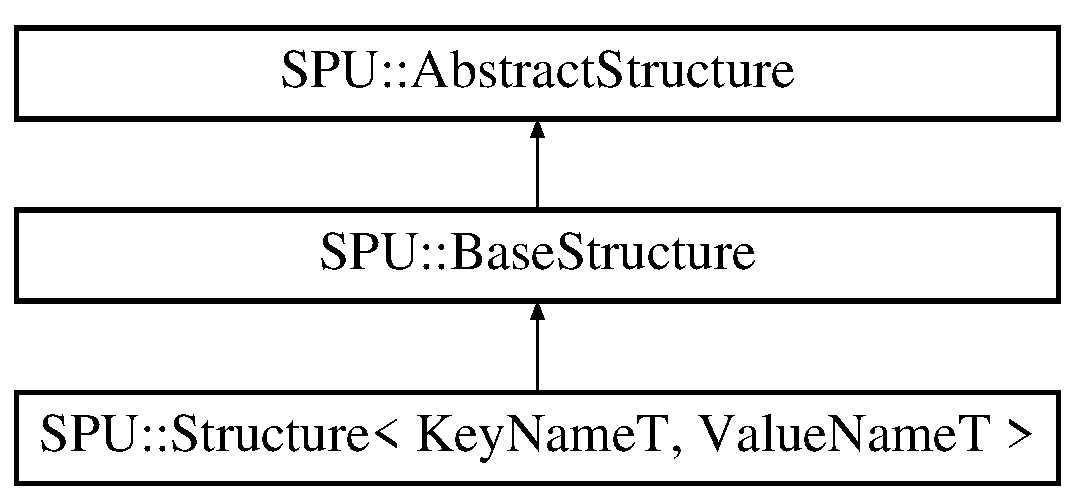
\includegraphics[height=3.000000cm]{class_s_p_u_1_1_structure}
\end{center}
\end{figure}
\subsection*{Открытые члены}
\begin{DoxyCompactItemize}
\item 
\mbox{\Hypertarget{class_s_p_u_1_1_structure_a1ba8a2044329b292bca47657c780814e}\label{class_s_p_u_1_1_structure_a1ba8a2044329b292bca47657c780814e}} 
{\bfseries Structure} (\hyperlink{class_s_p_u_1_1_fields_length}{Key\+Length} key\+\_\+length, bool is\+\_\+val\+\_\+constr=false)
\item 
\mbox{\Hypertarget{class_s_p_u_1_1_structure_a8f1fa54defe46c0e00e5a6238c787a67}\label{class_s_p_u_1_1_structure_a8f1fa54defe46c0e00e5a6238c787a67}} 
{\bfseries Structure} (\hyperlink{class_s_p_u_1_1_fields_length}{Value\+Length} value\+\_\+length)
\item 
\mbox{\Hypertarget{class_s_p_u_1_1_structure_a3de5498cf78a12a4035f95650bc79b81}\label{class_s_p_u_1_1_structure_a3de5498cf78a12a4035f95650bc79b81}} 
{\bfseries Structure} (\hyperlink{class_s_p_u_1_1_fields_length}{Key\+Length} key\+\_\+length, \hyperlink{class_s_p_u_1_1_fields_length}{Value\+Length} value\+\_\+length)
\item 
\mbox{\Hypertarget{class_s_p_u_1_1_structure_a1f8300c2f83593861eb28cca1f325566}\label{class_s_p_u_1_1_structure_a1f8300c2f83593861eb28cca1f325566}} 
\hyperlink{class_s_p_u_1_1_fields_pointer}{Key\+Pointer} {\bfseries key} ()
\item 
\mbox{\Hypertarget{class_s_p_u_1_1_structure_a01afbdf0a4361daeccf06d8e9f705b44}\label{class_s_p_u_1_1_structure_a01afbdf0a4361daeccf06d8e9f705b44}} 
\hyperlink{class_s_p_u_1_1_fields_pointer}{Value\+Pointer} {\bfseries value} ()
\item 
\mbox{\Hypertarget{class_s_p_u_1_1_structure_aacf3f53ac5881d1501fd463177e8d134}\label{class_s_p_u_1_1_structure_aacf3f53ac5881d1501fd463177e8d134}} 
status\+\_\+t {\bfseries insert} (key\+\_\+t key, value\+\_\+t value, flags\+\_\+t flags=N\+O\+\_\+\+F\+L\+A\+GS)
\item 
\mbox{\Hypertarget{class_s_p_u_1_1_structure_a014733e99be0d1f989c905355e4e17e0}\label{class_s_p_u_1_1_structure_a014733e99be0d1f989c905355e4e17e0}} 
status\+\_\+t {\bfseries insert} (\hyperlink{class_s_p_u_1_1_fields_data}{Key\+Data} key, value\+\_\+t value, flags\+\_\+t flags=N\+O\+\_\+\+F\+L\+A\+GS)
\item 
\mbox{\Hypertarget{class_s_p_u_1_1_structure_aa99577c268a263c434ba960dfea39b72}\label{class_s_p_u_1_1_structure_aa99577c268a263c434ba960dfea39b72}} 
status\+\_\+t {\bfseries insert} (key\+\_\+t key, \hyperlink{class_s_p_u_1_1_fields_data}{Value\+Data} value, flags\+\_\+t flags=N\+O\+\_\+\+F\+L\+A\+GS)
\item 
\mbox{\Hypertarget{class_s_p_u_1_1_structure_a9e104419b60f39753c5c28612b7114cf}\label{class_s_p_u_1_1_structure_a9e104419b60f39753c5c28612b7114cf}} 
status\+\_\+t {\bfseries insert} (\hyperlink{class_s_p_u_1_1_fields_data}{Key\+Data} key, \hyperlink{class_s_p_u_1_1_fields_data}{Value\+Data} value, flags\+\_\+t flags=N\+O\+\_\+\+F\+L\+A\+GS)
\item 
\mbox{\Hypertarget{class_s_p_u_1_1_structure_a6f02f8920af440d35dae6033ee43c1ff}\label{class_s_p_u_1_1_structure_a6f02f8920af440d35dae6033ee43c1ff}} 
status\+\_\+t {\bfseries del} (key\+\_\+t key, flags\+\_\+t flags=N\+O\+\_\+\+F\+L\+A\+GS)
\item 
\mbox{\Hypertarget{class_s_p_u_1_1_structure_a2b032f6a655aa3133bdcc2bc2bfb8353}\label{class_s_p_u_1_1_structure_a2b032f6a655aa3133bdcc2bc2bfb8353}} 
status\+\_\+t {\bfseries del} (\hyperlink{class_s_p_u_1_1_fields_data}{Key\+Data} key, flags\+\_\+t flags=N\+O\+\_\+\+F\+L\+A\+GS)
\item 
\mbox{\Hypertarget{class_s_p_u_1_1_structure_a97c83eb715f31cebd64b52601a80286a}\label{class_s_p_u_1_1_structure_a97c83eb715f31cebd64b52601a80286a}} 
\hyperlink{struct_s_p_u_1_1pair__containter}{pair\+\_\+t} {\bfseries search} (key\+\_\+t key, flags\+\_\+t flags=P\+\_\+\+F\+L\+AG)
\item 
\mbox{\Hypertarget{class_s_p_u_1_1_structure_a0693f4b7028f1ea3dc58ddf7a039e49b}\label{class_s_p_u_1_1_structure_a0693f4b7028f1ea3dc58ddf7a039e49b}} 
\hyperlink{struct_s_p_u_1_1pair__containter}{pair\+\_\+t} {\bfseries search} (\hyperlink{class_s_p_u_1_1_fields_data}{Key\+Data} key, flags\+\_\+t flags=P\+\_\+\+F\+L\+AG)
\item 
\mbox{\Hypertarget{class_s_p_u_1_1_structure_a7da5feeec46c1022b0372b5e0b7ed876}\label{class_s_p_u_1_1_structure_a7da5feeec46c1022b0372b5e0b7ed876}} 
\hyperlink{struct_s_p_u_1_1pair__containter}{pair\+\_\+t} {\bfseries min} (flags\+\_\+t flags=P\+\_\+\+F\+L\+AG)
\item 
\mbox{\Hypertarget{class_s_p_u_1_1_structure_ae0a0e396a6a0ea5017372a76bf223d4c}\label{class_s_p_u_1_1_structure_ae0a0e396a6a0ea5017372a76bf223d4c}} 
\hyperlink{struct_s_p_u_1_1pair__containter}{pair\+\_\+t} {\bfseries max} (flags\+\_\+t flags=P\+\_\+\+F\+L\+AG)
\item 
\mbox{\Hypertarget{class_s_p_u_1_1_structure_ad4f8e7b76d663328555564609135aa2e}\label{class_s_p_u_1_1_structure_ad4f8e7b76d663328555564609135aa2e}} 
\hyperlink{struct_s_p_u_1_1pair__containter}{pair\+\_\+t} {\bfseries next} (key\+\_\+t key, flags\+\_\+t flags=P\+\_\+\+F\+L\+AG)
\item 
\mbox{\Hypertarget{class_s_p_u_1_1_structure_a0c941cc613d2384c55a6be5a411516ba}\label{class_s_p_u_1_1_structure_a0c941cc613d2384c55a6be5a411516ba}} 
\hyperlink{struct_s_p_u_1_1pair__containter}{pair\+\_\+t} {\bfseries next} (\hyperlink{class_s_p_u_1_1_fields_data}{Key\+Data} key, flags\+\_\+t flags=P\+\_\+\+F\+L\+AG)
\item 
\mbox{\Hypertarget{class_s_p_u_1_1_structure_aac3de28a91bdd655b8bccc550b8556f7}\label{class_s_p_u_1_1_structure_aac3de28a91bdd655b8bccc550b8556f7}} 
\hyperlink{struct_s_p_u_1_1pair__containter}{pair\+\_\+t} {\bfseries prev} (key\+\_\+t key, flags\+\_\+t flags=P\+\_\+\+F\+L\+AG)
\item 
\mbox{\Hypertarget{class_s_p_u_1_1_structure_a2a5c83c2fd203ef6a9fefd990614edfc}\label{class_s_p_u_1_1_structure_a2a5c83c2fd203ef6a9fefd990614edfc}} 
\hyperlink{struct_s_p_u_1_1pair__containter}{pair\+\_\+t} {\bfseries prev} (\hyperlink{class_s_p_u_1_1_fields_data}{Key\+Data} key, flags\+\_\+t flags=P\+\_\+\+F\+L\+AG)
\item 
\mbox{\Hypertarget{class_s_p_u_1_1_structure_a9d7b107363dccd412d386807e6354c15}\label{class_s_p_u_1_1_structure_a9d7b107363dccd412d386807e6354c15}} 
\hyperlink{struct_s_p_u_1_1pair__containter}{pair\+\_\+t} {\bfseries nsm} (key\+\_\+t key, flags\+\_\+t flags=P\+\_\+\+F\+L\+AG)
\item 
\mbox{\Hypertarget{class_s_p_u_1_1_structure_a2a056bd23cc2951c101d19f2a76d77f6}\label{class_s_p_u_1_1_structure_a2a056bd23cc2951c101d19f2a76d77f6}} 
\hyperlink{struct_s_p_u_1_1pair__containter}{pair\+\_\+t} {\bfseries nsm} (\hyperlink{class_s_p_u_1_1_fields_data}{Key\+Data} key, flags\+\_\+t flags=P\+\_\+\+F\+L\+AG)
\item 
\mbox{\Hypertarget{class_s_p_u_1_1_structure_a44f845d26a28b753119cd07fdf50c52d}\label{class_s_p_u_1_1_structure_a44f845d26a28b753119cd07fdf50c52d}} 
\hyperlink{struct_s_p_u_1_1pair__containter}{pair\+\_\+t} {\bfseries ngr} (key\+\_\+t key, flags\+\_\+t flags=P\+\_\+\+F\+L\+AG)
\item 
\mbox{\Hypertarget{class_s_p_u_1_1_structure_aa66ccc48dc6fff3d3518ce60a3a0c431}\label{class_s_p_u_1_1_structure_aa66ccc48dc6fff3d3518ce60a3a0c431}} 
\hyperlink{struct_s_p_u_1_1pair__containter}{pair\+\_\+t} {\bfseries ngr} (\hyperlink{class_s_p_u_1_1_fields_data}{Key\+Data} key, flags\+\_\+t flags=P\+\_\+\+F\+L\+AG)
\end{DoxyCompactItemize}
\subsection*{Защищенные члены}
\begin{DoxyCompactItemize}
\item 
\mbox{\Hypertarget{class_s_p_u_1_1_structure_ade8084a87ca74a587af1d8650347c682}\label{class_s_p_u_1_1_structure_ade8084a87ca74a587af1d8650347c682}} 
\hyperlink{struct_s_p_u_1_1pair__containter}{pair\+\_\+t} {\bfseries set\+\_\+pair} (\hyperlink{struct_s_p_u_1_1pair__containter}{pair\+\_\+t} pair)
\end{DoxyCompactItemize}
\subsection*{Дополнительные унаследованные члены}


Объявления и описания членов класса находятся в файле\+:\begin{DoxyCompactItemize}
\item 
spu-\/api/libspu/structure.\+hpp\end{DoxyCompactItemize}

\hypertarget{class_s_p_u_1_1_structure_3_01void_00_01void_01_4}{}\section{Шаблон класса S\+PU\+:\+:Structure$<$ void, void $>$}
\label{class_s_p_u_1_1_structure_3_01void_00_01void_01_4}\index{S\+P\+U\+::\+Structure$<$ void, void $>$@{S\+P\+U\+::\+Structure$<$ void, void $>$}}
Граф наследования\+:S\+PU\+:\+:Structure$<$ void, void $>$\+:\begin{figure}[H]
\begin{center}
\leavevmode
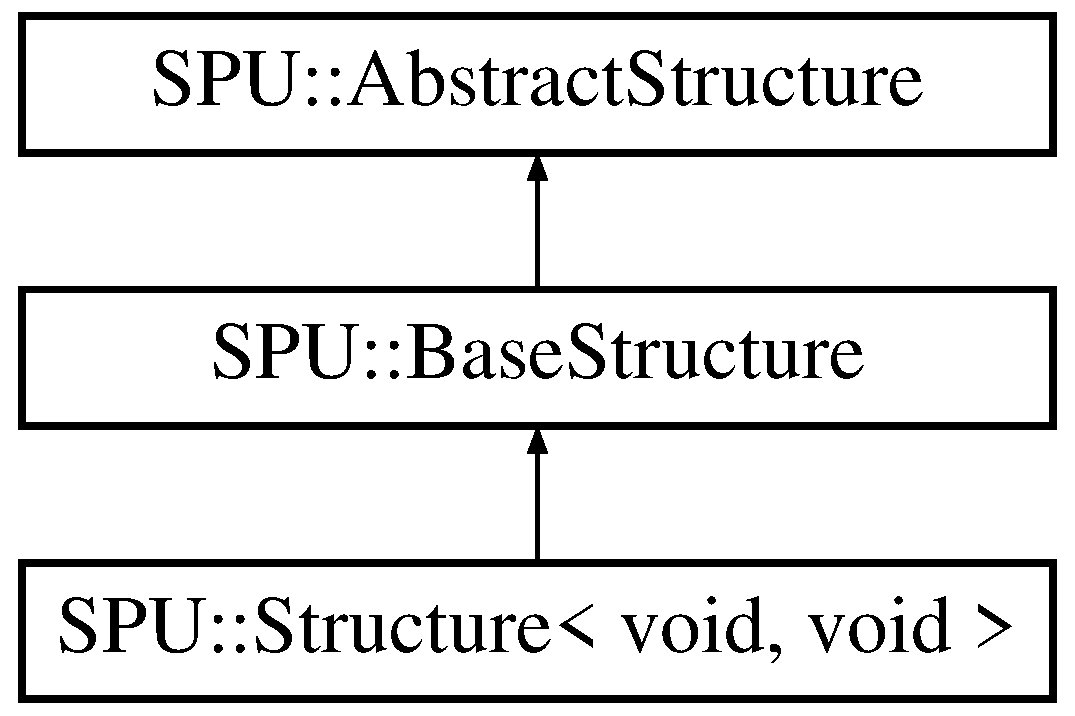
\includegraphics[height=3.000000cm]{class_s_p_u_1_1_structure_3_01void_00_01void_01_4}
\end{center}
\end{figure}
\subsection*{Дополнительные унаследованные члены}


Объявления и описания членов класса находятся в файле\+:\begin{DoxyCompactItemize}
\item 
spu-\/api/libspu/structure.\+hpp\end{DoxyCompactItemize}

\hypertarget{class_s_p_u___g_r_a_p_h_1_1_structure_iterator}{}\doxysection{Класс S\+P\+U\+\_\+\+G\+R\+A\+PH\+::Structure\+Iterator}
\label{class_s_p_u___g_r_a_p_h_1_1_structure_iterator}\index{SPU\_GRAPH::StructureIterator@{SPU\_GRAPH::StructureIterator}}
Граф наследования\+:S\+P\+U\+\_\+\+G\+R\+A\+PH\+::Structure\+Iterator\+:\begin{figure}[H]
\begin{center}
\leavevmode
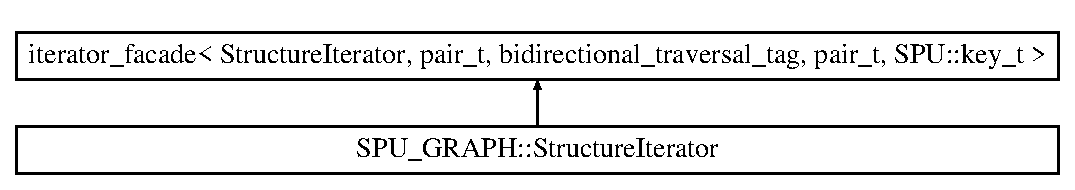
\includegraphics[height=2.000000cm]{class_s_p_u___g_r_a_p_h_1_1_structure_iterator}
\end{center}
\end{figure}
\doxysubsection*{Открытые члены}
\begin{DoxyCompactItemize}
\item 
\mbox{\Hypertarget{class_s_p_u___g_r_a_p_h_1_1_structure_iterator_a673249f944f5f9a2eb48e2de9cbda41e}\label{class_s_p_u___g_r_a_p_h_1_1_structure_iterator_a673249f944f5f9a2eb48e2de9cbda41e}} 
{\bfseries Structure\+Iterator} (const \mbox{\hyperlink{class_s_p_u___g_r_a_p_h_1_1_graph_structure}{Graph\+Structure}} $\ast$structure, S\+P\+U\+::key\+\_\+t key, S\+P\+U\+::key\+\_\+t end=0, S\+P\+U\+::status\+\_\+t status=I\+N\+I\+T\+\_\+\+S\+T\+A\+T\+US)
\item 
\mbox{\Hypertarget{class_s_p_u___g_r_a_p_h_1_1_structure_iterator_a94c72b8aa9b86fdc9a6e2e5269c0be8f}\label{class_s_p_u___g_r_a_p_h_1_1_structure_iterator_a94c72b8aa9b86fdc9a6e2e5269c0be8f}} 
\mbox{\hyperlink{struct_s_p_u_1_1pair__containter}{S\+P\+U\+::pair\+\_\+t}} {\bfseries dereference} () const
\item 
\mbox{\Hypertarget{class_s_p_u___g_r_a_p_h_1_1_structure_iterator_aec592dd9ddecca8f1fbd6bb7f3e523be}\label{class_s_p_u___g_r_a_p_h_1_1_structure_iterator_aec592dd9ddecca8f1fbd6bb7f3e523be}} 
bool {\bfseries equal} (const \mbox{\hyperlink{class_s_p_u___g_r_a_p_h_1_1_structure_iterator}{Structure\+Iterator}} \&other) const
\item 
\mbox{\Hypertarget{class_s_p_u___g_r_a_p_h_1_1_structure_iterator_ae4947b8b245fbb27fa3a5398fe02de28}\label{class_s_p_u___g_r_a_p_h_1_1_structure_iterator_ae4947b8b245fbb27fa3a5398fe02de28}} 
void {\bfseries increment} ()
\item 
\mbox{\Hypertarget{class_s_p_u___g_r_a_p_h_1_1_structure_iterator_a5ec155383d89c1e8b2a03d9b43a47414}\label{class_s_p_u___g_r_a_p_h_1_1_structure_iterator_a5ec155383d89c1e8b2a03d9b43a47414}} 
void {\bfseries decrement} ()
\end{DoxyCompactItemize}
\doxysubsection*{Друзья}
\begin{DoxyCompactItemize}
\item 
\mbox{\Hypertarget{class_s_p_u___g_r_a_p_h_1_1_structure_iterator_a0975271623c74c5b89bdf8d7fbce69c4}\label{class_s_p_u___g_r_a_p_h_1_1_structure_iterator_a0975271623c74c5b89bdf8d7fbce69c4}} 
class {\bfseries iterator\+\_\+core\+\_\+access}
\end{DoxyCompactItemize}


Объявления и описания членов класса находятся в файле\+:\begin{DoxyCompactItemize}
\item 
Structure\+Iterator.\+h\end{DoxyCompactItemize}

\hypertarget{class_s_p_u___g_r_a_p_h_1_1_structure_range}{}\doxysection{Класс S\+P\+U\+\_\+\+G\+R\+A\+PH\+::Structure\+Range}
\label{class_s_p_u___g_r_a_p_h_1_1_structure_range}\index{SPU\_GRAPH::StructureRange@{SPU\_GRAPH::StructureRange}}


Контейнер, кот. содержит ключи в диапозоне \mbox{[}start..end\mbox{]}, start и end входят в диаопозон.  




{\ttfamily \#include $<$Structure\+Iterator.\+h$>$}

\doxysubsection*{Открытые типы}
\begin{DoxyCompactItemize}
\item 
\mbox{\Hypertarget{class_s_p_u___g_r_a_p_h_1_1_structure_range_a952af08b4955e6cd840cb86cfa707685}\label{class_s_p_u___g_r_a_p_h_1_1_structure_range_a952af08b4955e6cd840cb86cfa707685}} 
typedef \mbox{\hyperlink{class_s_p_u___g_r_a_p_h_1_1_structure_iterator}{Structure\+Iterator}} {\bfseries iterator}
\end{DoxyCompactItemize}
\doxysubsection*{Открытые члены}
\begin{DoxyCompactItemize}
\item 
\mbox{\Hypertarget{class_s_p_u___g_r_a_p_h_1_1_structure_range_a0e7272cf854f063e26354cbdca78ae82}\label{class_s_p_u___g_r_a_p_h_1_1_structure_range_a0e7272cf854f063e26354cbdca78ae82}} 
{\bfseries Structure\+Range} (const \mbox{\hyperlink{class_s_p_u___g_r_a_p_h_1_1_graph_structure}{Graph\+Structure}} $\ast$structure, S\+P\+U\+::key\+\_\+t start, S\+P\+U\+::key\+\_\+t end)
\item 
\mbox{\Hypertarget{class_s_p_u___g_r_a_p_h_1_1_structure_range_ae01654e46347e70c9e71743db1c170c0}\label{class_s_p_u___g_r_a_p_h_1_1_structure_range_ae01654e46347e70c9e71743db1c170c0}} 
\mbox{\hyperlink{class_s_p_u___g_r_a_p_h_1_1_structure_iterator}{iterator}} {\bfseries begin} ()
\item 
\mbox{\Hypertarget{class_s_p_u___g_r_a_p_h_1_1_structure_range_a5f3b36929787a423acd58f4836d54b38}\label{class_s_p_u___g_r_a_p_h_1_1_structure_range_a5f3b36929787a423acd58f4836d54b38}} 
\mbox{\hyperlink{class_s_p_u___g_r_a_p_h_1_1_structure_iterator}{iterator}} {\bfseries end} ()
\end{DoxyCompactItemize}


\doxysubsection{Подробное описание}
Контейнер, кот. содержит ключи в диапозоне \mbox{[}start..end\mbox{]}, start и end входят в диаопозон. 

Объявления и описания членов класса находятся в файле\+:\begin{DoxyCompactItemize}
\item 
Structure\+Iterator.\+h\end{DoxyCompactItemize}

\hypertarget{classvertex__property__writer}{}\doxysection{Класс vertex\+\_\+property\+\_\+writer}
\label{classvertex__property__writer}\index{vertex\_property\_writer@{vertex\_property\_writer}}
\doxysubsection*{Открытые члены}
\begin{DoxyCompactItemize}
\item 
\mbox{\Hypertarget{classvertex__property__writer_ab69d3dcb19e388676458dc1e972b8a44}\label{classvertex__property__writer_ab69d3dcb19e388676458dc1e972b8a44}} 
{\bfseries vertex\+\_\+property\+\_\+writer} (\mbox{\hyperlink{class_s_p_u___g_r_a_p_h_1_1_spu_ultra_graph}{Spu\+Ultra\+Graph}} \&g)
\item 
\mbox{\Hypertarget{classvertex__property__writer_a42b7a6dc52b543dd3ac07f031b0cf793}\label{classvertex__property__writer_a42b7a6dc52b543dd3ac07f031b0cf793}} 
void {\bfseries operator()} (std\+::ostream \&out, const Spu\+Ultra\+Graph\+::vertex\+\_\+descriptor \&v) const
\item 
\mbox{\Hypertarget{classvertex__property__writer_ab69d3dcb19e388676458dc1e972b8a44}\label{classvertex__property__writer_ab69d3dcb19e388676458dc1e972b8a44}} 
{\bfseries vertex\+\_\+property\+\_\+writer} (\mbox{\hyperlink{class_s_p_u___g_r_a_p_h_1_1_spu_ultra_graph}{Spu\+Ultra\+Graph}} \&g)
\item 
\mbox{\Hypertarget{classvertex__property__writer_a42b7a6dc52b543dd3ac07f031b0cf793}\label{classvertex__property__writer_a42b7a6dc52b543dd3ac07f031b0cf793}} 
void {\bfseries operator()} (std\+::ostream \&out, const Spu\+Ultra\+Graph\+::vertex\+\_\+descriptor \&v) const
\end{DoxyCompactItemize}


Объявления и описания членов классов находятся в файлах\+:\begin{DoxyCompactItemize}
\item 
examples/dijkstra\+\_\+example.\+cpp\item 
examples/graphvis\+\_\+example.\+cpp\end{DoxyCompactItemize}

\hypertarget{class_s_p_u___g_r_a_p_h_1_1_spu_ultra_graph_1_1_vertex_iterator}{}\section{Класс S\+P\+U\+\_\+\+G\+R\+A\+PH\+:\+:Spu\+Ultra\+Graph\+:\+:Vertex\+Iterator}
\label{class_s_p_u___g_r_a_p_h_1_1_spu_ultra_graph_1_1_vertex_iterator}\index{S\+P\+U\+\_\+\+G\+R\+A\+P\+H\+::\+Spu\+Ultra\+Graph\+::\+Vertex\+Iterator@{S\+P\+U\+\_\+\+G\+R\+A\+P\+H\+::\+Spu\+Ultra\+Graph\+::\+Vertex\+Iterator}}
Граф наследования\+:S\+P\+U\+\_\+\+G\+R\+A\+PH\+:\+:Spu\+Ultra\+Graph\+:\+:Vertex\+Iterator\+:\begin{figure}[H]
\begin{center}
\leavevmode
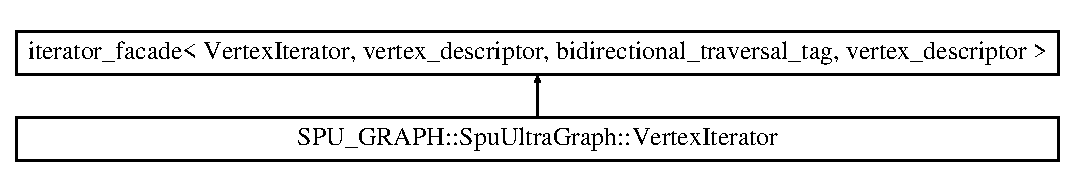
\includegraphics[height=1.924399cm]{class_s_p_u___g_r_a_p_h_1_1_spu_ultra_graph_1_1_vertex_iterator}
\end{center}
\end{figure}
\subsection*{Открытые члены}
\begin{DoxyCompactItemize}
\item 
\mbox{\Hypertarget{class_s_p_u___g_r_a_p_h_1_1_spu_ultra_graph_1_1_vertex_iterator_a44ad1919b43f91727e32b97bc4a26801}\label{class_s_p_u___g_r_a_p_h_1_1_spu_ultra_graph_1_1_vertex_iterator_a44ad1919b43f91727e32b97bc4a26801}} 
{\bfseries Vertex\+Iterator} (const \hyperlink{class_s_p_u___g_r_a_p_h_1_1_spu_ultra_graph}{Spu\+Ultra\+Graph} $\ast$g, vertex\+\_\+descriptor v=0)
\item 
\mbox{\Hypertarget{class_s_p_u___g_r_a_p_h_1_1_spu_ultra_graph_1_1_vertex_iterator_ad631b16614705649ab2fb57dd9173664}\label{class_s_p_u___g_r_a_p_h_1_1_spu_ultra_graph_1_1_vertex_iterator_ad631b16614705649ab2fb57dd9173664}} 
vertex\+\_\+descriptor {\bfseries dereference} () const
\item 
\mbox{\Hypertarget{class_s_p_u___g_r_a_p_h_1_1_spu_ultra_graph_1_1_vertex_iterator_a6bbd7e9d20bcb9e265ebfb3aeb88535e}\label{class_s_p_u___g_r_a_p_h_1_1_spu_ultra_graph_1_1_vertex_iterator_a6bbd7e9d20bcb9e265ebfb3aeb88535e}} 
bool {\bfseries equal} (const \hyperlink{class_s_p_u___g_r_a_p_h_1_1_spu_ultra_graph_1_1_vertex_iterator}{Vertex\+Iterator} \&other) const
\item 
\mbox{\Hypertarget{class_s_p_u___g_r_a_p_h_1_1_spu_ultra_graph_1_1_vertex_iterator_ae2da860f819452beb1db75862bda88ef}\label{class_s_p_u___g_r_a_p_h_1_1_spu_ultra_graph_1_1_vertex_iterator_ae2da860f819452beb1db75862bda88ef}} 
void {\bfseries increment} ()
\item 
\mbox{\Hypertarget{class_s_p_u___g_r_a_p_h_1_1_spu_ultra_graph_1_1_vertex_iterator_a99a6b17f75f1847ba21dc3a400bfc36b}\label{class_s_p_u___g_r_a_p_h_1_1_spu_ultra_graph_1_1_vertex_iterator_a99a6b17f75f1847ba21dc3a400bfc36b}} 
void {\bfseries decrement} ()
\end{DoxyCompactItemize}
\subsection*{Друзья}
\begin{DoxyCompactItemize}
\item 
\mbox{\Hypertarget{class_s_p_u___g_r_a_p_h_1_1_spu_ultra_graph_1_1_vertex_iterator_a0975271623c74c5b89bdf8d7fbce69c4}\label{class_s_p_u___g_r_a_p_h_1_1_spu_ultra_graph_1_1_vertex_iterator_a0975271623c74c5b89bdf8d7fbce69c4}} 
class {\bfseries iterator\+\_\+core\+\_\+access}
\end{DoxyCompactItemize}


Объявления и описания членов классов находятся в файлах\+:\begin{DoxyCompactItemize}
\item 
Spu\+Ultra\+Graph.\+h\item 
Spu\+Ultra\+Graph.\+cpp\end{DoxyCompactItemize}

\hypertarget{class_s_p_u___g_r_a_p_h_1_1_spu_ultra_graph_1_1_vertices}{}\section{Класс S\+P\+U\+\_\+\+G\+R\+A\+PH\+:\+:Spu\+Ultra\+Graph\+:\+:Vertices}
\label{class_s_p_u___g_r_a_p_h_1_1_spu_ultra_graph_1_1_vertices}\index{S\+P\+U\+\_\+\+G\+R\+A\+P\+H\+::\+Spu\+Ultra\+Graph\+::\+Vertices@{S\+P\+U\+\_\+\+G\+R\+A\+P\+H\+::\+Spu\+Ultra\+Graph\+::\+Vertices}}


Контейнер содержащий все ребра графа  




{\ttfamily \#include $<$Spu\+Ultra\+Graph.\+h$>$}

\subsection*{Открытые типы}
\begin{DoxyCompactItemize}
\item 
\mbox{\Hypertarget{class_s_p_u___g_r_a_p_h_1_1_spu_ultra_graph_1_1_vertices_a749538579b8dbb828f054e0d21566e19}\label{class_s_p_u___g_r_a_p_h_1_1_spu_ultra_graph_1_1_vertices_a749538579b8dbb828f054e0d21566e19}} 
typedef \hyperlink{class_s_p_u___g_r_a_p_h_1_1_spu_ultra_graph_a06163cbc87b2e49334b4bcc46c7b0c89}{vertex\+\_\+iterator} {\bfseries iterator}
\end{DoxyCompactItemize}
\subsection*{Открытые члены}
\begin{DoxyCompactItemize}
\item 
\mbox{\Hypertarget{class_s_p_u___g_r_a_p_h_1_1_spu_ultra_graph_1_1_vertices_a6419ca4f357385cd5693df5ed1c59aa2}\label{class_s_p_u___g_r_a_p_h_1_1_spu_ultra_graph_1_1_vertices_a6419ca4f357385cd5693df5ed1c59aa2}} 
{\bfseries Vertices} (const \hyperlink{class_s_p_u___g_r_a_p_h_1_1_spu_ultra_graph}{Spu\+Ultra\+Graph} $\ast$g)
\item 
\mbox{\Hypertarget{class_s_p_u___g_r_a_p_h_1_1_spu_ultra_graph_1_1_vertices_a845ca204fed6736b8aae37ad434305f0}\label{class_s_p_u___g_r_a_p_h_1_1_spu_ultra_graph_1_1_vertices_a845ca204fed6736b8aae37ad434305f0}} 
\hyperlink{class_s_p_u___g_r_a_p_h_1_1_spu_ultra_graph_1_1_vertex_iterator}{iterator} {\bfseries begin} ()
\item 
\mbox{\Hypertarget{class_s_p_u___g_r_a_p_h_1_1_spu_ultra_graph_1_1_vertices_adb424c5238d309370ccb0a6a6dbf7b07}\label{class_s_p_u___g_r_a_p_h_1_1_spu_ultra_graph_1_1_vertices_adb424c5238d309370ccb0a6a6dbf7b07}} 
\hyperlink{class_s_p_u___g_r_a_p_h_1_1_spu_ultra_graph_1_1_vertex_iterator}{iterator} {\bfseries end} ()
\end{DoxyCompactItemize}


\subsection{Подробное описание}
Контейнер содержащий все ребра графа 

Объявления и описания членов класса находятся в файле\+:\begin{DoxyCompactItemize}
\item 
Spu\+Ultra\+Graph.\+h\end{DoxyCompactItemize}

%--- End generated contents ---

% Index
\backmatter
\newpage
\phantomsection
\clearemptydoublepage
\addcontentsline{toc}{chapter}{Алфавитный указатель}
\printindex

\end{document}
